% Options for packages loaded elsewhere
\PassOptionsToPackage{unicode}{hyperref}
\PassOptionsToPackage{hyphens}{url}
%
\documentclass[
]{book}
\usepackage{amsmath,amssymb}
\usepackage{iftex}
\ifPDFTeX
  \usepackage[T1]{fontenc}
  \usepackage[utf8]{inputenc}
  \usepackage{textcomp} % provide euro and other symbols
\else % if luatex or xetex
  \usepackage{unicode-math} % this also loads fontspec
  \defaultfontfeatures{Scale=MatchLowercase}
  \defaultfontfeatures[\rmfamily]{Ligatures=TeX,Scale=1}
\fi
\usepackage{lmodern}
\ifPDFTeX\else
  % xetex/luatex font selection
    \setmainfont[]{Arial}
\fi
% Use upquote if available, for straight quotes in verbatim environments
\IfFileExists{upquote.sty}{\usepackage{upquote}}{}
\IfFileExists{microtype.sty}{% use microtype if available
  \usepackage[]{microtype}
  \UseMicrotypeSet[protrusion]{basicmath} % disable protrusion for tt fonts
}{}
\makeatletter
\@ifundefined{KOMAClassName}{% if non-KOMA class
  \IfFileExists{parskip.sty}{%
    \usepackage{parskip}
  }{% else
    \setlength{\parindent}{0pt}
    \setlength{\parskip}{6pt plus 2pt minus 1pt}}
}{% if KOMA class
  \KOMAoptions{parskip=half}}
\makeatother
\usepackage{xcolor}
\usepackage{color}
\usepackage{fancyvrb}
\newcommand{\VerbBar}{|}
\newcommand{\VERB}{\Verb[commandchars=\\\{\}]}
\DefineVerbatimEnvironment{Highlighting}{Verbatim}{commandchars=\\\{\}}
% Add ',fontsize=\small' for more characters per line
\usepackage{framed}
\definecolor{shadecolor}{RGB}{248,248,248}
\newenvironment{Shaded}{\begin{snugshade}}{\end{snugshade}}
\newcommand{\AlertTok}[1]{\textcolor[rgb]{0.94,0.16,0.16}{#1}}
\newcommand{\AnnotationTok}[1]{\textcolor[rgb]{0.56,0.35,0.01}{\textbf{\textit{#1}}}}
\newcommand{\AttributeTok}[1]{\textcolor[rgb]{0.13,0.29,0.53}{#1}}
\newcommand{\BaseNTok}[1]{\textcolor[rgb]{0.00,0.00,0.81}{#1}}
\newcommand{\BuiltInTok}[1]{#1}
\newcommand{\CharTok}[1]{\textcolor[rgb]{0.31,0.60,0.02}{#1}}
\newcommand{\CommentTok}[1]{\textcolor[rgb]{0.56,0.35,0.01}{\textit{#1}}}
\newcommand{\CommentVarTok}[1]{\textcolor[rgb]{0.56,0.35,0.01}{\textbf{\textit{#1}}}}
\newcommand{\ConstantTok}[1]{\textcolor[rgb]{0.56,0.35,0.01}{#1}}
\newcommand{\ControlFlowTok}[1]{\textcolor[rgb]{0.13,0.29,0.53}{\textbf{#1}}}
\newcommand{\DataTypeTok}[1]{\textcolor[rgb]{0.13,0.29,0.53}{#1}}
\newcommand{\DecValTok}[1]{\textcolor[rgb]{0.00,0.00,0.81}{#1}}
\newcommand{\DocumentationTok}[1]{\textcolor[rgb]{0.56,0.35,0.01}{\textbf{\textit{#1}}}}
\newcommand{\ErrorTok}[1]{\textcolor[rgb]{0.64,0.00,0.00}{\textbf{#1}}}
\newcommand{\ExtensionTok}[1]{#1}
\newcommand{\FloatTok}[1]{\textcolor[rgb]{0.00,0.00,0.81}{#1}}
\newcommand{\FunctionTok}[1]{\textcolor[rgb]{0.13,0.29,0.53}{\textbf{#1}}}
\newcommand{\ImportTok}[1]{#1}
\newcommand{\InformationTok}[1]{\textcolor[rgb]{0.56,0.35,0.01}{\textbf{\textit{#1}}}}
\newcommand{\KeywordTok}[1]{\textcolor[rgb]{0.13,0.29,0.53}{\textbf{#1}}}
\newcommand{\NormalTok}[1]{#1}
\newcommand{\OperatorTok}[1]{\textcolor[rgb]{0.81,0.36,0.00}{\textbf{#1}}}
\newcommand{\OtherTok}[1]{\textcolor[rgb]{0.56,0.35,0.01}{#1}}
\newcommand{\PreprocessorTok}[1]{\textcolor[rgb]{0.56,0.35,0.01}{\textit{#1}}}
\newcommand{\RegionMarkerTok}[1]{#1}
\newcommand{\SpecialCharTok}[1]{\textcolor[rgb]{0.81,0.36,0.00}{\textbf{#1}}}
\newcommand{\SpecialStringTok}[1]{\textcolor[rgb]{0.31,0.60,0.02}{#1}}
\newcommand{\StringTok}[1]{\textcolor[rgb]{0.31,0.60,0.02}{#1}}
\newcommand{\VariableTok}[1]{\textcolor[rgb]{0.00,0.00,0.00}{#1}}
\newcommand{\VerbatimStringTok}[1]{\textcolor[rgb]{0.31,0.60,0.02}{#1}}
\newcommand{\WarningTok}[1]{\textcolor[rgb]{0.56,0.35,0.01}{\textbf{\textit{#1}}}}
\usepackage{longtable,booktabs,array}
\usepackage{calc} % for calculating minipage widths
% Correct order of tables after \paragraph or \subparagraph
\usepackage{etoolbox}
\makeatletter
\patchcmd\longtable{\par}{\if@noskipsec\mbox{}\fi\par}{}{}
\makeatother
% Allow footnotes in longtable head/foot
\IfFileExists{footnotehyper.sty}{\usepackage{footnotehyper}}{\usepackage{footnote}}
\makesavenoteenv{longtable}
\usepackage{graphicx}
\makeatletter
\def\maxwidth{\ifdim\Gin@nat@width>\linewidth\linewidth\else\Gin@nat@width\fi}
\def\maxheight{\ifdim\Gin@nat@height>\textheight\textheight\else\Gin@nat@height\fi}
\makeatother
% Scale images if necessary, so that they will not overflow the page
% margins by default, and it is still possible to overwrite the defaults
% using explicit options in \includegraphics[width, height, ...]{}
\setkeys{Gin}{width=\maxwidth,height=\maxheight,keepaspectratio}
% Set default figure placement to htbp
\makeatletter
\def\fps@figure{htbp}
\makeatother
\setlength{\emergencystretch}{3em} % prevent overfull lines
\providecommand{\tightlist}{%
  \setlength{\itemsep}{0pt}\setlength{\parskip}{0pt}}
\setcounter{secnumdepth}{5}
\usepackage{booktabs}
\usepackage{amsthm}
\makeatletter
\def\thm@space@setup{%
  \thm@preskip=8pt plus 2pt minus 4pt
  \thm@postskip=\thm@preskip
}
\makeatother
\ifLuaTeX
  \usepackage{selnolig}  % disable illegal ligatures
\fi
\usepackage[]{natbib}
\bibliographystyle{apalike}
\usepackage{bookmark}
\IfFileExists{xurl.sty}{\usepackage{xurl}}{} % add URL line breaks if available
\urlstyle{same}
\hypersetup{
  pdftitle={Разработка telegram ботов на языке R},
  pdfauthor={Алексей Селезнёв},
  hidelinks,
  pdfcreator={LaTeX via pandoc}}

\title{Разработка telegram ботов на языке R}
\author{Алексей Селезнёв}
\date{2025-04-27}

\begin{document}
\maketitle

{
\setcounter{tocdepth}{1}
\tableofcontents
}
\chapter*{Введение}\label{ux432ux432ux435ux434ux435ux43dux438ux435}
\addcontentsline{toc}{chapter}{Введение}

\begin{center}\rule{0.5\linewidth}{0.5pt}\end{center}

Аудитория Telegram растёт с геометрической прогрессией. Популярность мессенджера объясняется его удобством, наличием каналов и чатов, а также возможностью создавать ботов.

Боты могут использоваться для самых разных задач: от автоматизации общения с клиентами до управления личными делами и автоматизации рутинных задач. С их помощью можно выполнять практически любые операции: отправлять и запрашивать данные, запускать задачи на сервере, собирать информацию в базу данных, отправлять электронные письма и многое другое. Т.е. telegram бот может стать интерфейсом для выполнения любых ваших задач.

Этот веб-учебник научит вас разрабатывать Telegram-ботов на языке программирования R. Материал изложен последовательно: от простого к сложному.

В первой главе мы рассмотрим, как отправлять сообщения из R в Telegram, к четвёртой главе мы создадим полноценного бота, который сможет вести логический диалог с пользователем, а далее расмотрим ещё несколько смежных тем, разберёмся с контейнерезацией приложений, и запуском ботов в облачных платформах.

Основным R-пакетом, который мы будем использовать на протяжении всего учебника, является telegram.bot. Каждая глава завершается небольшим заданием и тестом, чтобы вы могли проверить свои знания и понять, насколько хорошо усвоили материал.

\section*{Навыки необходимые для прохождения учебника}\label{ux43dux430ux432ux44bux43aux438-ux43dux435ux43eux431ux445ux43eux434ux438ux43cux44bux435-ux434ux43bux44f-ux43fux440ux43eux445ux43eux436ux434ux435ux43dux438ux44f-ux443ux447ux435ux431ux43dux438ux43aux430}
\addcontentsline{toc}{section}{Навыки необходимые для прохождения учебника}

Тему построения ботов я отношу к продвинутым навыкам, не зависимо от выбранного язка программирования. Поэтому в этой книге не рассматриваются базовые вводные темы по основам языка R.

Для чтения и понимания книги вам необходимо обладать следующими навыками на языке программирования R:

\begin{itemize}
\tightlist
\item
  Понимать базовые програмные конструкции, т.е. циклы и условные ветвления.
\item
  Понимать что такое функция.
\item
  Разбираться в основных структурах данных языка.
\item
  Уметь работать со строками.
\item
  Владеть основами манипуляции данных с помощью пакета \texttt{dplyr}.
\item
  Иметь поверхностное понимание о том, что такое API.
\end{itemize}

Перечисленные выше темы выходят за рамки этой книги, но подробно рассматриваются в онлайн академии \href{https://r-for-marketing.netpeak.net/}{``Язык R для интернет-маркетинга''}.

\section*{Об авторе}\label{ux43eux431-ux430ux432ux442ux43eux440ux435}
\addcontentsline{toc}{section}{Об авторе}

Меня зовут Алексей Селезнёв, и я уже более 10 лет работаю аналитиком. С 2016 года руковожу отделом аналитики в агентстве интернет-маркетинга Netpeak.

Являюсь автором курсов по языку R:

\begin{itemize}
\tightlist
\item
  \href{https://selesnow.github.io/r4excel_users/}{Язык R для пользователей Excel}.
\item
  \href{https://selesnow.github.io/dplyr_1_0_0_course/}{Введение в dplyr 1.0.0}.
\item
  \href{https://selesnow.github.io/iterations_in_r/}{Циклы и функционалы в языке R}.
\item
  \href{https://selesnow.github.io/r_package_course/}{Разработка пакетов на языке R}.
\item
  \href{https://www.youtube.com/playlist?list=PLD2LDq8edf4o6dSZ4BIr7J08gT97nimH_}{Язык R для интернет-маркетинга}.
\end{itemize}

Неоднократно выступал в роли спикера на различных конференция посвящённых аналитике и маркетингу, среди которых: 8P, Матемаркениг, Analyze, Ecommerce, GoAnalytics и другие.

Являюсь автором ряда R пакетов опубликованных в CRAN: rgoogleads, rfacebookstat, timesperiodR и др.

С 2015 года активно публикую статьи по аналитике; на момент написания этих строк у меня более 120 публикаций в различных интернет-изданиях. Веду собственный \href{https://alexeyseleznev.wordpress.com/}{блог}, который служит агрегатором моих статей с различных источников.

В 2018 году я создал Telegram-канал \href{https://t.me/R4marketing}{R4marketing}, где делюсь полезными русскоязычными материалами по языку R: ссылками на статьи, доклады, вебинары и заметками. В 2020 году запустил \href{https://bit.ly/36kliAp}{YouTube канал} с видеоуроками по языку R и аналитике в целом.

\section*{Видео введение в курс}\label{ux432ux438ux434ux435ux43e-ux432ux432ux435ux434ux435ux43dux438ux435-ux432-ux43aux443ux440ux441}
\addcontentsline{toc}{section}{Видео введение в курс}

\section*{Правки и предложения}\label{ux43fux440ux430ux432ux43aux438-ux438-ux43fux440ux435ux434ux43bux43eux436ux435ux43dux438ux44f}
\addcontentsline{toc}{section}{Правки и предложения}

Перед публикацией учебника я несколько раз его перечитал, но некоторые ошибки в разметке, грамматике или синтаксисе всё же могли ускользнуть от моего внимания.

Кроме того, если у вас есть предложения по улучшению учебника, например, какие темы стоило бы добавить или что потеряло актуальность, буду рад услышать ваше мнение.

По всем вопросам вы можете связаться со мной по почте или напрямую в Telegram.

Email: \href{mailto:selesnow@gmail.com}{\nolinkurl{selesnow@gmail.com}}
Telegram: \href{http://t.me/AlexeySeleznev}{AlexeySeleznev}

\section*{Поддержать проект}\label{ux43fux43eux434ux434ux435ux440ux436ux430ux442ux44c-ux43fux440ux43eux435ux43aux442}
\addcontentsline{toc}{section}{Поддержать проект}

Учебник, и все необходимые материалы находятся в открытом доступе, но при желании вы можете поддержать этот проект любой произвольной сумме перейдя по \href{https://secure.wayforpay.com/payment/build_telegram_bot_using_r}{этой ссылке}.

Либо с помощью кнопки:

{Оплатить}

\chapter*{Предисловие}\label{ux43fux440ux435ux434ux438ux441ux43bux43eux432ux438ux435}
\addcontentsline{toc}{chapter}{Предисловие}

Добро пожаловать в мир разработки Telegram-ботов с использованием языка R! Эта книга --- ваш детализированный и практический путеводитель в увлекательный процесс создания, настройки и развертывания ботов. Независимо от того, являетесь ли вы новичком в разработке ботов или просто хотите расширить свои навыки, эта книга предоставит вам все необходимые инструменты и знания.

Мы начнем с самого начала, и вам не потребуется предварительных знаний в области разработки ботов. Постепенно, шаг за шагом, мы пройдем весь процесс, начиная с создания базового бота и заканчивая его развертыванием на платформе Google Cloud Run.

Вы узнаете:

\begin{enumerate}
\def\labelenumi{\arabic{enumi}.}
\tightlist
\item
  \textbf{Основы создания бота}: Мы начнем с нуля, разберем, как создать Telegram-бота, и как отправлять с его помощью сообщения в чаты.
\item
  \textbf{Команды и фильтры}: Вы увидите, как добавлять команды для управления ботом и настраивать фильтры для обработки сообщений. Это позволит вашему боту выполнять команды и эффективно обрабатывать входящие сообщения.
\item
  \textbf{Клавиатуры}: В этой части книги мы погрузимся в создание и настройку двух типов клавиатур: reply и inline. Вы научитесь добавлять интерактивные элементы в чат, которые помогут пользователям легко выбирать варианты и взаимодействовать с ботом.
\item
  \textbf{Последовательные диалоги}: Мы изучим, как создавать последовательные логические диалоги, чтобы бот мог вести более естественное и осмысленное взаимодействие с пользователями. Это поможет вашему боту лучше понимать запросы и предоставлять полезные ответы.
\item
  \textbf{Управление правами пользователей}: В этой главе мы разберем, как настраивать права доступа для различных пользователей, чтобы контролировать, кто и как может взаимодействовать с вашим ботом. Это повысит безопасность и гибкость вашего проекта.
\item
  \textbf{Повышение стабильности}: Мы обсудим методы улучшения надежности вашего бота, такие как обработка ошибок и оптимизация производительности. Это поможет вам создать более стабильное и устойчивое приложение.
\item
  \textbf{Асинхронность}: Узнаете, как внедрить асинхронные операции для улучшения производительности вашего бота. Мы рассмотрим, как обрабатывать множество задач одновременно, чтобы ваш бот работал быстрее и эффективнее.
\item
  \textbf{Упаковка в Docker}: Научитесь создавать Docker-контейнеры для вашего бота. Это упростит развертывание и управление его окружением, обеспечивая совместимость и переносимость.
\item
  \textbf{Развертывание на облачных платформах}: В завершающей главе мы изучим, как развернуть вашего бота на Google Cloud Run и Heroku. Это обеспечит его масштабируемость и доступность, а также упростит управление ресурсами и мониторинг.
\end{enumerate}

Каждая глава содержит практические примеры и пошаговые инструкции, которые помогут вам не только понять теоретические аспекты, но и применять их на практике. Мы также обсудим общие проблемы и решения, которые могут возникнуть на пути разработки, чтобы вы могли быстрее находить ответы и двигаться вперед.

Эта книга --- ваш надежный помощник в создании и развитии Telegram-ботов. Надеюсь, что вы найдете её полезной, увлекательной и вдохновляющей на пути к созданию успешного бота. Желаю вам увлекательного и продуктивного путешествия в мир ботов!

\chapter{Создаём бота, и отправляем с его помощью сообщения в telegram}\label{ux441ux43eux437ux434ux430ux451ux43c-ux431ux43eux442ux430-ux438-ux43eux442ux43fux440ux430ux432ux43bux44fux435ux43c-ux441-ux435ux433ux43e-ux43fux43eux43cux43eux449ux44cux44e-ux441ux43eux43eux431ux449ux435ux43dux438ux44f-ux432-telegram}

В этой главе мы начинаем наше путешествие в мир разработки Telegram-ботов. Вы узнаете, как создать своего первого бота, получить уникальный токен и настроить его для работы с Telegram API с помощью языка R.

Мы подробно рассмотрим, как с помощью пакета telegram.bot реализовать основные функции, такие как отправка сообщений и интеграция бота с Telegram. Вы получите практические навыки, необходимые для настройки и управления ботом, а также сможете увидеть, как эти знания применяются на практике.

Эта глава даст вам прочную основу для дальнейшего освоения более сложных возможностей и функционала ботов. Надеюсь, что начало работы с ботами станет для вас вдохновляющим шагом к созданию собственных уникальных проектов и решений.

\section{Создание телеграм бота}\label{ux441ux43eux437ux434ux430ux43dux438ux435-ux442ux435ux43bux435ux433ux440ux430ux43c-ux431ux43eux442ux430}

\subsection{Видео урок о создании telegram бота через BotFather}\label{ux432ux438ux434ux435ux43e-ux443ux440ux43eux43a-ux43e-ux441ux43eux437ux434ux430ux43dux438ux438-telegram-ux431ux43eux442ux430-ux447ux435ux440ux435ux437-botfather}

\subsection{Конспект о создании telegram бота через BotFather}\label{ux43aux43eux43dux441ux43fux435ux43aux442-ux43e-ux441ux43eux437ux434ux430ux43dux438ux438-telegram-ux431ux43eux442ux430-ux447ux435ux440ux435ux437-botfather}

Для начала нам необходимо создать бота. Делается это с помощью специального бота \textbf{BotFather}, переходим по \href{https://t.me/BotFather}{ссылке} и пишем боту \texttt{/start}.

После чего вы получите сообщение со списком команд:

\begin{verbatim}
I can help you create and manage Telegram bots. If you're new to the Bot API, please see the manual (https://core.telegram.org/bots).

You can control me by sending these commands:

/newbot - create a new bot
/mybots - edit your bots [beta]

Edit Bots
/setname - change a bot's name
/setdescription - change bot description
/setabouttext - change bot about info
/setuserpic - change bot profile photo
/setcommands - change the list of commands
/deletebot - delete a bot

Bot Settings
/token - generate authorization token
/revoke - revoke bot access token
/setinline - toggle inline mode (https://core.telegram.org/bots/inline)
/setinlinegeo - toggle inline location requests (https://core.telegram.org/bots/inline#location-based-results)
/setinlinefeedback - change inline feedback (https://core.telegram.org/bots/inline#collecting-feedback) settings
/setjoingroups - can your bot be added to groups?
/setprivacy - toggle privacy mode (https://core.telegram.org/bots#privacy-mode) in groups

Games
/mygames - edit your games (https://core.telegram.org/bots/games) [beta]
/newgame - create a new game (https://core.telegram.org/bots/games)
/listgames - get a list of your games
/editgame - edit a game
/deletegame - delete an existing game
\end{verbatim}

Для создания нового бота отправляем команду \texttt{/newbot}.

BotFather попросит вас ввести имя и логин бота.

\begin{verbatim}
BotFather, [25.07.20 09:39]
Alright, a new bot. How are we going to call it? Please choose a name for your bot.

Alexey Seleznev, [25.07.20 09:40]
My Test Bot

BotFather, [25.07.20 09:40]
Good. Now let's choose a username for your bot. It must end in `bot`. Like this, for example: TetrisBot or tetris_bot.

Alexey Seleznev, [25.07.20 09:40]
@my_test_bot
\end{verbatim}

Имя вы можете ввести произвольное, а логин должен заканчиваться на \texttt{bot}.

Если вы всё сделали правильно, то получите следующее сообщение:

\begin{verbatim}
Done! Congratulations on your new bot. You will find it at t.me/my_test_bot. You can now add a description, about section and profile picture for your bot, see /help for a list of commands. By the way, when you've finished creating your cool bot, ping our Bot Support if you want a better username for it. Just make sure the bot is fully operational before you do this.

Use this token to access the HTTP API:
123456789:abcdefghijklmnopqrstuvwxyz

For a description of the Bot API, see this page: https://core.telegram.org/bots/api
\end{verbatim}

Далее вам понадобится полученный API токен, в моём примере это \texttt{123456789:abcdefghijklmnopqrstuvwxyz}.

Более подробно о возможностях \textbf{BotFather} можно узнать из \href{https://botcreators.ru/blog/botfather-instrukciya/}{этой публикации}. На этом шаге подготовительные работы по созданию бота завершены.

\section{Установка пакета для работы с телеграм ботом на R}\label{ux443ux441ux442ux430ux43dux43eux432ux43aux430-ux43fux430ux43aux435ux442ux430-ux434ux43bux44f-ux440ux430ux431ux43eux442ux44b-ux441-ux442ux435ux43bux435ux433ux440ux430ux43c-ux431ux43eux442ux43eux43c-ux43dux430-r}

Я предполагаю, что у вас уже установлен язык R, и среда разработки RStudio. Если это не так, то вы можете посмотреть данный \href{https://youtu.be/wFUoaeGEMmY}{видео урок} о том, как их установить.

Для работы с Telegram Bot API мы будем использовать R пакет \href{https://CRAN.R-project.org/package=telegram.bot}{telegram.bot}.

Установка пакетов в R осуществляется функцией \texttt{install.packages()}, поэтому для установки нужного нам пакета используйте команду \texttt{install.packages("telegram.bot")}.

Более подробно узнать об установке различных пакетов можно из \href{https://youtu.be/1UvrWoZugic}{этого видео}.

После установки пакета его необходимо подключить:

\begin{Shaded}
\begin{Highlighting}[]
\FunctionTok{library}\NormalTok{(telegram.bot)}
\end{Highlighting}
\end{Shaded}

\section{Отправка сообщений из R в Telegram}\label{ux43eux442ux43fux440ux430ux432ux43aux430-ux441ux43eux43eux431ux449ux435ux43dux438ux439-ux438ux437-r-ux432-telegram}

Созданного вами бота можно найти в Telegram по заданному при создании логину, в моём случае это \texttt{@my\_test\_bot}.

Отправьте боту любое сообщение, например ``Привет бот''. На данный момент это нам надо для того, что бы получить id вашего с ботом чата.

Теперь в R пишем следующий код.

\begin{Shaded}
\begin{Highlighting}[]
\FunctionTok{library}\NormalTok{(telegram.bot)}

\CommentTok{\# создаём экземпляр бота}
\NormalTok{bot }\OtherTok{\textless{}{-}} \FunctionTok{Bot}\NormalTok{(}\AttributeTok{token =} \StringTok{"123456789:abcdefghijklmnopqrstuvwxyz"}\NormalTok{)}

\CommentTok{\# Запрашиваем информацию о боте}
\FunctionTok{print}\NormalTok{(bot}\SpecialCharTok{$}\FunctionTok{getMe}\NormalTok{())}

\CommentTok{\# Получаем обновления бота, т.е. список отправленных ему сообщений}
\NormalTok{updates }\OtherTok{\textless{}{-}}\NormalTok{ bot}\SpecialCharTok{$}\FunctionTok{getUpdates}\NormalTok{()}

\CommentTok{\# Запрашиваем идентификатор чата}
\CommentTok{\# Примечание: перед запросом обновлений вы должны отправить боту сообщение}
\NormalTok{chat\_id }\OtherTok{\textless{}{-}}\NormalTok{ updates[[}\DecValTok{1}\DataTypeTok{L}\NormalTok{]]}\SpecialCharTok{$}\FunctionTok{from\_chat\_id}\NormalTok{()}
\end{Highlighting}
\end{Shaded}

Изначально мы создаём экземпляр нашего бота функцией \texttt{Bot()}, в качестве аргумента в неё необходимо передать полученный ранее токен.

Хранить токен в коде считается не лучшей практикой, поэтому вы можете хранить его в переменной среды, и считывать его из неё. По умолчанию в пакете \texttt{telegram.bot} реализована поддержка переменных среды следующего наименования: \texttt{R\_TELEGRAM\_BOT\_ИМЯ\_ВАШЕГО\_БОТА}. Вместо \texttt{ИМЯ\_ВАШЕГО\_БОТА} подставьте имя которое вы задали при создании, в моём случае будет переменная \texttt{R\_TELEGRAM\_BOT\_My\ Test\ Bot}.

Создать переменную среды можно несколькими способами, я расскажу о наиболее универсальном и кроссплатформенном. Создайте в вашей домашней директории (узнать её можно с помощью команды \texttt{path.expand("\textasciitilde{}")}) текстовый файл с названием \emph{.Renviron}. Сделать это также можно с помощью команды \texttt{file.edit(path.expand(file.path("\textasciitilde{}",\ ".Renviron")))}.

И добавьте в него следующую строку.

\begin{verbatim}
R_TELEGRAM_BOT_ИМЯ_ВАШЕГО_БОТА=123456789:abcdefghijklmnopqrstuvwxyz
\end{verbatim}

Далее вы можете использовать сохранённый в переменной среды токен с помощью функции \texttt{bot\_token()}, т.е. вот так:

\begin{Shaded}
\begin{Highlighting}[]
\NormalTok{bot }\OtherTok{\textless{}{-}} \FunctionTok{Bot}\NormalTok{(}\AttributeTok{token =} \FunctionTok{bot\_token}\NormalTok{(}\StringTok{"My Test Bot"}\NormalTok{))}
\end{Highlighting}
\end{Shaded}

Метод \texttt{getUpdates()}позволяет нам получить обновления бота, т.е. сообщения которые были ему отправлены. Метод \texttt{from\_chat\_id()}, позволяет получить идентификатор чата, из которого было отправлено сообщение. Этот идентификатор нам нужен для отправки сообщений от бота.

Помимо id чата из объекта полученного методом \texttt{getUpdates()} вы получаете и некоторую другую полезную информацию. Например, информацию о пользователе, отправившем сообщение.

\begin{Shaded}
\begin{Highlighting}[]
\NormalTok{updates[[}\DecValTok{1}\DataTypeTok{L}\NormalTok{]]}\SpecialCharTok{$}\NormalTok{message}\SpecialCharTok{$}\NormalTok{from}
\end{Highlighting}
\end{Shaded}

\begin{verbatim}
$id
[1] 000000000

$is_bot
[1] FALSE

$first_name
[1] "Alexey"

$last_name
[1] "Seleznev"

$username
[1] "AlexeySeleznev"

$language_code
[1] "ru"
\end{verbatim}

Итак, на данном этапе у нас уже есть всё, что необходимо для отправки сообщения от бота в телеграм. Воспользуемся методом \texttt{sendMessage()}, в который необходимо передать идентификатор чата, текст сообщения, и тип разметки текста сообщения. Тип разметки может быть Markdown или HTML и устанавливается аргументом \texttt{parse\_mode}.

\begin{Shaded}
\begin{Highlighting}[]
\CommentTok{\# Отправка сообщения}
\NormalTok{bot}\SpecialCharTok{$}\FunctionTok{sendMessage}\NormalTok{(chat\_id,}
                \AttributeTok{text =} \StringTok{"Привет, *жирный текст* \_курсив\_"}\NormalTok{,}
                \AttributeTok{parse\_mode =} \StringTok{"Markdown"}
\NormalTok{)}
\end{Highlighting}
\end{Shaded}

Если вам необходимо отправить сообщение от бота не в чат, а в публичный канал, то в \texttt{chat\_id} указывайте адрс вашего канала, например \texttt{\textquotesingle{}@MyTGChannel\textquotesingle{}}.

При необходимости отправить сообщение в приватный канал, вам необходимо скопировать ссылку на любое сообщение данного канала, из ссылки получить его идентификатор, и к этому идентификатору добавить -100.

\includegraphics{http://img.netpeak.ua/alsey/1JA922T.png}

Пример ссылки приватного канала: \url{https://t.me/c/012345678/11}

Соответвенно, к id 012345678 вам необходимо добавить -100, в таком случае в \texttt{chat\_id} надо указать -100012345678.

\textbf{Основы форматирования Markdown разметки:}

\begin{itemize}
\tightlist
\item
  Жирный шрифт выделяется с помощью знака *:

  \begin{itemize}
  \tightlist
  \item
    пример: \texttt{*жирный\ шритф*}
  \item
    результат: \textbf{жирный шритф}
  \end{itemize}
\item
  Курсив задаётся нижним подчёркиванием:

  \begin{itemize}
  \tightlist
  \item
    пример: \texttt{\_курсив\_}
  \item
    результат: \emph{курсив}
  \end{itemize}
\item
  Моноширинный шрифт, которым обычно выделяется программный код, задаётся с помощью апострофов:

  \begin{itemize}
  \tightlist
  \item
    пример: `моноширинный шрифт`
  \item
    результат: \texttt{моноширинный\ шрифт}
  \end{itemize}
\end{itemize}

\textbf{Основы форматирования HTML разметки:}

В HTML вы заворачиваете часть текста, которую надо выделать, в теги, пример \texttt{\textless{}тег\textgreater{}текст\textless{}/тег\textgreater{}}.

\begin{itemize}
\tightlist
\item
  \texttt{\textless{}тег\textgreater{}} - открывающий тег
\item
  \texttt{\textless{}/тег\textgreater{}} - закрывающий тег
\end{itemize}

\textbf{Теги HTML разметки}

\begin{itemize}
\tightlist
\item
  \texttt{\textless{}b\textgreater{}} - жирный шрифт

  \begin{itemize}
  \tightlist
  \item
    пример: \texttt{\textless{}b\textgreater{}жирный\ шрифт\textless{}/b\textgreater{}}
  \item
    результат \textbf{жирный шрифт}
  \end{itemize}
\item
  \texttt{\textless{}i\textgreater{}} - курсив

  \begin{itemize}
  \tightlist
  \item
    пример: \texttt{\textless{}i\textgreater{}курсив\textless{}/i\textgreater{}}
  \item
    результат: \emph{курсив}
  \end{itemize}
\item
  \texttt{\textless{}code\textgreater{}} - моноширинный шрифт

  \begin{itemize}
  \tightlist
  \item
    пример: \texttt{\textless{}code\textbackslash{}\textgreater{}моноширинный\ шрифт\textless{}/code\textbackslash{}\textgreater{}}
  \item
    результат: \texttt{моноширинный\ шрифт}
  \end{itemize}
\end{itemize}

Помимо текста вы можете отправлять и другой контент используя специальные методы:

\begin{Shaded}
\begin{Highlighting}[]
\CommentTok{\# Отправить изображение}
\NormalTok{bot}\SpecialCharTok{$}\FunctionTok{sendPhoto}\NormalTok{(chat\_id,}
  \AttributeTok{photo =} \StringTok{"https://telegram.org/img/t\_logo.png"}
\NormalTok{)}

\CommentTok{\# Отправка голосового сообщения}
\NormalTok{bot}\SpecialCharTok{$}\FunctionTok{sendAudio}\NormalTok{(chat\_id,}
  \AttributeTok{audio =} \StringTok{"http://www.largesound.com/ashborytour/sound/brobob.mp3"}
\NormalTok{)}

\CommentTok{\# Отправить документ}
\NormalTok{bot}\SpecialCharTok{$}\FunctionTok{sendDocument}\NormalTok{(chat\_id,}
  \AttributeTok{document =} \StringTok{"https://github.com/ebeneditos/telegram.bot/raw/gh{-}pages/docs/telegram.bot.pdf"}
\NormalTok{)}

\CommentTok{\# Отправить стикер}
\NormalTok{bot}\SpecialCharTok{$}\FunctionTok{sendSticker}\NormalTok{(chat\_id,}
  \AttributeTok{sticker =} \StringTok{"https://www.gstatic.com/webp/gallery/1.webp"}
\NormalTok{)}

\CommentTok{\# Отправить видео}
\NormalTok{bot}\SpecialCharTok{$}\FunctionTok{sendVideo}\NormalTok{(chat\_id,}
  \AttributeTok{video =} \StringTok{"http://techslides.com/demos/sample{-}videos/small.mp4"}
\NormalTok{)}

\CommentTok{\# Отправить gif анимацию}
\NormalTok{bot}\SpecialCharTok{$}\FunctionTok{sendAnimation}\NormalTok{(chat\_id,}
  \AttributeTok{animation =} \StringTok{"https://media.giphy.com/media/sIIhZliB2McAo/giphy.gif"}
\NormalTok{)}

\CommentTok{\# Отправить локацию}
\NormalTok{bot}\SpecialCharTok{$}\FunctionTok{sendLocation}\NormalTok{(chat\_id,}
  \AttributeTok{latitude =} \FloatTok{51.521727}\NormalTok{,}
  \AttributeTok{longitude =} \SpecialCharTok{{-}}\FloatTok{0.117255}
\NormalTok{)}

\CommentTok{\# Имитация действия в чате}
\NormalTok{bot}\SpecialCharTok{$}\FunctionTok{sendChatAction}\NormalTok{(chat\_id,}
  \AttributeTok{action =} \StringTok{"typing"}
\NormalTok{)}
\end{Highlighting}
\end{Shaded}

Т.е. например с помощью метода \texttt{sendPhoto()} вы можете отправить сохранённый в виде изображения график, который вы построили с помощью пакета \texttt{ggplot2}.

Помимо отправки данных бот имеет и ряд других методов:

\begin{itemize}
\tightlist
\item
  \texttt{deleteMessage()} - Удалить сообщение
\item
  \texttt{editMessageText()} - Редактирвать текст сообщения
\item
  \texttt{editMessageCaption()} - Редактировать описание изображения, файла и т.д.
\item
  \texttt{forwardMessage()} - Переслать сообщение
\item
  \texttt{getFile()} - Подготовка файла к скачиванию
\item
  \texttt{getMe()} - Получить информацию о боте
\item
  \texttt{getUpdates()} - Получить список обновлений бота
\item
  \texttt{getUserProfilePhotos()} - Получить аватар пользователя
\item
  \texttt{leaveChat()} - Выйти из группы
\item
  \texttt{clean\_updates()} - Очистить очередь обновлений
\end{itemize}

\section{Как отправить в telegram таблицу}\label{ux43aux430ux43a-ux43eux442ux43fux440ux430ux432ux438ux442ux44c-ux432-telegram-ux442ux430ux431ux43bux438ux446ux443}

К сожалению на момент написания книги telegram не поддерживает полноценные таблицы в HTML или Markdown, но вы можете иметировать подобие таблицы. Для этого воспользуйтесь кодом представленной ниже функции \texttt{to\_tg\_table()}:

\begin{Shaded}
\begin{Highlighting}[]
\FunctionTok{library}\NormalTok{(purrr)}
\FunctionTok{library}\NormalTok{(tidyr)}
\FunctionTok{library}\NormalTok{(stringr)}

\CommentTok{\# функция для перевода data.frame в telegram таблицу }
\NormalTok{to\_tg\_table }\OtherTok{\textless{}{-}} \ControlFlowTok{function}\NormalTok{( table, }\AttributeTok{align =} \ConstantTok{NULL}\NormalTok{, }\AttributeTok{indents =} \DecValTok{3}\NormalTok{, }\AttributeTok{parse\_mode =} \StringTok{\textquotesingle{}Markdown\textquotesingle{}}\NormalTok{ ) \{}
  
  \CommentTok{\# если выравнивание не задано то выравниваем по левому краю}
  \ControlFlowTok{if}\NormalTok{ ( }\FunctionTok{is.null}\NormalTok{(align) ) \{}
    
\NormalTok{    col\_num }\OtherTok{\textless{}{-}} \FunctionTok{length}\NormalTok{(table)}
\NormalTok{    align   }\OtherTok{\textless{}{-}} \FunctionTok{str\_c}\NormalTok{( }\FunctionTok{rep}\NormalTok{(}\StringTok{\textquotesingle{}l\textquotesingle{}}\NormalTok{, col\_num), }\AttributeTok{collapse =} \StringTok{\textquotesingle{}\textquotesingle{}}\NormalTok{ )}
  
\NormalTok{  \}}
  
  \CommentTok{\# проверяем правильно ли заданно выравнивание}
  \ControlFlowTok{if}\NormalTok{ ( }\FunctionTok{length}\NormalTok{(table) }\SpecialCharTok{!=} \FunctionTok{nchar}\NormalTok{(align) ) \{}
    
\NormalTok{    align }\OtherTok{\textless{}{-}} \ConstantTok{NULL}
    
\NormalTok{  \}}
  
  \CommentTok{\# новое выравнивание столбцов }
\NormalTok{  side }\OtherTok{\textless{}{-}} \FunctionTok{sapply}\NormalTok{(}\DecValTok{1}\SpecialCharTok{:}\FunctionTok{nchar}\NormalTok{(align), }
         \ControlFlowTok{function}\NormalTok{(x) \{ }
\NormalTok{           letter }\OtherTok{\textless{}{-}} \FunctionTok{substr}\NormalTok{(align, x, x)}
           \ControlFlowTok{switch}\NormalTok{ (letter,}
                   \StringTok{\textquotesingle{}l\textquotesingle{}} \OtherTok{=} \StringTok{\textquotesingle{}right\textquotesingle{}}\NormalTok{,}
                   \StringTok{\textquotesingle{}r\textquotesingle{}} \OtherTok{=} \StringTok{\textquotesingle{}left\textquotesingle{}}\NormalTok{,}
                   \StringTok{\textquotesingle{}c\textquotesingle{}} \OtherTok{=} \StringTok{\textquotesingle{}both\textquotesingle{}}\NormalTok{,}
                   \StringTok{\textquotesingle{}left\textquotesingle{}}
\NormalTok{           )}
\NormalTok{  \})}
  
  \CommentTok{\# сохраняем имена}
\NormalTok{  t\_names      }\OtherTok{\textless{}{-}} \FunctionTok{names}\NormalTok{(table)}

  \CommentTok{\# вычисляем ширину столбцов}
\NormalTok{  names\_length }\OtherTok{\textless{}{-}} \FunctionTok{sapply}\NormalTok{(t\_names, nchar) }
\NormalTok{  value\_length }\OtherTok{\textless{}{-}} \FunctionTok{sapply}\NormalTok{(table, }\ControlFlowTok{function}\NormalTok{(x) }\FunctionTok{max}\NormalTok{(}\FunctionTok{nchar}\NormalTok{(}\FunctionTok{as.character}\NormalTok{(x))))}
\NormalTok{  max\_length   }\OtherTok{\textless{}{-}} \FunctionTok{ifelse}\NormalTok{(value\_length }\SpecialCharTok{\textgreater{}}\NormalTok{ names\_length, value\_length, names\_length)}
  
  \CommentTok{\# подгоняем размер имён столбцов под их ширину + указанное в indents к{-}во пробелов }
\NormalTok{  t\_names }\OtherTok{\textless{}{-}} \FunctionTok{mapply}\NormalTok{(str\_pad, }
                    \AttributeTok{string =}\NormalTok{ t\_names, }
                    \AttributeTok{width  =}\NormalTok{ max\_length }\SpecialCharTok{+}\NormalTok{ indents, }
                    \AttributeTok{side   =}\NormalTok{ side)}
  
  \CommentTok{\# объединяем названия столбцов}
\NormalTok{  str\_names }\OtherTok{\textless{}{-}} \FunctionTok{str\_c}\NormalTok{(t\_names, }\AttributeTok{collapse =} \StringTok{\textquotesingle{}\textquotesingle{}}\NormalTok{)}
  
  \CommentTok{\# аргументы для фукнции str\_pad}
\NormalTok{  rules }\OtherTok{\textless{}{-}} \FunctionTok{list}\NormalTok{(}\AttributeTok{string =}\NormalTok{ table, }\AttributeTok{width =}\NormalTok{ max\_length }\SpecialCharTok{+}\NormalTok{ indents, }\AttributeTok{side =}\NormalTok{ side)}

  \CommentTok{\# поочереди переводим каждый столбец к нужному виду}
\NormalTok{  t\_str }\OtherTok{\textless{}{-}}   \FunctionTok{pmap\_df}\NormalTok{( rules, str\_pad )}\SpecialCharTok{\%\textgreater{}\%}
              \FunctionTok{unite}\NormalTok{(}\StringTok{"data"}\NormalTok{, }\FunctionTok{everything}\NormalTok{(), }\AttributeTok{remove =} \ConstantTok{TRUE}\NormalTok{, }\AttributeTok{sep =} \StringTok{\textquotesingle{}\textquotesingle{}}\NormalTok{) }\SpecialCharTok{\%\textgreater{}\%}
              \FunctionTok{unlist}\NormalTok{(data) }\SpecialCharTok{\%\textgreater{}\%}
              \FunctionTok{str\_c}\NormalTok{(}\AttributeTok{collapse =} \StringTok{\textquotesingle{}}\SpecialCharTok{\textbackslash{}n}\StringTok{\textquotesingle{}}\NormalTok{) }
  
  \CommentTok{\# если таблица занимает более 4096 символов обрезаем её}
  \ControlFlowTok{if}\NormalTok{ ( }\FunctionTok{nchar}\NormalTok{(t\_str) }\SpecialCharTok{\textgreater{}=} \DecValTok{4021}\NormalTok{ ) \{}
    
    \FunctionTok{warning}\NormalTok{(}\StringTok{\textquotesingle{}Таблица составляет более 4096 символов!\textquotesingle{}}\NormalTok{)}
\NormalTok{    t\_str }\OtherTok{\textless{}{-}} \FunctionTok{substr}\NormalTok{(t\_str, }\DecValTok{1}\NormalTok{, }\DecValTok{4021}\NormalTok{)}
    
\NormalTok{  \}}
  
  \CommentTok{\# символы выделения блока кода согласно выбранной разметке}
\NormalTok{  code\_block }\OtherTok{\textless{}{-}} \ControlFlowTok{switch}\NormalTok{(parse\_mode, }
                       \StringTok{\textquotesingle{}Markdown\textquotesingle{}} \OtherTok{=} \FunctionTok{c}\NormalTok{(}\StringTok{\textquotesingle{}\textasciigrave{}\textasciigrave{}\textasciigrave{}\textquotesingle{}}\NormalTok{, }\StringTok{\textquotesingle{}\textasciigrave{}\textasciigrave{}\textasciigrave{}\textquotesingle{}}\NormalTok{),}
                       \StringTok{\textquotesingle{}HTML\textquotesingle{}} \OtherTok{=} \FunctionTok{c}\NormalTok{(}\StringTok{\textquotesingle{}\textless{}code\textgreater{}\textquotesingle{}}\NormalTok{, }\StringTok{\textquotesingle{}\textless{}/code\textgreater{}\textquotesingle{}}\NormalTok{))}
           
  \CommentTok{\# переводим в code}
\NormalTok{  res }\OtherTok{\textless{}{-}} \FunctionTok{str\_c}\NormalTok{(code\_block[}\DecValTok{1}\NormalTok{], str\_names, t\_str, code\_block[}\DecValTok{2}\NormalTok{], }\AttributeTok{sep =} \StringTok{\textquotesingle{}}\SpecialCharTok{\textbackslash{}n}\StringTok{\textquotesingle{}}\NormalTok{)}
  
  \FunctionTok{return}\NormalTok{(res)}
\NormalTok{\}}
\end{Highlighting}
\end{Shaded}

С помощью этой функци вы можете преобразовать любой data.frame и отправить в telegram:

\begin{Shaded}
\begin{Highlighting}[]
\CommentTok{\# преобразуем таблицу iris }
\NormalTok{tg\_table }\OtherTok{\textless{}{-}} \FunctionTok{to\_tg\_table}\NormalTok{( }\FunctionTok{head}\NormalTok{(iris, }\DecValTok{15}\NormalTok{) )}

\CommentTok{\# отправляем таблицу в telegram}
\NormalTok{bot}\SpecialCharTok{$}\FunctionTok{sendMessage}\NormalTok{(}\DecValTok{194336771}\NormalTok{, }
\NormalTok{                tg\_table,}
                \StringTok{"Markdown"}\NormalTok{)}
\end{Highlighting}
\end{Shaded}

В telegram это буедет выглядеть так:
\includegraphics{http://img.netpeak.ua/alsey/160295135597_kiss_150kb.png}

У функции \texttt{to\_tg\_table()} есть несколько дополнительных аргументов:

\begin{itemize}
\tightlist
\item
  align - выравнивнивание столбцов, тектовая строка, каждая буква соответвует одному столбцу, пример \texttt{\textquotesingle{}llrrc\textquotesingle{}}:

  \begin{itemize}
  \tightlist
  \item
    l - выравнивание по левой стороне
  \item
    r - выравнивание по правой стороне
  \item
    c - выравнивание по центру
  \end{itemize}
\item
  indents - количество пробелов для разделения столбцов.
\item
  parse\_mode - разметка сообщения, Markdown или HTML.
\end{itemize}

Пример с выравниванием столбцов:

\begin{Shaded}
\begin{Highlighting}[]
\CommentTok{\# преобразуем таблицу iris }
\NormalTok{tg\_table }\OtherTok{\textless{}{-}} \FunctionTok{to\_tg\_table}\NormalTok{( }\FunctionTok{head}\NormalTok{(iris, }\DecValTok{15}\NormalTok{), }
                         \AttributeTok{align =} \StringTok{\textquotesingle{}llccr\textquotesingle{}}\NormalTok{)}

\CommentTok{\# отправляем таблицу в telegram}
\NormalTok{bot}\SpecialCharTok{$}\FunctionTok{sendMessage}\NormalTok{(}\DecValTok{194336771}\NormalTok{, }
\NormalTok{                tg\_table,}
                \StringTok{"Markdown"}\NormalTok{)}
\end{Highlighting}
\end{Shaded}

\includegraphics{http://img.netpeak.ua/alsey/160295200291_kiss_174kb.png}

\section{Как добавить в сообщение Emoji}\label{ux43aux430ux43a-ux434ux43eux431ux430ux432ux438ux442ux44c-ux432-ux441ux43eux43eux431ux449ux435ux43dux438ux435-emoji}

Требования к телеграм ботам могут быть разные, в том числе заказчик может попросить вас добавить в сообщения бота какие то Emoji.

Получить полный список доступных смайлов можно по этой \href{https://apps.timwhitlock.info/emoji/tables/unicode}{ссылке}.

\begin{figure}
\centering
\includegraphics{http://img.netpeak.ua/alsey/160070556432_kiss_104kb.png}
\caption{Таблица смайлов}
\end{figure}

Из таблицы нас интересует поле \textbf{Unicode}. Скопиройте код нужного вам смайла, и замените \texttt{U+} на \texttt{\textbackslash{}U000}. Т.е. если вам необходимо отправить смайл, код котого в \href{https://apps.timwhitlock.info/emoji/tables/unicode}{таблице} \texttt{U+1F601}, то в коде на R вам необходимо добавить его в текст сообщения вот так - \texttt{\textbackslash{}U0001F601}.

Пример:

\begin{Shaded}
\begin{Highlighting}[]
\NormalTok{bot}\SpecialCharTok{$}\FunctionTok{sendMessage}\NormalTok{(chat\_id, }
                \StringTok{\textquotesingle{}Сообщение со смайлом \textbackslash{}U0001F601 код которого в таблице U+1F601\textquotesingle{}}\NormalTok{)}
\end{Highlighting}
\end{Shaded}

Результат:
\includegraphics{http://img.netpeak.ua/alsey/160070602417_kiss_156kb.png}

\section{Проверка планировщика задач Windows, и отправка уведомления о задачах, работа которых была завершена аварийно}\label{ux43fux440ux43eux432ux435ux440ux43aux430-ux43fux43bux430ux43dux438ux440ux43eux432ux449ux438ux43aux430-ux437ux430ux434ux430ux447-windows-ux438-ux43eux442ux43fux440ux430ux432ux43aux430-ux443ux432ux435ux434ux43eux43cux43bux435ux43dux438ux44f-ux43e-ux437ux430ux434ux430ux447ux430ux445-ux440ux430ux431ux43eux442ux430-ux43aux43eux442ux43eux440ux44bux445-ux431ux44bux43bux430-ux437ux430ux432ux435ux440ux448ux435ux43dux430-ux430ux432ux430ux440ux438ux439ux43dux43e}

\subsection{Видео урок о разработке бота для контроля планировщика заданий}\label{ux432ux438ux434ux435ux43e-ux443ux440ux43eux43a-ux43e-ux440ux430ux437ux440ux430ux431ux43eux442ux43aux435-ux431ux43eux442ux430-ux434ux43bux44f-ux43aux43eux43dux442ux440ux43eux43bux44f-ux43fux43bux430ux43dux438ux440ux43eux432ux449ux438ux43aux430-ux437ux430ux434ux430ux43dux438ux439}

\subsection{Конспект о разработке бота для контроля планировщика заданий}\label{ux43aux43eux43dux441ux43fux435ux43aux442-ux43e-ux440ux430ux437ux440ux430ux431ux43eux442ux43aux435-ux431ux43eux442ux430-ux434ux43bux44f-ux43aux43eux43dux442ux440ux43eux43bux44f-ux43fux43bux430ux43dux438ux440ux43eux432ux449ux438ux43aux430-ux437ux430ux434ux430ux43dux438ux439}

Для работы с планировщиком заданий Windows вам необходимо установить пакет \texttt{taskscheduleR}, и для удобства работы с данными установим пакет \texttt{dplyr}.

\begin{Shaded}
\begin{Highlighting}[]
\CommentTok{\# Установка пакетов}
\FunctionTok{install.packages}\NormalTok{(}\FunctionTok{c}\NormalTok{(}\StringTok{\textquotesingle{}taskscheduleR\textquotesingle{}}\NormalTok{, }\StringTok{\textquotesingle{}dplyr\textquotesingle{}}\NormalTok{))}
\CommentTok{\# Подключение пакетов}
\FunctionTok{library}\NormalTok{(taskscheduleR)}
\FunctionTok{library}\NormalTok{(dplyr)}
\end{Highlighting}
\end{Shaded}

Далее с помощью функции \texttt{taskscheduler\_ls()} мы запрашиваем информацию о задачах из нашего планировщика. С помощью функции \texttt{filter()} из пакета \texttt{dplyr} мы убираем из списка задач те, которые были успешно выполненны и имеют статус последнего результата 0, и те, которые ещё ни разу не запускались и имеют статус 267011, выключенные задачи, и задачи которые выполняются в данный момент.

\begin{Shaded}
\begin{Highlighting}[]
\CommentTok{\# запрашиваем список задач}
\NormalTok{task }\OtherTok{\textless{}{-}}\NormalTok{ task }\OtherTok{\textless{}{-}} \FunctionTok{taskscheduler\_ls}\NormalTok{() }\SpecialCharTok{\%\textgreater{}\%}
        \FunctionTok{filter}\NormalTok{(}\SpecialCharTok{!} \StringTok{\textasciigrave{}}\AttributeTok{Last Result}\StringTok{\textasciigrave{}}  \SpecialCharTok{\%in\%} \FunctionTok{c}\NormalTok{(}\StringTok{"0"}\NormalTok{, }\StringTok{"267011"}\NormalTok{) }\SpecialCharTok{\&} 
               \StringTok{\textasciigrave{}}\AttributeTok{Scheduled Task State}\StringTok{\textasciigrave{}} \SpecialCharTok{==} \StringTok{"Enabled"} \SpecialCharTok{\&} 
\NormalTok{               Status }\SpecialCharTok{!=} \StringTok{"Running"}\NormalTok{) }\SpecialCharTok{\%\textgreater{}\%}
        \FunctionTok{select}\NormalTok{(TaskName) }\SpecialCharTok{\%\textgreater{}\%}
        \FunctionTok{unique}\NormalTok{() }\SpecialCharTok{\%\textgreater{}\%}
        \FunctionTok{unlist}\NormalTok{() }\SpecialCharTok{\%\textgreater{}\%}
        \FunctionTok{paste0}\NormalTok{(., }\AttributeTok{collapse =} \StringTok{"}\SpecialCharTok{\textbackslash{}n}\StringTok{"}\NormalTok{)}
\end{Highlighting}
\end{Shaded}

В объекте \texttt{task} у нас теперь список задач, работа которых завершилась ошибкой, этот список нам надо отправить в Telegram.

Если рассмотреть каждую команду подробнее, то:

\begin{itemize}
\tightlist
\item
  \texttt{filter()} - фильтрует список задач, по описанным выше условиям
\item
  \texttt{select()} - оставляет в таблице только одно поле с названием задач
\item
  \texttt{unique()} - убирает дубли названий
\item
  \texttt{unlist()} - переводит выбранный столбец таблицы в вектор
\item
  \texttt{paste0()} - соединяет названия задач в одну строку, и ставит в качестве разделителя знак перевода строки, т.е. \texttt{\textbackslash{}n}.
\end{itemize}

Всё что нам остаётся - отправить этот результат в телеграм.

\begin{Shaded}
\begin{Highlighting}[]
\NormalTok{bot}\SpecialCharTok{$}\FunctionTok{sendMessage}\NormalTok{(chat\_id,}
                \AttributeTok{text =}\NormalTok{ task,}
                \AttributeTok{parse\_mode =} \StringTok{"Markdown"}
\NormalTok{)}
\end{Highlighting}
\end{Shaded}

Итак, на данный момент код бота выглядит вот так:

\begin{Shaded}
\begin{Highlighting}[]
\CommentTok{\# Подключение пакета}
\FunctionTok{library}\NormalTok{(telegram.bot)}
\FunctionTok{library}\NormalTok{(taskscheduleR)}
\FunctionTok{library}\NormalTok{(dplyr)}

\CommentTok{\# инициализируем бота}
\NormalTok{bot }\OtherTok{\textless{}{-}} \FunctionTok{Bot}\NormalTok{(}\AttributeTok{token =} \StringTok{"123456789:abcdefghijklmnopqrstuvwxyz"}\NormalTok{)}

\CommentTok{\# идентификатор чата}
\NormalTok{chat\_id }\OtherTok{\textless{}{-}} \DecValTok{123456789}

\CommentTok{\# запрашиваем список задач}
\NormalTok{task }\OtherTok{\textless{}{-}} \FunctionTok{taskscheduler\_ls}\NormalTok{() }\SpecialCharTok{\%\textgreater{}\%}
        \FunctionTok{filter}\NormalTok{(}\SpecialCharTok{!} \StringTok{\textasciigrave{}}\AttributeTok{Last Result}\StringTok{\textasciigrave{}}  \SpecialCharTok{\%in\%} \FunctionTok{c}\NormalTok{(}\StringTok{"0"}\NormalTok{, }\StringTok{"267011"}\NormalTok{)  }\SpecialCharTok{\&}
               \StringTok{\textasciigrave{}}\AttributeTok{Scheduled Task State}\StringTok{\textasciigrave{}} \SpecialCharTok{==} \StringTok{"Enabled"} \SpecialCharTok{\&} 
\NormalTok{               Status }\SpecialCharTok{!=} \StringTok{"Running"}\NormalTok{) }\SpecialCharTok{\%\textgreater{}\%}
        \FunctionTok{select}\NormalTok{(TaskName) }\SpecialCharTok{\%\textgreater{}\%}
        \FunctionTok{unique}\NormalTok{() }\SpecialCharTok{\%\textgreater{}\%}
        \FunctionTok{unlist}\NormalTok{() }\SpecialCharTok{\%\textgreater{}\%}
        \FunctionTok{paste0}\NormalTok{(., }\AttributeTok{collapse =} \StringTok{"}\SpecialCharTok{\textbackslash{}n}\StringTok{"}\NormalTok{)}

\CommentTok{\# если есть проблемные задачи отправляем сообщение}
\ControlFlowTok{if}\NormalTok{ ( task }\SpecialCharTok{!=} \StringTok{""}\NormalTok{ ) \{}

\NormalTok{  bot}\SpecialCharTok{$}\FunctionTok{sendMessage}\NormalTok{(chat\_id,}
                  \AttributeTok{text =}\NormalTok{ task,}
                  \AttributeTok{parse\_mode =} \StringTok{"Markdown"}
\NormalTok{  )}

\NormalTok{\}}
\end{Highlighting}
\end{Shaded}

\emph{При использовании приведённого выше примера подставьте в код токен вашего бота и ваш идентификатор чата.}

Вы можете добавлять условия фильтрации задач, например проверяя только те задачи, которые были созданны вами, исключая системные.

Так же вы можете вынести различные настройки в отдельный файл конфигурации, и хранить в нём id чата и токен. Читать конфиг можно например с помощью пакета \texttt{configr}.

\begin{verbatim}
[telegram_bot]
;настройки телеграм бота и чата, в который будут приходить уведомления
chat_id=12345678
bot_token=123456789:abcdefghijklmnopqrstuvwxyz"
\end{verbatim}

\begin{Shaded}
\begin{Highlighting}[]
\FunctionTok{library}\NormalTok{(configr)}

\CommentTok{\# чтение конфина}
\NormalTok{config }\OtherTok{\textless{}{-}} \FunctionTok{read.config}\NormalTok{(}\StringTok{\textquotesingle{}C:/путь\_к\_конфигу/config.cfg\textquotesingle{}}\NormalTok{, }\AttributeTok{rcmd.parse =} \ConstantTok{TRUE}\NormalTok{)}

\NormalTok{bot\_token }\OtherTok{\textless{}{-}}\NormalTok{ config}\SpecialCharTok{$}\NormalTok{telegram\_bot}\SpecialCharTok{$}\NormalTok{bot\_token}
\NormalTok{chat\_id     }\OtherTok{\textless{}{-}}\NormalTok{ config}\SpecialCharTok{$}\NormalTok{telegram\_bot}\SpecialCharTok{$}\NormalTok{chat\_id}
\end{Highlighting}
\end{Shaded}

\section{Настраиваем расписание запуска проверки задач}\label{ux43dux430ux441ux442ux440ux430ux438ux432ux430ux435ux43c-ux440ux430ux441ux43fux438ux441ux430ux43dux438ux435-ux437ux430ux43fux443ux441ux43aux430-ux43fux440ux43eux432ux435ux440ux43aux438-ux437ux430ux434ux430ux447}

Наиболее подробно процесс настройки запуска скриптов по расписанию описан в этой \href{https://netpeak.net/ru/blog/kak-nastroit-zapusk-r-skripta-po-raspisaniyu/}{статье}.

Тут я лишь опишу шаги, которые для этого необходимо выполнить. Если какой-то из шагов вам не понятен, то обратитесь к статье на которую я указал ссылку.

Предположим, что мы сохранили код нашего бота в файл \texttt{check\_bot.R}. Для того, что бы запланировать регулярный запуск этого файла выполните следующие шаги:

\begin{enumerate}
\def\labelenumi{\arabic{enumi}.}
\tightlist
\item
  Пропишите в системную переменную Path путь к папке в которой установлен R, в Windows путь будет примерно таким: \texttt{C:\textbackslash{}Program\ Files\textbackslash{}R\textbackslash{}R-4.0.2\textbackslash{}bin}.
\item
  Создайте исполняемый bat файл, в котором будет всего одна строка \texttt{R\ CMD\ BATCH\ C:\textbackslash{}rscripts\textbackslash{}check\_bot\textbackslash{}check\_bot.R}. Замените \texttt{C:\textbackslash{}rscripts\textbackslash{}check\_bot\textbackslash{}check\_bot.R} на полный путь к вашему R файлу.
\item
  Далее настройте с помощью планировщика задач Windows расписание запуска, например на каждые пол часа.
\end{enumerate}

\section{Настраиваем запуск расписания отправки сообщения с помощью GitHub Actions}\label{ux43dux430ux441ux442ux440ux430ux438ux432ux430ux435ux43c-ux437ux430ux43fux443ux441ux43a-ux440ux430ux441ux43fux438ux441ux430ux43dux438ux44f-ux43eux442ux43fux440ux430ux432ux43aux438-ux441ux43eux43eux431ux449ux435ux43dux438ux44f-ux441-ux43fux43eux43cux43eux449ux44cux44e-github-actions}

Прошлый пример запускал скрипт отправки сообщения с вашего ноутбука, ПК или сервера на Windows. Т.к. сам бот которого мы рассматривал мониторил планировщик заданий на том ПК на котором запускался, то это пожалуй был единственный способ настроить расписание его автоматического запуска. Но зачастую вам необходима будет отправка данных не вашего ПК, а полученных из каких то внешних источников, например API. А рассписание запуска настроенное на вашем ноутбуке будет отрабатывать только в том случае если сам ноутбук включён и имеет доступ к интернету, но нам хотелось бы иметь альтернативный способ запуска скриптов по рассписанию, и желательно бесплатный.

Давайте рассмотрим ещё один пример бота, данный бот будет запрашивать курсы валют и отправлять их в telegram чат. Но настраивать автоматизацию его запуска мы будем с помощью сервиса GitHub Actions.

\begin{quote}
Для выполнения описанных в этом разделе действий вам необходимо предварительно установить Git на вашу операционную систему.
\end{quote}

\subsection{Видео по настройке запуска скриптов с помощью GitHub Actions}\label{ux432ux438ux434ux435ux43e-ux43fux43e-ux43dux430ux441ux442ux440ux43eux439ux43aux435-ux437ux430ux43fux443ux441ux43aux430-ux441ux43aux440ux438ux43fux442ux43eux432-ux441-ux43fux43eux43cux43eux449ux44cux44e-github-actions}

\subsection{Что такое CI/CD}\label{ux447ux442ux43e-ux442ux430ux43aux43eux435-cicd}

\textbf{CI/CD} --- это методология и набор практик для автоматизации процессов разработки, тестирования и развертывания программного обеспечения. CI/CD расшифровывается как Continuous Integration (непрерывная интеграция) и Continuous Deployment (непрерывное развертывание) или Continuous Delivery (непрерывная доставка).

\textbf{Непрерывная интеграция (CI)} --- это практика частого слияния изменений в основной кодовой базе. Основные принципы CI:

\begin{itemize}
\tightlist
\item
  Разработчики регулярно интегрируют свои изменения в основной репозиторий.
\item
  После каждого слияния запускаются автоматические тесты, чтобы убедиться, что изменения не ломают существующий код.
\item
  Выявленные ошибки устраняются сразу.
\end{itemize}

\textbf{Continuous Deployment (непрерывное развертывание)} и \textbf{Continuous Delivery (непрерывная доставка)} --- это методы автоматического развертывания и доставки изменений в продакшн.

\begin{itemize}
\tightlist
\item
  Continuous Delivery: Изменения автоматически тестируются и подготавливаются к развертыванию, но финальное развертывание может требовать ручного подтверждения.
\item
  Continuous Deployment: Все изменения, прошедшие автоматическое тестирование, автоматически развертываются в производственной среде.
\end{itemize}

\subsection{Что такое GitHub Actions}\label{ux447ux442ux43e-ux442ux430ux43aux43eux435-github-actions}

\textbf{GitHub Actions} --- это платформа для автоматизации процессов в рамках репозитория GitHub. Она позволяет создавать и запускать рабочие процессы (workflows), которые автоматически выполняются при наступлении определенных событий в репозитории.

Основные компоненты GitHub Actions:

\begin{itemize}
\tightlist
\item
  Workflow (рабочий процесс): YAML-файл, который описывает автоматизируемый процесс.
\item
  Job (задача): Определенная часть рабочего процесса, которая выполняется на виртуальной машине.
\item
  Step (шаг): Отдельные шаги внутри задачи, которые могут включать команды или действия (actions).
\item
  Action (действие): Повторно используемый блок, который выполняет одну конкретную задачу, например, установка зависимостей, запуск тестов и т.д.
\end{itemize}

\subsection{Обзор рабочего процесса}\label{ux43eux431ux437ux43eux440-ux440ux430ux431ux43eux447ux435ux433ux43e-ux43fux440ux43eux446ux435ux441ux441ux430}

Рабочий процесс выглядит следующим образом:

\begin{enumerate}
\def\labelenumi{\arabic{enumi}.}
\tightlist
\item
  Создание репозитория на GitHub
\item
  Создание R-скрипта
\item
  Настройка GitHub Actions
\item
  Создание переменных среды в репозитории GitHub
\item
  Commit и Push изменений
\end{enumerate}

\subsection{Создание репозитория}\label{ux441ux43eux437ux434ux430ux43dux438ux435-ux440ux435ux43fux43eux437ux438ux442ux43eux440ux438ux44f}

\begin{enumerate}
\def\labelenumi{\arabic{enumi}.}
\tightlist
\item
  Создайте новый репозиторий на GitHub или используйте уже существующий.Добавьте ваш код на языке R в репозиторий.
\item
  Скопируйте URL для клонирования репозитория
\end{enumerate}

\includegraphics{img/1-gh-action-1.webp}

\begin{enumerate}
\def\labelenumi{\arabic{enumi}.}
\setcounter{enumi}{2}
\tightlist
\item
  Откройте RStudio: File -\textgreater{} New Project -\textgreater{} Version Control -\textgreater{} Git --- \textgreater{} Вставить скопированный URL в поле Repository URL. Необходим установленный Git.
\end{enumerate}

\subsection{Добавляем в проект R скрипт}\label{ux434ux43eux431ux430ux432ux43bux44fux435ux43c-ux432-ux43fux440ux43eux435ux43aux442-r-ux441ux43aux440ux438ux43fux442}

Теперь создайте в проекте папку R, и в ней файл с будущим скриптом бота \texttt{currency\_rate\_sender.R}. Для удобства я использую функцию \texttt{usethis::use\_r(\textquotesingle{}currency\_rate\_sender\textquotesingle{})}, она создаст каталог R, и в нём файл скрипта.

Листинг нашего кода:

\begin{Shaded}
\begin{Highlighting}[]
\FunctionTok{library}\NormalTok{(httr)}
\FunctionTok{library}\NormalTok{(jsonlite)}
\FunctionTok{library}\NormalTok{(telegram.bot)}

\CommentTok{\# Функция для получения курса валют}
\NormalTok{get\_exchange\_rate }\OtherTok{\textless{}{-}} \ControlFlowTok{function}\NormalTok{(api\_key, currency) \{}
\NormalTok{  url }\OtherTok{\textless{}{-}} \FunctionTok{paste0}\NormalTok{(}\StringTok{"https://api.exchangerate{-}api.com/v4/latest/USD?apikey="}\NormalTok{, api\_key)}
\NormalTok{  response }\OtherTok{\textless{}{-}} \FunctionTok{GET}\NormalTok{(url)}
\NormalTok{  data }\OtherTok{\textless{}{-}} \FunctionTok{fromJSON}\NormalTok{(}\FunctionTok{content}\NormalTok{(response, }\StringTok{"text"}\NormalTok{))}
  \FunctionTok{return}\NormalTok{(data}\SpecialCharTok{$}\NormalTok{rates[[currency]])}
\NormalTok{\}}

\CommentTok{\# Функция для отправки сообщения в Telegram}
\NormalTok{send\_telegram\_message }\OtherTok{\textless{}{-}} \ControlFlowTok{function}\NormalTok{(bot\_token, chat\_id, message) \{}
\NormalTok{  bot }\OtherTok{\textless{}{-}} \FunctionTok{Bot}\NormalTok{(}\AttributeTok{token =}\NormalTok{ bot\_token)}
\NormalTok{  bot}\SpecialCharTok{$}\FunctionTok{sendMessage}\NormalTok{(}\AttributeTok{chat\_id =}\NormalTok{ chat\_id, }\AttributeTok{text =}\NormalTok{ message)}
\NormalTok{\}}

\CommentTok{\# Получение переменных среды}
\NormalTok{api\_key   }\OtherTok{\textless{}{-}} \FunctionTok{Sys.getenv}\NormalTok{(}\StringTok{"EXCHANGE\_RATE\_API\_KEY"}\NormalTok{)}
\NormalTok{bot\_token }\OtherTok{\textless{}{-}} \FunctionTok{Sys.getenv}\NormalTok{(}\StringTok{"TELEGRAM\_BOT\_TOKEN"}\NormalTok{)}
\NormalTok{chat\_id   }\OtherTok{\textless{}{-}} \FunctionTok{Sys.getenv}\NormalTok{(}\StringTok{"TELEGRAM\_CHAT\_ID"}\NormalTok{)}
\NormalTok{currency  }\OtherTok{\textless{}{-}} \StringTok{"EUR"}

\CommentTok{\# Получение курса валют и отправка сообщения}
\NormalTok{exchange\_rate }\OtherTok{\textless{}{-}} \FunctionTok{get\_exchange\_rate}\NormalTok{(api\_key, currency)}
\NormalTok{message }\OtherTok{\textless{}{-}} \FunctionTok{paste}\NormalTok{(}\StringTok{"Курс"}\NormalTok{, currency, }\StringTok{"к USD:"}\NormalTok{, exchange\_rate)}
\FunctionTok{send\_telegram\_message}\NormalTok{(bot\_token, chat\_id, message)}
\end{Highlighting}
\end{Shaded}

Данный код запрашивает по API курсы валют, после чего отправляет их в Telegram Чат. Для того что бы использовать этот же код вам необходимо получить к API ключ на сайте \url{https://www.exchangerate-api.com/}.

\subsection{Настройка GitHub Actions}\label{ux43dux430ux441ux442ux440ux43eux439ux43aux430-github-actions}

Теперь необходимо создать конфигурацию для нашего рабочего процесса, это делается с помощью yaml файла.

Используйте функцию use\_github\_action(`currency\_rate\_sender'). Работа функции закончится ошибкой, но она создаст необходимую нам структуру папок .github/workflows.

Далее создайте в проекте, в папке workflows текстовый файл \texttt{currency\_rate\_sender.yaml}. И добавьте в него следующие команды:

\begin{verbatim}
name: Run R script daily

on:
  schedule:
    - cron: '0 10 * * *'  # Ежедневно в 10:00 UTC
    - cron: '51 17 * * *'  # Ежедневно в 19:00 по Каирскому времени
  workflow_dispatch:

jobs:
  run-r-script:
    runs-on: ubuntu-latest

    steps:
    - name: Checkout repository
      uses: actions/checkout@v2
      
    - name: Set timezone to Cairo
      uses: szenius/set-timezone@v2.0
      with:
        timezoneLinux: "Africa/Cairo"
        
    - name: Log current time
      run: date

    - name: Set up R
      uses: r-lib/actions/setup-r@v2
      with:
        r-version: '4.0.3'
        
    - name: Install Linux package
      run: |
        sudo apt-get install libcurl4-openssl-dev

    - name: Install R packages
      run: |
        Rscript -e 'install.packages(c("curl", "httr", "jsonlite", "telegram.bot"), repos="https://cran.rstudio.com/")'

    - name: Run R script
      env:
        EXCHANGE_RATE_API_KEY: ${{ secrets.EXCHANGE_RATE_API_KEY }}
        TELEGRAM_BOT_TOKEN: ${{ secrets.TELEGRAM_BOT_TOKEN }}
        TELEGRAM_CHAT_ID: ${{ secrets.TELEGRAM_CHAT_ID }}
      run: |
        Rscript R/currency_rate_sender.R
\end{verbatim}

Давайте рассмотрим все эти команды подробнее:

\begin{verbatim}
name: Run R script daily
\end{verbatim}

Задаёт название рабочего процесса

\begin{verbatim}
on:
  schedule:
    - cron: '0 10 * * *'  # Ежедневно в 10:00 UTC
    - cron: '51 17 * * *'  # Ежедневно в 19:00 по Каирскому времени
  workflow_dispatch:
\end{verbatim}

Блок on определяет, какие события в репозитории запускают workflow. В нем можно указать различные события, такие как push, pull\_request, schedule и другие. Рассмотрим некоторые из них:

\begin{itemize}
\tightlist
\item
  События \texttt{push} и \texttt{pull\_request} --- Эти события запускают workflow при выполнении push или создании pull request соответственно.
\item
  Событие \texttt{schedule} позволяет запускать workflow по расписанию, используя синтаксис cron. Cron выражения состоят из пяти полей, каждое из которых задает единицу времени:

  \begin{itemize}
  \tightlist
  \item
    Минуты (0-59)
  \item
    Часы (0-23)
  \item
    День месяца (1-31)
  \item
    Месяц (1-12)
  \item
    День недели (0-6, где 0 --- воскресенье)
  \end{itemize}
\item
  Событие \texttt{workflow\_dispatch} позволяет вручную запускать workflow через интерфейс GitHub.
\item
  Событие \texttt{release} запускает workflow при создании релиза.
\item
  Событие \texttt{issue\_comment} запускает workflow при добавлении комментария к issue.
\end{itemize}

Когда используется запуск GitHub Action через schedule необходимо учитывать следующие нюансы. Описанные в справке GitHub:

\begin{itemize}
\tightlist
\item
  Событие schedule может быть отложено в периоды высокой нагрузки при выполнении рабочего процесса GitHub Actions. Время высокой загрузки включает начало каждого часа. Если нагрузка достаточно высока, некоторые задания в очереди могут быть удалены. Чтобы уменьшить вероятность задержки, запланируйте выполнение рабочего процесса в другое время часа.
\item
  В общедоступном репозитории запланированные рабочие процессы автоматически отключаются, если в течение 60 дней не происходит никаких действий с репозиторием.
\end{itemize}

\begin{verbatim}
jobs:
  run-r-script:
    runs-on: ubuntu-latest
\end{verbatim}

Создаёт виртуальную машину на ubuntu, можно создать и на Windows.

\begin{verbatim}
steps:
    - name: Checkout repository
      uses: actions/checkout@v2
\end{verbatim}

Копирует в виртуальную машину всё содержимое репозитория.

\begin{verbatim}
- name: Set up R
      uses: r-lib/actions/setup-r@v2
      with:
        r-version: '4.0.3'
\end{verbatim}

Устанавливает указанную версию R.

\begin{verbatim}
- name: Install Linux package
      run: |
        sudo apt-get install libcurl4-openssl-dev
\end{verbatim}

Устанавливает на Linux специальный программный пакет, необходимый для установки R пакета httr и telegram.bot.

\begin{verbatim}
- name: Install R packages
      run: |
        Rscript -e 'install.packages(c("httr", "jsonlite", "telegram.bot"), repos="https://cran.rstudio.com/")'
\end{verbatim}

Устанавливает на виртуальную машину необходимые пакеты.

\begin{verbatim}
- name: Run R script
      env:
        EXCHANGE_RATE_API_KEY: ${{ secrets.EXCHANGE_RATE_API_KEY }}
        TELEGRAM_BOT_TOKEN: ${{ secrets.TELEGRAM_BOT_TOKEN }}
        TELEGRAM_CHAT_ID: ${{ secrets.TELEGRAM_CHAT_ID }}
      run: |
        Rscript R/currency_rate_sender.R
\end{verbatim}

Считывает переменные среды из репозитория, и запускает выполнение R скрипта.

\subsection{Создание переменныз среды в GitHub репозитоории}\label{ux441ux43eux437ux434ux430ux43dux438ux435-ux43fux435ux440ux435ux43cux435ux43dux43dux44bux437-ux441ux440ux435ux434ux44b-ux432-github-ux440ux435ux43fux43eux437ux438ux442ux43eux43eux440ux438ux438}

\begin{enumerate}
\def\labelenumi{\arabic{enumi}.}
\tightlist
\item
  Перейдите в ваш репозиторий на GitHub.
\item
  Перейдите в раздел Settings.
\item
  В левом меню выберите Secrets and variables -\textgreater{} Actions.
\item
  Нажмите на кнопку New repository secret и создайте следующие переменные:
\item
  Создайте все необходимые вам переменные среды.
\end{enumerate}

\subsection{Публикация на GitHub}\label{ux43fux443ux431ux43bux438ux43aux430ux446ux438ux44f-ux43dux430-github}

Теперь отправьте всё, что мы сделали коммитом на GitHub.

\begin{enumerate}
\def\labelenumi{\arabic{enumi}.}
\tightlist
\item
  В RStudio откройте вкладку Git
\item
  Выделите все файлы галочками
\item
  Нажмите кнопку Commit
\item
  Напишите комментарий
\item
  Нажмите кнопку Commit
\item
  Нажмите кнопку Push
\item
  Теперь вы опубликовали ваш проект на GitHub.
\end{enumerate}

\subsection{Тестирование рабочего процесса на GitHub}\label{ux442ux435ux441ux442ux438ux440ux43eux432ux430ux43dux438ux435-ux440ux430ux431ux43eux447ux435ux433ux43e-ux43fux440ux43eux446ux435ux441ux441ux430-ux43dux430-github}

Всё готово. Теперь вернитесь в свой репозиторий на GitHub, перейдите в Actions.

\includegraphics{img/1-gh-action-2.webp}

Если тест пройдёт успешно то в следующий раз скрипт запустится автоматически по указанному вами рассписанию.

\section{Заключение}\label{ux437ux430ux43aux43bux44eux447ux435ux43dux438ux435}

Поздравляю с успешным завершением первой главы! Мы начали наше путешествие в мир Telegram-ботов, настроив базовый бот и изучив основы взаимодействия с API Telegram. Теперь у вас есть все необходимое для создания простого бота, и вы готовы перейти к более сложным аспектам разработки. В следующей главе мы углубимся в добавление команд и фильтров, чтобы ваш бот мог выполнять более специфические задачи и обрабатывать сообщения более эффективно.

\section{Тесты и задания}\label{ux442ux435ux441ux442ux44b-ux438-ux437ux430ux434ux430ux43dux438ux44f}

\subsection{Тесты}\label{ux442ux435ux441ux442ux44b}

Для закрепления материла рекомендую вам пройти тест доступный по \href{https://onlinetestpad.com/t/build-tg-bot-in-r-1}{ссылке}.

\subsection{Задания}\label{ux437ux430ux434ux430ux43dux438ux44f}

\begin{enumerate}
\def\labelenumi{\arabic{enumi}.}
\tightlist
\item
  Создайте с помощью \href{http://t.me/BotFather}{BotFather} бота.
\item
  Перейдите к диалогу с ботом, и узнайте идентификатор вашего с ботом чата.
\item
  Отправьте с помощью созданного бота в telegram первые 20 строк из встроенного в R набора данных \texttt{ToothGrowth}.
\end{enumerate}

Если вы всё сделали правильно то результат будет следующим:
\includegraphics{http://img.netpeak.ua/alsey/160390694961_kiss_150kb.png}

\chapter{Добавляем боту поддержку команд и фильтры сообщений, класс Updater}\label{ux434ux43eux431ux430ux432ux43bux44fux435ux43c-ux431ux43eux442ux443-ux43fux43eux434ux434ux435ux440ux436ux43aux443-ux43aux43eux43cux430ux43dux434-ux438-ux444ux438ux43bux44cux442ux440ux44b-ux441ux43eux43eux431ux449ux435ux43dux438ux439-ux43aux43bux430ux441ux441-updater}

Во второй главе нашего руководства мы продолжим развитие вашего Telegram-бота, сосредоточив внимание на добавлении команд и фильтров сообщений. Вы узнаете, как реализовать команды, которые пользователи могут отправлять боту, и как обрабатывать их с помощью пакета telegram.bot.

Мы рассмотрим, как настроить обработку команд для выполнения различных действий и внедрить фильтры для управления типами сообщений. Эти инструменты позволят вашему боту стать более интерактивным и удобным для пользователей.

Эта глава предоставит вам знания и навыки, необходимые для создания более функционального и адаптивного бота, который сможет эффективно взаимодействовать с аудиторией. Надеюсь, что изучение этих возможностей вдохновит вас на создание уникальных и полезных решений.

\section{Видео по добавлению боту поддержки команд}\label{ux432ux438ux434ux435ux43e-ux43fux43e-ux434ux43eux431ux430ux432ux43bux435ux43dux438ux44e-ux431ux43eux442ux443-ux43fux43eux434ux434ux435ux440ux436ux43aux438-ux43aux43eux43cux430ux43dux434}

\section{Класс Updater}\label{ux43aux43bux430ux441ux441-updater}

\texttt{Updater} - это класс, который упрощает вам разработку телеграм бота, и использует под капотом класс \texttt{Dispetcher}. Назначение класса \texttt{Updater} заключается в том, что бы получить обновления от бота (в предыдущей главе мы использовали для этой цели метод \texttt{getUpdates()}), и передать их далее в \texttt{Dispetcher}.

В свою очередь \texttt{Dispetcher} содержит в себе созданные вами обработчики, т.е. объекты класса \texttt{Handler}.

\section{Handlers - обработчики}\label{handlers---ux43eux431ux440ux430ux431ux43eux442ux447ux438ux43aux438}

С помощью обработчиков вы добавляете в \texttt{Dispetcher} реакции бота на различные события. На момент написания книги в \texttt{telegram.bot} добавлены следующие типы обработчиков:

\begin{itemize}
\tightlist
\item
  MessageHandler - Обработчик сообщений
\item
  CommandHandler - Обработчик команд
\item
  CallbackQueryHandler - Обработчик данных отправляемых из Inline клавиатур
\item
  ErrorHandler - Обработчик ошибок при запросе обновлений от бота
\end{itemize}

\section{Добавляем первую команду боту, обработчик команд}\label{ux434ux43eux431ux430ux432ux43bux44fux435ux43c-ux43fux435ux440ux432ux443ux44e-ux43aux43eux43cux430ux43dux434ux443-ux431ux43eux442ux443-ux43eux431ux440ux430ux431ux43eux442ux447ux438ux43a-ux43aux43eux43cux430ux43dux434}

Если вы никогда ранее не использовали ботов, и не в курсе, что такое команда, то команды боту необходимо отправлять с помощью прямого слеша \texttt{/} в качестве префикса.

Начнём мы с простых команд, т.е. научим нашего бота здороваться по команде \texttt{/hi}.

\begin{Shaded}
\begin{Highlighting}[]
\FunctionTok{library}\NormalTok{(telegram.bot)}

\CommentTok{\# создаём экземпляр класса Updater}
\NormalTok{updater }\OtherTok{\textless{}{-}} \FunctionTok{Updater}\NormalTok{(}\StringTok{\textquotesingle{}ТОКЕН ВАШЕГО БОТА\textquotesingle{}}\NormalTok{)}

\CommentTok{\# Пишем метод для приветсвия}
\NormalTok{say\_hello }\OtherTok{\textless{}{-}} \ControlFlowTok{function}\NormalTok{(bot, update) \{}

  \CommentTok{\# Имя пользователя с которым надо поздароваться}
\NormalTok{  user\_name }\OtherTok{\textless{}{-}}\NormalTok{ update}\SpecialCharTok{$}\FunctionTok{effective\_user}\NormalTok{()}\SpecialCharTok{$}\NormalTok{first\_name}

  \CommentTok{\# Отправка приветственного сообщения}
\NormalTok{  bot}\SpecialCharTok{$}\FunctionTok{sendMessage}\NormalTok{(update}\SpecialCharTok{$}\FunctionTok{from\_chat\_id}\NormalTok{(),}
                  \AttributeTok{text =} \FunctionTok{paste0}\NormalTok{(}\StringTok{"Моё почтение, "}\NormalTok{, user\_name, }\StringTok{"!"}\NormalTok{),}
                  \AttributeTok{parse\_mode =} \StringTok{"Markdown"}\NormalTok{)}

\NormalTok{\}}

\CommentTok{\# создаём обработчик}
\NormalTok{hi\_hendler }\OtherTok{\textless{}{-}} \FunctionTok{CommandHandler}\NormalTok{(}\StringTok{\textquotesingle{}hi\textquotesingle{}}\NormalTok{, say\_hello)}

\CommentTok{\# добаляем обработчик в диспетчер}
\NormalTok{updater }\OtherTok{\textless{}{-}}\NormalTok{ updater }\SpecialCharTok{+}\NormalTok{ hi\_hendler}

\CommentTok{\# запускаем бота}
\NormalTok{updater}\SpecialCharTok{$}\FunctionTok{start\_polling}\NormalTok{()}
\end{Highlighting}
\end{Shaded}

\begin{quote}
Запустите приведённый выше пример кода, предварительно заменив `ТОКЕН ВАШЕГО БОТА' на реальный токен, который вы получили при создании бота через \emph{BotFather}.
\end{quote}

Метод \texttt{start\_polling()} класса \texttt{Updater}, который используется в конце кода, запускает бесконечный цикл запроса и обработки обновлений от бота.

Мы написали боту метод \texttt{say\_hello()}. Методами бота являются функции с двумя обязательными аргументами:

\begin{itemize}
\tightlist
\item
  bot - объект бота, с помощью которого вы можете выполнять любые, доступные боту операции: отправлять сообщения, удалять сообщения, и так далее.
\item
  update - полученное от пользоватя сообщение (обновление бота).
\end{itemize}

Внутри кода метода вы можете обращаться и к боту, и к обновлению. С методами бота мы познакомились в первой главе, теперь давайте я вкратце опишу методы, доступные в приходящих обновлениях:

\begin{itemize}
\tightlist
\item
  \texttt{from\_chat\_id()} - получить идентификатор чата, из которого боту было отправлено сообщение
\item
  \texttt{from\_user\_id()} - получить идентификатор пользователя, который отправил боту сообщение
\item
  \texttt{effective\_chat()} - получить подробную информацию о чате, из которого бот получил сообщение
\item
  \texttt{effective\_message()} - получить подробную информацию о сообщение, включая текс, вложения и т.д.
\item
  \texttt{effective\_user()} - получить подробную информацию о пользователе, который отправил сообщение
\end{itemize}

Теперь откроем телеграм, и напишем нашему боту первую команду \texttt{/hi}.

\includegraphics{http://img.netpeak.ua/alsey/159742442588_kiss_208kb.png}

Теперь наш бот понимает команду \texttt{/hi}, и умеет с нами здороваться.

Схематически процесс построения такого простейшего бота можно изобразить следующим образом.

\includegraphics{http://img.netpeak.ua/alsey/159742510212_kiss_21kb.png}

\begin{enumerate}
\def\labelenumi{\arabic{enumi}.}
\tightlist
\item
  Создаём экземпляр класса \texttt{Updater};
\item
  Создаём методы, т.е. функции которые будет выполнять наш бот. В примере кода это функция \texttt{say\_hello()}. Функции, которые вами будут использоваться как методы бота должны иметь два обязательных аргумента - \emph{bot} и \emph{update}, и один необязательный - \emph{args}. Аргумент \emph{bot}, это и есть ваш бот, с его помощью вы можете отвечать на сообщения, отправлять сообщения, или использовать любые другие доступные боту методы. Аргумент \emph{update} это то, что бот получил от пользователя, по сути, то что в первой главе мы получали методом \texttt{getUpdates()}. Аргумент \emph{args} позволяет вам обрабатывать дополнительные данные отправленные пользователем вместе с командой, к этой теме мы ещё вернёмся немного позже;
\item
  Создаём обработчики, т.е. связываем какие-то действия пользователя с созданными на прошлом шаге методами. По сути обработчик это триггер, событие которое вызывает какую-то функцию бота. В нашем примере таким триггером является отправка команды \texttt{/hi}, и реализуется командой \texttt{hi\_hendler\ \textless{}-\ CommandHandler(\textquotesingle{}hi\textquotesingle{},\ say\_hello)}. Первый аргумент функции \texttt{CommandHandler()} позволяет вам задать команду, в нашем случае \texttt{hi}, на которую будет реагировать бот. Второй аргумент позволяет указать метод бота, мы будем вызывать метод \texttt{say\_hello}, который будет выполняться если пользователь вызвал указанную в первом аргументе команду;
\item
  Далее добавляем созданный обработчик в диспетчер нашего экземпляра класса \texttt{Updater}. Добавлять обработчики можно несколькими способами, в примере выше я использовал простейший, с помощью знака \texttt{+}, т.е. \texttt{updater\ \textless{}-\ updater\ +\ hi\_hendler}. То же самое можно сделать с помощью метода \texttt{add\_handler()}, который относится к классу \texttt{Dispatcher}, найти этот метод можно так: \texttt{updater\$dispatcher\$add\_handler()};
\item
  Запускаем бота с помощью команды \texttt{start\_polling()}.
\end{enumerate}

\section{Обработчик текстовых сообщений и фильтры}\label{ux43eux431ux440ux430ux431ux43eux442ux447ux438ux43a-ux442ux435ux43aux441ux442ux43eux432ux44bux445-ux441ux43eux43eux431ux449ux435ux43dux438ux439-ux438-ux444ux438ux43bux44cux442ux440ux44b}

Как отправлять боту команды мы разобрались, но иногда нам требуется, что бы бот реагировал не только на команды, но и на какие-то обычные, текстовые сообщения. Для этого необходимо использовать обработчики сообщений - \textbf{MessageHandler}.

Обычный \textbf{MessageHandler} будет реагировать на абсолютно все входящие сообщения. Поэтому зачастую обработчики сообщений используются вместе с фильтрами. Давайте научим бота здороваться не только по команде \texttt{/hi}, но и всегда, когда в сообщении отправленном боту встречается одно из следующих слов: привет, здравствуй, салют, хай, бонжур.

Пока мы не будем писать какие-то новые методы, т.к. у нас уже есть метод с помощью которого бот с нами здоровается. От нас требуется только создать нужный фильтр и обработчик сообщений.

\begin{Shaded}
\begin{Highlighting}[]
\FunctionTok{library}\NormalTok{(telegram.bot)}

\CommentTok{\# создаём экземпляр класса Updater}
\NormalTok{updater }\OtherTok{\textless{}{-}} \FunctionTok{Updater}\NormalTok{(}\StringTok{\textquotesingle{}ТОКЕН ВАШЕГО БОТА\textquotesingle{}}\NormalTok{)}

\CommentTok{\# Пишем метод для приветсвия}
\DocumentationTok{\#\# команда приветвия}
\NormalTok{say\_hello }\OtherTok{\textless{}{-}} \ControlFlowTok{function}\NormalTok{(bot, update) \{}

  \CommentTok{\# Имя пользователя с которым надо поздароваться}
\NormalTok{  user\_name }\OtherTok{\textless{}{-}}\NormalTok{ update}\SpecialCharTok{$}\FunctionTok{effective\_user}\NormalTok{()}\SpecialCharTok{$}\NormalTok{first\_name}

  \CommentTok{\# Отправляем приветсвенное сообщение}
\NormalTok{  bot}\SpecialCharTok{$}\FunctionTok{sendMessage}\NormalTok{(update}\SpecialCharTok{$}\FunctionTok{from\_chat\_id}\NormalTok{(),}
                  \AttributeTok{text =} \FunctionTok{paste0}\NormalTok{(}\StringTok{"Моё почтение, "}\NormalTok{, user\_name, }\StringTok{"!"}\NormalTok{),}
                  \AttributeTok{parse\_mode =} \StringTok{"Markdown"}\NormalTok{,}
                  \AttributeTok{reply\_to\_message\_id =}\NormalTok{ update}\SpecialCharTok{$}\NormalTok{message}\SpecialCharTok{$}\NormalTok{message\_id)}

\NormalTok{\}}

\CommentTok{\# создаём фильтры}
\NormalTok{MessageFilters}\SpecialCharTok{$}\NormalTok{hi }\OtherTok{\textless{}{-}} \FunctionTok{BaseFilter}\NormalTok{(}\ControlFlowTok{function}\NormalTok{(message) \{}

  \CommentTok{\# проверяем, встречается ли в тексте сообщения слова: привет, здравствуй, салют, хай, бонжур}
  \FunctionTok{grepl}\NormalTok{(}\AttributeTok{x           =}\NormalTok{ message}\SpecialCharTok{$}\NormalTok{text,}
        \AttributeTok{pattern     =} \StringTok{\textquotesingle{}привет|здравствуй|салют|хай|бонжур\textquotesingle{}}\NormalTok{,}
        \AttributeTok{ignore.case =} \ConstantTok{TRUE}\NormalTok{)}
\NormalTok{  \}}
\NormalTok{)}

\CommentTok{\# создаём обработчик}
\NormalTok{hi\_hendler }\OtherTok{\textless{}{-}} \FunctionTok{CommandHandler}\NormalTok{(}\StringTok{\textquotesingle{}hi\textquotesingle{}}\NormalTok{, say\_hello) }\CommentTok{\# обработчик команды hi}
\NormalTok{hi\_txt\_hnd }\OtherTok{\textless{}{-}} \FunctionTok{MessageHandler}\NormalTok{(say\_hello, }\AttributeTok{filters =}\NormalTok{ MessageFilters}\SpecialCharTok{$}\NormalTok{hi)}

\CommentTok{\# добаляем обработчики в диспетчер}
\NormalTok{updater }\OtherTok{\textless{}{-}}\NormalTok{ updater }\SpecialCharTok{+}
\NormalTok{             hi\_hendler }\SpecialCharTok{+}
\NormalTok{             hi\_txt\_hnd}

\CommentTok{\# запускаем бота}
\NormalTok{updater}\SpecialCharTok{$}\FunctionTok{start\_polling}\NormalTok{()}
\end{Highlighting}
\end{Shaded}

\begin{quote}
Запустите приведённый выше пример кода, предварительно заменив `ТОКЕН ВАШЕГО БОТА' на реальный токен, который вы получили при создании бота через \emph{BotFather}.
\end{quote}

Теперь попробуем отправить боту несколько сообщений, в которых будут встречаться перечисленные ранее слова приветствия:
\includegraphics{https://img.netpeak.ua/alsey/159787794513_kiss_226kb.png}

Итак, в первую очередь мы научили бота не просто здороваться, а отвечать на приветствие. Сделали мы это с помощью аргумента \emph{reply\_to\_message\_id}, который доступен в методе \texttt{sendMessage()}, в который необходимо передать id сообщения на которое требуется ответить. Получить id сообщения можно вот так: \texttt{update\$message\$message\_id}.

Но главное, что мы сделали - добавили боту фильтр с помощью функции \texttt{BaseFilter()}:

\begin{Shaded}
\begin{Highlighting}[]
\CommentTok{\# создаём фильтры}
\NormalTok{MessageFilters}\SpecialCharTok{$}\NormalTok{hi }\OtherTok{\textless{}{-}} \FunctionTok{BaseFilter}\NormalTok{(}

  \CommentTok{\# анонимная фильтрующая функция}
  \ControlFlowTok{function}\NormalTok{(message) \{}

    \CommentTok{\# проверяем, встречается ли в тексте сообщения слова приветствия}
    \FunctionTok{grepl}\NormalTok{(}\AttributeTok{x           =}\NormalTok{ message}\SpecialCharTok{$}\NormalTok{text,}
          \AttributeTok{pattern     =} \StringTok{\textquotesingle{}привет|здравствуй|салют|хай|бонжур\textquotesingle{}}\NormalTok{,}
          \AttributeTok{ignore.case =} \ConstantTok{TRUE}\NormalTok{)}
\NormalTok{  \}}

\NormalTok{)}
\end{Highlighting}
\end{Shaded}

Как вы могли заметить, фильтры необходимо добавлять в объект \textbf{MessageFilters}, в котором изначально уже есть небольшой набор готовых фильтров. В нашем примере в объект \textbf{MessageFilters} мы добавили элемент \emph{hi}, это новый фильтр.

В функцию \texttt{BaseFilter()} вам необходимо передать фильтрующую функцию. По сути, фильтр - это просто функция, которая получает экземпляр сообщения и возвращает \emph{TRUE} или \emph{FALSE}. В нашем примере, мы написали простейшую функцию, которая с помощью базовой функции \texttt{grepl()} проверяет текст сообщения, и если он соответствует регулярному выражению \texttt{привет\textbar{}здравствуй\textbar{}салют\textbar{}хай\textbar{}бонжур} возвращает \emph{TRUE}.

Далее мы создаём обработчик сообщений \texttt{hi\_txt\_hnd\ \textless{}-\ MessageHandler(say\_hello,\ filters\ =\ MessageFilters\$hi)}. Первый аргумент функции \texttt{MessageHandler()} - метод, который будет вызывать обработчик, а второй аргумент - это фильтр по которому он будет вызываться. В нашем случае это созданный нами фильтр \texttt{MessageFilters\$hi}.

Ну и в итоге, мы добавляем в диспетчер созданный только, что обработчик \emph{hi\_txt\_hnd}.

\begin{Shaded}
\begin{Highlighting}[]
\NormalTok{updater }\OtherTok{\textless{}{-}}\NormalTok{ updater }\SpecialCharTok{+}
\NormalTok{             hi\_hendler }\SpecialCharTok{+}
\NormalTok{             hi\_txt\_hnd}
\end{Highlighting}
\end{Shaded}

Как я уже писал выше, в пакете \texttt{telegram.bot} и объекте \textbf{MessageFilters} уже есть набор встроенных фильтров, которые вы можете использовать:

\begin{itemize}
\tightlist
\item
  all - Все сообщения
\item
  text - Текстовые сообщения
\item
  command - Команды, т.е. сообщения которые начинаются на \texttt{/}
\item
  reply - Сообщения, которые являются ответом на другое сообщение
\item
  audio - Сообщения в которых содержится аудио файл
\item
  document - Сообщения с отправленным документом
\item
  photo - Сообщения с отправленными изображениями
\item
  sticker - Сообщения с отправленным стикером
\item
  video - Сообщения с видео
\item
  voice - Голосовые сообщения
\item
  contact - Сообщения в которых содержится контант телеграм пользователя
\item
  location - Сообщения с геолокацией
\item
  venue - Пересылаемые сообщения
\item
  game - Игры
\end{itemize}

Если вы хотите совместить некоторые фильтры в одном обработчике просто используйте знак \texttt{\textbar{}} - в качестве логического \textbf{ИЛИ}, и знак \texttt{\&} в качестве логического \textbf{И}. Например, если вы хотите что бы бот вызывал один и тот же метод когда он получает видео, изображение или документ используйте следующий пример создания обработчика сообщений:

\begin{Shaded}
\begin{Highlighting}[]
\NormalTok{handler }\OtherTok{\textless{}{-}} \FunctionTok{MessageHandler}\NormalTok{(callback,}
\NormalTok{  MessageFilters}\SpecialCharTok{$}\NormalTok{video }\SpecialCharTok{|}\NormalTok{ MessageFilters}\SpecialCharTok{$}\NormalTok{photo }\SpecialCharTok{|}\NormalTok{ MessageFilters}\SpecialCharTok{$}\NormalTok{document}
\NormalTok{)}
\end{Highlighting}
\end{Shaded}

\section{Добавление команд с параметрами}\label{ux434ux43eux431ux430ux432ux43bux435ux43dux438ux435-ux43aux43eux43cux430ux43dux434-ux441-ux43fux430ux440ux430ux43cux435ux442ux440ux430ux43cux438}

Мы уже знаем, что такое команды, как их создавать и как заставить бота выполнить нужную команду. Но в некоторых случаях помимо названия команды, нам необходимо передать некоторые данные для её выполнения.

Ниже пример бота, который по заданной дате и стране возвращает вам тип дня из производственного календаря.

Приведённый ниже бот использует API производственного календаря \href{https://isdayoff.ru/}{isdayoff.ru}.

\begin{Shaded}
\begin{Highlighting}[]
\FunctionTok{library}\NormalTok{(telegram.bot)}

\CommentTok{\# создаём экземпляр класса Updater}
\NormalTok{updater }\OtherTok{\textless{}{-}} \FunctionTok{Updater}\NormalTok{(}\StringTok{\textquotesingle{}ТОКЕН ВАШЕГО БОТА\textquotesingle{}}\NormalTok{)}

\CommentTok{\# Пишем метод для приветсвия}
\DocumentationTok{\#\# команда приветвия}
\NormalTok{check\_date }\OtherTok{\textless{}{-}} \ControlFlowTok{function}\NormalTok{(bot, update, args) \{}

  \CommentTok{\# входящие данные}
\NormalTok{  day     }\OtherTok{\textless{}{-}}\NormalTok{ args[}\DecValTok{1}\NormalTok{]  }\CommentTok{\# дата}
\NormalTok{  country }\OtherTok{\textless{}{-}}\NormalTok{ args[}\DecValTok{2}\NormalTok{]  }\CommentTok{\# страна}

  \CommentTok{\# проверка введённых параметров}
  \ControlFlowTok{if}\NormalTok{ ( }\SpecialCharTok{!}\FunctionTok{grepl}\NormalTok{(}\StringTok{\textquotesingle{}}\SpecialCharTok{\textbackslash{}\textbackslash{}}\StringTok{d\{4\}{-}}\SpecialCharTok{\textbackslash{}\textbackslash{}}\StringTok{d\{2\}{-}}\SpecialCharTok{\textbackslash{}\textbackslash{}}\StringTok{d\{2\}\textquotesingle{}}\NormalTok{, day) ) \{}

    \CommentTok{\# Send Custom Keyboard}
\NormalTok{    bot}\SpecialCharTok{$}\FunctionTok{sendMessage}\NormalTok{(update}\SpecialCharTok{$}\FunctionTok{from\_chat\_id}\NormalTok{(),}
                    \AttributeTok{text =} \FunctionTok{paste0}\NormalTok{(day, }\StringTok{" {-} некорреткная дата, введите дату в формате ГГГГ{-}ММ{-}ДД"}\NormalTok{),}
                    \AttributeTok{parse\_mode =} \StringTok{"Markdown"}\NormalTok{)}

\NormalTok{  \} }\ControlFlowTok{else}\NormalTok{ \{}
\NormalTok{    day }\OtherTok{\textless{}{-}} \FunctionTok{as.Date}\NormalTok{(day)}
    \CommentTok{\# переводим в формат POSIXtl}
\NormalTok{    y }\OtherTok{\textless{}{-}} \FunctionTok{format}\NormalTok{(day, }\StringTok{"\%Y"}\NormalTok{)}
\NormalTok{    m }\OtherTok{\textless{}{-}} \FunctionTok{format}\NormalTok{(day, }\StringTok{"\%m"}\NormalTok{)}
\NormalTok{    d }\OtherTok{\textless{}{-}} \FunctionTok{format}\NormalTok{(day, }\StringTok{"\%d"}\NormalTok{)}

\NormalTok{  \}}

  \CommentTok{\# страна для проверки}
  \DocumentationTok{\#\# проверяем задана ли страна}
  \DocumentationTok{\#\# если не задана устанавливаем ru}
  \ControlFlowTok{if}\NormalTok{ ( }\SpecialCharTok{!}\NormalTok{ country }\SpecialCharTok{\%in\%} \FunctionTok{c}\NormalTok{(}\StringTok{\textquotesingle{}ru\textquotesingle{}}\NormalTok{, }\StringTok{\textquotesingle{}ua\textquotesingle{}}\NormalTok{, }\StringTok{\textquotesingle{}by\textquotesingle{}}\NormalTok{, }\StringTok{\textquotesingle{}kz\textquotesingle{}}\NormalTok{, }\StringTok{\textquotesingle{}us\textquotesingle{}}\NormalTok{) ) \{}

    \CommentTok{\# Send Custom Keyboard}
\NormalTok{    bot}\SpecialCharTok{$}\FunctionTok{sendMessage}\NormalTok{(update}\SpecialCharTok{$}\FunctionTok{from\_chat\_id}\NormalTok{(),}
                    \AttributeTok{text =} \FunctionTok{paste0}\NormalTok{(country, }\StringTok{" {-} некорретктный код страны, возможнные значения: ru, by, kz, ua, us. Запрошены данные по России."}\NormalTok{),}
                    \AttributeTok{parse\_mode =} \StringTok{"Markdown"}\NormalTok{)}

\NormalTok{    country }\OtherTok{\textless{}{-}} \StringTok{\textquotesingle{}ru\textquotesingle{}}

\NormalTok{  \}}

  \CommentTok{\# запрос данных из API}
  \CommentTok{\# компоновка HTTP запроса}
\NormalTok{  url }\OtherTok{\textless{}{-}} \FunctionTok{paste0}\NormalTok{(}\StringTok{"https://isdayoff.ru/api/getdata?"}\NormalTok{,}
                \StringTok{"year="}\NormalTok{,  y, }\StringTok{"\&"}\NormalTok{,}
                \StringTok{"month="}\NormalTok{, m, }\StringTok{"\&"}\NormalTok{,}
                \StringTok{"day="}\NormalTok{,   d, }\StringTok{"\&"}\NormalTok{,}
                \StringTok{"cc="}\NormalTok{,    country, }\StringTok{"\&"}\NormalTok{,}
                \StringTok{"pre=1\&"}\NormalTok{,}
                \StringTok{"covid=1"}\NormalTok{)}

  \CommentTok{\# получаем ответ}
\NormalTok{  res }\OtherTok{\textless{}{-}} \FunctionTok{readLines}\NormalTok{(url)}

  \CommentTok{\# интрепретация ответа}
\NormalTok{  out }\OtherTok{\textless{}{-}} \ControlFlowTok{switch}\NormalTok{(res,}
                \StringTok{"0"}   \OtherTok{=} \StringTok{"Рабочий день"}\NormalTok{,}
                \StringTok{"1"}   \OtherTok{=} \StringTok{"Нерабочий день"}\NormalTok{,}
                \StringTok{"2"}   \OtherTok{=} \StringTok{"Сокращённый рабочий день"}\NormalTok{,}
                \StringTok{"4"}   \OtherTok{=} \StringTok{"covid{-}19"}\NormalTok{,}
                \StringTok{"100"} \OtherTok{=} \StringTok{"Ошибка в дате"}\NormalTok{,}
                \StringTok{"101"} \OtherTok{=} \StringTok{"Данные не найдены"}\NormalTok{,}
                \StringTok{"199"} \OtherTok{=} \StringTok{"Ошибка сервиса"}\NormalTok{)}

  \CommentTok{\# отправляем сообщение}
\NormalTok{  bot}\SpecialCharTok{$}\FunctionTok{sendMessage}\NormalTok{(update}\SpecialCharTok{$}\FunctionTok{from\_chat\_id}\NormalTok{(),}
                  \AttributeTok{text =} \FunctionTok{paste0}\NormalTok{(day, }\StringTok{" {-} "}\NormalTok{, out),}
                  \AttributeTok{parse\_mode =} \StringTok{"Markdown"}\NormalTok{)}

\NormalTok{\}}

\CommentTok{\# создаём обработчик}
\NormalTok{date\_hendler }\OtherTok{\textless{}{-}} \FunctionTok{CommandHandler}\NormalTok{(}\StringTok{\textquotesingle{}check\_date\textquotesingle{}}\NormalTok{, check\_date, }\AttributeTok{pass\_args =} \ConstantTok{TRUE}\NormalTok{)}

\CommentTok{\# добаляем обработчик в диспетчер}
\NormalTok{updater }\OtherTok{\textless{}{-}}\NormalTok{ updater }\SpecialCharTok{+}\NormalTok{ date\_hendler}

\CommentTok{\# запускаем бота}
\NormalTok{updater}\SpecialCharTok{$}\FunctionTok{start\_polling}\NormalTok{()}
\end{Highlighting}
\end{Shaded}

\begin{quote}
Запустите приведённый выше пример кода, предварительно заменив `ТОКЕН ВАШЕГО БОТА' на реальный токен, который вы получили при создании бота через \emph{BotFather}.
\end{quote}

Мы создали бота, который в арсенале имеет всего один метод \texttt{check\_date}, данный метод вызывается одноимённой командой.

Но, помимо имени команды, данный метод ждёт от вас введения двух параметров, код страны и дату. Далее бот проверяется, является ли заданный день в указанной стране выходным, сокращённым или рабочим согласно официального производственного календаря.

Что бы создаваемый нами метод принимал дополнительные параметры вместе с командой, используйте аргумент \texttt{pass\_args\ =\ TRUE} в функции \texttt{CommandHandler()}, и при создании метода, помимо обязательных аргументов \emph{bot}, \emph{update} создайте опциональный - \emph{args}. Созданный таким образом метод будет принимать параметры, которые вы передаёте боту после названия команды. Параметры необходимо между собой разделять пробелом, в метод они поступят в виде текстового вектора.

Давайте запустим, и протестируем нашего бота.

\includegraphics{http://img.netpeak.ua/alsey/159803059802_kiss_204kb.png}

\section{Запускаем бота в фоновом режиме}\label{ux437ux430ux43fux443ux441ux43aux430ux435ux43c-ux431ux43eux442ux430-ux432-ux444ux43eux43dux43eux432ux43eux43c-ux440ux435ux436ux438ux43cux435}

Последний шаг который нам осталось выполнить - запустить бота в фоновом режиме.

Есть несколько вариантов запуска:

\begin{enumerate}
\def\labelenumi{\arabic{enumi}.}
\tightlist
\item
  Запуск отдельно процесса церез планировщик заданий
\item
  Запуск как отдельную службу Windows
\end{enumerate}

\subsection{Запускаем бота через планировщик заданий Windows}\label{ux437ux430ux43fux443ux441ux43aux430ux435ux43c-ux431ux43eux442ux430-ux447ux435ux440ux435ux437-ux43fux43bux430ux43dux438ux440ux43eux432ux449ux438ux43a-ux437ux430ux434ux430ux43dux438ux439-windows}

Для этого следуйте по описанному ниже алгоритму:

\begin{enumerate}
\def\labelenumi{\arabic{enumi}.}
\tightlist
\item
  Сохраните код бота в файл с расширением R. При работе в RStudio это делается через меню \emph{File}, командой \emph{Save As\ldots{}}.
\item
  Добавьте путь к папке bin, которая в свою очередь находится в папке в которую вы установили язык R в переменную Path, инструкция \href{https://www.java.com/ru/download/help/path.xml}{тут}.
\item
  Откройте планировщик задач Windows и создайте новую задачу.
\item
  На вкладке ``Общие'' задайте имя задаче, и поставьте галочку ``Выполнять для всех пользователей''
\item
  На вкладке ``Триггеры'' создайте новый триггер, в поле ``Начать задачу'' выберите ``При запуске''
\item
  На вкладке ``Действие'' нажмите создать, далее:
\item
  Программа или сценарий: R
\item
  Добавить аргументы: CMD BATCH bot.R
\item
  Рабочая папка: Укажите путь к папаке в которой лежит файл с кодом бота (bot.R)
\item
  Жмём ОК, при необходимости вводим пароль от вашей учётной записи операционной системы.
\item
  Находим в планировщике созданную задачу, выделяем и в нижнем правом углу жмём кнопку ``Выполнить''.
\end{enumerate}

Наш бот запущен в фоновом режиме, и будет работать до тех пор, пока вы не остановите задачу, или не выключите ваш ПК или сервер на котором его запустили.

\subsection{Запуск бота как отдельной службы}\label{ux437ux430ux43fux443ux441ux43a-ux431ux43eux442ux430-ux43aux430ux43a-ux43eux442ux434ux435ux43bux44cux43dux43eux439-ux441ux43bux443ux436ux431ux44b}

Более предпочтительным способом запуска бота является запуск в виде отдельной службы Windows, это даёт ряд преимуществ:

\begin{enumerate}
\def\labelenumi{\arabic{enumi}.}
\tightlist
\item
  Постоянная работа без таймеров, служба стартует вместе с системой и работает постоянно, без необходимости циклического перезапуска или ручной настройки расписания.
\item
  Автоматический перезапуск при сбоях, если бот ``упал'' по ошибке, служба Windows сама его перезапустит, если настроено Recovery (восстановление после сбоя).
\item
  Более чистое управление, легко стартовать, останавливать и перезапускать через стандартные средства (services.msc, sc, PowerShell), а не искать задачу в планировщике.
\item
  Логирование прямо в системные логи, ошибки и статусы работы можно писать в Windows Event Log, всё централизованно.
\item
  Более быстрая реакция на события системы, служба может реагировать на события старта/остановки системы, например, если сервер ребутнулся --- бот стартанёт без задержек.
\item
  Нет лишних окон и процессов, Task Scheduler часто запускает процессы в фоновом режиме через cmd или powershell, а служба работает как чистый системный процесс без привязки к сессии пользователя.
\item
  Уведомления об ошибках через стандартные средства Windows, при желании можно добавить отправку уведомлений прямо из событий службы.
\end{enumerate}

Для запуска бота в виде отдельной службы Windows проще всего использовать специальную утилиту nssm.

\begin{enumerate}
\def\labelenumi{\arabic{enumi}.}
\tightlist
\item
  Скачайте NSSM
\end{enumerate}

\begin{itemize}
\tightlist
\item
  Перейдите на \url{https://nssm.cc/download}
\item
  Скачайте архив и распакуйте его, например, в \texttt{C:\textbackslash{}nssm\textbackslash{}}
\end{itemize}

\begin{enumerate}
\def\labelenumi{\arabic{enumi}.}
\setcounter{enumi}{1}
\tightlist
\item
  Запустите \texttt{nssm.exe} от имени администратора
\end{enumerate}

\begin{itemize}
\tightlist
\item
  Откройте \texttt{cmd} или \texttt{PowerShell} от имени администратора
\item
  Перейдите в папку \texttt{nssm}, например:
\end{itemize}

\begin{verbatim}
cd C:\nssm\win64
\end{verbatim}

\begin{itemize}
\tightlist
\item
  Запустите:
\end{itemize}

\begin{verbatim}
nssm install
\end{verbatim}

\begin{enumerate}
\def\labelenumi{\arabic{enumi}.}
\setcounter{enumi}{2}
\tightlist
\item
  Заполните поля в окне установки службы
\end{enumerate}

\begin{itemize}
\tightlist
\item
  \textbf{Application → Path:}

  \begin{itemize}
  \tightlist
  \item
    Укажите путь к Rscript.exe или Python.exe
  \end{itemize}
\end{itemize}

\begin{verbatim}
C:\Program Files\R\R-4.3.2\bin\x64\Rscript.exe
\end{verbatim}

\begin{itemize}
\tightlist
\item
  \textbf{Arguments:}

  \begin{itemize}
  \tightlist
  \item
    Укажите путь к скрипту с ботом
  \end{itemize}
\end{itemize}

\begin{verbatim}
C:\path\to\your\bot_script.R
\end{verbatim}

\begin{itemize}
\tightlist
\item
  \textbf{Startup directory:}

  \begin{itemize}
  \tightlist
  \item
    Укажите папку со скриптом
  \end{itemize}
\end{itemize}

\begin{verbatim}
C:\path\to\your\
\end{verbatim}

\begin{enumerate}
\def\labelenumi{\arabic{enumi}.}
\setcounter{enumi}{3}
\tightlist
\item
  Дополнительная настройка службы
\end{enumerate}

\begin{itemize}
\tightlist
\item
  \textbf{Details:}

  \begin{itemize}
  \tightlist
  \item
    Задайте имя службы, например:
  \end{itemize}
\end{itemize}

\begin{verbatim}
TelegramBotService
\end{verbatim}

\begin{itemize}
\tightlist
\item
  \textbf{Log on:}

  \begin{itemize}
  \tightlist
  \item
    Укажите пользователя, от имени которого будет запущен бот
  \end{itemize}
\item
  \textbf{Shutdown:}

  \begin{itemize}
  \tightlist
  \item
    Включите корректное завершение процесса
  \end{itemize}
\end{itemize}

\begin{enumerate}
\def\labelenumi{\arabic{enumi}.}
\setcounter{enumi}{4}
\tightlist
\item
  Сохраните и запустите службу
\end{enumerate}

\begin{itemize}
\tightlist
\item
  Нажмите \textbf{Install service}
\item
  Запустите службу через \texttt{services.msc}
\end{itemize}

В этом разделе мы рассмотрели варианты локального запуска бота, к теме деплоя telegram мы вернёмся в главе \hyperref[ux440ux430ux437ux432ux43eux440ux430ux447ux438ux432ux430ux435ux43c-ux431ux43eux442ux430-ux432-ux43eux431ux43bux430ux447ux43dux44bux445-ux441ux435ux440ux432ux438ux441ux430ux445]{Разворачиваем бота в облачных сервисах}.

\section{Обработка голосовых сообщений. Переводим голосовое сообщение в текст}\label{ux43eux431ux440ux430ux431ux43eux442ux43aux430-ux433ux43eux43bux43eux441ux43eux432ux44bux445-ux441ux43eux43eux431ux449ux435ux43dux438ux439.-ux43fux435ux440ux435ux432ux43eux434ux438ux43c-ux433ux43eux43bux43eux441ux43eux432ux43eux435-ux441ux43eux43eux431ux449ux435ux43dux438ux435-ux432-ux442ux435ux43aux441ux442}

давайте разберём ещё один довольно полезный пример, напишем бота, который будет принимать голосовые сообщение, при чём эти голосовые сообщения можно пересылать из любого другого чата, а на выходе давать вам его текстовую расшифровку.

\subsection{Функция для преобразования голоса в текст}\label{ux444ux443ux43dux43aux446ux438ux44f-ux434ux43bux44f-ux43fux440ux435ux43eux431ux440ux430ux437ux43eux432ux430ux43dux438ux44f-ux433ux43eux43bux43eux441ux430-ux432-ux442ux435ux43aux441ux442}

Для начала нам необходимо разработать основу, т.е. функцию, которая на вход получит аудио файл, и преобразует его в текст. Для этого можно использовать Google Speech-to-Text API. Это условно бесплатный сервис, бесплатно вы можете в месяц конвертировать до 60 минут аудиоо в текст. Этот лимит в будущем возможно будет изменён.

Прежде всего, нам нужно настроить проект в Google Cloud:

\begin{enumerate}
\def\labelenumi{\arabic{enumi}.}
\tightlist
\item
  Зайдите на \href{https://console.cloud.google.com/}{console.cloud.google.com} и создайте новый проект.
\item
  Включите API Speech-to-Text в разделе ``APIs \& Services''.
\item
  Создайте учетные данные (Service Account Key) для доступа к API:
  3.1. Перейдите в ``APIs \& Services'' \textgreater{} ``Credentials''
  3.2. Нажмите ``Create Credentials'' \textgreater{} ``Service Account Key''
  3.3. Выберите роль ``Project'' \textgreater{} ``Owner''
  3.4. Скачайте JSON файл с ключом
\end{enumerate}

Теперь установим пакеты, которые нам понадобятся:

\begin{Shaded}
\begin{Highlighting}[]
\FunctionTok{install.packages}\NormalTok{(}\FunctionTok{c}\NormalTok{(}\StringTok{"tuneR"}\NormalTok{, }\StringTok{"seewave"}\NormalTok{, }\StringTok{"googledrive"}\NormalTok{, }\StringTok{"googleAuthR"}\NormalTok{, }\StringTok{"googleLanguageR"}\NormalTok{, }\StringTok{"av"}\NormalTok{))}
\end{Highlighting}
\end{Shaded}

Теперь рассмотрим сам код функции, которая ляжет в основу нашего будущего бота:

\begin{Shaded}
\begin{Highlighting}[]
\FunctionTok{library}\NormalTok{(tuneR)}
\FunctionTok{library}\NormalTok{(seewave)}
\FunctionTok{library}\NormalTok{(googledrive)}
\FunctionTok{library}\NormalTok{(googleAuthR)}
\FunctionTok{library}\NormalTok{(googleLanguageR)}
\FunctionTok{library}\NormalTok{(av)}

\NormalTok{speech\_to\_text\_from\_audio }\OtherTok{\textless{}{-}} \ControlFlowTok{function}\NormalTok{(audio\_file\_path) \{}
  \CommentTok{\# Определяем расширение файла}
\NormalTok{  file\_ext }\OtherTok{\textless{}{-}} \FunctionTok{tolower}\NormalTok{(tools}\SpecialCharTok{::}\FunctionTok{file\_ext}\NormalTok{(audio\_file\_path))}
  
  \CommentTok{\# Создаем временный WAV файл}
\NormalTok{  temp\_wav\_file }\OtherTok{\textless{}{-}} \FunctionTok{tempfile}\NormalTok{(}\AttributeTok{fileext =} \StringTok{".wav"}\NormalTok{)}
  
  \CommentTok{\# Обработка в зависимости от типа файла}
  \ControlFlowTok{if}\NormalTok{ (file\_ext }\SpecialCharTok{==} \StringTok{"mp3"}\NormalTok{) \{}
\NormalTok{    audio }\OtherTok{\textless{}{-}} \FunctionTok{readMP3}\NormalTok{(audio\_file\_path)}
\NormalTok{  \} }\ControlFlowTok{else} \ControlFlowTok{if}\NormalTok{ (file\_ext }\SpecialCharTok{==} \StringTok{"wav"}\NormalTok{) \{}
\NormalTok{    audio }\OtherTok{\textless{}{-}} \FunctionTok{readWave}\NormalTok{(audio\_file\_path)}
\NormalTok{  \} }\ControlFlowTok{else} \ControlFlowTok{if}\NormalTok{ (file\_ext }\SpecialCharTok{==} \StringTok{"ogg"}\NormalTok{) \{}
    \CommentTok{\# Конвертируем OGG в WAV}
    \FunctionTok{av\_audio\_convert}\NormalTok{(audio\_file\_path, temp\_wav\_file)}
\NormalTok{    audio }\OtherTok{\textless{}{-}} \FunctionTok{readWave}\NormalTok{(temp\_wav\_file)}
\NormalTok{  \} }\ControlFlowTok{else}\NormalTok{ \{}
    \FunctionTok{stop}\NormalTok{(}\StringTok{"Неподдерживаемый формат файла. Поддерживаются только MP3, WAV и OGG."}\NormalTok{)}
\NormalTok{  \}}
  
  \CommentTok{\# Если аудио стерео, конвертируем в моно}
  \ControlFlowTok{if}\NormalTok{ (audio}\SpecialCharTok{@}\NormalTok{stereo) \{}
\NormalTok{    audio }\OtherTok{\textless{}{-}} \FunctionTok{mono}\NormalTok{(audio, }\StringTok{"both"}\NormalTok{)}
\NormalTok{  \}}
  
  \CommentTok{\# Изменяем частоту дискретизации на 16000 Гц, только если текущая частота отличается}
  \ControlFlowTok{if}\NormalTok{ (audio}\SpecialCharTok{@}\NormalTok{samp.rate }\SpecialCharTok{!=} \DecValTok{16000}\NormalTok{) \{}
\NormalTok{    audio\_resampled }\OtherTok{\textless{}{-}} \FunctionTok{resamp}\NormalTok{(audio, }\AttributeTok{g =} \DecValTok{16000}\NormalTok{, }\AttributeTok{output =} \StringTok{"Wave"}\NormalTok{)}
\NormalTok{  \} }\ControlFlowTok{else}\NormalTok{ \{}
\NormalTok{    audio\_resampled }\OtherTok{\textless{}{-}}\NormalTok{ audio}
\NormalTok{  \}}
  
  \CommentTok{\# Записываем обработанное аудио во временный WAV файл}
  \FunctionTok{writeWave}\NormalTok{(audio\_resampled, temp\_wav\_file)}
  
  \CommentTok{\# Выполняем распознавание речи}
\NormalTok{  result }\OtherTok{\textless{}{-}} \FunctionTok{tryCatch}\NormalTok{(\{}
    \FunctionTok{gl\_speech}\NormalTok{(temp\_wav\_file, }
              \AttributeTok{languageCode =} \StringTok{"ru{-}RU"}\NormalTok{,}
              \AttributeTok{sampleRateHertz =} \DecValTok{16000}\NormalTok{)}\SpecialCharTok{$}\NormalTok{transcript}
\NormalTok{  \}, }\AttributeTok{error =} \ControlFlowTok{function}\NormalTok{(e) \{}
    \FunctionTok{return}\NormalTok{(}\FunctionTok{paste}\NormalTok{(}\StringTok{"Ошибка при распознавании речи:"}\NormalTok{, e}\SpecialCharTok{$}\NormalTok{message))}
\NormalTok{  \})}
  
  \CommentTok{\# Удаляем временный WAV файл}
  \FunctionTok{file.remove}\NormalTok{(temp\_wav\_file)}
  
  \CommentTok{\# Возвращаем результат}
  \FunctionTok{return}\NormalTok{(result}\SpecialCharTok{$}\NormalTok{transcript)}
\NormalTok{\}}
\end{Highlighting}
\end{Shaded}

Голосовые сообщения в telegram хранятся в ogg формате, который данная функция успешно преобразовывает в текст. Для теста можете скачать \href{/files/voice.ogg}{voice.ogg} файл и протестировать работу описанной выше функции.

Перед запуском не забудьте заменить ``path/to/your/google\_cloud\_credentials.json'' на путь к скачанному вами из Google Cloud ключу сервисного аккаунта.

\begin{Shaded}
\begin{Highlighting}[]
\CommentTok{\# Пример использования:}
\CommentTok{\# Не забудьте аутентифицироваться перед использованием функции}
\FunctionTok{gl\_auth}\NormalTok{(}\StringTok{"path/to/your/google\_cloud\_credentials.json"}\NormalTok{)}

\CommentTok{\# Теперь вы можете использовать функцию так:}
\NormalTok{ogg\_file }\OtherTok{\textless{}{-}} \StringTok{"path/to/your/voice.ogg"}

\NormalTok{transcript\_ogg }\OtherTok{\textless{}{-}} \FunctionTok{speech\_to\_text\_from\_audio}\NormalTok{(ogg\_file)}
\end{Highlighting}
\end{Shaded}

На выходе получите следующий текст:

\begin{verbatim}
небольшая начитка для тестирования преобразования голоса в текст с помощью языка R
\end{verbatim}

\subsection{Код бота преобразуещего голосовое сообщение в текст}\label{ux43aux43eux434-ux431ux43eux442ux430-ux43fux440ux435ux43eux431ux440ux430ux437ux443ux435ux449ux435ux433ux43e-ux433ux43eux43bux43eux441ux43eux432ux43eux435-ux441ux43eux43eux431ux449ux435ux43dux438ux435-ux432-ux442ux435ux43aux441ux442}

Теперь давайте напишем бота, в основе которого будет лежать данная функция, он будет получать любое голосовое сообщение, переводить его в текстовый формат и отправлять в виде текстового сообщения.

Примечание! Для того, что бы приведённый ниже код работал вам необходимо заранее сохранить токен бота в переменную среды, и заменить ``my\_bot'' на указанное в названии переменной среды имя вашего бота. Так же необходимо заменить ``path/to/your/google\_cloud\_credentials.json'' на путь к скачанному вами из Google Cloud ключу сервисного аккаунта.

\begin{Shaded}
\begin{Highlighting}[]
\FunctionTok{library}\NormalTok{(telegram.bot)}
\FunctionTok{library}\NormalTok{(tuneR)}
\FunctionTok{library}\NormalTok{(seewave)}
\FunctionTok{library}\NormalTok{(googledrive)}
\FunctionTok{library}\NormalTok{(googleAuthR)}
\FunctionTok{library}\NormalTok{(googleLanguageR)}
\FunctionTok{library}\NormalTok{(av)}

\CommentTok{\# Функция для преобразования аудио в текст (используем ранее созданную функцию)}
\NormalTok{speech\_to\_text\_from\_audio }\OtherTok{\textless{}{-}} \ControlFlowTok{function}\NormalTok{(audio\_file\_path) \{}
  \CommentTok{\# Определяем расширение файла}
\NormalTok{  file\_ext }\OtherTok{\textless{}{-}} \FunctionTok{tolower}\NormalTok{(tools}\SpecialCharTok{::}\FunctionTok{file\_ext}\NormalTok{(audio\_file\_path))}
  
  \CommentTok{\# Создаем временный WAV файл}
\NormalTok{  temp\_wav\_file }\OtherTok{\textless{}{-}} \FunctionTok{tempfile}\NormalTok{(}\AttributeTok{fileext =} \StringTok{".wav"}\NormalTok{)}
  
  \CommentTok{\# Обработка в зависимости от типа файла}
  \ControlFlowTok{if}\NormalTok{ (file\_ext }\SpecialCharTok{==} \StringTok{"mp3"}\NormalTok{) \{}
\NormalTok{    audio }\OtherTok{\textless{}{-}} \FunctionTok{readMP3}\NormalTok{(audio\_file\_path)}
\NormalTok{  \} }\ControlFlowTok{else} \ControlFlowTok{if}\NormalTok{ (file\_ext }\SpecialCharTok{==} \StringTok{"wav"}\NormalTok{) \{}
\NormalTok{    audio }\OtherTok{\textless{}{-}} \FunctionTok{readWave}\NormalTok{(audio\_file\_path)}
\NormalTok{  \} }\ControlFlowTok{else} \ControlFlowTok{if}\NormalTok{ (file\_ext }\SpecialCharTok{==} \StringTok{"ogg"}\NormalTok{) \{}
    \CommentTok{\# Конвертируем OGG в WAV}
    \FunctionTok{av\_audio\_convert}\NormalTok{(audio\_file\_path, temp\_wav\_file)}
\NormalTok{    audio }\OtherTok{\textless{}{-}} \FunctionTok{readWave}\NormalTok{(temp\_wav\_file)}
\NormalTok{  \} }\ControlFlowTok{else}\NormalTok{ \{}
    \FunctionTok{stop}\NormalTok{(}\StringTok{"Неподдерживаемый формат файла. Поддерживаются только MP3, WAV и OGG."}\NormalTok{)}
\NormalTok{  \}}
  
  \CommentTok{\# Если аудио стерео, конвертируем в моно}
  \ControlFlowTok{if}\NormalTok{ (audio}\SpecialCharTok{@}\NormalTok{stereo) \{}
\NormalTok{    audio }\OtherTok{\textless{}{-}} \FunctionTok{mono}\NormalTok{(audio, }\StringTok{"both"}\NormalTok{)}
\NormalTok{  \}}
  
  \CommentTok{\# Изменяем частоту дискретизации на 16000 Гц, только если текущая частота отличается}
  \ControlFlowTok{if}\NormalTok{ (audio}\SpecialCharTok{@}\NormalTok{samp.rate }\SpecialCharTok{!=} \DecValTok{16000}\NormalTok{) \{}
\NormalTok{    audio\_resampled }\OtherTok{\textless{}{-}} \FunctionTok{resamp}\NormalTok{(audio, }\AttributeTok{g =} \DecValTok{16000}\NormalTok{, }\AttributeTok{output =} \StringTok{"Wave"}\NormalTok{)}
\NormalTok{  \} }\ControlFlowTok{else}\NormalTok{ \{}
\NormalTok{    audio\_resampled }\OtherTok{\textless{}{-}}\NormalTok{ audio}
\NormalTok{  \}}
  
  \CommentTok{\# Записываем обработанное аудио во временный WAV файл}
  \FunctionTok{writeWave}\NormalTok{(audio\_resampled, temp\_wav\_file)}
  
  \CommentTok{\# Выполняем распознавание речи}
\NormalTok{  result }\OtherTok{\textless{}{-}} \FunctionTok{tryCatch}\NormalTok{(\{}
    \FunctionTok{gl\_speech}\NormalTok{(temp\_wav\_file, }
              \AttributeTok{languageCode =} \StringTok{"ru{-}RU"}\NormalTok{,}
              \AttributeTok{sampleRateHertz =} \DecValTok{16000}\NormalTok{)}\SpecialCharTok{$}\NormalTok{transcript}
\NormalTok{  \}, }\AttributeTok{error =} \ControlFlowTok{function}\NormalTok{(e) \{}
    \FunctionTok{return}\NormalTok{(}\FunctionTok{paste}\NormalTok{(}\StringTok{"Ошибка при распознавании речи:"}\NormalTok{, e}\SpecialCharTok{$}\NormalTok{message))}
\NormalTok{  \})}
  
  \CommentTok{\# Удаляем временный WAV файл}
  \FunctionTok{file.remove}\NormalTok{(temp\_wav\_file)}
  
  \CommentTok{\# Возвращаем результат}
  \FunctionTok{return}\NormalTok{(result}\SpecialCharTok{$}\NormalTok{transcript)}
\NormalTok{\}}

\CommentTok{\# Аутентификация в Google Cloud (делаем это перед запуском бота)}
\CommentTok{\# Не забудьте аутентифицироваться в Google Cloud перед запуском бота}
\FunctionTok{gl\_auth}\NormalTok{(}\StringTok{"path/to/your/google\_cloud\_credentials.json"}\NormalTok{)}

\CommentTok{\# Функция для обработки голосовых сообщений}
\NormalTok{handle\_voice }\OtherTok{\textless{}{-}} \ControlFlowTok{function}\NormalTok{(bot, update) \{}
  \CommentTok{\# Получаем информацию о голосовом сообщении}
\NormalTok{  voice }\OtherTok{\textless{}{-}}\NormalTok{ update}\SpecialCharTok{$}\NormalTok{message}\SpecialCharTok{$}\NormalTok{voice}
  
  \CommentTok{\# Получаем файл}
\NormalTok{  file }\OtherTok{\textless{}{-}}\NormalTok{ bot}\SpecialCharTok{$}\FunctionTok{getFile}\NormalTok{(voice}\SpecialCharTok{$}\NormalTok{file\_id)}
  
  \CommentTok{\# Создаем временный файл для сохранения голосового сообщения}
\NormalTok{  temp\_file }\OtherTok{\textless{}{-}} \FunctionTok{tempfile}\NormalTok{(}\AttributeTok{fileext =} \StringTok{".ogg"}\NormalTok{)}
  
  \CommentTok{\# Получаем полный URL для скачивания файла}
\NormalTok{  file\_url  }\OtherTok{\textless{}{-}} \FunctionTok{paste0}\NormalTok{(}\StringTok{"https://api.telegram.org/file/bot"}\NormalTok{, }\FunctionTok{bot\_token}\NormalTok{(}\StringTok{\textquotesingle{}my\_bot\textquotesingle{}}\NormalTok{), }\StringTok{"/"}\NormalTok{, file}\SpecialCharTok{$}\NormalTok{file\_path)}
  
  \CommentTok{\# Скачиваем файл}
  \FunctionTok{download.file}\NormalTok{(file\_url, temp\_file, }\AttributeTok{mode =} \StringTok{"wb"}\NormalTok{)}
  
  \CommentTok{\# Преобразуем голосовое сообщение в текст}
\NormalTok{  text }\OtherTok{\textless{}{-}} \FunctionTok{speech\_to\_text\_from\_audio}\NormalTok{(temp\_file)}
  
  \CommentTok{\# Отправляем текст обратно пользователю}
\NormalTok{  bot}\SpecialCharTok{$}\FunctionTok{sendMessage}\NormalTok{(}\AttributeTok{chat\_id =}\NormalTok{ update}\SpecialCharTok{$}\NormalTok{message}\SpecialCharTok{$}\NormalTok{chat\_id,}
                  \AttributeTok{text =} \FunctionTok{paste}\NormalTok{(}\StringTok{"Расшифровка вашего голосового сообщения:}\SpecialCharTok{\textbackslash{}n\textbackslash{}n}\StringTok{"}\NormalTok{, text))}
  
  \CommentTok{\# Удаляем временный файл}
  \FunctionTok{file.remove}\NormalTok{(temp\_file)}
\NormalTok{\}}

\CommentTok{\# Функция для обработки текстовых сообщений}
\NormalTok{handle\_text }\OtherTok{\textless{}{-}} \ControlFlowTok{function}\NormalTok{(bot, update) \{}
\NormalTok{  bot}\SpecialCharTok{$}\FunctionTok{sendMessage}\NormalTok{(}\AttributeTok{chat\_id =}\NormalTok{ update}\SpecialCharTok{$}\NormalTok{message}\SpecialCharTok{$}\NormalTok{chat\_id,}
                  \AttributeTok{text =} \StringTok{"Пожалуйста, отправьте голосовое сообщение для расшифровки."}\NormalTok{)}
\NormalTok{\}}

\CommentTok{\# Создание и настройка updater}
\NormalTok{updater }\OtherTok{\textless{}{-}} \FunctionTok{Updater}\NormalTok{(}\FunctionTok{bot\_token}\NormalTok{(}\StringTok{\textquotesingle{}my\_bot\textquotesingle{}}\NormalTok{))}

\CommentTok{\# Добавляем обработчики с правильными фильтрами}
\NormalTok{updater }\OtherTok{\textless{}{-}}\NormalTok{ updater }\SpecialCharTok{+} \FunctionTok{CommandHandler}\NormalTok{(}\StringTok{"start"}\NormalTok{, handle\_text)}
\NormalTok{updater }\OtherTok{\textless{}{-}}\NormalTok{ updater }\SpecialCharTok{+} \FunctionTok{MessageHandler}\NormalTok{(handle\_voice, MessageFilters}\SpecialCharTok{$}\NormalTok{voice)}
\NormalTok{updater }\OtherTok{\textless{}{-}}\NormalTok{ updater }\SpecialCharTok{+} \FunctionTok{MessageHandler}\NormalTok{(handle\_text, MessageFilters}\SpecialCharTok{$}\NormalTok{text)}

\CommentTok{\# Запуск бота}
\NormalTok{updater}\SpecialCharTok{$}\FunctionTok{start\_polling}\NormalTok{()}
\end{Highlighting}
\end{Shaded}

Пример работы этого бота:
\includegraphics{http://img.netpeak.ua/alsey/58QGTN.png}

\section{Бот для сбора статистики из Telegram чатов}\label{ux431ux43eux442-ux434ux43bux44f-ux441ux431ux43eux440ux430-ux441ux442ux430ux442ux438ux441ux442ux438ux43aux438-ux438ux437-telegram-ux447ux430ux442ux43eux432}

Боты довольно функциональны, в том числе они могут быть модераторами чатов, или просто собирать статистику по активности в группах. В этом разделе я приведу пример бота, который собирает во внутреннюю базу данных статистику о сообщениях и новых учатсниках чатов, в которые он добавлен в роли администратора. Так же мы добавим боту команду, которая будет выводить статистику за любой указанный период.

\begin{quote}
Что бы бот мог собирать статистику из чата, или быть его модератором, у него обязательно должны быть в этом чате админские права.
\end{quote}

\subsection{Как добавить бота в группу}\label{ux43aux430ux43a-ux434ux43eux431ux430ux432ux438ux442ux44c-ux431ux43eux442ux430-ux432-ux433ux440ux443ux43fux43fux443}

Для того, что бы использовать бота в публичных или закрытых группах, изначально проверьте соответвующую настройку в \href{http://t.me/BotFather}{BotFather}. По умолчанию эта настройка должна быть включена. Находится она тут: \texttt{/mybots} -\textgreater{} \texttt{@bot\_username} -\textgreater{} Bot Settings -\textgreater{} Allow Groups?. Если настройка включена то вы увидите следующее сообщение:

\includegraphics{http://img.netpeak.ua/alsey/160404844191_kiss_22kb.png}

Далее добааляете бота в нужные группы и используете его через команды. Если вам необходимо сделать так, что бы бот прослушивал не только команды, но и все сообщения в группе, то вам необходимо назначить его администратором, посе чего вы увидите что бот имеет доступ ко всем сообщениям.

\includegraphics{http://img.netpeak.ua/alsey/160404861398_kiss_36kb.png}

\subsection{Подготовка базы данных для хранения статистики}\label{ux43fux43eux434ux433ux43eux442ux43eux432ux43aux430-ux431ux430ux437ux44b-ux434ux430ux43dux43dux44bux445-ux434ux43bux44f-ux445ux440ux430ux43dux435ux43dux438ux44f-ux441ux442ux430ux442ux438ux441ux442ux438ux43aux438}

Ранее в этой книге мы рассматривали ботов, которые получают с данными полученными на лету, т.е. данные которые в моменте запрашиваются, используются и далее они нам не нужны. В данном случае задача в том, что бы собирать статистику из чатов, и потом при необходимости её запрашивать, поэтому для начала нам надо развернуть базу данных.

В нашем случае в базе будет всего 2 таблицы, в одну мы будем собирать данные о сообщениях, а в другую о добавленных пользователях. использовать мы будет встраивамаю в нашего бота SQLite базу.

Таблица для хранения данных о сообщениях:

\begin{Shaded}
\begin{Highlighting}[]
\CommentTok{{-}{-} message definition}

\KeywordTok{CREATE} \KeywordTok{TABLE}\NormalTok{ \textasciigrave{}message\textasciigrave{} (}
\NormalTok{  \textasciigrave{}chat\_id\textasciigrave{} }\DataTypeTok{REAL}\NormalTok{,}
\NormalTok{  \textasciigrave{}chat\_title\textasciigrave{} TEXT,}
\NormalTok{  \textasciigrave{}msg\_id\textasciigrave{} }\DataTypeTok{INTEGER}\NormalTok{,}
\NormalTok{  \textasciigrave{}timestamp\textasciigrave{} TEXT,}
\NormalTok{  \textasciigrave{}date\textasciigrave{} TEXT,}
\NormalTok{  \textasciigrave{}user\_id\textasciigrave{} }\DataTypeTok{INTEGER}\NormalTok{,}
\NormalTok{  \textasciigrave{}user\_first\_name\textasciigrave{} TEXT,}
\NormalTok{  \textasciigrave{}user\_last\_name\textasciigrave{} TEXT,}
\NormalTok{  \textasciigrave{}tg\_username\textasciigrave{} TEXT,}
\NormalTok{  \textasciigrave{}text\textasciigrave{} TEXT,}
\NormalTok{  \textasciigrave{}is\_link\textasciigrave{} }\DataTypeTok{INTEGER}\NormalTok{,}
\NormalTok{  \textasciigrave{}links\textasciigrave{} }\DataTypeTok{INTEGER}
\NormalTok{);}
\end{Highlighting}
\end{Shaded}

Таблица для хранения данных о новых участниках:

\begin{Shaded}
\begin{Highlighting}[]
\CommentTok{{-}{-} new\_users definition}

\KeywordTok{CREATE} \KeywordTok{TABLE}\NormalTok{ \textasciigrave{}new\_users\textasciigrave{} (}
\NormalTok{  \textasciigrave{}chat\_id\textasciigrave{} }\DataTypeTok{REAL}\NormalTok{,}
\NormalTok{  \textasciigrave{}chat\_title\textasciigrave{} TEXT,}
\NormalTok{  \textasciigrave{}msg\_id\textasciigrave{} }\DataTypeTok{INTEGER}\NormalTok{,}
\NormalTok{  \textasciigrave{}timestamp\textasciigrave{} TEXT,}
\NormalTok{  \textasciigrave{}date\textasciigrave{} TEXT,}
\NormalTok{  \textasciigrave{}users\_add\_id\textasciigrave{} }\DataTypeTok{REAL}\NormalTok{,}
\NormalTok{  \textasciigrave{}users\_add\_first\_name\textasciigrave{} TEXT,}
\NormalTok{  \textasciigrave{}users\_add\_last\_name\textasciigrave{} TEXT,}
\NormalTok{  \textasciigrave{}users\_add\_tg\_username\textasciigrave{} TEXT,}
\NormalTok{  \textasciigrave{}new\_user\_id\textasciigrave{} }\DataTypeTok{REAL}\NormalTok{,}
\NormalTok{  \textasciigrave{}new\_user\_first\_name\textasciigrave{} TEXT,}
\NormalTok{  \textasciigrave{}new\_user\_last\_name\textasciigrave{} TEXT,}
\NormalTok{  \textasciigrave{}new\_user\_tg\_username\textasciigrave{} TEXT}
\NormalTok{);}
\end{Highlighting}
\end{Shaded}

\subsection{Методы бота}\label{ux43cux435ux442ux43eux434ux44b-ux431ux43eux442ux430}

Для того, что бы код нашего бота был более читаем, код каждого из его методов я разделю на отдельные файлы, зачастую такой способ хранения функций используется при разработке пакетов. В нашем случае у бота будет всего 3 функции, давайте с помощью пакета \texttt{usethis} создадим файлы для этих функций.

\begin{Shaded}
\begin{Highlighting}[]
\NormalTok{usethis}\SpecialCharTok{::}\FunctionTok{use\_r}\NormalTok{(}\StringTok{\textquotesingle{}get\_message\textquotesingle{}}\NormalTok{)  }\CommentTok{\# функция для сбора данных о сообщениях}
\NormalTok{usethis}\SpecialCharTok{::}\FunctionTok{use\_r}\NormalTok{(}\StringTok{\textquotesingle{}get\_new\_user\textquotesingle{}}\NormalTok{) }\CommentTok{\# функция для сбора данных о новых участниках}
\NormalTok{usethis}\SpecialCharTok{::}\FunctionTok{use\_r}\NormalTok{(}\StringTok{\textquotesingle{}chat\_stat\textquotesingle{}}\NormalTok{)    }\CommentTok{\# функция запроса статистики по чатам}
\NormalTok{usethis}\SpecialCharTok{::}\FunctionTok{use\_r}\NormalTok{(}\StringTok{\textquotesingle{}to\_tg\_table\textquotesingle{}}\NormalTok{)  }\CommentTok{\# Вспомогательная функция приволящая data.frame в формат таблицы для отправки в telegram}
\end{Highlighting}
\end{Shaded}

Функцию \texttt{to\_tg\_table()} мы с вами рассматривали в первой главе, остальные 3 функции разработаны специально для этого бота. Функция \texttt{usethis::use\_r()} создаёт в вашем проекте каталог R, и в нём файлы с заданными в единственном её аргументе названием.

теперь приведу пример кода для каждого метода:

\begin{Shaded}
\begin{Highlighting}[]
\NormalTok{get\_message }\OtherTok{\textless{}{-}} \ControlFlowTok{function}\NormalTok{(bot, update) \{}
  
\NormalTok{  msg }\OtherTok{\textless{}{-}}\NormalTok{ update}\SpecialCharTok{$}\FunctionTok{effective\_message}\NormalTok{()}
  
  \CommentTok{\# анализ ссылок в сообщении}
  \ControlFlowTok{if}\NormalTok{ (}\FunctionTok{map\_lgl}\NormalTok{(msg}\SpecialCharTok{$}\NormalTok{entities, }\SpecialCharTok{\textasciitilde{}}\NormalTok{ .x}\SpecialCharTok{$}\NormalTok{type }\SpecialCharTok{==} \StringTok{"url"}\NormalTok{) }\SpecialCharTok{\%\textgreater{}\%} \FunctionTok{sum}\NormalTok{(}\AttributeTok{na.rm =}\NormalTok{ T) }\SpecialCharTok{\%\textgreater{}\%}\NormalTok{ .[}\DecValTok{1}\NormalTok{] }\SpecialCharTok{\textgreater{}} \DecValTok{0}\NormalTok{) \{}
\NormalTok{    is\_link }\OtherTok{\textless{}{-}} \ConstantTok{TRUE}
\NormalTok{    link    }\OtherTok{\textless{}{-}} \FunctionTok{map\_chr}\NormalTok{(}
\NormalTok{      msg}\SpecialCharTok{$}\NormalTok{entities,}
      \SpecialCharTok{\textasciitilde{}} \FunctionTok{str\_sub}\NormalTok{(msg}\SpecialCharTok{$}\NormalTok{text, .x}\SpecialCharTok{$}\NormalTok{offset, .x}\SpecialCharTok{$}\NormalTok{offset }\SpecialCharTok{+}\NormalTok{ .x}\SpecialCharTok{$}\NormalTok{length)}
\NormalTok{    ) }\SpecialCharTok{\%\textgreater{}\%} 
      \FunctionTok{str\_remove\_all}\NormalTok{(}\StringTok{\textquotesingle{}}\SpecialCharTok{\textbackslash{}\textbackslash{}}\StringTok{n\textquotesingle{}}\NormalTok{) }\SpecialCharTok{\%\textgreater{}\%} 
      \FunctionTok{str\_c}\NormalTok{(}\AttributeTok{collapse =} \StringTok{\textquotesingle{}, \textquotesingle{}}\NormalTok{)}
      
      \FunctionTok{str\_sub}\NormalTok{(}\AttributeTok{string =}\NormalTok{ msg}\SpecialCharTok{$}\NormalTok{text, msg}\SpecialCharTok{$}\NormalTok{entities[[}\DecValTok{1}\NormalTok{]]}\SpecialCharTok{$}\NormalTok{offset, msg}\SpecialCharTok{$}\NormalTok{entities[[}\DecValTok{1}\NormalTok{]]}\SpecialCharTok{$}\NormalTok{offset }\SpecialCharTok{+}\NormalTok{ msg}\SpecialCharTok{$}\NormalTok{entities[[}\DecValTok{1}\NormalTok{]]}\SpecialCharTok{$}\NormalTok{length)}
\NormalTok{  \} }\ControlFlowTok{else}\NormalTok{ \{}
\NormalTok{    is\_link }\OtherTok{\textless{}{-}} \ConstantTok{FALSE}
\NormalTok{    link    }\OtherTok{\textless{}{-}} \ConstantTok{NA}
\NormalTok{  \}}
  
\NormalTok{  msg\_info }\OtherTok{\textless{}{-}} \FunctionTok{tibble}\NormalTok{(}
    \AttributeTok{chat\_id         =}\NormalTok{ msg}\SpecialCharTok{$}\NormalTok{chat}\SpecialCharTok{$}\NormalTok{id,}
    \AttributeTok{chat\_title      =}\NormalTok{ msg}\SpecialCharTok{$}\NormalTok{chat}\SpecialCharTok{$}\NormalTok{title,}
    \AttributeTok{msg\_id          =}\NormalTok{ msg}\SpecialCharTok{$}\NormalTok{message\_id,}
    \AttributeTok{timestamp       =} \FunctionTok{as.character}\NormalTok{(}\FunctionTok{as.POSIXct}\NormalTok{(msg}\SpecialCharTok{$}\NormalTok{date,  }\AttributeTok{origin =} \StringTok{"1970{-}01{-}01"}\NormalTok{)),}
    \AttributeTok{date            =} \FunctionTok{as.character}\NormalTok{(}\FunctionTok{as.Date}\NormalTok{(}\FunctionTok{as.POSIXlt}\NormalTok{(msg}\SpecialCharTok{$}\NormalTok{date,  }\AttributeTok{origin =} \StringTok{"1970{-}01{-}01"}\NormalTok{))),}
    \AttributeTok{user\_id         =}\NormalTok{ msg}\SpecialCharTok{$}\NormalTok{from}\SpecialCharTok{$}\NormalTok{id,}
    \AttributeTok{user\_first\_name =} \FunctionTok{ifelse}\NormalTok{(}\FunctionTok{length}\NormalTok{(}\FunctionTok{gsub}\NormalTok{(}\StringTok{"[\^{}}\SpecialCharTok{\textbackslash{}x01}\StringTok{{-}}\SpecialCharTok{\textbackslash{}x7F}\StringTok{]"}\NormalTok{, }\StringTok{""}\NormalTok{, msg}\SpecialCharTok{$}\NormalTok{from}\SpecialCharTok{$}\NormalTok{first\_name)) }\SpecialCharTok{==} \DecValTok{0}\NormalTok{, }\ConstantTok{NA\_character\_}\NormalTok{, }\FunctionTok{gsub}\NormalTok{(}\StringTok{"[\^{}}\SpecialCharTok{\textbackslash{}x01}\StringTok{{-}}\SpecialCharTok{\textbackslash{}x7F}\StringTok{]"}\NormalTok{, }\StringTok{""}\NormalTok{, msg}\SpecialCharTok{$}\NormalTok{from}\SpecialCharTok{$}\NormalTok{first\_name)),}
    \AttributeTok{user\_last\_name  =} \FunctionTok{ifelse}\NormalTok{(}\FunctionTok{length}\NormalTok{(}\FunctionTok{gsub}\NormalTok{(}\StringTok{"[\^{}}\SpecialCharTok{\textbackslash{}x01}\StringTok{{-}}\SpecialCharTok{\textbackslash{}x7F}\StringTok{]"}\NormalTok{, }\StringTok{""}\NormalTok{, msg}\SpecialCharTok{$}\NormalTok{from}\SpecialCharTok{$}\NormalTok{last\_name)) }\SpecialCharTok{==} \DecValTok{0}\NormalTok{, }\ConstantTok{NA\_character\_}\NormalTok{, }\FunctionTok{gsub}\NormalTok{(}\StringTok{"[\^{}}\SpecialCharTok{\textbackslash{}x01}\StringTok{{-}}\SpecialCharTok{\textbackslash{}x7F}\StringTok{]"}\NormalTok{, }\StringTok{""}\NormalTok{, msg}\SpecialCharTok{$}\NormalTok{from}\SpecialCharTok{$}\NormalTok{last\_name)),}
    \AttributeTok{tg\_username     =}\NormalTok{ msg}\SpecialCharTok{$}\NormalTok{from}\SpecialCharTok{$}\NormalTok{username,}
    \AttributeTok{text            =}\NormalTok{ msg}\SpecialCharTok{$}\NormalTok{text,}
    \AttributeTok{is\_link         =}\NormalTok{ is\_link,}
    \AttributeTok{links           =}\NormalTok{ link}
\NormalTok{  )}
  
\NormalTok{  con }\OtherTok{\textless{}{-}} \FunctionTok{dbConnect}\NormalTok{(}\FunctionTok{SQLite}\NormalTok{(), }\FunctionTok{here}\NormalTok{(db\_name))}
  \FunctionTok{dbWriteTable}\NormalTok{(}\AttributeTok{conn =}\NormalTok{ con, }\AttributeTok{name =}\NormalTok{ msg\_tbl, }\AttributeTok{value =}\NormalTok{ msg\_info, }\AttributeTok{append =} \ConstantTok{TRUE}\NormalTok{, }\AttributeTok{overwrite =} \ConstantTok{FALSE}\NormalTok{)}
  \FunctionTok{dbDisconnect}\NormalTok{(con)}
  
\NormalTok{\}}
\end{Highlighting}
\end{Shaded}

Данная функция перехватает каждое текстовое сообщение в чате, далее проверяет его на наличие ссылок, и собирает информацию об этом сообщении:

\begin{itemize}
\tightlist
\item
  Идентификатор чата в котором было перехвачено это сообщение
\item
  Название чата
\item
  Идентификатор сообщения
\item
  Дата и время когда было отправлено сообщение
\item
  Дата когда было отправлено сообщение
\item
  ID пользователя в telegram, который отправил сообщение
\item
  Имя пользователя (если указано в telegram)
\item
  Фамилия пользователя (если указано в telegram)
\item
  Username в telegram
\item
  текст сообщения
\item
  есть ли в сообщении хотя бы одна ссылка
\item
  Представленные в сообщение ссылки через запятую
\end{itemize}

Далее функция записывает собранную информацию в таблицу message нашей базы данных.

\begin{Shaded}
\begin{Highlighting}[]
\NormalTok{get\_new\_user }\OtherTok{\textless{}{-}} \ControlFlowTok{function}\NormalTok{(bot, update) \{}
  
\NormalTok{  msg }\OtherTok{\textless{}{-}}\NormalTok{ update}\SpecialCharTok{$}\FunctionTok{effective\_message}\NormalTok{()}
  
\NormalTok{  msg\_info }\OtherTok{\textless{}{-}} \FunctionTok{tibble}\NormalTok{(}
    \AttributeTok{chat\_id               =}\NormalTok{ msg}\SpecialCharTok{$}\NormalTok{chat}\SpecialCharTok{$}\NormalTok{id,}
    \AttributeTok{chat\_title            =}\NormalTok{ msg}\SpecialCharTok{$}\NormalTok{chat}\SpecialCharTok{$}\NormalTok{title,}
    \AttributeTok{msg\_id                =}\NormalTok{ msg}\SpecialCharTok{$}\NormalTok{message\_id,}
    \AttributeTok{timestamp             =} \FunctionTok{as.character}\NormalTok{(}\FunctionTok{as.POSIXct}\NormalTok{(msg}\SpecialCharTok{$}\NormalTok{date,  }\AttributeTok{origin =} \StringTok{"1970{-}01{-}01"}\NormalTok{)),}
    \AttributeTok{date                  =} \FunctionTok{as.character}\NormalTok{(}\FunctionTok{as.Date}\NormalTok{(}\FunctionTok{as.POSIXlt}\NormalTok{(msg}\SpecialCharTok{$}\NormalTok{date,  }\AttributeTok{origin =} \StringTok{"1970{-}01{-}01"}\NormalTok{))),}
    \AttributeTok{users\_add\_id          =}\NormalTok{ msg}\SpecialCharTok{$}\NormalTok{from}\SpecialCharTok{$}\NormalTok{id,}
    \AttributeTok{users\_add\_first\_name  =} \FunctionTok{ifelse}\NormalTok{(}\FunctionTok{length}\NormalTok{(}\FunctionTok{gsub}\NormalTok{(}\StringTok{"[\^{}}\SpecialCharTok{\textbackslash{}x01}\StringTok{{-}}\SpecialCharTok{\textbackslash{}x7F}\StringTok{]"}\NormalTok{, }\StringTok{""}\NormalTok{, msg}\SpecialCharTok{$}\NormalTok{from}\SpecialCharTok{$}\NormalTok{first\_name)) }\SpecialCharTok{==} \DecValTok{0}\NormalTok{, }\ConstantTok{NA\_character\_}\NormalTok{, }\FunctionTok{gsub}\NormalTok{(}\StringTok{"[\^{}}\SpecialCharTok{\textbackslash{}x01}\StringTok{{-}}\SpecialCharTok{\textbackslash{}x7F}\StringTok{]"}\NormalTok{, }\StringTok{""}\NormalTok{, msg}\SpecialCharTok{$}\NormalTok{from}\SpecialCharTok{$}\NormalTok{first\_name)),}
    \AttributeTok{users\_add\_last\_name   =} \FunctionTok{ifelse}\NormalTok{(}\FunctionTok{length}\NormalTok{(}\FunctionTok{gsub}\NormalTok{(}\StringTok{"[\^{}}\SpecialCharTok{\textbackslash{}x01}\StringTok{{-}}\SpecialCharTok{\textbackslash{}x7F}\StringTok{]"}\NormalTok{, }\StringTok{""}\NormalTok{, msg}\SpecialCharTok{$}\NormalTok{from}\SpecialCharTok{$}\NormalTok{last\_name)) }\SpecialCharTok{==} \DecValTok{0}\NormalTok{, }\ConstantTok{NA\_character\_}\NormalTok{, }\FunctionTok{gsub}\NormalTok{(}\StringTok{"[\^{}}\SpecialCharTok{\textbackslash{}x01}\StringTok{{-}}\SpecialCharTok{\textbackslash{}x7F}\StringTok{]"}\NormalTok{, }\StringTok{""}\NormalTok{, msg}\SpecialCharTok{$}\NormalTok{from}\SpecialCharTok{$}\NormalTok{last\_name)),}
    \AttributeTok{users\_add\_tg\_username =}\NormalTok{ msg}\SpecialCharTok{$}\NormalTok{from}\SpecialCharTok{$}\NormalTok{username,}
    \AttributeTok{new\_user\_id           =}\NormalTok{ msg}\SpecialCharTok{$}\NormalTok{new\_chat\_member}\SpecialCharTok{$}\NormalTok{id,}
    \AttributeTok{new\_user\_first\_name   =} \FunctionTok{ifelse}\NormalTok{(}\FunctionTok{length}\NormalTok{(}\FunctionTok{gsub}\NormalTok{(}\StringTok{"[\^{}}\SpecialCharTok{\textbackslash{}x01}\StringTok{{-}}\SpecialCharTok{\textbackslash{}x7F}\StringTok{]"}\NormalTok{, }\StringTok{""}\NormalTok{, msg}\SpecialCharTok{$}\NormalTok{new\_chat\_member}\SpecialCharTok{$}\NormalTok{first\_name)) }\SpecialCharTok{==} \DecValTok{0}\NormalTok{, }\ConstantTok{NA\_character\_}\NormalTok{, }\FunctionTok{gsub}\NormalTok{(}\StringTok{"[\^{}}\SpecialCharTok{\textbackslash{}x01}\StringTok{{-}}\SpecialCharTok{\textbackslash{}x7F}\StringTok{]"}\NormalTok{, }\StringTok{""}\NormalTok{, msg}\SpecialCharTok{$}\NormalTok{new\_chat\_member}\SpecialCharTok{$}\NormalTok{first\_name)),}
    \AttributeTok{new\_user\_last\_name    =} \FunctionTok{ifelse}\NormalTok{(}\FunctionTok{length}\NormalTok{(}\FunctionTok{gsub}\NormalTok{(}\StringTok{"[\^{}}\SpecialCharTok{\textbackslash{}x01}\StringTok{{-}}\SpecialCharTok{\textbackslash{}x7F}\StringTok{]"}\NormalTok{, }\StringTok{""}\NormalTok{, msg}\SpecialCharTok{$}\NormalTok{new\_chat\_member}\SpecialCharTok{$}\NormalTok{last\_name)) }\SpecialCharTok{==} \DecValTok{0}\NormalTok{, }\ConstantTok{NA\_character\_}\NormalTok{, }\FunctionTok{gsub}\NormalTok{(}\StringTok{"[\^{}}\SpecialCharTok{\textbackslash{}x01}\StringTok{{-}}\SpecialCharTok{\textbackslash{}x7F}\StringTok{]"}\NormalTok{, }\StringTok{""}\NormalTok{, msg}\SpecialCharTok{$}\NormalTok{new\_chat\_member}\SpecialCharTok{$}\NormalTok{last\_name)),}
    \AttributeTok{new\_user\_tg\_username  =}\NormalTok{ msg}\SpecialCharTok{$}\NormalTok{new\_chat\_member}\SpecialCharTok{$}\NormalTok{username}
\NormalTok{  )}
  
\NormalTok{  con }\OtherTok{\textless{}{-}} \FunctionTok{dbConnect}\NormalTok{(}\FunctionTok{SQLite}\NormalTok{(), }\FunctionTok{here}\NormalTok{(db\_name))}
  \FunctionTok{dbWriteTable}\NormalTok{(}\AttributeTok{conn =}\NormalTok{ con, }\AttributeTok{name =}\NormalTok{ new\_user\_tbl, }\AttributeTok{value =}\NormalTok{ msg\_info, }\AttributeTok{append =} \ConstantTok{TRUE}\NormalTok{, }\AttributeTok{overwrite =} \ConstantTok{FALSE}\NormalTok{)}
  \FunctionTok{dbDisconnect}\NormalTok{(con)}
  
\NormalTok{\}}
\end{Highlighting}
\end{Shaded}

Данная функция схожа с предыдущей, но она собирает информацию о добавленном участнике чата.

\begin{itemize}
\tightlist
\item
  Идентификатор чата в котором было перехвачено это сообщение
\item
  Название чата
\item
  Идентификатор сообщения
\item
  дата и время когда был добавлен пользователь
\item
  Дата когда был добавлен пользователь
\item
  Идентификатор пользователя, который добавил новго участника в чат
\item
  Имя пользователя, который добавил новго участника в чат (если указано в telegram)
\item
  Фамилия пользователя, который добавил новго участника в чат (если указано в telegram)
\item
  Username в telegram, который добавил новго участника в чат
\item
  Идентификатор добавленого участника
\item
  Имя пользователя, добавленого участника (если указано в telegram)
\item
  Фамилия пользователя, добавленого участника (если указано в telegram)
\item
  Username в telegram, добавленого участника
\end{itemize}

Собранную информацию данный метод дописывает в таблицу new\_users.

\begin{Shaded}
\begin{Highlighting}[]
\NormalTok{chat\_stat }\OtherTok{\textless{}{-}} \ControlFlowTok{function}\NormalTok{(bot, update, args) \{}
  
\NormalTok{  function\_list }\OtherTok{\textless{}{-}} \FunctionTok{ls}\NormalTok{(}\StringTok{"package:timeperiodsR"}\NormalTok{) }\SpecialCharTok{\%\textgreater{}\%}\NormalTok{ .[}\FunctionTok{grepl}\NormalTok{(}\AttributeTok{pattern =} \StringTok{\textquotesingle{}\^{}previous|\^{}this\textquotesingle{}}\NormalTok{, }\AttributeTok{x =}\NormalTok{ .)]}
\NormalTok{  func\_names }\OtherTok{\textless{}{-}} \FunctionTok{str\_c}\NormalTok{(}\FunctionTok{ls}\NormalTok{(}\StringTok{"package:timeperiodsR"}\NormalTok{) }\SpecialCharTok{\%\textgreater{}\%}\NormalTok{ .[}\FunctionTok{grepl}\NormalTok{(}\AttributeTok{pattern =} \StringTok{"\^{}previous|\^{}this"}\NormalTok{, }\AttributeTok{x =}\NormalTok{ .)], }\AttributeTok{collapse =} \StringTok{", "}\NormalTok{)}
  
  \ControlFlowTok{if}\NormalTok{ (}\FunctionTok{is.null}\NormalTok{(args)) \{}
    
\NormalTok{    bot}\SpecialCharTok{$}\FunctionTok{sendMessage}\NormalTok{(}
\NormalTok{      update}\SpecialCharTok{$}\FunctionTok{from\_chat\_id}\NormalTok{(),}
      \AttributeTok{text       =} \FunctionTok{str\_glue}\NormalTok{(}\StringTok{\textquotesingle{}Вы не указали период за который необходимо получить статистику, доступные периоды: \{func\_names\}. }\SpecialCharTok{\textbackslash{}n}\StringTok{ По умолчанию устанавливаю период this\_month.\textquotesingle{}}\NormalTok{),}
      \AttributeTok{parse\_mode =} \StringTok{\textquotesingle{}html\textquotesingle{}}
\NormalTok{    )}
    
\NormalTok{    args }\OtherTok{\textless{}{-}} \StringTok{\textquotesingle{}this\_month\textquotesingle{}}
\NormalTok{  \}}
  
  \ControlFlowTok{if}\NormalTok{ (}\SpecialCharTok{!}\NormalTok{args[}\DecValTok{1}\NormalTok{] }\SpecialCharTok{\%in\%}\NormalTok{ function\_list) \{}
    
\NormalTok{    bot}\SpecialCharTok{$}\FunctionTok{sendMessage}\NormalTok{(}
\NormalTok{      update}\SpecialCharTok{$}\FunctionTok{from\_chat\_id}\NormalTok{(),}
      \AttributeTok{text       =} \FunctionTok{str\_glue}\NormalTok{(}\StringTok{\textquotesingle{}Вы указали некорректный период (\{args\}), доступные периоды: \{func\_names\}. }\SpecialCharTok{\textbackslash{}n}\StringTok{ По умолчанию устанавливаю период this\_month.\textquotesingle{}}\NormalTok{),}
      \AttributeTok{parse\_mode =} \StringTok{\textquotesingle{}html\textquotesingle{}}
\NormalTok{    )}
\NormalTok{    args }\OtherTok{\textless{}{-}} \StringTok{\textquotesingle{}this\_month\textquotesingle{}}
\NormalTok{  \}}
  
\NormalTok{  bot}\SpecialCharTok{$}\FunctionTok{sendChatAction}\NormalTok{(}
\NormalTok{    update}\SpecialCharTok{$}\FunctionTok{from\_chat\_id}\NormalTok{(),}
    \AttributeTok{action =} \StringTok{"typing"}
\NormalTok{  )}
  
\NormalTok{  period }\OtherTok{\textless{}{-}} \FunctionTok{do.call}\NormalTok{(args[}\DecValTok{1}\NormalTok{], }\FunctionTok{list}\NormalTok{(}\AttributeTok{x =} \FunctionTok{Sys.Date}\NormalTok{()))}
  
\NormalTok{  con }\OtherTok{\textless{}{-}} \FunctionTok{dbConnect}\NormalTok{(}\FunctionTok{SQLite}\NormalTok{(), }\FunctionTok{here}\NormalTok{(db\_name))}
  
\NormalTok{  messages }\OtherTok{\textless{}{-}} \FunctionTok{dbGetQuery}\NormalTok{(}
    \AttributeTok{conn =}\NormalTok{ con, }
    \AttributeTok{statement =} \FunctionTok{str\_glue}\NormalTok{(}
      \StringTok{\textquotesingle{}SELECT * }
\StringTok{      FROM message}
\StringTok{      WHERE date(date) BETWEEN "\{period$start\}" AND "\{period$end\}" \textquotesingle{}}
\NormalTok{    ))}
  
\NormalTok{  new\_users }\OtherTok{\textless{}{-}} \FunctionTok{dbGetQuery}\NormalTok{(}
    \AttributeTok{conn =}\NormalTok{ con, }
    \AttributeTok{statement =} \FunctionTok{str\_glue}\NormalTok{(}
      \StringTok{\textquotesingle{}SELECT * }
\StringTok{      FROM new\_users}
\StringTok{      WHERE date(date) BETWEEN "\{period$start\}" AND "\{period$end\}" \textquotesingle{}}
\NormalTok{    ))}
  
  \FunctionTok{dbDisconnect}\NormalTok{(con)}
  
\NormalTok{  chats }\OtherTok{\textless{}{-}} \FunctionTok{unique}\NormalTok{(messages}\SpecialCharTok{$}\NormalTok{chat\_title)}
  
  \ControlFlowTok{for}\NormalTok{ (chat }\ControlFlowTok{in}\NormalTok{ chats) \{}
    
\NormalTok{    chat\_msg\_data  }\OtherTok{\textless{}{-}} \FunctionTok{filter}\NormalTok{(messages, chat\_title }\SpecialCharTok{==}\NormalTok{ chat)}
\NormalTok{    chat\_new\_users }\OtherTok{\textless{}{-}} \FunctionTok{filter}\NormalTok{(new\_users, chat\_title }\SpecialCharTok{==}\NormalTok{ chat)}
    
\NormalTok{    active\_users }\OtherTok{\textless{}{-}} \FunctionTok{n\_distinct}\NormalTok{(chat\_msg\_data}\SpecialCharTok{$}\NormalTok{user\_id)}
\NormalTok{    total\_msg    }\OtherTok{\textless{}{-}} \FunctionTok{n\_distinct}\NormalTok{(chat\_msg\_data}\SpecialCharTok{$}\NormalTok{msg\_id)}
\NormalTok{    events\_links }\OtherTok{\textless{}{-}} \FunctionTok{filter}\NormalTok{(chat\_msg\_data, }\FunctionTok{str\_detect}\NormalTok{(links, }\StringTok{\textquotesingle{}calendar.google.com\textquotesingle{}}\NormalTok{)) }\SpecialCharTok{\%\textgreater{}\%} \FunctionTok{nrow}\NormalTok{()}
\NormalTok{    total\_links  }\OtherTok{\textless{}{-}} \FunctionTok{sum}\NormalTok{(chat\_msg\_data}\SpecialCharTok{$}\NormalTok{is\_link)}
\NormalTok{    new\_users\_n  }\OtherTok{\textless{}{-}} \FunctionTok{nrow}\NormalTok{(chat\_new\_users)}
    
\NormalTok{    top\_active\_users }\OtherTok{\textless{}{-}}\NormalTok{ chat\_msg\_data }\SpecialCharTok{\%\textgreater{}\%} 
      \FunctionTok{count}\NormalTok{(tg\_username, user\_first\_name, user\_last\_name, }\AttributeTok{sort =}\NormalTok{ T) }\SpecialCharTok{\%\textgreater{}\%} 
      \FunctionTok{mutate}\NormalTok{(}\AttributeTok{user\_last\_name =} \FunctionTok{replace\_na}\NormalTok{(user\_last\_name, }\StringTok{\textquotesingle{}\textquotesingle{}}\NormalTok{)) }\SpecialCharTok{\%\textgreater{}\%} 
      \FunctionTok{mutate}\NormalTok{(}\AttributeTok{tg\_username =} \FunctionTok{if\_else}\NormalTok{(}\FunctionTok{is.na}\NormalTok{(tg\_username), }\FunctionTok{str\_glue}\NormalTok{(}\StringTok{\textquotesingle{}\{user\_first\_name\} \{user\_last\_name\}\textquotesingle{}}\NormalTok{), tg\_username)) }\SpecialCharTok{\%\textgreater{}\%} 
      \FunctionTok{select}\NormalTok{(tg\_username, n) }\SpecialCharTok{\%\textgreater{}\%} 
      \FunctionTok{slice\_head}\NormalTok{(}\AttributeTok{n =} \DecValTok{5}\NormalTok{) }\SpecialCharTok{\%\textgreater{}\%} 
      \FunctionTok{mutate}\NormalTok{(}\AttributeTok{tg\_username =} \FunctionTok{str\_to\_lower}\NormalTok{(tg\_username)) }\SpecialCharTok{\%\textgreater{}\%} 
      \FunctionTok{select}\NormalTok{(}\StringTok{\textquotesingle{}contacts\_telegram\textquotesingle{}}\NormalTok{, }\StringTok{\textquotesingle{}n\textquotesingle{}}\NormalTok{) }\SpecialCharTok{\%\textgreater{}\%} 
      \FunctionTok{rename}\NormalTok{( }\AttributeTok{msg =}\NormalTok{ n ) }
    
    \FunctionTok{ggplot}\NormalTok{(top\_active\_users, }\FunctionTok{aes}\NormalTok{(}\AttributeTok{y =}\NormalTok{ forcats}\SpecialCharTok{::}\FunctionTok{fct\_reorder}\NormalTok{(contacts\_telegram, msg, median), }\AttributeTok{x =}\NormalTok{ msg)) }\SpecialCharTok{+}
      \FunctionTok{geom\_col}\NormalTok{(}\FunctionTok{aes}\NormalTok{(}\AttributeTok{fill =}\NormalTok{ msg)) }\SpecialCharTok{+}
      \FunctionTok{theme}\NormalTok{(}\AttributeTok{axis.text.y =} \FunctionTok{element\_text}\NormalTok{(}\AttributeTok{size =} \DecValTok{8}\NormalTok{), }
            \AttributeTok{plot.subtitle =} \FunctionTok{element\_text}\NormalTok{(}\AttributeTok{size =} \DecValTok{10}\NormalTok{)) }\SpecialCharTok{+}
      \FunctionTok{scale\_fill\_gradient}\NormalTok{(}\AttributeTok{high=}\FunctionTok{hcl}\NormalTok{(}\DecValTok{15}\NormalTok{,}\DecValTok{100}\NormalTok{,}\DecValTok{75}\NormalTok{), }\AttributeTok{low=}\FunctionTok{hcl}\NormalTok{(}\DecValTok{195}\NormalTok{,}\DecValTok{100}\NormalTok{,}\DecValTok{75}\NormalTok{)) }\SpecialCharTok{+}
      \FunctionTok{xlab}\NormalTok{(}\StringTok{"Ник"}\NormalTok{) }\SpecialCharTok{+}
      \FunctionTok{ylab}\NormalTok{(}\StringTok{\textquotesingle{}К{-}во сообщений\textquotesingle{}}\NormalTok{) }\SpecialCharTok{+}
      \FunctionTok{guides}\NormalTok{(}\AttributeTok{fill=}\ConstantTok{FALSE}\NormalTok{) }\SpecialCharTok{+}
      \FunctionTok{ggtitle}\NormalTok{(}\AttributeTok{label =}\NormalTok{ chat, }\AttributeTok{subtitle =} \StringTok{\textquotesingle{}Top 5 участников по активности\textquotesingle{}}\NormalTok{)}
    
    \FunctionTok{ggsave}\NormalTok{(}\StringTok{\textquotesingle{}top5.png\textquotesingle{}}\NormalTok{, }\AttributeTok{device =} \StringTok{\textquotesingle{}png\textquotesingle{}}\NormalTok{, }\AttributeTok{units =} \StringTok{\textquotesingle{}cm\textquotesingle{}}\NormalTok{, }\AttributeTok{width =} \DecValTok{13}\NormalTok{, }\AttributeTok{height =} \DecValTok{8}\NormalTok{)}
    
\NormalTok{    top\_active\_users }\OtherTok{\textless{}{-}} \FunctionTok{to\_tg\_table}\NormalTok{(top\_active\_users)}
    
\NormalTok{    tg\_msg }\OtherTok{\textless{}{-}} \FunctionTok{str\_glue}\NormalTok{(}
      \StringTok{\textquotesingle{}Чат *\{chat\}*\textquotesingle{}}\NormalTok{,}
      \StringTok{\textquotesingle{}Период: \{format(period$start, "\%d.\%m.\%Y")\} {-} \{format(period$end, "\%d.\%m.\%Y")\}\textquotesingle{}}\NormalTok{,}
      \StringTok{\textquotesingle{}\textquotesingle{}}\NormalTok{,}
      \StringTok{\textquotesingle{}Общая статистика:\textquotesingle{}}\NormalTok{,}
      \StringTok{\textquotesingle{}Активных пользователей: \{active\_users\}\textquotesingle{}}\NormalTok{,}
      \StringTok{\textquotesingle{}Всего сообщений: \{total\_msg\}\textquotesingle{}}\NormalTok{,}
      \StringTok{\textquotesingle{}Сообщений с ссылками: \{total\_links\}\textquotesingle{}}\NormalTok{,}
      \StringTok{\textquotesingle{}Новых пользователей: \{new\_users\_n\}\textquotesingle{}}\NormalTok{,}
      \StringTok{\textquotesingle{}\textquotesingle{}}\NormalTok{,}
      \StringTok{\textquotesingle{}Самые активные пользователи:\textquotesingle{}}\NormalTok{,}
\NormalTok{      top\_active\_users,}
      \AttributeTok{.sep =} \StringTok{\textquotesingle{}}\SpecialCharTok{\textbackslash{}n}\StringTok{\textquotesingle{}}
\NormalTok{    )}
    
\NormalTok{    bot}\SpecialCharTok{$}\FunctionTok{sendPhoto}\NormalTok{(}
\NormalTok{      update}\SpecialCharTok{$}\FunctionTok{from\_chat\_id}\NormalTok{(),}
      \AttributeTok{photo      =} \StringTok{\textquotesingle{}top5.png\textquotesingle{}}\NormalTok{,}
      \AttributeTok{caption    =}\NormalTok{ tg\_msg,}
      \AttributeTok{parse\_mode =} \StringTok{\textquotesingle{}Markdown\textquotesingle{}}
\NormalTok{    )}
    
    \FunctionTok{Sys.sleep}\NormalTok{(}\DecValTok{1}\NormalTok{)}
    
\NormalTok{  \}}
  
\NormalTok{\}}
\end{Highlighting}
\end{Shaded}

Данная функция запрашивает из базы данных собранную статистику за указанный период, формирует график и таблицу и отправляет вам в telegram.

Этот метод позволяет передать аргумент, в качестве аргумента вы моете указать произвольный период, за который зотите получить статистику. В качестве преиода необходимо указать одну из функций пакета \texttt{timeperiodsR} с префиксом \texttt{previous} млм \texttt{this}, например \texttt{this\_month}, \texttt{previous\_quarter} и т.д.

Далее запрашивает за указанный период статистику из таблиц message и new\_users, на основе статистики строит таблицу и график по 5 наиболее активным пользователям за указанный период. Формирует и отправляет сообщение со статистикой, выглядит в итоге оно примерно так:

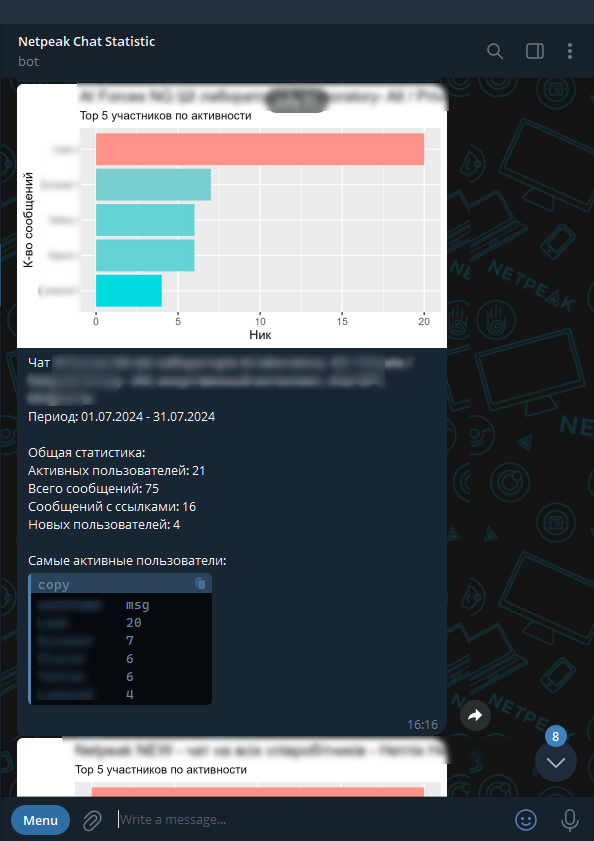
\includegraphics{img/2-chatstat.png}

\begin{Shaded}
\begin{Highlighting}[]
\CommentTok{\# функция для перевода data.frame в telegram таблицу }
\NormalTok{to\_tg\_table }\OtherTok{\textless{}{-}} \ControlFlowTok{function}\NormalTok{( table, }\AttributeTok{align =} \ConstantTok{NULL}\NormalTok{, }\AttributeTok{indents =} \DecValTok{3}\NormalTok{, }\AttributeTok{parse\_mode =} \StringTok{\textquotesingle{}Markdown\textquotesingle{}}\NormalTok{ ) \{}
  
  \CommentTok{\# если выравнивание не задано то выравниваем по левому краю}
  \ControlFlowTok{if}\NormalTok{ ( }\FunctionTok{is.null}\NormalTok{(align) ) \{}
    
\NormalTok{    col\_num }\OtherTok{\textless{}{-}} \FunctionTok{length}\NormalTok{(table)}
\NormalTok{    align   }\OtherTok{\textless{}{-}} \FunctionTok{str\_c}\NormalTok{( }\FunctionTok{rep}\NormalTok{(}\StringTok{\textquotesingle{}l\textquotesingle{}}\NormalTok{, col\_num), }\AttributeTok{collapse =} \StringTok{\textquotesingle{}\textquotesingle{}}\NormalTok{ )}
    
\NormalTok{  \}}
  
  \CommentTok{\# проверяем правильно ли заданно выравнивание}
  \ControlFlowTok{if}\NormalTok{ ( }\FunctionTok{length}\NormalTok{(table) }\SpecialCharTok{!=} \FunctionTok{nchar}\NormalTok{(align) ) \{}
    
\NormalTok{    align }\OtherTok{\textless{}{-}} \ConstantTok{NULL}
    
\NormalTok{  \}}
  
  \CommentTok{\# новое выравнивание столбцов }
\NormalTok{  side }\OtherTok{\textless{}{-}} \FunctionTok{sapply}\NormalTok{(}\DecValTok{1}\SpecialCharTok{:}\FunctionTok{nchar}\NormalTok{(align), }
                 \ControlFlowTok{function}\NormalTok{(x) \{ }
\NormalTok{                   letter }\OtherTok{\textless{}{-}} \FunctionTok{substr}\NormalTok{(align, x, x)}
                   \ControlFlowTok{switch}\NormalTok{ (letter,}
                           \StringTok{\textquotesingle{}l\textquotesingle{}} \OtherTok{=} \StringTok{\textquotesingle{}right\textquotesingle{}}\NormalTok{,}
                           \StringTok{\textquotesingle{}r\textquotesingle{}} \OtherTok{=} \StringTok{\textquotesingle{}left\textquotesingle{}}\NormalTok{,}
                           \StringTok{\textquotesingle{}c\textquotesingle{}} \OtherTok{=} \StringTok{\textquotesingle{}both\textquotesingle{}}\NormalTok{,}
                           \StringTok{\textquotesingle{}left\textquotesingle{}}
\NormalTok{                   )}
\NormalTok{                 \})}
  
  \CommentTok{\# сохраняем имена}
\NormalTok{  t\_names      }\OtherTok{\textless{}{-}} \FunctionTok{names}\NormalTok{(table)}
  
  \CommentTok{\# вычисляем ширину столбцов}
\NormalTok{  names\_length }\OtherTok{\textless{}{-}} \FunctionTok{sapply}\NormalTok{(t\_names, nchar) }
\NormalTok{  value\_length }\OtherTok{\textless{}{-}} \FunctionTok{sapply}\NormalTok{(table, }\ControlFlowTok{function}\NormalTok{(x) }\FunctionTok{max}\NormalTok{(}\FunctionTok{nchar}\NormalTok{(}\FunctionTok{as.character}\NormalTok{(x))))}
\NormalTok{  max\_length   }\OtherTok{\textless{}{-}} \FunctionTok{ifelse}\NormalTok{(value\_length }\SpecialCharTok{\textgreater{}}\NormalTok{ names\_length, value\_length, names\_length)}
  
  \CommentTok{\# подгоняем размер имён столбцов под их ширину + указанное в indents к{-}во пробелов }
\NormalTok{  t\_names }\OtherTok{\textless{}{-}} \FunctionTok{mapply}\NormalTok{(str\_pad, }
                    \AttributeTok{string =}\NormalTok{ t\_names, }
                    \AttributeTok{width  =}\NormalTok{ max\_length }\SpecialCharTok{+}\NormalTok{ indents, }
                    \AttributeTok{side   =}\NormalTok{ side)}
  
  \CommentTok{\# объединяем названия столбцов}
\NormalTok{  str\_names }\OtherTok{\textless{}{-}} \FunctionTok{str\_c}\NormalTok{(t\_names, }\AttributeTok{collapse =} \StringTok{\textquotesingle{}\textquotesingle{}}\NormalTok{)}
  
  \CommentTok{\# аргументы для фукнции str\_pad}
\NormalTok{  rules }\OtherTok{\textless{}{-}} \FunctionTok{list}\NormalTok{(}\AttributeTok{string =}\NormalTok{ table, }\AttributeTok{width =}\NormalTok{ max\_length }\SpecialCharTok{+}\NormalTok{ indents, }\AttributeTok{side =}\NormalTok{ side)}
  
  \CommentTok{\# поочереди переводим каждый столбец к нужному виду}
\NormalTok{  t\_str }\OtherTok{\textless{}{-}}   \FunctionTok{pmap\_df}\NormalTok{( rules, str\_pad )}\SpecialCharTok{\%\textgreater{}\%}
    \FunctionTok{unite}\NormalTok{(}\StringTok{"data"}\NormalTok{, }\FunctionTok{everything}\NormalTok{(), }\AttributeTok{remove =} \ConstantTok{TRUE}\NormalTok{, }\AttributeTok{sep =} \StringTok{\textquotesingle{}\textquotesingle{}}\NormalTok{) }\SpecialCharTok{\%\textgreater{}\%}
    \FunctionTok{unlist}\NormalTok{(data) }\SpecialCharTok{\%\textgreater{}\%}
    \FunctionTok{str\_c}\NormalTok{(}\AttributeTok{collapse =} \StringTok{\textquotesingle{}}\SpecialCharTok{\textbackslash{}n}\StringTok{\textquotesingle{}}\NormalTok{) }
  
  \CommentTok{\# если таблица занимает более 4096 символов обрезаем её}
  \ControlFlowTok{if}\NormalTok{ ( }\FunctionTok{nchar}\NormalTok{(t\_str) }\SpecialCharTok{\textgreater{}=} \DecValTok{4021}\NormalTok{ ) \{}
    
    \FunctionTok{warning}\NormalTok{(}\StringTok{\textquotesingle{}Таблица составляет более 4096 символов!\textquotesingle{}}\NormalTok{)}
\NormalTok{    t\_str }\OtherTok{\textless{}{-}} \FunctionTok{substr}\NormalTok{(t\_str, }\DecValTok{1}\NormalTok{, }\DecValTok{4021}\NormalTok{)}
    
\NormalTok{  \}}
  
  \CommentTok{\# символы выделения блока кода согласно выбранной разметке}
\NormalTok{  code\_block }\OtherTok{\textless{}{-}} \ControlFlowTok{switch}\NormalTok{(parse\_mode, }
                       \StringTok{\textquotesingle{}Markdown\textquotesingle{}} \OtherTok{=} \FunctionTok{c}\NormalTok{(}\StringTok{\textquotesingle{}\textasciigrave{}\textasciigrave{}\textasciigrave{}\textquotesingle{}}\NormalTok{, }\StringTok{\textquotesingle{}\textasciigrave{}\textasciigrave{}\textasciigrave{}\textquotesingle{}}\NormalTok{),}
                       \StringTok{\textquotesingle{}HTML\textquotesingle{}} \OtherTok{=} \FunctionTok{c}\NormalTok{(}\StringTok{\textquotesingle{}\textless{}code\textgreater{}\textquotesingle{}}\NormalTok{, }\StringTok{\textquotesingle{}\textless{}/code\textgreater{}\textquotesingle{}}\NormalTok{))}
  
  \CommentTok{\# переводим в code}
\NormalTok{  res }\OtherTok{\textless{}{-}} \FunctionTok{str\_c}\NormalTok{(code\_block[}\DecValTok{1}\NormalTok{], str\_names, t\_str, code\_block[}\DecValTok{2}\NormalTok{], }\AttributeTok{sep =} \StringTok{\textquotesingle{}}\SpecialCharTok{\textbackslash{}n}\StringTok{\textquotesingle{}}\NormalTok{)}
  
  \FunctionTok{return}\NormalTok{(res)}
\NormalTok{\}}
\end{Highlighting}
\end{Shaded}

Эту функцию мы уже разбирали в первой главе книги.

\subsection{Код бота сбора статистики}\label{ux43aux43eux434-ux431ux43eux442ux430-ux441ux431ux43eux440ux430-ux441ux442ux430ux442ux438ux441ux442ux438ux43aux438}

С методами бота мы разобрались, ниже привожу пример кода самого бота. Не забудьте подставить имя своего бота в функцию \texttt{bot\_token()}, или замените её на токен вашего бота.

\begin{Shaded}
\begin{Highlighting}[]
\FunctionTok{Sys.setlocale}\NormalTok{(}\AttributeTok{locale =} \StringTok{\textquotesingle{}russian\textquotesingle{}}\NormalTok{)}

\FunctionTok{library}\NormalTok{(telegram.bot)}
\FunctionTok{library}\NormalTok{(RSQLite)}
\FunctionTok{library}\NormalTok{(purrr)}
\FunctionTok{library}\NormalTok{(stringr)}
\FunctionTok{library}\NormalTok{(dplyr)}
\FunctionTok{library}\NormalTok{(here)}
\FunctionTok{library}\NormalTok{(tidyr)}
\FunctionTok{library}\NormalTok{(timeperiodsR)}
\FunctionTok{library}\NormalTok{(ggplot2)}

\CommentTok{\# Переменные}
\NormalTok{db\_name        }\OtherTok{\textless{}{-}} \StringTok{\textquotesingle{}chatstat.db\textquotesingle{}}
\NormalTok{msg\_tbl        }\OtherTok{\textless{}{-}} \StringTok{\textquotesingle{}message\textquotesingle{}}
\NormalTok{new\_user\_tbl   }\OtherTok{\textless{}{-}} \StringTok{\textquotesingle{}new\_users\textquotesingle{}}
\NormalTok{bot\_start\_time }\OtherTok{\textless{}{-}} \FunctionTok{Sys.time}\NormalTok{()}

\CommentTok{\# Чтение методов бота из каталога R}
\NormalTok{funcs }\OtherTok{\textless{}{-}} \FunctionTok{dir}\NormalTok{(}\FunctionTok{here}\NormalTok{(}\StringTok{\textquotesingle{}R\textquotesingle{}}\NormalTok{))}
\FunctionTok{walk}\NormalTok{(}\FunctionTok{here}\NormalTok{(}\StringTok{"R"}\NormalTok{, funcs), source)}

\CommentTok{\# Инициализация бота}
\NormalTok{updater }\OtherTok{\textless{}{-}} \FunctionTok{Updater}\NormalTok{(}\FunctionTok{bot\_token}\NormalTok{(}\StringTok{"Chat stat bot"}\NormalTok{))}
\NormalTok{updater}\SpecialCharTok{$}\NormalTok{bot}\SpecialCharTok{$}\FunctionTok{clean\_updates}\NormalTok{()}

\CommentTok{\# фильтры}
\CommentTok{\# фильтр для обработки сообщений msg}
\NormalTok{MessageFilters}\SpecialCharTok{$}\NormalTok{save\_msg }\OtherTok{\textless{}{-}} \FunctionTok{BaseFilter}\NormalTok{(}\ControlFlowTok{function}\NormalTok{(message) \{}
  
  \ControlFlowTok{if}\NormalTok{ ( }\SpecialCharTok{!}\FunctionTok{is.null}\NormalTok{(message}\SpecialCharTok{$}\NormalTok{text) ) \{}
    \ConstantTok{TRUE}
\NormalTok{  \} }\ControlFlowTok{else}\NormalTok{ \{}
    \ConstantTok{FALSE}
\NormalTok{  \}}
\NormalTok{\}}

\NormalTok{)}

\CommentTok{\# фильтр для обработки добавленных в чат участников}
\NormalTok{MessageFilters}\SpecialCharTok{$}\NormalTok{new\_users }\OtherTok{\textless{}{-}} \FunctionTok{BaseFilter}\NormalTok{(}\ControlFlowTok{function}\NormalTok{(message) \{}
  
  \ControlFlowTok{if}\NormalTok{ ( }\SpecialCharTok{!}\FunctionTok{is.null}\NormalTok{(message}\SpecialCharTok{$}\NormalTok{new\_chat\_member) ) \{}
    \ConstantTok{TRUE}
\NormalTok{  \} }\ControlFlowTok{else}\NormalTok{ \{}
    \ConstantTok{FALSE}
\NormalTok{  \}}
\NormalTok{\}}

\NormalTok{)}

\CommentTok{\# обработчики}
\NormalTok{h\_save\_msg }\OtherTok{\textless{}{-}} \FunctionTok{MessageHandler}\NormalTok{(get\_message, MessageFilters}\SpecialCharTok{$}\NormalTok{save\_msg }\SpecialCharTok{\&} \SpecialCharTok{!}\NormalTok{ MessageFilters}\SpecialCharTok{$}\NormalTok{command)}
\NormalTok{h\_new\_user }\OtherTok{\textless{}{-}} \FunctionTok{MessageHandler}\NormalTok{(get\_new\_user, MessageFilters}\SpecialCharTok{$}\NormalTok{new\_users }\SpecialCharTok{\&} \SpecialCharTok{!}\NormalTok{ MessageFilters}\SpecialCharTok{$}\NormalTok{command)}
\NormalTok{h\_stat     }\OtherTok{\textless{}{-}} \FunctionTok{CommandHandler}\NormalTok{(}\StringTok{\textquotesingle{}chat\_stat\textquotesingle{}}\NormalTok{, chat\_stat, }\AttributeTok{pass\_args =}\NormalTok{ T)}

\CommentTok{\# диспетчер}
\NormalTok{updater }\OtherTok{\textless{}{-}}
\NormalTok{  updater }\SpecialCharTok{+}
\NormalTok{  h\_save\_msg }\SpecialCharTok{+}
\NormalTok{  h\_new\_user }\SpecialCharTok{+}
\NormalTok{  h\_stat}

\CommentTok{\# запуск  бота}
\NormalTok{updater}\SpecialCharTok{$}\FunctionTok{start\_polling}\NormalTok{()}
\end{Highlighting}
\end{Shaded}

Далее добавляете созданного вами бота в ваши чаты, даёте ему права администратора, и он в фоновом режиме собирает статистику в свою внутреннюю базу. При необходимости можно использовать вместо SQLite какую то клиент серверную или облачную базу, в таком случае на основе собранной статистику без проблем вы сможете строить дашборды в различных BI системах.

Боты могут не только собирать статистику по активности в чатах, но так же модерировать их, считать карму её участников, отвечать на какие либо вопросы участников чата.

\section{Как добавить описание команд в интерфейс бота}\label{ux43aux430ux43a-ux434ux43eux431ux430ux432ux438ux442ux44c-ux43eux43fux438ux441ux430ux43dux438ux435-ux43aux43eux43cux430ux43dux434-ux432-ux438ux43dux442ux435ux440ux444ux435ux439ux441-ux431ux43eux442ux430}

Теперь вы умеете создавать полноценных ботов, которых помимо вас могут использовать другие пользователи. Но, для того, что бы облегчить поиск нужных команд вы можете добавить их в интефейс бота.

Выглядеть это будет вот так:
\includegraphics{http://img.netpeak.ua/alsey/160400158803_kiss_127kb.png}

Делается это через \href{@@BotFather}{BotFather} -\textgreater{} \texttt{@bot\_username} -\textgreater{} Edit Bot -\textgreater{} Edit Commands. Далее просто передаёте название команды и через тире их описание:

\begin{verbatim}
command1 - Description
command2 - Another description
\end{verbatim}

\section{Заключение}\label{ux437ux430ux43aux43bux44eux447ux435ux43dux438ux435-1}

Отличная работа! Вы освоили настройку команд и фильтров для вашего бота. Это основа для создания более сложных взаимодействий и функций. В следующей главе мы будем работать с клавиатурами --- как reply, так и inline, чтобы улучшить пользовательский интерфейс и взаимодействие с вашим ботом. Будьте готовы к тому, чтобы сделать ваш бот более интерактивным и удобным для пользователей.

\section{Тесты и задания}\label{ux442ux435ux441ux442ux44b-ux438-ux437ux430ux434ux430ux43dux438ux44f-1}

\subsection{Тесты}\label{ux442ux435ux441ux442ux44b-1}

Для закрепления материла рекомендую вам пройти тест доступный по \href{https://onlinetestpad.com/t/build-tg-bot-in-r-2}{ссылке}.

\subsection{Задания}\label{ux437ux430ux434ux430ux43dux438ux44f-1}

\begin{enumerate}
\def\labelenumi{\arabic{enumi}.}
\tightlist
\item
  Создайте бота, который будет по команде \texttt{/sum} и переданное в качестве дополнительных параметров произвольное количество перечисленных через пробел чисел, возвращать их сумму.
\end{enumerate}

Если вы всё сделали правильно результат должен быть таким:
\includegraphics{http://img.netpeak.ua/alsey/160400138798_kiss_126kb.png}

\chapter{Как добавить боту поддержку клавиатуры}\label{ux43aux430ux43a-ux434ux43eux431ux430ux432ux438ux442ux44c-ux431ux43eux442ux443-ux43fux43eux434ux434ux435ux440ux436ux43aux443-ux43aux43bux430ux432ux438ux430ux442ux443ux440ux44b}

В этой главе мы познакомимся с важным аспектом разработки Telegram-ботов - добавлением поддержки клавиатуры для более удобного взаимодействия пользователей с ботом.

Из этой главы вы узнаете:

\begin{itemize}
\tightlist
\item
  О двух основных типах клавиатур в Telegram: Reply и Inline
\item
  Как создавать и настраивать Reply-клавиатуру под панелью ввода текста
\item
  Как реализовать Inline-клавиатуру, привязанную к конкретным сообщениям бота
\item
  Как обрабатывать нажатия на кнопки клавиатур с помощью пакета telegram.bot для R
\item
  Как структурировать код бота для работы с клавиатурами
\item
  Практические примеры реализации ботов с клавиатурами для различных задач
\end{itemize}

Я подробно разберу процесс создания обоих типов клавиатур, приведу примеры кода для реализации нескольких полезных ботов. Вы познакомитесь с ботом для экспресс-тестирования на COVID-19, ботом для получения информации о погоде и ботом для вывода списка свежих статей с Хабра.
Я дам детальные объяснения структуры кода, функций для создания кнопок и обработки нажатий, а также рекомендации по построению логики работы бота с клавиатурами.

Освоив материал этой главы, вы сможете значительно улучшить удобство использования своих Telegram-ботов, сделав взаимодействие с ними более простым и интуитивно понятным для пользователей.

\section{Видео урок по добавлению боту клавиатуры}\label{ux432ux438ux434ux435ux43e-ux443ux440ux43eux43a-ux43fux43e-ux434ux43eux431ux430ux432ux43bux435ux43dux438ux44e-ux431ux43eux442ux443-ux43aux43bux430ux432ux438ux430ux442ux443ux440ux44b}

\section{Какие типы клавиатур поддерживает телеграм бот}\label{ux43aux430ux43aux438ux435-ux442ux438ux43fux44b-ux43aux43bux430ux432ux438ux430ux442ux443ux440-ux43fux43eux434ux434ux435ux440ux436ux438ux432ux430ux435ux442-ux442ux435ux43bux435ux433ux440ux430ux43c-ux431ux43eux442}

На момент написания книги \texttt{telegram.bot} позволяет вам создать клавиатуры двух типов:

\begin{itemize}
\tightlist
\item
  Reply - Основная, обычная клавиатура, которая находится под панелью ввода текста сообщения. Такая клавиатура просто отправляет боту текстовое сообщение, и в качестве текста отправит тот текст, который написан на самой кнопке.
\item
  Inline - Клавиатура привязанная к конкретному сообщению бота. Данная клавиатура отправляет боту данные, привязанные к нажатой кнопке, эти данные могут отличаться от текста, написанного на самой кнопке. И обрабатываются такие кнопки через \textbf{CallbackQueryHandler}.
\end{itemize}

Для того, что бы бот открыл клавиатуру необходимо при отправке сообщения через метод \texttt{sendMessage()}, передать созданную ранее клавиатуру в аргумент \texttt{reply\_markup}.

Ниже мы разберём несколько примеров.

\section{Reply клавиатура}\label{reply-ux43aux43bux430ux432ux438ux430ux442ux443ux440ux430}

Как я уже писал выше, это основная клавиатура управления ботом.

\begin{Shaded}
\begin{Highlighting}[]
\NormalTok{bot }\OtherTok{\textless{}{-}} \FunctionTok{Bot}\NormalTok{(}\AttributeTok{token =} \StringTok{"TOKEN"}\NormalTok{)}
\NormalTok{chat\_id }\OtherTok{\textless{}{-}} \StringTok{"CHAT\_ID"}

\CommentTok{\# Create Custom Keyboard}
\NormalTok{text }\OtherTok{\textless{}{-}} \StringTok{"Aren\textquotesingle{}t those custom keyboards cool?"}
\NormalTok{RKM }\OtherTok{\textless{}{-}} \FunctionTok{ReplyKeyboardMarkup}\NormalTok{(}
  \AttributeTok{keyboard =} \FunctionTok{list}\NormalTok{(}
    \FunctionTok{list}\NormalTok{(}\FunctionTok{KeyboardButton}\NormalTok{(}\StringTok{"Yes, they certainly are!"}\NormalTok{)),}
    \FunctionTok{list}\NormalTok{(}\FunctionTok{KeyboardButton}\NormalTok{(}\StringTok{"I\textquotesingle{}m not quite sure"}\NormalTok{)),}
    \FunctionTok{list}\NormalTok{(}\FunctionTok{KeyboardButton}\NormalTok{(}\StringTok{"No..."}\NormalTok{))}
\NormalTok{  ),}
  \AttributeTok{resize\_keyboard =} \ConstantTok{FALSE}\NormalTok{,}
  \AttributeTok{one\_time\_keyboard =} \ConstantTok{TRUE}
\NormalTok{)}

\CommentTok{\# Send Custom Keyboard}
\NormalTok{bot}\SpecialCharTok{$}\FunctionTok{sendMessage}\NormalTok{(chat\_id, text, }\AttributeTok{reply\_markup =}\NormalTok{ RKM)}
\end{Highlighting}
\end{Shaded}

Выше приведён пример из официальной справки пакета \texttt{telegram.bot}. Для создания клавиатуры используется функция \texttt{ReplyKeyboardMarkup()}, которая в свою очередь принимает список списков кнопок, которые создаются функцией \texttt{KeyboardButton()}.

Почему в \texttt{ReplyKeyboardMarkup()} необходимо передавать не просто список, а список списков? Дело в том, что вы передаёте основной список, и в нём отдельными списками вы задаёте каждый ряд кнопок, т.к. в один ряд можно расположить несколько кнопок.

Аргумент \texttt{resize\_keyboard} позволяет автоматически подбирать оптимальный размер кнопок клавиатуры, а аргумент \texttt{one\_time\_keyboard} позволяет скрывать клавиатуру после каждого нажатия на кнопку.

Давайте напишем простейшего бота, у которого будет 3 кнопки:
* Чат ID - Запросить чат ID диалога с ботом
* Моё имя - Запросить своё имя
* Мой логин - Запросить своё имя пользователя в телеграм

\begin{Shaded}
\begin{Highlighting}[]
\FunctionTok{library}\NormalTok{(telegram.bot)}

\CommentTok{\# создаём экземпляр класса Updater}
\NormalTok{updater }\OtherTok{\textless{}{-}} \FunctionTok{Updater}\NormalTok{(}\StringTok{\textquotesingle{}ТОКЕН ВАШЕГО БОТА\textquotesingle{}}\NormalTok{)}

\CommentTok{\# создаём методы}
\DocumentationTok{\#\# метод для запуска клавиатуры}
\NormalTok{start }\OtherTok{\textless{}{-}} \ControlFlowTok{function}\NormalTok{(bot, update) \{}

  \CommentTok{\# создаём клавиатуру}
\NormalTok{  RKM }\OtherTok{\textless{}{-}} \FunctionTok{ReplyKeyboardMarkup}\NormalTok{(}
    \AttributeTok{keyboard =} \FunctionTok{list}\NormalTok{(}
      \FunctionTok{list}\NormalTok{(}\FunctionTok{KeyboardButton}\NormalTok{(}\StringTok{"Чат ID"}\NormalTok{)),}
      \FunctionTok{list}\NormalTok{(}\FunctionTok{KeyboardButton}\NormalTok{(}\StringTok{"Моё имя"}\NormalTok{)),}
      \FunctionTok{list}\NormalTok{(}\FunctionTok{KeyboardButton}\NormalTok{(}\StringTok{"Мой логин"}\NormalTok{))}
\NormalTok{    ),}
    \AttributeTok{resize\_keyboard =} \ConstantTok{FALSE}\NormalTok{,}
    \AttributeTok{one\_time\_keyboard =} \ConstantTok{TRUE}
\NormalTok{  )}

  \CommentTok{\# отправляем клавиатуру}
\NormalTok{  bot}\SpecialCharTok{$}\FunctionTok{sendMessage}\NormalTok{(update}\SpecialCharTok{$}\FunctionTok{from\_chat\_id}\NormalTok{(),}
                  \AttributeTok{text =} \StringTok{\textquotesingle{}Выберите команду\textquotesingle{}}\NormalTok{,}
                  \AttributeTok{reply\_markup =}\NormalTok{ RKM)}

\NormalTok{\}}

\DocumentationTok{\#\# метод возвразающий id чата}
\NormalTok{chat\_id }\OtherTok{\textless{}{-}} \ControlFlowTok{function}\NormalTok{(bot, update) \{}

\NormalTok{  bot}\SpecialCharTok{$}\FunctionTok{sendMessage}\NormalTok{(update}\SpecialCharTok{$}\FunctionTok{from\_chat\_id}\NormalTok{(),}
                  \AttributeTok{text =} \FunctionTok{paste0}\NormalTok{(}\StringTok{"Чат id этого диалога: "}\NormalTok{, update}\SpecialCharTok{$}\FunctionTok{from\_chat\_id}\NormalTok{()),}
                  \AttributeTok{parse\_mode =} \StringTok{"Markdown"}\NormalTok{)}

\NormalTok{\}}

\DocumentationTok{\#\# метод возвращающий имя}
\NormalTok{my\_name }\OtherTok{\textless{}{-}} \ControlFlowTok{function}\NormalTok{(bot, update) \{}

\NormalTok{  bot}\SpecialCharTok{$}\FunctionTok{sendMessage}\NormalTok{(update}\SpecialCharTok{$}\FunctionTok{from\_chat\_id}\NormalTok{(),}
                  \AttributeTok{text =} \FunctionTok{paste0}\NormalTok{(}\StringTok{"Вас зовут "}\NormalTok{, update}\SpecialCharTok{$}\FunctionTok{effective\_user}\NormalTok{()}\SpecialCharTok{$}\NormalTok{first\_name),}
                  \AttributeTok{parse\_mode =} \StringTok{"Markdown"}\NormalTok{)}

\NormalTok{\}}

\DocumentationTok{\#\# метод возвращающий логин}
\NormalTok{my\_username }\OtherTok{\textless{}{-}} \ControlFlowTok{function}\NormalTok{(bot, update) \{}

\NormalTok{  bot}\SpecialCharTok{$}\FunctionTok{sendMessage}\NormalTok{(update}\SpecialCharTok{$}\FunctionTok{from\_chat\_id}\NormalTok{(),}
                  \AttributeTok{text =} \FunctionTok{paste0}\NormalTok{(}\StringTok{"Ваш логин "}\NormalTok{, update}\SpecialCharTok{$}\FunctionTok{effective\_user}\NormalTok{()}\SpecialCharTok{$}\NormalTok{username),}
                  \AttributeTok{parse\_mode =} \StringTok{"Markdown"}\NormalTok{)}

\NormalTok{\}}

\CommentTok{\# создаём фильтры}
\DocumentationTok{\#\# сообщения с текстом Чат ID}
\NormalTok{MessageFilters}\SpecialCharTok{$}\NormalTok{chat\_id }\OtherTok{\textless{}{-}} \FunctionTok{BaseFilter}\NormalTok{(}\ControlFlowTok{function}\NormalTok{(message) \{}

  \CommentTok{\# проверяем текст сообщения}
\NormalTok{  message}\SpecialCharTok{$}\NormalTok{text }\SpecialCharTok{==} \StringTok{"Чат ID"}

\NormalTok{\}}
\NormalTok{)}

\DocumentationTok{\#\# сообщения с текстом Моё имя}
\NormalTok{MessageFilters}\SpecialCharTok{$}\NormalTok{name }\OtherTok{\textless{}{-}} \FunctionTok{BaseFilter}\NormalTok{(}\ControlFlowTok{function}\NormalTok{(message) \{}

  \CommentTok{\# проверяем текст сообщения}
\NormalTok{  message}\SpecialCharTok{$}\NormalTok{text }\SpecialCharTok{==} \StringTok{"Моё имя"}

\NormalTok{\}}
\NormalTok{)}

\DocumentationTok{\#\# сообщения с текстом Мой логин}
\NormalTok{MessageFilters}\SpecialCharTok{$}\NormalTok{username }\OtherTok{\textless{}{-}} \FunctionTok{BaseFilter}\NormalTok{(}\ControlFlowTok{function}\NormalTok{(message) \{}

  \CommentTok{\# проверяем текст сообщения}
\NormalTok{  message}\SpecialCharTok{$}\NormalTok{text }\SpecialCharTok{==} \StringTok{"Мой логин"}
\ErrorTok{)}

\CommentTok{\# создаём обработчики}
\NormalTok{h\_start    }\OtherTok{\textless{}{-}} \FunctionTok{CommandHandler}\NormalTok{(}\StringTok{\textquotesingle{}start\textquotesingle{}}\NormalTok{, start)}
\NormalTok{h\_chat\_id  }\OtherTok{\textless{}{-}} \FunctionTok{MessageHandler}\NormalTok{(chat\_id, }\AttributeTok{filters =}\NormalTok{ MessageFilters}\SpecialCharTok{$}\NormalTok{chat\_id)}
\NormalTok{h\_name     }\OtherTok{\textless{}{-}} \FunctionTok{MessageHandler}\NormalTok{(my\_name, }\AttributeTok{filters =}\NormalTok{ MessageFilters}\SpecialCharTok{$}\NormalTok{name)}
\NormalTok{h\_username }\OtherTok{\textless{}{-}} \FunctionTok{MessageHandler}\NormalTok{(my\_username, }\AttributeTok{filters =}\NormalTok{ MessageFilters}\SpecialCharTok{$}\NormalTok{username)}

\CommentTok{\# добавляем обработчики в диспетчер}
\NormalTok{updater }\OtherTok{\textless{}{-}}\NormalTok{ updater }\SpecialCharTok{+}
\NormalTok{            h\_start }\SpecialCharTok{+}
\NormalTok{            h\_chat\_id }\SpecialCharTok{+}
\NormalTok{            h\_name }\SpecialCharTok{+}
\NormalTok{            h\_username}

\CommentTok{\# запускаем бота}
\NormalTok{updater}\SpecialCharTok{$}\FunctionTok{start\_polling}\NormalTok{()}
\end{Highlighting}
\end{Shaded}

\begin{quote}
Запустите приведённый выше пример кода, предварительно заменив `ТОКЕН ВАШЕГО БОТА' на реальный токен, который вы получили при создании бота через \emph{BotFather}.
\end{quote}

После запуска задайте боту команду \texttt{/start}, т.к. именно её мы определили для запуска клавиатуры.

\includegraphics{https://img.netpeak.ua/alsey/159860932526_kiss_163kb.png}

Если на данный момент вам сложно разобрать приведённый пример кода, с созданием методов, фильтров и обработчиков, то следует вернуться к предыдущей главе, в которой я подробно всё это описал.

Мы создали 4 метода:

\begin{itemize}
\tightlist
\item
  start - Запуск клавиатуры
\item
  chat\_id - Запрос идентификатора чата
\item
  my\_name - Запрос своего имени
\item
  my\_username - Запрос своего логина
\end{itemize}

В объект \emph{MessageFilters} добавили 3 фильтра сообщений, по их тексту:

\begin{itemize}
\tightlist
\item
  chat\_id - Сообщения с текстом \texttt{"Чат\ ID"}
\item
  name - Сообщения с текстом \texttt{"Моё\ имя"}
\item
  username - Сообщения с текстом \texttt{"Мой\ логин"}
\end{itemize}

И создали 4 обработчика, которые по заданным командам и фильтрам будут выполнять указанные методы.

\begin{Shaded}
\begin{Highlighting}[]
\CommentTok{\# создаём обработчики}
\NormalTok{h\_start    }\OtherTok{\textless{}{-}} \FunctionTok{CommandHandler}\NormalTok{(}\StringTok{\textquotesingle{}start\textquotesingle{}}\NormalTok{, start)}
\NormalTok{h\_chat\_id  }\OtherTok{\textless{}{-}} \FunctionTok{MessageHandler}\NormalTok{(chat\_id, }\AttributeTok{filters =}\NormalTok{ MessageFilters}\SpecialCharTok{$}\NormalTok{chat\_id)}
\NormalTok{h\_name     }\OtherTok{\textless{}{-}} \FunctionTok{MessageHandler}\NormalTok{(my\_name, }\AttributeTok{filters =}\NormalTok{ MessageFilters}\SpecialCharTok{$}\NormalTok{name)}
\NormalTok{h\_username }\OtherTok{\textless{}{-}} \FunctionTok{MessageHandler}\NormalTok{(my\_username, }\AttributeTok{filters =}\NormalTok{ MessageFilters}\SpecialCharTok{$}\NormalTok{username)}
\end{Highlighting}
\end{Shaded}

Сама клавиатура создаётся внутри метода \texttt{start()} командой \texttt{ReplyKeyboardMarkup()}.

\begin{Shaded}
\begin{Highlighting}[]
\NormalTok{RKM }\OtherTok{\textless{}{-}} \FunctionTok{ReplyKeyboardMarkup}\NormalTok{(}
    \AttributeTok{keyboard =} \FunctionTok{list}\NormalTok{(}
      \FunctionTok{list}\NormalTok{(}\FunctionTok{KeyboardButton}\NormalTok{(}\StringTok{"Чат ID"}\NormalTok{)),}
      \FunctionTok{list}\NormalTok{(}\FunctionTok{KeyboardButton}\NormalTok{(}\StringTok{"Моё имя"}\NormalTok{)),}
      \FunctionTok{list}\NormalTok{(}\FunctionTok{KeyboardButton}\NormalTok{(}\StringTok{"Мой логин"}\NormalTok{))}
\NormalTok{    ),}
    \AttributeTok{resize\_keyboard =} \ConstantTok{FALSE}\NormalTok{,}
    \AttributeTok{one\_time\_keyboard =} \ConstantTok{TRUE}
\NormalTok{)}
\end{Highlighting}
\end{Shaded}

В нашем случае все кнопки мы расположили друг под другом, но мы можем расположить их в один ряд, внеся изменения в список списков кнопок. Т.к. один ряд внутри клавиатуры создаётся через вложенный список кнопок, то для того, что бы вывести наши кнопки в один ряд надо переписать часть кода по построению клавиатуры вот так:

\begin{Shaded}
\begin{Highlighting}[]
\NormalTok{RKM }\OtherTok{\textless{}{-}} \FunctionTok{ReplyKeyboardMarkup}\NormalTok{(}
    \AttributeTok{keyboard =} \FunctionTok{list}\NormalTok{(}
      \FunctionTok{list}\NormalTok{(}
          \FunctionTok{KeyboardButton}\NormalTok{(}\StringTok{"Чат ID"}\NormalTok{),}
          \FunctionTok{KeyboardButton}\NormalTok{(}\StringTok{"Моё имя"}\NormalTok{),}
          \FunctionTok{KeyboardButton}\NormalTok{(}\StringTok{"Мой логин"}\NormalTok{)}
\NormalTok{     )}
\NormalTok{    ),}
    \AttributeTok{resize\_keyboard =} \ConstantTok{FALSE}\NormalTok{,}
    \AttributeTok{one\_time\_keyboard =} \ConstantTok{TRUE}
\NormalTok{)}
\end{Highlighting}
\end{Shaded}

\includegraphics{http://img.netpeak.ua/alsey/159861075655_kiss_153kb.png}

Отправляется клавиатура в чат методом \texttt{sendMessage()}, в аргументе \texttt{reply\_markup}.

\begin{Shaded}
\begin{Highlighting}[]
\NormalTok{  bot}\SpecialCharTok{$}\FunctionTok{sendMessage}\NormalTok{(update}\SpecialCharTok{$}\FunctionTok{from\_chat\_id}\NormalTok{(),}
                  \AttributeTok{text =} \StringTok{\textquotesingle{}Выберите команду\textquotesingle{}}\NormalTok{,}
                  \AttributeTok{reply\_markup =}\NormalTok{ RKM)}
\end{Highlighting}
\end{Shaded}

\subsection{Как запросить у пользователя номер телефона и локацию}\label{ux43aux430ux43a-ux437ux430ux43fux440ux43eux441ux438ux442ux44c-ux443-ux43fux43eux43bux44cux437ux43eux432ux430ux442ux435ux43bux44f-ux43dux43eux43cux435ux440-ux442ux435ux43bux435ux444ux43eux43dux430-ux438-ux43bux43eux43aux430ux446ux438ux44e}

При создании кнопок Reply клавиатуры мы используем функцию \texttt{KeyboardButton()}, у которой доступны 2 дополнительные аргумента:

\begin{itemize}
\tightlist
\item
  \texttt{request\_contact} - Запросить номер телефона пользователя
\item
  \texttt{request\_location} - Запросить локацию пользователя
\end{itemize}

\begin{Shaded}
\begin{Highlighting}[]
\NormalTok{bot }\OtherTok{\textless{}{-}} \FunctionTok{Bot}\NormalTok{(}\AttributeTok{token =} \StringTok{"ТОКЕН ВАШЕГО БОТА"}\NormalTok{)}

\NormalTok{chat\_id }\OtherTok{\textless{}{-}} \StringTok{"ID ВАШЕГО ЧАТА"}

\CommentTok{\# Create Custom Keyboard}
\NormalTok{text }\OtherTok{\textless{}{-}} \StringTok{"Поделитесь своими данными"}

\NormalTok{RKM }\OtherTok{\textless{}{-}} \FunctionTok{ReplyKeyboardMarkup}\NormalTok{(}
  \AttributeTok{keyboard =} \FunctionTok{list}\NormalTok{(}
    \FunctionTok{list}\NormalTok{(}\FunctionTok{KeyboardButton}\NormalTok{(}\StringTok{"Поделиться номером телефона"}\NormalTok{, }\AttributeTok{request\_contact =} \ConstantTok{TRUE}\NormalTok{)),}
    \FunctionTok{list}\NormalTok{(}\FunctionTok{KeyboardButton}\NormalTok{(}\StringTok{"Поделиться местонахождением"}\NormalTok{, }\AttributeTok{request\_location =} \ConstantTok{TRUE}\NormalTok{))}
\NormalTok{  ),}
  \AttributeTok{resize\_keyboard =} \ConstantTok{FALSE}\NormalTok{,}
  \AttributeTok{one\_time\_keyboard =} \ConstantTok{TRUE}
\NormalTok{)}

\CommentTok{\# Send Custom Keyboard}
\NormalTok{bot}\SpecialCharTok{$}\FunctionTok{sendMessage}\NormalTok{(chat\_id, text, }\AttributeTok{reply\_markup =}\NormalTok{ RKM)}
\end{Highlighting}
\end{Shaded}

Когда пользователь поделиться с ботом контактами, то в принятом от бота обновлении, в сообщении будет раздел \texttt{contact} со следующими данными:

\begin{itemize}
\tightlist
\item
  phone\_number - номер телефона в международном формате
\item
  first\_name - Имя
\item
  last\_name - Фамилия
\item
  user\_id - Внутренний идентификатор пользователя в telegram
\end{itemize}

Когда пользователь делиться местонахождением то в сообщении полученного ответа будет раздел \texttt{location} с информацией о координатах местонахождения пользователя, т.е. широта и долгота.

\section{Inline клавиатура}\label{inline-ux43aux43bux430ux432ux438ux430ux442ux443ux440ux430}

Как я уже писал выше, Inline клавиатура привязана к конкретному сообщению. С ней работать несколько сложнее чем с основной клавиатурой.

Изначально вам необходимо добавить боту метод, для вызова Inline клавиатуры.

Для ответа на нажатие Inline кнопки также можно использовать метод бота \texttt{answerCallbackQuery()}, который может вывести уведомление в интерфейсе telegram, пользователю нажавшему Inline кнопку.

Данные отправленные с Inline кнопки не являются текстом, поэтому для их обработки необходимо создать специальный обработчик с помощью команды \texttt{CallbackQueryHandler()}.

Код построения Inline клавиатуры который приводится в официальной справке пакета \texttt{telegram.bot}.

\begin{Shaded}
\begin{Highlighting}[]
\CommentTok{\# Initialize bot}
\NormalTok{bot }\OtherTok{\textless{}{-}} \FunctionTok{Bot}\NormalTok{(}\AttributeTok{token =} \StringTok{"TOKEN"}\NormalTok{)}
\NormalTok{chat\_id }\OtherTok{\textless{}{-}} \StringTok{"CHAT\_ID"}

\CommentTok{\# Create Inline Keyboard}
\NormalTok{text }\OtherTok{\textless{}{-}} \StringTok{"Could you type their phone number, please?"}
\NormalTok{IKM }\OtherTok{\textless{}{-}} \FunctionTok{InlineKeyboardMarkup}\NormalTok{(}
  \AttributeTok{inline\_keyboard =} \FunctionTok{list}\NormalTok{(}
    \FunctionTok{list}\NormalTok{(}
      \FunctionTok{InlineKeyboardButton}\NormalTok{(}\DecValTok{1}\NormalTok{),}
      \FunctionTok{InlineKeyboardButton}\NormalTok{(}\DecValTok{2}\NormalTok{),}
      \FunctionTok{InlineKeyboardButton}\NormalTok{(}\DecValTok{3}\NormalTok{)}
\NormalTok{    ),}
    \FunctionTok{list}\NormalTok{(}
      \FunctionTok{InlineKeyboardButton}\NormalTok{(}\DecValTok{4}\NormalTok{),}
      \FunctionTok{InlineKeyboardButton}\NormalTok{(}\DecValTok{5}\NormalTok{),}
      \FunctionTok{InlineKeyboardButton}\NormalTok{(}\DecValTok{6}\NormalTok{)}
\NormalTok{    ),}
    \FunctionTok{list}\NormalTok{(}
      \FunctionTok{InlineKeyboardButton}\NormalTok{(}\DecValTok{7}\NormalTok{),}
      \FunctionTok{InlineKeyboardButton}\NormalTok{(}\DecValTok{8}\NormalTok{),}
      \FunctionTok{InlineKeyboardButton}\NormalTok{(}\DecValTok{9}\NormalTok{)}
\NormalTok{    ),}
    \FunctionTok{list}\NormalTok{(}
      \FunctionTok{InlineKeyboardButton}\NormalTok{(}\StringTok{"*"}\NormalTok{),}
      \FunctionTok{InlineKeyboardButton}\NormalTok{(}\DecValTok{0}\NormalTok{),}
      \FunctionTok{InlineKeyboardButton}\NormalTok{(}\StringTok{"\#"}\NormalTok{)}
\NormalTok{    )}
\NormalTok{  )}
\NormalTok{)}

\CommentTok{\# Send Inline Keyboard}
\NormalTok{bot}\SpecialCharTok{$}\FunctionTok{sendMessage}\NormalTok{(chat\_id, text, }\AttributeTok{reply\_markup =}\NormalTok{ IKM)}
\end{Highlighting}
\end{Shaded}

Строить Inline клавиатуру необходимо с помощью команды \texttt{InlineKeyboardMarkup()}, по такому же принципу, как и Reply клавиатуру. В \texttt{InlineKeyboardMarkup()} необходимо передать список, списков Inline кнопок, каждая отдельная кнопка создаётся функцией \texttt{InlineKeyboardButton()}.

Inline кнопка может либо передавать боту какие-то данные с помощью аргумента \texttt{callback\_data}, либо открывать какую-либо HTML страницу, заданную с помощью аргумента \texttt{url}.

В результате будет список, в котором каждый элемент так же является списком Inline кнопок, которые необходимо объединить в один ряд.

Далее мы рассмотрим несколько примеров ботов с Inline кнопками.

\subsection{Пример простейшего бота с поддержкой InLine кнопок}\label{ux43fux440ux438ux43cux435ux440-ux43fux440ux43eux441ux442ux435ux439ux448ux435ux433ux43e-ux431ux43eux442ux430-ux441-ux43fux43eux434ux434ux435ux440ux436ux43aux43eux439-inline-ux43aux43dux43eux43fux43eux43a}

Для начала мы напишем бота для экспресс тестирования на covid-19. По команде \texttt{/test}, он будет отправлять вам клавиатуру с двумя кнопками, в зависимости от нажатой кнопки он будет присылать вам сообщение с результатами вашего тестирования.

\begin{Shaded}
\begin{Highlighting}[]
\FunctionTok{library}\NormalTok{(telegram.bot)}

\CommentTok{\# создаём экземпляр класса Updater}
\NormalTok{updater }\OtherTok{\textless{}{-}} \FunctionTok{Updater}\NormalTok{(}\StringTok{\textquotesingle{}ТОКЕН ВАШЕГО БОТА\textquotesingle{}}\NormalTok{)}

\CommentTok{\# метод для отправки InLine клавиатуры}
\NormalTok{test }\OtherTok{\textless{}{-}} \ControlFlowTok{function}\NormalTok{(bot, update) \{}


  \CommentTok{\# создаём InLine клавиатуру}
\NormalTok{  IKM }\OtherTok{\textless{}{-}} \FunctionTok{InlineKeyboardMarkup}\NormalTok{(}
    \AttributeTok{inline\_keyboard =} \FunctionTok{list}\NormalTok{(}
      \FunctionTok{list}\NormalTok{(}
        \FunctionTok{InlineKeyboardButton}\NormalTok{(}\StringTok{"Да"}\NormalTok{, }\AttributeTok{callback\_data =} \StringTok{\textquotesingle{}yes\textquotesingle{}}\NormalTok{),}
        \FunctionTok{InlineKeyboardButton}\NormalTok{(}\StringTok{"Нет"}\NormalTok{, }\AttributeTok{callback\_data =} \StringTok{\textquotesingle{}no\textquotesingle{}}\NormalTok{)}
\NormalTok{      )}
\NormalTok{    )}
\NormalTok{  )}

  \CommentTok{\# Отправляем клавиатуру в чат}
\NormalTok{  bot}\SpecialCharTok{$}\FunctionTok{sendMessage}\NormalTok{(update}\SpecialCharTok{$}\FunctionTok{from\_chat\_id}\NormalTok{(),}
                  \AttributeTok{text =} \StringTok{"Вы болете коронавирусом?"}\NormalTok{,}
                  \AttributeTok{reply\_markup =}\NormalTok{ IKM)}
\NormalTok{\}}

\CommentTok{\# метод для обработки нажатия кнопки}
\NormalTok{answer\_cb }\OtherTok{\textless{}{-}} \ControlFlowTok{function}\NormalTok{(bot, update) \{}

  \CommentTok{\# полученные данные с кнопки}
\NormalTok{  data }\OtherTok{\textless{}{-}}\NormalTok{ update}\SpecialCharTok{$}\NormalTok{callback\_query}\SpecialCharTok{$}\NormalTok{data}

  \CommentTok{\# получаем имя пользователя, нажавшего кнопку}
\NormalTok{  uname }\OtherTok{\textless{}{-}}\NormalTok{ update}\SpecialCharTok{$}\FunctionTok{effective\_user}\NormalTok{()}\SpecialCharTok{$}\NormalTok{first\_name}

  \CommentTok{\# обработка результата}
  \ControlFlowTok{if}\NormalTok{ ( data }\SpecialCharTok{==} \StringTok{\textquotesingle{}no\textquotesingle{}}\NormalTok{ ) \{}

\NormalTok{    msg }\OtherTok{\textless{}{-}} \FunctionTok{paste0}\NormalTok{(uname, }\StringTok{", поздравляю, ваш тест на covid{-}19 отрицательный."}\NormalTok{)}

\NormalTok{  \} }\ControlFlowTok{else}\NormalTok{ \{}

\NormalTok{    msg }\OtherTok{\textless{}{-}} \FunctionTok{paste0}\NormalTok{(uname, }\StringTok{", к сожалени ваш тест на covid{-}19 положительный."}\NormalTok{)}

\NormalTok{  \}}


  \CommentTok{\# Отправка сообщения}
\NormalTok{  bot}\SpecialCharTok{$}\FunctionTok{sendMessage}\NormalTok{(}\AttributeTok{chat\_id =}\NormalTok{ update}\SpecialCharTok{$}\FunctionTok{from\_chat\_id}\NormalTok{(),}
                  \AttributeTok{text =}\NormalTok{ msg)}

  \CommentTok{\# сообщаем боту, что запрос с кнопки принят}
\NormalTok{  bot}\SpecialCharTok{$}\FunctionTok{answerCallbackQuery}\NormalTok{(}\AttributeTok{callback\_query\_id =}\NormalTok{ update}\SpecialCharTok{$}\NormalTok{callback\_query}\SpecialCharTok{$}\NormalTok{id)}
\NormalTok{\}}

\CommentTok{\# создаём обработчики}
\NormalTok{inline\_h      }\OtherTok{\textless{}{-}} \FunctionTok{CommandHandler}\NormalTok{(}\StringTok{\textquotesingle{}test\textquotesingle{}}\NormalTok{, test)}
\NormalTok{query\_handler }\OtherTok{\textless{}{-}} \FunctionTok{CallbackQueryHandler}\NormalTok{(answer\_cb)}

\CommentTok{\# добавляем обработчики в диспетчер}
\NormalTok{updater }\OtherTok{\textless{}{-}}\NormalTok{ updater }\SpecialCharTok{+}\NormalTok{ inline\_h }\SpecialCharTok{+}\NormalTok{ query\_handler}

\CommentTok{\# запускаем бота}
\NormalTok{updater}\SpecialCharTok{$}\FunctionTok{start\_polling}\NormalTok{()}
\end{Highlighting}
\end{Shaded}

\begin{quote}
Запустите приведённый выше пример кода, предварительно заменив `ТОКЕН ВАШЕГО БОТА' на реальный токен, который вы получили при создании бота через \emph{BotFather}.
\end{quote}

Результат:
\includegraphics{https://img.netpeak.ua/alsey/159912494522_kiss_227kb.png}

Мы создали два метода:

\begin{itemize}
\tightlist
\item
  \emph{test} - Для отправки в чат Inline клавиатуры
\item
  \emph{answer\_cb} - Для обработки отправленных с клавиатуры данных.
\end{itemize}

Данные, которые будут отправлены с каждой кнопки задаются в аргументе \texttt{callback\_data}, при создании кнопки. Получить отправленные с кнопки данные можно с помощью конструкции \texttt{update\$callback\_query\$data}, внутри метода \emph{answer\_cb}.

Что бы бот реагировал на Inline клавиатуру, метод \emph{answer\_cb} обрабатывается специальным обработчиком: \texttt{CallbackQueryHandler(answer\_cb)}. Который запускает указанный метод по нажатию Inline кнопки. Обработчик \textbf{CallbackQueryHandler} принимает два аргумента:

\begin{itemize}
\tightlist
\item
  \texttt{callback} - Метод который необходимо запустить
\item
  \texttt{pattern} - Фильтр по данным, которые привязаны к кнопке с помощью аргумента \texttt{callback\_data}.
\end{itemize}

Соответвенно с помощью аргумента \texttt{pattern} мы можем под нажатие каждой кнопки написать отдельный метод:

\begin{Shaded}
\begin{Highlighting}[]
\FunctionTok{library}\NormalTok{(telegram.bot)}

\CommentTok{\# создаём экземпляр класса Updater}
\NormalTok{updater }\OtherTok{\textless{}{-}} \FunctionTok{Updater}\NormalTok{(}\StringTok{\textquotesingle{}ТОКЕН ВАШЕГО БОТА\textquotesingle{}}\NormalTok{)}

\CommentTok{\# метод для отправки InLine клавиатуры}
\NormalTok{test }\OtherTok{\textless{}{-}} \ControlFlowTok{function}\NormalTok{(bot, update) \{}

  \CommentTok{\# создаём InLine клавиатуру}
\NormalTok{  IKM }\OtherTok{\textless{}{-}} \FunctionTok{InlineKeyboardMarkup}\NormalTok{(}
    \AttributeTok{inline\_keyboard =} \FunctionTok{list}\NormalTok{(}
      \FunctionTok{list}\NormalTok{(}
        \FunctionTok{InlineKeyboardButton}\NormalTok{(}\StringTok{"Да"}\NormalTok{, }\AttributeTok{callback\_data =} \StringTok{\textquotesingle{}yes\textquotesingle{}}\NormalTok{),}
        \FunctionTok{InlineKeyboardButton}\NormalTok{(}\StringTok{"Нет"}\NormalTok{, }\AttributeTok{callback\_data =} \StringTok{\textquotesingle{}no\textquotesingle{}}\NormalTok{)}
\NormalTok{      )}
\NormalTok{    )}
\NormalTok{  )}

  \CommentTok{\# Отправляем клавиатуру в чат}
\NormalTok{  bot}\SpecialCharTok{$}\FunctionTok{sendMessage}\NormalTok{(update}\SpecialCharTok{$}\FunctionTok{from\_chat\_id}\NormalTok{(),}
                  \AttributeTok{text =} \StringTok{"Вы болете коронавирусом?"}\NormalTok{,}
                  \AttributeTok{reply\_markup =}\NormalTok{ IKM)}
\NormalTok{\}}

\CommentTok{\# метод для обработки нажатия кнопки Да}
\NormalTok{answer\_cb\_yes }\OtherTok{\textless{}{-}} \ControlFlowTok{function}\NormalTok{(bot, update) \{}

  \CommentTok{\# получаем имя пользователя, нажавшего кнопку}
\NormalTok{  uname }\OtherTok{\textless{}{-}}\NormalTok{ update}\SpecialCharTok{$}\FunctionTok{effective\_user}\NormalTok{()}\SpecialCharTok{$}\NormalTok{first\_name}

  \CommentTok{\# обработка результата}
\NormalTok{  msg }\OtherTok{\textless{}{-}} \FunctionTok{paste0}\NormalTok{(uname, }\StringTok{", к сожалени ваш текст на covid{-}19 положительный."}\NormalTok{)}

  \CommentTok{\# Отправка сообщения}
\NormalTok{  bot}\SpecialCharTok{$}\FunctionTok{sendMessage}\NormalTok{(}\AttributeTok{chat\_id =}\NormalTok{ update}\SpecialCharTok{$}\FunctionTok{from\_chat\_id}\NormalTok{(),}
                  \AttributeTok{text =}\NormalTok{ msg)}

  \CommentTok{\# сообщаем боту, что запрос с кнопки принят}
\NormalTok{  bot}\SpecialCharTok{$}\FunctionTok{answerCallbackQuery}\NormalTok{(}\AttributeTok{callback\_query\_id =}\NormalTok{ update}\SpecialCharTok{$}\NormalTok{callback\_query}\SpecialCharTok{$}\NormalTok{id)}
\NormalTok{\}}

\CommentTok{\# метод для обработки нажатия кнопки Нет}
\NormalTok{answer\_cb\_no }\OtherTok{\textless{}{-}} \ControlFlowTok{function}\NormalTok{(bot, update) \{}

  \CommentTok{\# получаем имя пользователя, нажавшего кнопку}
\NormalTok{  uname }\OtherTok{\textless{}{-}}\NormalTok{ update}\SpecialCharTok{$}\FunctionTok{effective\_user}\NormalTok{()}\SpecialCharTok{$}\NormalTok{first\_name}

\NormalTok{  msg }\OtherTok{\textless{}{-}} \FunctionTok{paste0}\NormalTok{(uname, }\StringTok{", поздравляю, ваш текст на covid{-}19 отрицательный."}\NormalTok{)}

  \CommentTok{\# Отправка сообщения}
\NormalTok{  bot}\SpecialCharTok{$}\FunctionTok{sendMessage}\NormalTok{(}\AttributeTok{chat\_id =}\NormalTok{ update}\SpecialCharTok{$}\FunctionTok{from\_chat\_id}\NormalTok{(),}
                  \AttributeTok{text =}\NormalTok{ msg)}

  \CommentTok{\# сообщаем боту, что запрос с кнопки принят}
\NormalTok{  bot}\SpecialCharTok{$}\FunctionTok{answerCallbackQuery}\NormalTok{(}\AttributeTok{callback\_query\_id =}\NormalTok{ update}\SpecialCharTok{$}\NormalTok{callback\_query}\SpecialCharTok{$}\NormalTok{id)}
\NormalTok{\}}

\CommentTok{\# создаём обработчики}
\NormalTok{inline\_h          }\OtherTok{\textless{}{-}} \FunctionTok{CommandHandler}\NormalTok{(}\StringTok{\textquotesingle{}test\textquotesingle{}}\NormalTok{, test)}
\NormalTok{query\_handler\_yes }\OtherTok{\textless{}{-}} \FunctionTok{CallbackQueryHandler}\NormalTok{(answer\_cb\_yes, }\AttributeTok{pattern =} \StringTok{\textquotesingle{}yes\textquotesingle{}}\NormalTok{)}
\NormalTok{query\_handler\_no  }\OtherTok{\textless{}{-}} \FunctionTok{CallbackQueryHandler}\NormalTok{(answer\_cb\_no, }\AttributeTok{pattern =} \StringTok{\textquotesingle{}no\textquotesingle{}}\NormalTok{)}

\CommentTok{\# добавляем обработчики в диспетчер}
\NormalTok{updater }\OtherTok{\textless{}{-}}\NormalTok{ updater }\SpecialCharTok{+}
\NormalTok{            inline\_h }\SpecialCharTok{+}
\NormalTok{            query\_handler\_yes }\SpecialCharTok{+}
\NormalTok{            query\_handler\_no}

\CommentTok{\# запускаем бота}
\NormalTok{updater}\SpecialCharTok{$}\FunctionTok{start\_polling}\NormalTok{()}
\end{Highlighting}
\end{Shaded}

\begin{quote}
Запустите приведённый выше пример кода, предварительно заменив `ТОКЕН ВАШЕГО БОТА' на реальный токен, который вы получили при создании бота через \emph{BotFather}.
\end{quote}

Теперь мы написали 2 отдельных метода, т.е. по одному методу, под нажатие каждой кнопки, и использовали аргумент \texttt{pattern}, при создании их обработчиков:

\begin{Shaded}
\begin{Highlighting}[]
\NormalTok{query\_handler\_yes }\OtherTok{\textless{}{-}} \FunctionTok{CallbackQueryHandler}\NormalTok{(answer\_cb\_yes, }\AttributeTok{pattern =} \StringTok{\textquotesingle{}yes\textquotesingle{}}\NormalTok{)}
\NormalTok{query\_handler\_no  }\OtherTok{\textless{}{-}} \FunctionTok{CallbackQueryHandler}\NormalTok{(answer\_cb\_no, }\AttributeTok{pattern =} \StringTok{\textquotesingle{}no\textquotesingle{}}\NormalTok{)}
\end{Highlighting}
\end{Shaded}

Заканчивается код метода \emph{answer\_cb} командой \texttt{bot\$answerCallbackQuery(callback\_query\_id\ =\ update\$callback\_query\$id)}, которая сообщает боту, что данные с inline клавиатуры получены.

\subsection{Пример бота, который сообщает текущую погоду по выбранному городу}\label{ux43fux440ux438ux43cux435ux440-ux431ux43eux442ux430-ux43aux43eux442ux43eux440ux44bux439-ux441ux43eux43eux431ux449ux430ux435ux442-ux442ux435ux43aux443ux449ux443ux44e-ux43fux43eux433ux43eux434ux443-ux43fux43e-ux432ux44bux431ux440ux430ux43dux43dux43eux43cux443-ux433ux43eux440ux43eux434ux443}

Давайте попробуем написать бота, который запрашивает данные о погоде.

Логика его работы будет следующая. Изначально командой \texttt{/start} вы вызываете основную клавиатуру, в которой присутствует всего одна кнопка ``Погода''. Нажав на эту кнопку вы получаете сообщение с Inline клавиатурой, для выбора города, по которому требуется узнать текущую погоду. Выбираете один из городов, и получаете текущую погоду.

В этом примере кода мы будем использовать несколько дополнительных пакетов:

\begin{itemize}
\tightlist
\item
  \texttt{httr} - пакет для работы с HTTP запросами, на основе которых построена работа с любым API. В нашем случае мы будем использовать бесплатный API \href{https://openweathermap.org/api}{openweathermap.org}.
\item
  \texttt{stringr} - пакет для работы с текстом, в нашем случае мы будем его использовать для формирования сообщения о погоде в выбранном городе.
\end{itemize}

\emph{Код бота, который сообщает текущую погоду по выбранному городу}

\begin{Shaded}
\begin{Highlighting}[]
\FunctionTok{library}\NormalTok{(telegram.bot)}
\FunctionTok{library}\NormalTok{(httr)}
\FunctionTok{library}\NormalTok{(stringr)}

\CommentTok{\# создаём экземпляр класса Updater}
\NormalTok{updater }\OtherTok{\textless{}{-}} \FunctionTok{Updater}\NormalTok{(}\StringTok{\textquotesingle{}ТОКЕН ВАШЕГО БОТА\textquotesingle{}}\NormalTok{)}

\CommentTok{\# создаём методы}
\DocumentationTok{\#\# метод для запуска основной клавиатуры}
\NormalTok{start }\OtherTok{\textless{}{-}} \ControlFlowTok{function}\NormalTok{(bot, update) \{}

  \CommentTok{\# создаём клавиатуру}
\NormalTok{  RKM }\OtherTok{\textless{}{-}} \FunctionTok{ReplyKeyboardMarkup}\NormalTok{(}
    \AttributeTok{keyboard =} \FunctionTok{list}\NormalTok{(}
      \FunctionTok{list}\NormalTok{(}
        \FunctionTok{KeyboardButton}\NormalTok{(}\StringTok{"Погода"}\NormalTok{)}
\NormalTok{      )}
\NormalTok{    ),}
    \AttributeTok{resize\_keyboard =} \ConstantTok{TRUE}\NormalTok{,}
    \AttributeTok{one\_time\_keyboard =} \ConstantTok{TRUE}
\NormalTok{  )}

  \CommentTok{\# отправляем клавиатуру}
\NormalTok{  bot}\SpecialCharTok{$}\FunctionTok{sendMessage}\NormalTok{(update}\SpecialCharTok{$}\FunctionTok{from\_chat\_id}\NormalTok{(),}
                  \AttributeTok{text =} \StringTok{\textquotesingle{}Выберите команду\textquotesingle{}}\NormalTok{,}
                  \AttributeTok{reply\_markup =}\NormalTok{ RKM)}

\NormalTok{\}}

\DocumentationTok{\#\# Метод вызова Inine клавиатуры}
\NormalTok{weather }\OtherTok{\textless{}{-}} \ControlFlowTok{function}\NormalTok{(bot, update) \{}

\NormalTok{  IKM }\OtherTok{\textless{}{-}} \FunctionTok{InlineKeyboardMarkup}\NormalTok{(}
    \AttributeTok{inline\_keyboard =} \FunctionTok{list}\NormalTok{(}
      \FunctionTok{list}\NormalTok{(}
        \FunctionTok{InlineKeyboardButton}\NormalTok{(}\AttributeTok{text =} \StringTok{\textquotesingle{}Москва\textquotesingle{}}\NormalTok{, }\AttributeTok{callback\_data =} \StringTok{\textquotesingle{}New York,us\textquotesingle{}}\NormalTok{),}
        \FunctionTok{InlineKeyboardButton}\NormalTok{(}\AttributeTok{text =} \StringTok{\textquotesingle{}Санкт{-}Петербург\textquotesingle{}}\NormalTok{, }\AttributeTok{callback\_data =} \StringTok{\textquotesingle{}Saint Petersburg\textquotesingle{}}\NormalTok{),}
        \FunctionTok{InlineKeyboardButton}\NormalTok{(}\AttributeTok{text =} \StringTok{\textquotesingle{}Нью{-}Йорк\textquotesingle{}}\NormalTok{, }\AttributeTok{callback\_data =} \StringTok{\textquotesingle{}New York\textquotesingle{}}\NormalTok{)}
\NormalTok{      ),}
      \FunctionTok{list}\NormalTok{(}
        \FunctionTok{InlineKeyboardButton}\NormalTok{(}\AttributeTok{text =} \StringTok{\textquotesingle{}Екатеринбург\textquotesingle{}}\NormalTok{, }\AttributeTok{callback\_data =} \StringTok{\textquotesingle{}Yekaterinburg,ru\textquotesingle{}}\NormalTok{),}
        \FunctionTok{InlineKeyboardButton}\NormalTok{(}\AttributeTok{text =} \StringTok{\textquotesingle{}Берлин\textquotesingle{}}\NormalTok{, }\AttributeTok{callback\_data =} \StringTok{\textquotesingle{}Berlin,de\textquotesingle{}}\NormalTok{),}
        \FunctionTok{InlineKeyboardButton}\NormalTok{(}\AttributeTok{text =} \StringTok{\textquotesingle{}Париж\textquotesingle{}}\NormalTok{, }\AttributeTok{callback\_data =} \StringTok{\textquotesingle{}Paris,fr\textquotesingle{}}\NormalTok{)}
\NormalTok{      ),}
      \FunctionTok{list}\NormalTok{(}
        \FunctionTok{InlineKeyboardButton}\NormalTok{(}\AttributeTok{text =} \StringTok{\textquotesingle{}Рим\textquotesingle{}}\NormalTok{, }\AttributeTok{callback\_data =} \StringTok{\textquotesingle{}Rome,it\textquotesingle{}}\NormalTok{),}
        \FunctionTok{InlineKeyboardButton}\NormalTok{(}\AttributeTok{text =} \StringTok{\textquotesingle{}Одесса\textquotesingle{}}\NormalTok{, }\AttributeTok{callback\_data =} \StringTok{\textquotesingle{}Odessa,ua\textquotesingle{}}\NormalTok{),}
        \FunctionTok{InlineKeyboardButton}\NormalTok{(}\AttributeTok{text =} \StringTok{\textquotesingle{}Киев\textquotesingle{}}\NormalTok{, }\AttributeTok{callback\_data =} \StringTok{\textquotesingle{}Kyiv,ua\textquotesingle{}}\NormalTok{)}
\NormalTok{      ),}
      \FunctionTok{list}\NormalTok{(}
        \FunctionTok{InlineKeyboardButton}\NormalTok{(}\AttributeTok{text =} \StringTok{\textquotesingle{}Токио\textquotesingle{}}\NormalTok{, }\AttributeTok{callback\_data =} \StringTok{\textquotesingle{}Tokyo\textquotesingle{}}\NormalTok{),}
        \FunctionTok{InlineKeyboardButton}\NormalTok{(}\AttributeTok{text =} \StringTok{\textquotesingle{}Амстердам\textquotesingle{}}\NormalTok{, }\AttributeTok{callback\_data =} \StringTok{\textquotesingle{}Amsterdam,nl\textquotesingle{}}\NormalTok{),}
        \FunctionTok{InlineKeyboardButton}\NormalTok{(}\AttributeTok{text =} \StringTok{\textquotesingle{}Вашингтон\textquotesingle{}}\NormalTok{, }\AttributeTok{callback\_data =} \StringTok{\textquotesingle{}Washington,us\textquotesingle{}}\NormalTok{)}
\NormalTok{      )}
\NormalTok{    )}
\NormalTok{  )}

  \CommentTok{\# Send Inline Keyboard}
\NormalTok{  bot}\SpecialCharTok{$}\FunctionTok{sendMessage}\NormalTok{(}\AttributeTok{chat\_id =}\NormalTok{ update}\SpecialCharTok{$}\FunctionTok{from\_chat\_id}\NormalTok{(),}
                  \AttributeTok{text =} \StringTok{"Выберите город"}\NormalTok{,}
                  \AttributeTok{reply\_markup =}\NormalTok{ IKM)}
\NormalTok{\}}

\CommentTok{\# метод для сообщения погоды}
\NormalTok{answer\_cb }\OtherTok{\textless{}{-}} \ControlFlowTok{function}\NormalTok{(bot, update) \{}

  \CommentTok{\# получаем из сообщения город}
\NormalTok{  city }\OtherTok{\textless{}{-}}\NormalTok{ update}\SpecialCharTok{$}\NormalTok{callback\_query}\SpecialCharTok{$}\NormalTok{data}

  \CommentTok{\# отправляем запрос}
\NormalTok{  ans }\OtherTok{\textless{}{-}} \FunctionTok{GET}\NormalTok{(}\StringTok{\textquotesingle{}https://api.openweathermap.org/data/2.5/weather\textquotesingle{}}\NormalTok{,}
             \AttributeTok{query =} \FunctionTok{list}\NormalTok{(}\AttributeTok{q     =}\NormalTok{ city,}
                          \AttributeTok{lang  =} \StringTok{\textquotesingle{}ru\textquotesingle{}}\NormalTok{,}
                          \AttributeTok{units =} \StringTok{\textquotesingle{}metric\textquotesingle{}}\NormalTok{,}
                          \AttributeTok{appid =} \StringTok{\textquotesingle{}4776568ccea136ffe4cda9f1969af340\textquotesingle{}}\NormalTok{))}

  \CommentTok{\# парсим ответ}
\NormalTok{  result }\OtherTok{\textless{}{-}} \FunctionTok{content}\NormalTok{(ans)}

  \CommentTok{\# формируем сообщение}
\NormalTok{  msg }\OtherTok{\textless{}{-}} \FunctionTok{str\_glue}\NormalTok{(}\StringTok{"\{result$name\} погода:}\SpecialCharTok{\textbackslash{}n}\StringTok{"}\NormalTok{,}
                  \StringTok{"Текущая температура: \{result$main$temp\}}\SpecialCharTok{\textbackslash{}n}\StringTok{"}\NormalTok{,}
                  \StringTok{"Скорость ветра: \{result$wind$speed\}}\SpecialCharTok{\textbackslash{}n}\StringTok{"}\NormalTok{,}
                  \StringTok{"Описание: \{result$weather[[1]]$description\}"}\NormalTok{)}

  \CommentTok{\# отправляем информацию о погоде}
\NormalTok{  bot}\SpecialCharTok{$}\FunctionTok{sendMessage}\NormalTok{(}\AttributeTok{chat\_id =}\NormalTok{ update}\SpecialCharTok{$}\FunctionTok{from\_chat\_id}\NormalTok{(),}
                  \AttributeTok{text    =}\NormalTok{ msg)}


\NormalTok{  bot}\SpecialCharTok{$}\FunctionTok{answerCallbackQuery}\NormalTok{(}\AttributeTok{callback\_query\_id =}\NormalTok{ update}\SpecialCharTok{$}\NormalTok{callback\_query}\SpecialCharTok{$}\NormalTok{id)}
\NormalTok{\}}

\CommentTok{\# создаём фильтры}
\DocumentationTok{\#\# сообщения с текстом Погода}
\NormalTok{MessageFilters}\SpecialCharTok{$}\NormalTok{weather }\OtherTok{\textless{}{-}} \FunctionTok{BaseFilter}\NormalTok{(}\ControlFlowTok{function}\NormalTok{(message) \{}

  \CommentTok{\# проверяем текст сообщения}
\NormalTok{  message}\SpecialCharTok{$}\NormalTok{text }\SpecialCharTok{==} \StringTok{"Погода"}

\NormalTok{\}}
\NormalTok{)}

\CommentTok{\# создаём обработчики}
\NormalTok{h\_start         }\OtherTok{\textless{}{-}} \FunctionTok{CommandHandler}\NormalTok{(}\StringTok{\textquotesingle{}start\textquotesingle{}}\NormalTok{, start)}
\NormalTok{h\_weather       }\OtherTok{\textless{}{-}} \FunctionTok{MessageHandler}\NormalTok{(weather, }\AttributeTok{filters =}\NormalTok{ MessageFilters}\SpecialCharTok{$}\NormalTok{weather)}
\NormalTok{h\_query\_handler }\OtherTok{\textless{}{-}} \FunctionTok{CallbackQueryHandler}\NormalTok{(answer\_cb)}

\CommentTok{\# добавляем обработчики в диспетчер}
\NormalTok{updater }\OtherTok{\textless{}{-}}\NormalTok{ updater }\SpecialCharTok{+}
\NormalTok{              h\_start }\SpecialCharTok{+}
\NormalTok{              h\_weather }\SpecialCharTok{+}
\NormalTok{              h\_query\_handler}

\CommentTok{\# запускаем бота}
\NormalTok{updater}\SpecialCharTok{$}\FunctionTok{start\_polling}\NormalTok{()}
\end{Highlighting}
\end{Shaded}

\begin{quote}
Запустите приведённый выше пример кода, предварительно заменив `ТОКЕН ВАШЕГО БОТА' на реальный токен, который вы получили при создании бота через \emph{BotFather}.
\end{quote}

В результате наш бот будет работать примерно так:
\includegraphics{https://img.netpeak.ua/alsey/159863902887_kiss_184kb.png}

Схематически данного бота можно изобрать вот так:
\includegraphics{http://img.netpeak.ua/alsey/159906484732_kiss_23kb.png}

Мы создали 3 метода, доступные внутри нашего погодного бота:

\begin{itemize}
\tightlist
\item
  \emph{start} - Запуск основной клавиатуры бота
\item
  \emph{weather} - Запуск Inline клавиатуры для выбора города
\item
  \emph{answer\_cb} - Основной метод, который по заданному городу запрашивает в API погоду, и отправляет её в чат.
\end{itemize}

Метод \emph{start} у нас запускается командой \texttt{/start}, что реализовано обработчиком \texttt{CommandHandler(\textquotesingle{}start\textquotesingle{},\ start)}.

Для запуска метода \emph{weather} мы создали одноимённый фильтр:

\begin{Shaded}
\begin{Highlighting}[]
\CommentTok{\# создаём фильтры}
\DocumentationTok{\#\# сообщения с текстом Погода}
\NormalTok{MessageFilters}\SpecialCharTok{$}\NormalTok{weather }\OtherTok{\textless{}{-}} \FunctionTok{BaseFilter}\NormalTok{(}\ControlFlowTok{function}\NormalTok{(message) \{}

  \CommentTok{\# проверяем текст сообщения}
\NormalTok{  message}\SpecialCharTok{$}\NormalTok{text }\SpecialCharTok{==} \StringTok{"Погода"}

\NormalTok{\}}
\NormalTok{)}
\end{Highlighting}
\end{Shaded}

И вызываем этот метод следующим обработчиком сообщений: \texttt{MessageHandler(weather,\ filters\ =\ MessageFilters\$weather)}.

И в конце концов, основной наш метод \emph{answer\_cb} реагирует на нажатие Inline кнопок, что реализовано специальным обработчиком: \texttt{CallbackQueryHandler(answer\_cb)}.

Внутри метода \emph{answer\_cb}, мы считываем отправленные с клавиатуры данные и записываем их в переменную \texttt{city}: \texttt{city\ \textless{}-\ update\$callback\_query\$data}. После чего запрашиваем из API данные о погоде, формируем и отправляем сообщение, и в конце концов используем метод \texttt{answerCallbackQuery} для того, что бы сообщить боту, о том, что мы обработали нажатие Inline кнопки.

\subsection{Пример бота, который выводит список самых свежих статей со ссылками по-указанному Хабу из habr.com}\label{ux43fux440ux438ux43cux435ux440-ux431ux43eux442ux430-ux43aux43eux442ux43eux440ux44bux439-ux432ux44bux432ux43eux434ux438ux442-ux441ux43fux438ux441ux43eux43a-ux441ux430ux43cux44bux445-ux441ux432ux435ux436ux438ux445-ux441ux442ux430ux442ux435ux439-ux441ux43e-ux441ux441ux44bux43bux43aux430ux43cux438-ux43fux43e-ux443ux43aux430ux437ux430ux43dux43dux43eux43cux443-ux445ux430ux431ux443-ux438ux437-habr.com}

Данного бота я привожу для того, что бы показать вам, как вывести Inline кнопки которые ведут на веб страницы.

Логика данного бота схожа с предыдущим, изначально мы запускаем основную клавиатуру командой \texttt{/start}. Далее бот даёт нам на выбор список из 6 хабов, мы выбираем интересующий нас хаб, и получаем 5 самых свежих публикаций из выбранного Хаба.

Как вы понимаете, в данном случае нам необходимо получить список статей, и для этого мы будем использовать пакет \texttt{tidyRSS}, который позволяет вам получать RSS feed (ленту) сайта в виде обычного дата фрейма в R, к счастью Хабр предоставляет RSS фид под каждый отдельный хаб.

\begin{quote}
RSS --- это файл в формате .XML или .RSS, который используют сайты, чтобы передавать пользователю информацию об обновлениях.
\end{quote}

Для начала установим пакет \texttt{tidyRSS}.

\begin{Shaded}
\begin{Highlighting}[]
\FunctionTok{install.packages}\NormalTok{(}\StringTok{\textquotesingle{}\textasciigrave{}tidyRSS\textasciigrave{}\textquotesingle{}}\NormalTok{)}
\end{Highlighting}
\end{Shaded}

Получить RRS Feed по какому то хабу можно примерно так:

\begin{Shaded}
\begin{Highlighting}[]
\FunctionTok{library}\NormalTok{(tidyRSS)}
\NormalTok{url }\OtherTok{\textless{}{-}} \StringTok{\textquotesingle{}https://habr.com/ru/rss/hub/r/\textquotesingle{}}
\NormalTok{rss\_fead }\OtherTok{\textless{}{-}} \FunctionTok{tidyfeed}\NormalTok{(url)}
\end{Highlighting}
\end{Shaded}

Теперь рассмотрим код построения описанного выше бота:

\emph{Код бот который выводит список наиболее свежих статей по выбранному Хабу}

\begin{Shaded}
\begin{Highlighting}[]
\FunctionTok{library}\NormalTok{(telegram.bot)}
\FunctionTok{library}\NormalTok{(tidyRSS)}

\CommentTok{\# создаём экземпляр класса Updater}
\NormalTok{updater }\OtherTok{\textless{}{-}} \FunctionTok{Updater}\NormalTok{(}\StringTok{\textquotesingle{}ТОКЕН ВАШЕГО БОТА\textquotesingle{}}\NormalTok{)}

\CommentTok{\# создаём методы}
\DocumentationTok{\#\# метод для запуска основной клавиатуры}
\NormalTok{start }\OtherTok{\textless{}{-}} \ControlFlowTok{function}\NormalTok{(bot, update) \{}
  
  \CommentTok{\# создаём клавиатуру}
\NormalTok{  RKM }\OtherTok{\textless{}{-}} \FunctionTok{ReplyKeyboardMarkup}\NormalTok{(}
    \AttributeTok{keyboard =} \FunctionTok{list}\NormalTok{(}
      \FunctionTok{list}\NormalTok{(}
        \FunctionTok{KeyboardButton}\NormalTok{(}\StringTok{"Список статей"}\NormalTok{)}
\NormalTok{      )}
\NormalTok{    ),}
    \AttributeTok{resize\_keyboard =} \ConstantTok{TRUE}\NormalTok{,}
    \AttributeTok{one\_time\_keyboard =} \ConstantTok{TRUE}
\NormalTok{  )}
  
  \CommentTok{\# отправляем клавиатуру}
\NormalTok{  bot}\SpecialCharTok{$}\FunctionTok{sendMessage}\NormalTok{(update}\SpecialCharTok{$}\FunctionTok{from\_chat\_id}\NormalTok{(),}
                  \AttributeTok{text =} \StringTok{\textquotesingle{}Выберите команду\textquotesingle{}}\NormalTok{,}
                  \AttributeTok{reply\_markup =}\NormalTok{ RKM)}
  
\NormalTok{\}}

\DocumentationTok{\#\# Метод вызова Inine клавиатуры}
\NormalTok{habs }\OtherTok{\textless{}{-}} \ControlFlowTok{function}\NormalTok{(bot, update) \{}
  
\NormalTok{  IKM }\OtherTok{\textless{}{-}} \FunctionTok{InlineKeyboardMarkup}\NormalTok{(}
    \AttributeTok{inline\_keyboard =} \FunctionTok{list}\NormalTok{(}
      \FunctionTok{list}\NormalTok{(}
        \FunctionTok{InlineKeyboardButton}\NormalTok{(}\AttributeTok{text =} \StringTok{\textquotesingle{}R\textquotesingle{}}\NormalTok{, }\AttributeTok{callback\_data =} \StringTok{\textquotesingle{}r\textquotesingle{}}\NormalTok{),}
        \FunctionTok{InlineKeyboardButton}\NormalTok{(}\AttributeTok{text =} \StringTok{\textquotesingle{}Data Mining\textquotesingle{}}\NormalTok{, }\AttributeTok{callback\_data =} \StringTok{\textquotesingle{}data\_mining\textquotesingle{}}\NormalTok{),}
        \FunctionTok{InlineKeyboardButton}\NormalTok{(}\AttributeTok{text =} \StringTok{\textquotesingle{}Data Engineering\textquotesingle{}}\NormalTok{, }\AttributeTok{callback\_data =} \StringTok{\textquotesingle{}data\_engineering\textquotesingle{}}\NormalTok{)}
\NormalTok{      ),}
      \FunctionTok{list}\NormalTok{(}
        \FunctionTok{InlineKeyboardButton}\NormalTok{(}\AttributeTok{text =} \StringTok{\textquotesingle{}Big Data\textquotesingle{}}\NormalTok{, }\AttributeTok{callback\_data =} \StringTok{\textquotesingle{}bigdata\textquotesingle{}}\NormalTok{),}
        \FunctionTok{InlineKeyboardButton}\NormalTok{(}\AttributeTok{text =} \StringTok{\textquotesingle{}Python\textquotesingle{}}\NormalTok{, }\AttributeTok{callback\_data =} \StringTok{\textquotesingle{}python\textquotesingle{}}\NormalTok{),}
        \FunctionTok{InlineKeyboardButton}\NormalTok{(}\AttributeTok{text =} \StringTok{\textquotesingle{}Визуализация данных\textquotesingle{}}\NormalTok{, }\AttributeTok{callback\_data =} \StringTok{\textquotesingle{}data\_visualization\textquotesingle{}}\NormalTok{)}
\NormalTok{      )}
\NormalTok{    )}
\NormalTok{  )}
  
  \CommentTok{\# Send Inline Keyboard}
\NormalTok{  bot}\SpecialCharTok{$}\FunctionTok{sendMessage}\NormalTok{(}\AttributeTok{chat\_id =}\NormalTok{ update}\SpecialCharTok{$}\FunctionTok{from\_chat\_id}\NormalTok{(),}
                  \AttributeTok{text =} \StringTok{"Выберите Хаб"}\NormalTok{,}
                  \AttributeTok{reply\_markup =}\NormalTok{ IKM)}
\NormalTok{\}}

\CommentTok{\# метод для сообщения погоды}
\NormalTok{answer\_cb }\OtherTok{\textless{}{-}} \ControlFlowTok{function}\NormalTok{(bot, update) \{}
  
  \CommentTok{\# получаем из сообщения название хаба}
\NormalTok{  hub }\OtherTok{\textless{}{-}}\NormalTok{ update}\SpecialCharTok{$}\NormalTok{callback\_query}\SpecialCharTok{$}\NormalTok{data}
  
  \CommentTok{\# сообщение о том, что данные по кнопке получены}
\NormalTok{  bot}\SpecialCharTok{$}\FunctionTok{answerCallbackQuery}\NormalTok{(}\AttributeTok{callback\_query\_id =}\NormalTok{ update}\SpecialCharTok{$}\NormalTok{callback\_query}\SpecialCharTok{$}\NormalTok{id,}
                          \AttributeTok{text =} \StringTok{\textquotesingle{}Подождите несколько минут, запрос обрабатывается\textquotesingle{}}\NormalTok{)}
  
  \CommentTok{\# сообщение о том, что надо подождать пока бот получит данные}
\NormalTok{  mid }\OtherTok{\textless{}{-}}\NormalTok{ bot}\SpecialCharTok{$}\FunctionTok{sendMessage}\NormalTok{(}\AttributeTok{chat\_id =}\NormalTok{ update}\SpecialCharTok{$}\FunctionTok{from\_chat\_id}\NormalTok{(),}
                         \AttributeTok{text    =} \StringTok{"Подождите несколько минут пока, я соберу данные по выбранному Хабу"}\NormalTok{)}
  
  \CommentTok{\# запрашиваем RSS Feed по Хабу}
\NormalTok{  url   }\OtherTok{\textless{}{-}} \FunctionTok{paste0}\NormalTok{(}\StringTok{\textquotesingle{}https://habr.com/ru/rss/hub/\textquotesingle{}}\NormalTok{, hub, }\StringTok{\textquotesingle{}/\textquotesingle{}}\NormalTok{)}
\NormalTok{  posts }\OtherTok{\textless{}{-}} \FunctionTok{head}\NormalTok{(}\FunctionTok{tidyfeed}\NormalTok{(url), }\DecValTok{5}\NormalTok{)}
  
  \CommentTok{\# удаляем сообщение о том, что надо подождать}
\NormalTok{  bot}\SpecialCharTok{$}\FunctionTok{deleteMessage}\NormalTok{(update}\SpecialCharTok{$}\FunctionTok{from\_chat\_id}\NormalTok{(), mid}\SpecialCharTok{$}\NormalTok{message\_id)}
  
  \CommentTok{\# формируем список кнопок}
\NormalTok{  keys }\OtherTok{\textless{}{-}} \FunctionTok{lapply}\NormalTok{(}\DecValTok{1}\SpecialCharTok{:}\DecValTok{5}\NormalTok{, }\ControlFlowTok{function}\NormalTok{(x) }\FunctionTok{list}\NormalTok{(}\FunctionTok{InlineKeyboardButton}\NormalTok{(posts}\SpecialCharTok{$}\NormalTok{item\_title[x], }\AttributeTok{url =}\NormalTok{ posts}\SpecialCharTok{$}\NormalTok{item\_link[x])))}
  
  \CommentTok{\# формируем клавиатуру}
\NormalTok{  IKM }\OtherTok{\textless{}{-}} \FunctionTok{InlineKeyboardMarkup}\NormalTok{(}
    \AttributeTok{inline\_keyboard =}\NormalTok{  keys}
\NormalTok{  )}
  
  \CommentTok{\# отправляем информацию о погоде}
\NormalTok{  bot}\SpecialCharTok{$}\FunctionTok{sendMessage}\NormalTok{(}\AttributeTok{chat\_id =}\NormalTok{ update}\SpecialCharTok{$}\FunctionTok{from\_chat\_id}\NormalTok{(),}
                  \AttributeTok{text    =} \FunctionTok{paste0}\NormalTok{(}\StringTok{"5 наиболее свежих статей из Хаба "}\NormalTok{, hub),}
                  \AttributeTok{reply\_markup =}\NormalTok{ IKM)}
  
\NormalTok{\}}

\CommentTok{\# создаём фильтры}
\DocumentationTok{\#\# сообщения с текстом Погода}
\NormalTok{MessageFilters}\SpecialCharTok{$}\NormalTok{hubs }\OtherTok{\textless{}{-}} \FunctionTok{BaseFilter}\NormalTok{(}\ControlFlowTok{function}\NormalTok{(message) \{}
  
  \CommentTok{\# проверяем текст сообщения}
\NormalTok{  message}\SpecialCharTok{$}\NormalTok{text }\SpecialCharTok{==} \StringTok{"Список статей"}
  
\NormalTok{\}}
\NormalTok{)}

\CommentTok{\# создаём обработчики}
\NormalTok{h\_start         }\OtherTok{\textless{}{-}} \FunctionTok{CommandHandler}\NormalTok{(}\StringTok{\textquotesingle{}start\textquotesingle{}}\NormalTok{, start)}
\NormalTok{h\_hubs          }\OtherTok{\textless{}{-}} \FunctionTok{MessageHandler}\NormalTok{(habs, }\AttributeTok{filters =}\NormalTok{ MessageFilters}\SpecialCharTok{$}\NormalTok{hubs)}
\NormalTok{h\_query\_handler }\OtherTok{\textless{}{-}} \FunctionTok{CallbackQueryHandler}\NormalTok{(answer\_cb)}

\CommentTok{\# добавляем обработчики в диспетчер}
\NormalTok{updater }\OtherTok{\textless{}{-}}\NormalTok{ updater }\SpecialCharTok{+}
\NormalTok{  h\_start }\SpecialCharTok{+}
\NormalTok{  h\_hubs  }\SpecialCharTok{+}
\NormalTok{  h\_query\_handler}

\CommentTok{\# запускаем бота}
\NormalTok{updater}\SpecialCharTok{$}\FunctionTok{start\_polling}\NormalTok{()}
\end{Highlighting}
\end{Shaded}

\begin{quote}
Запустите приведённый выше пример кода, предварительно заменив `ТОКЕН ВАШЕГО БОТА' на реальный токен, который вы получили при создании бота через \emph{BotFather}.
\end{quote}

В итоге мы получим вот такой результат:
\includegraphics{https://img.netpeak.ua/alsey/159905964234_kiss_178kb.png}

Список доступных для выбора Хабов мы вбили хардкодом, в методе \texttt{habs}:

\begin{Shaded}
\begin{Highlighting}[]
\DocumentationTok{\#\# Метод вызова Inine клавиатуры}
\NormalTok{habs }\OtherTok{\textless{}{-}} \ControlFlowTok{function}\NormalTok{(bot, update) \{}

\NormalTok{  IKM }\OtherTok{\textless{}{-}} \FunctionTok{InlineKeyboardMarkup}\NormalTok{(}
    \AttributeTok{inline\_keyboard =} \FunctionTok{list}\NormalTok{(}
      \FunctionTok{list}\NormalTok{(}
        \FunctionTok{InlineKeyboardButton}\NormalTok{(}\AttributeTok{text =} \StringTok{\textquotesingle{}R\textquotesingle{}}\NormalTok{, }\AttributeTok{callback\_data =} \StringTok{\textquotesingle{}r\textquotesingle{}}\NormalTok{),}
        \FunctionTok{InlineKeyboardButton}\NormalTok{(}\AttributeTok{text =} \StringTok{\textquotesingle{}Data Mining\textquotesingle{}}\NormalTok{, }\AttributeTok{callback\_data =} \StringTok{\textquotesingle{}data\_mining\textquotesingle{}}\NormalTok{),}
        \FunctionTok{InlineKeyboardButton}\NormalTok{(}\AttributeTok{text =} \StringTok{\textquotesingle{}Data Engineering\textquotesingle{}}\NormalTok{, }\AttributeTok{callback\_data =} \StringTok{\textquotesingle{}data\_engineering\textquotesingle{}}\NormalTok{)}
\NormalTok{      ),}
      \FunctionTok{list}\NormalTok{(}
        \FunctionTok{InlineKeyboardButton}\NormalTok{(}\AttributeTok{text =} \StringTok{\textquotesingle{}Big Data\textquotesingle{}}\NormalTok{, }\AttributeTok{callback\_data =} \StringTok{\textquotesingle{}bigdata\textquotesingle{}}\NormalTok{),}
        \FunctionTok{InlineKeyboardButton}\NormalTok{(}\AttributeTok{text =} \StringTok{\textquotesingle{}Python\textquotesingle{}}\NormalTok{, }\AttributeTok{callback\_data =} \StringTok{\textquotesingle{}python\textquotesingle{}}\NormalTok{),}
        \FunctionTok{InlineKeyboardButton}\NormalTok{(}\AttributeTok{text =} \StringTok{\textquotesingle{}Визуализация данных\textquotesingle{}}\NormalTok{, }\AttributeTok{callback\_data =} \StringTok{\textquotesingle{}data\_visualization\textquotesingle{}}\NormalTok{)}
\NormalTok{      )}
\NormalTok{    )}
\NormalTok{  )}

  \CommentTok{\# Send Inline Keyboard}
\NormalTok{  bot}\SpecialCharTok{$}\FunctionTok{sendMessage}\NormalTok{(}\AttributeTok{chat\_id =}\NormalTok{ update}\SpecialCharTok{$}\NormalTok{message}\SpecialCharTok{$}\NormalTok{chat\_id,}
                  \AttributeTok{text =} \StringTok{"Выберите Хаб"}\NormalTok{,}
                  \AttributeTok{reply\_markup =}\NormalTok{ IKM)}
\NormalTok{\}}
\end{Highlighting}
\end{Shaded}

Список статей из указанного Хаба мы получаем командой \texttt{tidyfeed()}, из пакета \texttt{tidyRSS}. Из полученной таблицы с помощью команды \texttt{head()} оставляем только 5 самых верхних, которые и являются самыми свежими статьями.

\begin{Shaded}
\begin{Highlighting}[]
  \CommentTok{\# получаем из сообщения название хаба}
\NormalTok{  hub }\OtherTok{\textless{}{-}}\NormalTok{ update}\SpecialCharTok{$}\NormalTok{callback\_query}\SpecialCharTok{$}\NormalTok{data}
  
  \CommentTok{\# запрашиваем RSS Feed по Хабу}
\NormalTok{  url   }\OtherTok{\textless{}{-}} \FunctionTok{paste0}\NormalTok{(}\StringTok{\textquotesingle{}https://habr.com/ru/rss/hub/\textquotesingle{}}\NormalTok{, hub, }\StringTok{\textquotesingle{}/\textquotesingle{}}\NormalTok{)}
\NormalTok{  posts }\OtherTok{\textless{}{-}} \FunctionTok{head}\NormalTok{(}\FunctionTok{tidyfeed}\NormalTok{(url), }\DecValTok{5}\NormalTok{)}
\end{Highlighting}
\end{Shaded}

Логика очень схожа с предыдущим ботом, но в данном случае Inline клавиатуру со списком статей мы генерируем динамически с помощью функции \texttt{lapply()}.

\begin{Shaded}
\begin{Highlighting}[]
  \CommentTok{\# формируем список кнопок}
\NormalTok{  keys }\OtherTok{\textless{}{-}} \FunctionTok{lapply}\NormalTok{(}\DecValTok{1}\SpecialCharTok{:}\DecValTok{5}\NormalTok{, }\ControlFlowTok{function}\NormalTok{(x) }\FunctionTok{list}\NormalTok{(}\FunctionTok{InlineKeyboardButton}\NormalTok{(posts}\SpecialCharTok{$}\NormalTok{item\_title[x], }\AttributeTok{url =}\NormalTok{ posts}\SpecialCharTok{$}\NormalTok{item\_link[x])))}

  \CommentTok{\# формируем клавиатуру}
\NormalTok{  IKM }\OtherTok{\textless{}{-}} \FunctionTok{InlineKeyboardMarkup}\NormalTok{(}
    \AttributeTok{inline\_keyboard =}\NormalTok{  keys}
\NormalTok{    )}
\end{Highlighting}
\end{Shaded}

В текст кнопки мы подставляем название статьи \texttt{posts\$item\_title{[}x{]}}, а в аргумент \texttt{url} ссылку на статью: \texttt{url\ =\ posts\$item\_link{[}x{]}}.

Далее, создаём фильтр, обработчики и запускаем нашего бота.

\section{Заключение}\label{ux437ux430ux43aux43bux44eux447ux435ux43dux438ux435-2}

Вы сделали отличную работу, научившись настраивать клавиатуры для вашего бота. Теперь ваш бот может предлагать пользователям удобные варианты для взаимодействия. В следующей главе мы перейдем к построению диалогов, чтобы создать более сложные и естественные взаимодействия между пользователями и вашим ботом. Приготовьтесь углубиться в детали создания диалоговых последовательностей!

\section{Тесты и задания}\label{ux442ux435ux441ux442ux44b-ux438-ux437ux430ux434ux430ux43dux438ux44f-2}

\subsection{Тесты}\label{ux442ux435ux441ux442ux44b-2}

Для закрепления материла рекомендую вам пройти тест доступный по \href{https://onlinetestpad.com/t/build-tg-bot-in-r-3}{ссылке}.

\subsection{Задания}\label{ux437ux430ux434ux430ux43dux438ux44f-2}

\begin{enumerate}
\def\labelenumi{\arabic{enumi}.}
\tightlist
\item
  Создайте бота, который будет поддерживать Reply клавиатуру. На Reply клавиатуре будет всего одна кнопка ``Время''. По нажатию на неё будет появляться Inline клавиатура с выбором из 6 часовых поясов.
\end{enumerate}

\begin{itemize}
\tightlist
\item
  Africa/Cairo
\item
  America/Chicago
\item
  Europe/Moscow
\item
  Asia/Bangkok
\item
  Europe/Kiev
\item
  Australia/Sydney
\end{itemize}

Кнопки Inline клавиатуры необходимо расположить по 2 в ряд, соответвенно в три ряда.

По нажатию на одну из кнопки Inline клавиатуры бот будет запрашивать информацию по текущему времени из API \href{http://worldtimeapi.org/}{worldtimeapi.org}.

Формат запроса к API: \texttt{http://worldtimeapi.org/api/timezone/\{area\}/:\{location\}}.

Где \texttt{\{area\}} это континент, например Europe, а \texttt{\{location\}} это город, например Kiev. Дату и время надо брать в ответе из компонента \texttt{datetime}.

Если вы всё сделали правильно результат будет такой:

\includegraphics{http://img.netpeak.ua/alsey/160410549780_kiss_146kb.png}

\chapter{Построение последовательного, логического диалога с ботом}\label{ux43fux43eux441ux442ux440ux43eux435ux43dux438ux435-ux43fux43eux441ux43bux435ux434ux43eux432ux430ux442ux435ux43bux44cux43dux43eux433ux43e-ux43bux43eux433ux438ux447ux435ux441ux43aux43eux433ux43e-ux434ux438ux430ux43bux43eux433ux430-ux441-ux431ux43eux442ux43eux43c}

В четвертой главе нашего руководства мы сосредоточимся на создании сложных и последовательных диалогов с вашим Telegram-ботом. Вы узнаете, как строить логические диалоги, которые позволят вашему боту взаимодействовать с пользователями более эффективно и естественно.

Мы рассмотрим, как организовать диалоговую логику, чтобы бот мог поддерживать связные и осмысленные беседы. Вы изучите методы управления состоянием диалога и обработки различных этапов общения, что сделает взаимодействие более плавным и интуитивно понятным.

Эта глава предоставит вам необходимые инструменты для создания интеллектуальных диалогов, улучшая опыт общения с вашим ботом. Надеюсь, что полученные знания помогут вам реализовать свои идеи и сделать ваш проект более успешным.

\section{Видео урок по разработке последовательного диалога с ботом}\label{ux432ux438ux434ux435ux43e-ux443ux440ux43eux43a-ux43fux43e-ux440ux430ux437ux440ux430ux431ux43eux442ux43aux435-ux43fux43eux441ux43bux435ux434ux43eux432ux430ux442ux435ux43bux44cux43dux43eux433ux43e-ux434ux438ux430ux43bux43eux433ux430-ux441-ux431ux43eux442ux43eux43c}

\section{Конспект по разработке логического диалога с ботом}\label{ux43aux43eux43dux441ux43fux435ux43aux442-ux43fux43e-ux440ux430ux437ux440ux430ux431ux43eux442ux43aux435-ux43bux43eux433ux438ux447ux435ux441ux43aux43eux433ux43e-ux434ux438ux430ux43bux43eux433ux430-ux441-ux431ux43eux442ux43eux43c}

\subsection{Введение}\label{ux432ux432ux435ux434ux435ux43dux438ux435-1}

Для того, что бы бот мог запрашивать от вас данные, и ждать ввод какой-либо информации вам потребуется фиксировать текущее состояние диалога. Лучший способ это делать, использовать какую нибудь встраиваемую базу данных, например SQLite.

Т.е. логика будет следующей. Мы вызываем метод бота, и бот последовательно запрашивает у нас какую-то информацию, при этом на каждом шаге он ждёт ввод этой информации, и может осуществлять её проверку.

Мы напишем максимально простого бота, сначала он будет спрашивать ваше имя, потом возраст, полученные данные будет сохранять в базу данных. При запросе возраста будет проверять, что бы введённые данные были числом, а не текстом.

Такой простой диалог будет иметь всего три состояния:
1. start - обычное состояние бота, в котором он не ждёт от вас никакой информации
2. wait\_name - состояние, при котором бот ожидает ввод имени
3. wait\_age - состояние, при котором бот ожидает ввод вашего возраста, количество полных лет.

\subsection{Процесс построения бота}\label{ux43fux440ux43eux446ux435ux441ux441-ux43fux43eux441ux442ux440ux43eux435ux43dux438ux44f-ux431ux43eux442ux430}

В ходе статьи мы с вами шаг за шагом построим бота, весь процесс схематически можно изобразить следующим образом:
\includegraphics{http://img.netpeak.ua/alsey/160071071193_kiss_48kb.png}

\begin{enumerate}
\def\labelenumi{\arabic{enumi}.}
\tightlist
\item
  Создаём конфиг бота, в котором будем хранить некоторые настройки. В нашем случае токен бота, и путь к файлу базы данных.
\item
  Создаём переменную среды, в которой будет хранится путь к проекту с ботом.
\item
  Создаём саму базу данных, и ряд функций для того, что бы бот мог взаимодействовать с ней.
\item
  Пишем методы бота, т.е. функции которые он будет выполнять.
\item
  Добавляем фильтры сообщений. С помощью которых бот будет обращаться к нужным методам, в зависимости от текущего состояния чата.
\item
  Добавляем обработчики, которые свяжут команды и сообщения с нужными методами бота.
\item
  Запускаем бота.
\end{enumerate}

\subsection{Структура проекта бота}\label{ux441ux442ux440ux443ux43aux442ux443ux440ux430-ux43fux440ux43eux435ux43aux442ux430-ux431ux43eux442ux430}

Для удобства мы разобъём код нашего бота, и прочие связанные с ним файлы на следующую структуру.

\begin{itemize}
\tightlist
\item
  \emph{bot.R} - основной код нашего бота
\item
  \emph{db\_bot\_function.R} - блок кода с функциями для работы с базой данных
\item
  \emph{bot\_methods.R} - код методов бота
\item
  \emph{message\_filters.R} - фильтры сообщений
\item
  \emph{handlers.R} - обработчики
\item
  \emph{config.cfg} - конфиг бота
\item
  \emph{create\_db\_data.sql} - SQL скрипт создания таблицы с данными чата в базе данных
\item
  \emph{create\_db\_state.sql} - SQL скрипт создания таблицы текущего состояния чата в базе данных
\item
  \emph{bot.db} - база данных бота
\end{itemize}

Весь проект бота можно посмотреть, или \href{https://github.com/selesnow/logical_tg_bot/archive/master.zip}{скачать} из моего \href{https://github.com/selesnow/logical_tg_bot}{репозитория на GitHub}.

\subsection{Конфиг бота}\label{ux43aux43eux43dux444ux438ux433-ux431ux43eux442ux430}

В качестве конфига мы будем использовать обычный \href{https://ru.wikipedia.org/wiki/.ini}{ini файл}, следующего вида:

\begin{verbatim}
[bot_settings]
bot_token=ТОКЕН_ВАШЕГО_БОТА

[db_settings]
db_path=C:/ПУТЬ/К/ПАПКЕ/ПРОЕКТА/bot.db
\end{verbatim}

В конфиг мы записываем токен бота, и путь к базе данных, т.е. к файлу bot.db, сам файл мы будем создавать на следующем шаге.

Для более сложных ботов можно создавать и более сложные конфиги, к тому же необязательно писать именно ini конфиг, можете использовать любой другой формат включая JSON.

\subsection{Создаём переменную среды}\label{ux441ux43eux437ux434ux430ux451ux43c-ux43fux435ux440ux435ux43cux435ux43dux43dux443ux44e-ux441ux440ux435ux434ux44b}

На каждом ПК папка с проектом бота может располагаться в разных директориях, и на разных дисках, поэтому в коде путь к папке проекта будет задан через переменную среды \texttt{TG\_BOT\_PATH}.

Создать переменную среды можно несколькими способами, наиболее простой - прописать её в файле \emph{.Renviron}.

Создать, или редактировать данный файл можно с помощью команды \texttt{file.edit(path.expand(file.path("\textasciitilde{}",\ ".Renviron")))}. Выполните её и добавьте в файл одну строку:

\begin{verbatim}
TG_BOT_PATH=C:/ПУТЬ/К/ВАШЕМУ/ПРОЕКТУ
\end{verbatim}

Далее сохраните файл \emph{.Renviron} и перезапустите RStudio.

\subsection{Создаём базу данных}\label{ux441ux43eux437ux434ux430ux451ux43c-ux431ux430ux437ux443-ux434ux430ux43dux43dux44bux445}

Следующий шаг - создание базы данных. Нам понадобится 2 таблицы:

\begin{itemize}
\tightlist
\item
  chat\_data - данные которые бот запросил у пользователя
\item
  chat\_state - текущее состояние всех чатов
\end{itemize}

Создать эти таблицы можно с помощью следующего SQL запроса:

\begin{Shaded}
\begin{Highlighting}[]
\KeywordTok{CREATE} \KeywordTok{TABLE}\NormalTok{ chat\_data (}
\NormalTok{    chat\_id BIGINT  }\KeywordTok{PRIMARY} \KeywordTok{KEY}
                    \KeywordTok{UNIQUE}\NormalTok{,}
\NormalTok{    name    TEXT,}
\NormalTok{    age     }\DataTypeTok{INTEGER}
\NormalTok{);}

\KeywordTok{CREATE} \KeywordTok{TABLE}\NormalTok{ chat\_state (}
\NormalTok{    chat\_id BIGINT }\KeywordTok{PRIMARY} \KeywordTok{KEY}
                   \KeywordTok{UNIQUE}\NormalTok{,}
\NormalTok{    state   TEXT}
\NormalTok{);}
\end{Highlighting}
\end{Shaded}

Если вы скачали проект бота с \href{https://github.com/selesnow/logical_tg_bot/archive/master.zip}{GitHub}, то для создания базы можете воспользоваться следующим кодом на языке R.

\begin{Shaded}
\begin{Highlighting}[]
\CommentTok{\# Скрипт создания базы данных}
\FunctionTok{library}\NormalTok{(DBI)     }\CommentTok{\# интерфейс для работы с СУБД}
\FunctionTok{library}\NormalTok{(configr) }\CommentTok{\# чтение конфига}
\FunctionTok{library}\NormalTok{(readr)   }\CommentTok{\# чтение текстовых SQL файлов}
\FunctionTok{library}\NormalTok{(RSQLite) }\CommentTok{\# драйвер для подключения к SQLite}

\CommentTok{\# директория проекта}
\FunctionTok{setwd}\NormalTok{(}\FunctionTok{Sys.getenv}\NormalTok{(}\StringTok{\textquotesingle{}TG\_BOT\_PATH\textquotesingle{}}\NormalTok{))}

\CommentTok{\# чтение конфига}
\NormalTok{cfg }\OtherTok{\textless{}{-}} \FunctionTok{read.config}\NormalTok{(}\StringTok{\textquotesingle{}config.cfg\textquotesingle{}}\NormalTok{)}

\CommentTok{\# подключение к SQLite}
\NormalTok{con }\OtherTok{\textless{}{-}} \FunctionTok{dbConnect}\NormalTok{(}\FunctionTok{SQLite}\NormalTok{(), cfg}\SpecialCharTok{$}\NormalTok{db\_settings}\SpecialCharTok{$}\NormalTok{db\_path)}

\CommentTok{\# Создание таблиц в базе}
\FunctionTok{dbExecute}\NormalTok{(con, }\AttributeTok{statement =} \FunctionTok{read\_file}\NormalTok{(}\StringTok{\textquotesingle{}create\_db\_data.sql\textquotesingle{}}\NormalTok{))}
\FunctionTok{dbExecute}\NormalTok{(con, }\AttributeTok{statement =} \FunctionTok{read\_file}\NormalTok{(}\StringTok{\textquotesingle{}create\_db\_state.sql\textquotesingle{}}\NormalTok{))}
\end{Highlighting}
\end{Shaded}

\subsection{Пишем функции для работы с базой данных}\label{ux43fux438ux448ux435ux43c-ux444ux443ux43dux43aux446ux438ux438-ux434ux43bux44f-ux440ux430ux431ux43eux442ux44b-ux441-ux431ux430ux437ux43eux439-ux434ux430ux43dux43dux44bux445}

У нас уже готов файл конфигурации и создана база данных. Теперь необходимо написать функции для чтения и записи данных в эту базу.

Если вы скачали проект из \href{https://github.com/selesnow/logical_tg_bot/archive/master.zip}{GitHub}, то функции вы можете найти в файле \emph{db\_bot\_function.R}.

\begin{Shaded}
\begin{Highlighting}[]
\CommentTok{\# \#\#\#\#\#\#\#\#\#\#\#\#\#\#\#\#\#\#\#\#\#\#\#\#\#\#\#\#\#\#\#\#\#\#\#\#\#\#\#\#\#\#\#\#\#\#\#\#\#\#\#\#\#\#\#\#\#\#\#}
\CommentTok{\# Function for work bot with database}

\CommentTok{\# получить текущее состояние чата}
\NormalTok{get\_state }\OtherTok{\textless{}{-}} \ControlFlowTok{function}\NormalTok{(chat\_id) \{}
  
\NormalTok{  con }\OtherTok{\textless{}{-}} \FunctionTok{dbConnect}\NormalTok{(}\FunctionTok{SQLite}\NormalTok{(), cfg}\SpecialCharTok{$}\NormalTok{db\_settings}\SpecialCharTok{$}\NormalTok{db\_path)}
  
\NormalTok{  chat\_state }\OtherTok{\textless{}{-}} \FunctionTok{dbGetQuery}\NormalTok{(con, }\FunctionTok{str\_interp}\NormalTok{(}\StringTok{"SELECT state FROM chat\_state WHERE chat\_id == $\{chat\_id\}"}\NormalTok{))}\SpecialCharTok{$}\NormalTok{state}
  
  \FunctionTok{return}\NormalTok{(}\FunctionTok{unlist}\NormalTok{(chat\_state))}
  
  \FunctionTok{dbDisconnect}\NormalTok{(con)}
\NormalTok{\}}

\CommentTok{\# установить текущее состояние чата}
\NormalTok{set\_state }\OtherTok{\textless{}{-}} \ControlFlowTok{function}\NormalTok{(chat\_id, state) \{}
  
\NormalTok{  con }\OtherTok{\textless{}{-}} \FunctionTok{dbConnect}\NormalTok{(}\FunctionTok{SQLite}\NormalTok{(), cfg}\SpecialCharTok{$}\NormalTok{db\_settings}\SpecialCharTok{$}\NormalTok{db\_path)}
  
  \CommentTok{\# upsert состояние чата}
  \FunctionTok{dbExecute}\NormalTok{(con, }
            \FunctionTok{str\_interp}\NormalTok{(}\StringTok{"}
\StringTok{            INSERT INTO chat\_state (chat\_id, state)}
\StringTok{                VALUES($\{chat\_id\}, \textquotesingle{}$\{state\}\textquotesingle{}) }
\StringTok{                ON CONFLICT(chat\_id) }
\StringTok{                DO UPDATE SET state=\textquotesingle{}$\{state\}\textquotesingle{};}
\StringTok{            "}\NormalTok{)}
\NormalTok{  )}
  
  \FunctionTok{dbDisconnect}\NormalTok{(con)}
  
\NormalTok{\}}

\CommentTok{\# запись полученных данных в базу}
\NormalTok{set\_chat\_data }\OtherTok{\textless{}{-}} \ControlFlowTok{function}\NormalTok{(chat\_id, field, value) \{}
  
  
\NormalTok{  con }\OtherTok{\textless{}{-}} \FunctionTok{dbConnect}\NormalTok{(}\FunctionTok{SQLite}\NormalTok{(), cfg}\SpecialCharTok{$}\NormalTok{db\_settings}\SpecialCharTok{$}\NormalTok{db\_path)}
  
  \CommentTok{\# upsert состояние чата}
  \FunctionTok{dbExecute}\NormalTok{(con, }
            \FunctionTok{str\_interp}\NormalTok{(}\StringTok{"}
\StringTok{            INSERT INTO chat\_data (chat\_id, $\{field\})}
\StringTok{                VALUES($\{chat\_id\}, \textquotesingle{}$\{value\}\textquotesingle{}) }
\StringTok{                ON CONFLICT(chat\_id) }
\StringTok{                DO UPDATE SET $\{field\}=\textquotesingle{}$\{value\}\textquotesingle{};}
\StringTok{            "}\NormalTok{)}
\NormalTok{  )}
  
  \FunctionTok{dbDisconnect}\NormalTok{(con)}
  
\NormalTok{\}}

\CommentTok{\# read chat data}
\NormalTok{get\_chat\_data }\OtherTok{\textless{}{-}} \ControlFlowTok{function}\NormalTok{(chat\_id, field) \{}
  
  
\NormalTok{  con }\OtherTok{\textless{}{-}} \FunctionTok{dbConnect}\NormalTok{(}\FunctionTok{SQLite}\NormalTok{(), cfg}\SpecialCharTok{$}\NormalTok{db\_settings}\SpecialCharTok{$}\NormalTok{db\_path)}
  
  \CommentTok{\# upsert состояние чата}
\NormalTok{  data }\OtherTok{\textless{}{-}} \FunctionTok{dbGetQuery}\NormalTok{(con, }
                     \FunctionTok{str\_interp}\NormalTok{(}\StringTok{"}
\StringTok{            SELECT $\{field\}}
\StringTok{            FROM chat\_data}
\StringTok{            WHERE chat\_id = $\{chat\_id\};}
\StringTok{            "}\NormalTok{)}
\NormalTok{  )}
  
  \FunctionTok{dbDisconnect}\NormalTok{(con)}
  
  \FunctionTok{return}\NormalTok{(data[[field]])}
  
\NormalTok{\}}
\end{Highlighting}
\end{Shaded}

Мы создали 4 простые функции:
* \texttt{get\_state()} - получить текущее состояние чата из БД
* \texttt{set\_state()} - записать текущее состояние чата в БД
* \texttt{get\_chat\_data()} - получить данные отправленные пользователем
* \texttt{set\_chat\_data()} - записать данные полученные от пользователя

Все функции достаточно простые, они либо читают данные из базы с помощью команды \texttt{dbGetQuery()}, либо совершают \texttt{UPSERT} операцию (изменение существующих данных или запись новых данных в БД), с помощью функции \texttt{dbExecute()}.

Синтаксис UPSERT операции выглядит следующим образом:

\begin{Shaded}
\begin{Highlighting}[]
\KeywordTok{INSERT} \KeywordTok{INTO}\NormalTok{ chat\_data (chat\_id, $\{field\})}
\KeywordTok{VALUES}\NormalTok{($\{chat\_id\}, }\StringTok{\textquotesingle{}$\{value\}\textquotesingle{}}\NormalTok{) }
\KeywordTok{ON}\NormalTok{ CONFLICT(chat\_id) }
\NormalTok{DO }\KeywordTok{UPDATE} \KeywordTok{SET}\NormalTok{ $\{field\}}\OperatorTok{=}\StringTok{\textquotesingle{}$\{value\}\textquotesingle{}}\NormalTok{;}
\end{Highlighting}
\end{Shaded}

Т.е. в наших таблицах поле \emph{chat\_id} имеет ограничение по уникальности и является первичным ключом таблиц. Изначально мы пробуем добавить информацию в таблицу, и получаем ошибку если данные по текущему чату уже присутствуют, в таком случае мы просто обновляем информацию по данному чату.

Далее эти функции мы будем использовать в методах и фильтрах бота.

\subsection{Методы бота}\label{ux43cux435ux442ux43eux434ux44b-ux431ux43eux442ux430-1}

Следующим шагом в построении нашего бота будет создание методов. Если вы скачали проект с \href{https://github.com/selesnow/logical_tg_bot/archive/master.zip}{GitHub}, то все методы находятся в файле \emph{bot\_methods.R}.

\begin{Shaded}
\begin{Highlighting}[]
\CommentTok{\# \#\#\#\#\#\#\#\#\#\#\#\#\#\#\#\#\#\#\#\#\#\#\#\#\#\#\#\#\#\#\#\#\#\#\#\#\#\#\#\#\#\#\#\#\#\#\#\#\#\#\#\#\#\#\#\#\#\#\#}
\CommentTok{\# bot methods}

\CommentTok{\# start dialog}
\NormalTok{start }\OtherTok{\textless{}{-}} \ControlFlowTok{function}\NormalTok{(bot, update) \{}
  
  \CommentTok{\# }
  
  \CommentTok{\# Send query}
\NormalTok{  bot}\SpecialCharTok{$}\FunctionTok{sendMessage}\NormalTok{(update}\SpecialCharTok{$}\FunctionTok{from\_chat\_id}\NormalTok{(), }
                  \AttributeTok{text =} \StringTok{"Введи своё имя"}\NormalTok{)}
  
  \CommentTok{\# переключаем состояние диалога в режим ожидания ввода имени}
  \FunctionTok{set\_state}\NormalTok{(}\AttributeTok{chat\_id =}\NormalTok{ update}\SpecialCharTok{$}\FunctionTok{from\_chat\_id}\NormalTok{(), }\AttributeTok{state =} \StringTok{\textquotesingle{}wait\_name\textquotesingle{}}\NormalTok{)}
  
\NormalTok{\}}

\CommentTok{\# get current chat state}
\NormalTok{state }\OtherTok{\textless{}{-}} \ControlFlowTok{function}\NormalTok{(bot, update) \{}
  
\NormalTok{  chat\_state }\OtherTok{\textless{}{-}} \FunctionTok{get\_state}\NormalTok{(update}\SpecialCharTok{$}\FunctionTok{from\_chat\_id}\NormalTok{())}
  
  \CommentTok{\# Send state}
\NormalTok{  bot}\SpecialCharTok{$}\FunctionTok{sendMessage}\NormalTok{(update}\SpecialCharTok{$}\FunctionTok{from\_chat\_id}\NormalTok{(), }
                  \AttributeTok{text =} \FunctionTok{unlist}\NormalTok{(chat\_state))}
  
\NormalTok{\}}

\CommentTok{\# reset dialog state}
\NormalTok{reset }\OtherTok{\textless{}{-}} \ControlFlowTok{function}\NormalTok{(bot, update) \{}
  
  \FunctionTok{set\_state}\NormalTok{(}\AttributeTok{chat\_id =}\NormalTok{ update}\SpecialCharTok{$}\FunctionTok{from\_chat\_id}\NormalTok{(), }\AttributeTok{state =} \StringTok{\textquotesingle{}start\textquotesingle{}}\NormalTok{)}
  
\NormalTok{\}}

\CommentTok{\# enter username}
\NormalTok{enter\_name }\OtherTok{\textless{}{-}} \ControlFlowTok{function}\NormalTok{(bot, update) \{}
  
\NormalTok{  uname }\OtherTok{\textless{}{-}}\NormalTok{ update}\SpecialCharTok{$}\NormalTok{message}\SpecialCharTok{$}\NormalTok{text}
  
  \CommentTok{\# Send message with name}
\NormalTok{  bot}\SpecialCharTok{$}\FunctionTok{sendMessage}\NormalTok{(update}\SpecialCharTok{$}\FunctionTok{from\_chat\_id}\NormalTok{(), }
                  \AttributeTok{text =} \FunctionTok{paste0}\NormalTok{(uname, }\StringTok{", приятно познакомится, я бот!"}\NormalTok{))}
  
  \CommentTok{\# Записываем имя в глобальную переменную}
  \CommentTok{\#username \textless{}\textless{}{-} uname}
  \FunctionTok{set\_chat\_data}\NormalTok{(update}\SpecialCharTok{$}\FunctionTok{from\_chat\_id}\NormalTok{(), }\StringTok{\textquotesingle{}name\textquotesingle{}}\NormalTok{, uname) }
  
  \CommentTok{\# Справшиваем возраст}
\NormalTok{  bot}\SpecialCharTok{$}\FunctionTok{sendMessage}\NormalTok{(update}\SpecialCharTok{$}\FunctionTok{from\_chat\_id}\NormalTok{(), }
                  \AttributeTok{text =} \StringTok{"Сколько тебе лет?"}\NormalTok{)}
  
  \CommentTok{\# Меняем состояние на ожидание ввода имени}
  \FunctionTok{set\_state}\NormalTok{(}\AttributeTok{chat\_id =}\NormalTok{ update}\SpecialCharTok{$}\FunctionTok{from\_chat\_id}\NormalTok{(), }\AttributeTok{state =} \StringTok{\textquotesingle{}wait\_age\textquotesingle{}}\NormalTok{)}
  
\NormalTok{\}}

\CommentTok{\# enter user age}
\NormalTok{enter\_age }\OtherTok{\textless{}{-}} \ControlFlowTok{function}\NormalTok{(bot, update) \{}
  
\NormalTok{  uage }\OtherTok{\textless{}{-}} \FunctionTok{as.numeric}\NormalTok{(update}\SpecialCharTok{$}\FunctionTok{effective\_message}\NormalTok{()}\SpecialCharTok{$}\NormalTok{text)}
  
  \CommentTok{\# проверяем было введено число или нет}
  \ControlFlowTok{if}\NormalTok{ ( }\FunctionTok{is.na}\NormalTok{(uage) ) \{}
    
    \CommentTok{\# если введено не число то переспрашиваем возраст}
\NormalTok{    bot}\SpecialCharTok{$}\FunctionTok{sendMessage}\NormalTok{(update}\SpecialCharTok{$}\FunctionTok{from\_chat\_id}\NormalTok{(), }
                    \AttributeTok{text =} \StringTok{"Ты ввёл некорректные данные, введи число"}\NormalTok{)}
    
\NormalTok{  \} }\ControlFlowTok{else}\NormalTok{ \{}
    
    \CommentTok{\# если введено число сообщаем что возраст принят}
\NormalTok{    bot}\SpecialCharTok{$}\FunctionTok{sendMessage}\NormalTok{(update}\SpecialCharTok{$}\FunctionTok{from\_chat\_id}\NormalTok{(), }
                    \AttributeTok{text =} \StringTok{"ОК, возраст принят"}\NormalTok{)}
    
    \CommentTok{\# записываем глобальную переменную с возрастом}
    \CommentTok{\#userage \textless{}\textless{}{-} uage}
    \FunctionTok{set\_chat\_data}\NormalTok{(update}\SpecialCharTok{$}\FunctionTok{from\_chat\_id}\NormalTok{(), }\StringTok{\textquotesingle{}age\textquotesingle{}}\NormalTok{, uage) }
    
    \CommentTok{\# сообщаем какие данные были собраны}
\NormalTok{    username }\OtherTok{\textless{}{-}} \FunctionTok{get\_chat\_data}\NormalTok{(update}\SpecialCharTok{$}\FunctionTok{from\_chat\_id}\NormalTok{(), }\StringTok{\textquotesingle{}name\textquotesingle{}}\NormalTok{)}
\NormalTok{    userage  }\OtherTok{\textless{}{-}} \FunctionTok{get\_chat\_data}\NormalTok{(update}\SpecialCharTok{$}\FunctionTok{from\_chat\_id}\NormalTok{(), }\StringTok{\textquotesingle{}age\textquotesingle{}}\NormalTok{)}
    
\NormalTok{    bot}\SpecialCharTok{$}\FunctionTok{sendMessage}\NormalTok{(update}\SpecialCharTok{$}\FunctionTok{from\_chat\_id}\NormalTok{(), }
                    \AttributeTok{text =} \FunctionTok{paste0}\NormalTok{(}\StringTok{"Тебя зовут "}\NormalTok{, username, }\StringTok{" и тебе "}\NormalTok{, userage, }\StringTok{" лет. Будем знакомы"}\NormalTok{))}
    
    \CommentTok{\# возвращаем диалог в исходное состояние}
    \FunctionTok{set\_state}\NormalTok{(}\AttributeTok{chat\_id =}\NormalTok{ update}\SpecialCharTok{$}\FunctionTok{from\_chat\_id}\NormalTok{(), }\AttributeTok{state =} \StringTok{\textquotesingle{}start\textquotesingle{}}\NormalTok{)}
\NormalTok{  \}}
  
\NormalTok{\}}
\end{Highlighting}
\end{Shaded}

Мы создали 5 методов:

\begin{itemize}
\tightlist
\item
  start - Запуск диалога
\item
  state - Получить текущее состояние чата
\item
  reset - Сбросить текущее состояние чата
\item
  enter\_name - Бот запрашивает ваше имя
\item
  enter\_age - Бот запрашивает ваш возраст
\end{itemize}

Метод \texttt{start} запрашивает ваше имя, и переводит состояние чата в \emph{wait\_name}, т.е. в режим ожидания ввода вашего имени.

Далее, вы отправляете имя и оно обрабатывается методом \texttt{enter\_name}, бот с вами здоровается, записывает полученное имя в базу, и переводит чат в состояние \emph{wait\_age}.

На этом этапе бот ждёт от вас ввода вашего возраста. Вы отправляете ваш возраст, бот проверяет сообщение, если вы вместо числа отправили какой-то текст он скажет: \texttt{Ты\ ввёл\ некорректные\ данные,\ введи\ число}, и будет ждать от вас повторного ввода данных. В случае если вы отправили число, бот сообщит о том, что он принял ваш возраст, запишет полученные данные в базу, сообщит все полученные от вас данные и переведёт состояние чата в исходное положение, т.е. в \texttt{start}.

Вызвав метод \texttt{state} вы в любой момент можете запросить текущее состояние чата, а методом \texttt{reset} перевести чат в исходное состояние.

\subsection{Фильтры сообщений}\label{ux444ux438ux43bux44cux442ux440ux44b-ux441ux43eux43eux431ux449ux435ux43dux438ux439}

В нашем случае это одна из наиболее важных частей в построении бота. Именно с помощью фильтров сообщений бот будет понимать какую информацию он от вас ждёт, и как её надо обрабатывать.

В проекте на \href{https://github.com/selesnow/logical_tg_bot}{GitHub} фильтры прописаны в файле \emph{message\_filters.R}.

Код фильтров сообщений:

\begin{Shaded}
\begin{Highlighting}[]
\CommentTok{\# \#\#\#\#\#\#\#\#\#\#\#\#\#\#\#\#\#\#\#\#\#\#\#\#\#\#\#\#\#\#\#\#\#\#\#\#\#\#\#\#\#\#\#\#\#\#\#\#\#\#\#\#\#\#\#\#\#\#\#}
\CommentTok{\# message state filters}

\CommentTok{\# фильтр сообщений в состоянии ожидания имени}
\NormalTok{MessageFilters}\SpecialCharTok{$}\NormalTok{wait\_name }\OtherTok{\textless{}{-}} \FunctionTok{BaseFilter}\NormalTok{(}\ControlFlowTok{function}\NormalTok{(message) \{}
  \FunctionTok{get\_state}\NormalTok{( message}\SpecialCharTok{$}\NormalTok{chat\_id )  }\SpecialCharTok{==} \StringTok{"wait\_name"}
\NormalTok{\}}
\NormalTok{)}

\CommentTok{\# фильтр сообщений в состоянии ожидания возраста}
\NormalTok{MessageFilters}\SpecialCharTok{$}\NormalTok{wait\_age }\OtherTok{\textless{}{-}} \FunctionTok{BaseFilter}\NormalTok{(}\ControlFlowTok{function}\NormalTok{(message) \{}
  \FunctionTok{get\_state}\NormalTok{( message}\SpecialCharTok{$}\NormalTok{chat\_id )   }\SpecialCharTok{==} \StringTok{"wait\_age"}
\NormalTok{\}}
\NormalTok{)}
\end{Highlighting}
\end{Shaded}

В фильтрах мы используем написанную ранее функцию \texttt{get\_state()}, для того, что бы запрашивать текущее состояние чата. Данна функция требует всего 1 аргумент, id чата.

Далее фильтр \emph{wait\_name} обрабатывает сообщения когда чат находится в состоянии \texttt{wait\_name}, и соответственно фильтр \emph{wait\_age} обрабатывает сообщения когда чат находится в состоянии \texttt{wait\_age}.

\subsection{Обработчики}\label{ux43eux431ux440ux430ux431ux43eux442ux447ux438ux43aux438}

Файл с обработчиками называется \emph{handlers.R}, и имеет следующий код:

\begin{Shaded}
\begin{Highlighting}[]
\CommentTok{\# \#\#\#\#\#\#\#\#\#\#\#\#\#\#\#\#\#\#\#\#\#\#\#\#\#\#\#\#\#\#\#\#\#\#\#\#\#\#\#\#\#\#\#\#\#\#\#\#\#\#\#\#\#\#\#\#\#\#\#}
\CommentTok{\# handlers}

\CommentTok{\# command handlers}
\NormalTok{start\_h }\OtherTok{\textless{}{-}} \FunctionTok{CommandHandler}\NormalTok{(}\StringTok{\textquotesingle{}start\textquotesingle{}}\NormalTok{, start)}
\NormalTok{state\_h }\OtherTok{\textless{}{-}} \FunctionTok{CommandHandler}\NormalTok{(}\StringTok{\textquotesingle{}state\textquotesingle{}}\NormalTok{, state)}
\NormalTok{reset\_h }\OtherTok{\textless{}{-}} \FunctionTok{CommandHandler}\NormalTok{(}\StringTok{\textquotesingle{}reset\textquotesingle{}}\NormalTok{, reset)}

\CommentTok{\# message handlers}
\DocumentationTok{\#\# !MessageFilters$command {-} означает что команды данные обработчики не обрабатывают, }
\DocumentationTok{\#\# только текстовые сообщения}
\NormalTok{wait\_age\_h  }\OtherTok{\textless{}{-}} \FunctionTok{MessageHandler}\NormalTok{(enter\_age,  MessageFilters}\SpecialCharTok{$}\NormalTok{wait\_age  }\SpecialCharTok{\&} \SpecialCharTok{!}\NormalTok{MessageFilters}\SpecialCharTok{$}\NormalTok{command)}
\NormalTok{wait\_name\_h }\OtherTok{\textless{}{-}} \FunctionTok{MessageHandler}\NormalTok{(enter\_name, MessageFilters}\SpecialCharTok{$}\NormalTok{wait\_name }\SpecialCharTok{\&} \SpecialCharTok{!}\NormalTok{MessageFilters}\SpecialCharTok{$}\NormalTok{command)}
\end{Highlighting}
\end{Shaded}

Сначала мы создаём обработчики команд, которые позволят вам запускать методы для начала диалога, его сброса, и запроса текущего состояния.

Далее мы создаём 2 обработчика сообщений с использованием созданных на прошлом шаге фильтров, и добавляем к ним фильтр \texttt{!MessageFilters\$command}, для того, что бы мы в любом состоянии чата могли использовать команды.

\subsection{Код запуска бота}\label{ux43aux43eux434-ux437ux430ux43fux443ux441ux43aux430-ux431ux43eux442ux430}

Теперь у нас всё готово к запуску, основной код запуска бота находится в файле \emph{bot.R}.

\begin{Shaded}
\begin{Highlighting}[]
\FunctionTok{library}\NormalTok{(telegram.bot)}
\FunctionTok{library}\NormalTok{(tidyverse)}
\FunctionTok{library}\NormalTok{(RSQLite)}
\FunctionTok{library}\NormalTok{(DBI)}
\FunctionTok{library}\NormalTok{(configr)}

\CommentTok{\# переходим в папку проекта}
\FunctionTok{setwd}\NormalTok{(}\FunctionTok{Sys.getenv}\NormalTok{(}\StringTok{\textquotesingle{}TG\_BOT\_PATH\textquotesingle{}}\NormalTok{))}

\CommentTok{\# читаем конфиг}
\NormalTok{cfg }\OtherTok{\textless{}{-}} \FunctionTok{read.config}\NormalTok{(}\StringTok{\textquotesingle{}config.cfg\textquotesingle{}}\NormalTok{)}

\CommentTok{\# создаём экземпляр бота}
\NormalTok{updater }\OtherTok{\textless{}{-}} \FunctionTok{Updater}\NormalTok{(cfg}\SpecialCharTok{$}\NormalTok{bot\_settings}\SpecialCharTok{$}\NormalTok{bot\_token)}

\CommentTok{\# Загрузка компонентов бота}
\FunctionTok{source}\NormalTok{(}\StringTok{\textquotesingle{}db\_bot\_function.R\textquotesingle{}}\NormalTok{) }\CommentTok{\# функции для работы с БД}
\FunctionTok{source}\NormalTok{(}\StringTok{\textquotesingle{}bot\_methods.R\textquotesingle{}}\NormalTok{)     }\CommentTok{\# методы бота}
\FunctionTok{source}\NormalTok{(}\StringTok{\textquotesingle{}message\_filters.R\textquotesingle{}}\NormalTok{) }\CommentTok{\# фильтры сообщений}
\FunctionTok{source}\NormalTok{(}\StringTok{\textquotesingle{}handlers.R\textquotesingle{}}\NormalTok{) }\CommentTok{\# обработчики сообщений}

\CommentTok{\# Добавляем обработчики в диспетчер}
\NormalTok{updater }\OtherTok{\textless{}{-}}\NormalTok{ updater }\SpecialCharTok{+}
\NormalTok{  start\_h }\SpecialCharTok{+}
\NormalTok{  wait\_age\_h }\SpecialCharTok{+}
\NormalTok{  wait\_name\_h }\SpecialCharTok{+}
\NormalTok{  state\_h }\SpecialCharTok{+}
\NormalTok{  reset\_h}

\CommentTok{\# Запускаем бота}
\NormalTok{updater}\SpecialCharTok{$}\FunctionTok{start\_polling}\NormalTok{()}
\end{Highlighting}
\end{Shaded}

В результате, у нас получился вот такой бот:
\includegraphics{https://img.netpeak.ua/alsey/160069507819_kiss_188kb.png}

В любой момент с помощью команды \texttt{/state} мы можем запрашивать текущее состояние чата, а с помощью команды \texttt{/reset} переводить чат в исходное состояние и начинать диалог заново.

\section{Заключение}\label{ux437ux430ux43aux43bux44eux447ux435ux43dux438ux435-3}

Поздравляю с завершением работы над логическими диалогами! Ваш бот теперь способен проводить сложные и логически последовательные беседы с пользователями. В следующей главе мы сосредоточимся на управлении правами пользователей, что позволит вам контролировать доступ и функции вашего бота в зависимости от ролей и уровней доступа.

\section{Тесты и задания}\label{ux442ux435ux441ux442ux44b-ux438-ux437ux430ux434ux430ux43dux438ux44f-3}

\subsection{Тесты}\label{ux442ux435ux441ux442ux44b-3}

Для закрепления материла рекомендую вам пройти тест доступный по \href{https://onlinetestpad.com/t/build-tg-bot-in-r-4}{ссылке}.

\subsection{Задания}\label{ux437ux430ux434ux430ux43dux438ux44f-3}

\begin{enumerate}
\def\labelenumi{\arabic{enumi}.}
\tightlist
\item
  Постройте бота который будет поддерживать игру угадай число. Т.е. по команде \texttt{/start} бот будет загадывать число от 1 до 50. Далее у вас будет 5 попыток угадать это число.
\end{enumerate}

Вы по очереди в каждой из попыток вводите числа, если введённое число меньше чем то, которое загадал бот то бот пишет ``моё число больше'', иначе бот пишет ``моё число меньше''. Если вы ввели правильное число то бот пишет что вы выйграли, и переводит диалог в исходное состояние.

Если вы всё сделали правильно, бот будет выглядеть так:

\emph{Победа с 5 попытки:}

\includegraphics{http://img.netpeak.ua/alsey/160495888357_kiss_258kb.png}

\emph{Пройгрыш}
\includegraphics{http://img.netpeak.ua/alsey/160495881567_kiss_266kb.png}

\chapter{Управление правами пользователей бота}\label{ux443ux43fux440ux430ux432ux43bux435ux43dux438ux435-ux43fux440ux430ux432ux430ux43cux438-ux43fux43eux43bux44cux437ux43eux432ux430ux442ux435ux43bux435ux439-ux431ux43eux442ux430}

В пятой главе нашего руководства мы сосредоточимся на управлении правами пользователей вашего Telegram-бота. Вы узнаете, как настраивать и контролировать доступ к различным функциям, чтобы сделать ваш бот более гибким и безопасным.

Мы изучим, как реализовать систему управления правами, которая позволит вам назначать разные уровни доступа для пользователей. Вы научитесь ограничивать или предоставлять доступ к определенным функциям в зависимости от их ролей, что поможет вам создать более структурированное и безопасное взаимодействие.

Эта глава предоставит вам инструменты для тонкой настройки доступа и управления пользователями, что сделает ваш бот более эффективным и удобным. Надеюсь, что эти знания помогут вам реализовать проект на новом уровне, обеспечивая лучшее взаимодействие с вашими пользователями.

\section{Введение}\label{ux432ux432ux435ux434ux435ux43dux438ux435-2}

Ваш бот может выполнять совершенно любые задачи, и автоматизировать как некоторые внутренние процессы, так и наладить коммуникации с клиентами.

Т.е. бот может использоваться в многопользовательском режиме. При этом, вам может понадобиться разграничить права на использование бота. Например, некоторые пользователи смогут использовать абсолютно все возможности бота, а некоторым вы предоставите ограниченные права.

Ограничить права можно не только на уровне пользователя, но и на уровне отдельных чатов.

Мы создадим простейшего бота, у которого в арсенале будет всего 2 метода:

\begin{itemize}
\tightlist
\item
  \texttt{say\_hello} - команда приветствия
\item
  \texttt{what\_time} - команда, по которой бот сообщает текущую дату и время
\end{itemize}

\begin{Shaded}
\begin{Highlighting}[]
\FunctionTok{library}\NormalTok{(telegram.bot)}

\CommentTok{\# создаём экземпляр класса Updater}
\NormalTok{updater }\OtherTok{\textless{}{-}} \FunctionTok{Updater}\NormalTok{(}\StringTok{\textquotesingle{}ТОКЕН ВАШЕГО БОТА\textquotesingle{}}\NormalTok{)}

\CommentTok{\# Пишем метод для приветсвия}
\DocumentationTok{\#\# команда приветствия}
\NormalTok{say\_hello }\OtherTok{\textless{}{-}} \ControlFlowTok{function}\NormalTok{(bot, update) \{}
  
  \CommentTok{\# Имя пользователя с которым надо поздароваться}
\NormalTok{  user\_name }\OtherTok{\textless{}{-}}\NormalTok{ update}\SpecialCharTok{$}\FunctionTok{effective\_user}\NormalTok{()}\SpecialCharTok{$}\NormalTok{first\_name}
  
  \CommentTok{\# Отправка сообщения}
\NormalTok{  bot}\SpecialCharTok{$}\FunctionTok{sendMessage}\NormalTok{(update}\SpecialCharTok{$}\FunctionTok{from\_chat\_id}\NormalTok{(), }
                  \AttributeTok{text =} \FunctionTok{paste0}\NormalTok{(}\StringTok{"Моё почтение, "}\NormalTok{, user\_name, }\StringTok{"!"}\NormalTok{),}
                  \AttributeTok{parse\_mode =} \StringTok{"Markdown"}\NormalTok{,}
                  \AttributeTok{reply\_to\_message\_id =}\NormalTok{ update}\SpecialCharTok{$}\FunctionTok{effective\_message}\NormalTok{()}\SpecialCharTok{$}\NormalTok{message\_id)}

\NormalTok{\}}

\DocumentationTok{\#\# команда по которой бот возвращает системную дату и время}
\NormalTok{what\_time }\OtherTok{\textless{}{-}} \ControlFlowTok{function}\NormalTok{(bot, update) \{}
  
  \CommentTok{\# Запрашиваем текущее время}
\NormalTok{  cur\_time }\OtherTok{\textless{}{-}} \FunctionTok{as.character}\NormalTok{(}\FunctionTok{Sys.time}\NormalTok{())}
  
  \CommentTok{\# Отправка сообщения}
\NormalTok{  bot}\SpecialCharTok{$}\FunctionTok{sendMessage}\NormalTok{(update}\SpecialCharTok{$}\FunctionTok{from\_chat\_id}\NormalTok{(), }
                  \AttributeTok{text =} \FunctionTok{paste0}\NormalTok{(}\StringTok{"Текущее время, "}\NormalTok{, cur\_time),}
                                \AttributeTok{parse\_mode =} \StringTok{"Markdown"}\NormalTok{,}
                                \AttributeTok{reply\_to\_message\_id =}\NormalTok{ update}\SpecialCharTok{$}\FunctionTok{effective\_message}\NormalTok{()}\SpecialCharTok{$}\NormalTok{message\_id)}
                  
  
\NormalTok{\}}

\CommentTok{\# обработчики}
\NormalTok{h\_hello }\OtherTok{\textless{}{-}} \FunctionTok{CommandHandler}\NormalTok{(}\StringTok{\textquotesingle{}say\_hello\textquotesingle{}}\NormalTok{, say\_hello)}
\NormalTok{h\_time  }\OtherTok{\textless{}{-}} \FunctionTok{CommandHandler}\NormalTok{(}\StringTok{\textquotesingle{}what\_time\textquotesingle{}}\NormalTok{, what\_time)}

\CommentTok{\# добавляем обработчики в диспетчер}
\NormalTok{updater }\OtherTok{\textless{}{-}}\NormalTok{ updater }\SpecialCharTok{+}\NormalTok{ h\_hello }\SpecialCharTok{+}\NormalTok{ h\_time}

\CommentTok{\# запускаем бота }
\NormalTok{updater}\SpecialCharTok{$}\FunctionTok{start\_polling}\NormalTok{()}
\end{Highlighting}
\end{Shaded}

\begin{quote}
Запустите приведённый выше пример кода, предварительно заменив `ТОКЕН ВАШЕГО БОТА' на реальный токен, который вы получили при создании бота через \emph{BotFather} (о создании бота я рассказывал в \href{https://habr.com/ru/post/511222/\#sozdanie-telegram-bota}{первой статье}).
\end{quote}

В данной главе мы разберёмся с тем, как разными способами, и на разных уровнях ограничить использование методов этого бота.

\section{Ограничиваем права пользователя с помощью фильтров сообщений}\label{ux43eux433ux440ux430ux43dux438ux447ux438ux432ux430ux435ux43c-ux43fux440ux430ux432ux430-ux43fux43eux43bux44cux437ux43eux432ux430ux442ux435ux43bux44f-ux441-ux43fux43eux43cux43eux449ux44cux44e-ux444ux438ux43bux44cux442ux440ux43eux432-ux441ux43eux43eux431ux449ux435ux43dux438ux439}

Из предыдущих публикаций мы уже разобрались с тем, что такое фильтры сообщений. Но ранее мы использовали их в основном для, того, что бы вызывать какие-то методы бота через обычное сообщение, а не команду и для прослушиваний сообщений в определённом состоянии чата.

В этот раз мы научимся с помощью фильтров ограничивать возможности по использованию методов бота, на разных уровнях.

\subsection{Ограничиваем права на уровне имени пользователя}\label{ux43eux433ux440ux430ux43dux438ux447ux438ux432ux430ux435ux43c-ux43fux440ux430ux432ux430-ux43dux430-ux443ux440ux43eux432ux43dux435-ux438ux43cux435ux43dux438-ux43fux43eux43bux44cux437ux43eux432ux430ux442ux435ux43bux44f}

Для создания собственных фильтров вам необходимо с помощью функции \texttt{BaseFilter()} добавить новый элемент в объект \texttt{MessageFilters}. Более подробно об этом я рассказывал во \href{https://habr.com/ru/post/515148/}{второй статье} из данной серии.

В анонимную функцию, которую вы прописываете внутри \texttt{BaseFilter()} передаётся всего один аргумент - \texttt{message}. Это сообщение которое вы, или другой пользователей отправляет боту, со всеми его метаданными. Данный объект имеет следующую структуру:

\begin{verbatim}
$message_id
[1] 1174

$from
$from$id
[1] 194336771

$from$is_bot
[1] FALSE

$from$first_name
[1] "Alexey"

$from$last_name
[1] "Seleznev"

$from$username
[1] "AlexeySeleznev"

$from$language_code
[1] "ru"


$chat
$chat$id
[1] 194336771

$chat$first_name
[1] "Alexey"

$chat$last_name
[1] "Seleznev"

$chat$username
[1] "AlexeySeleznev"

$chat$type
[1] "private"


$date
[1] 1601295189

$text
[1] "отправленный пользователем текст"

$chat_id
[1] 194336771

$from_user
[1] 194336771
\end{verbatim}

Более подробно описание ответа и всех его компонентов можно узнать из официальной документации:

\begin{itemize}
\tightlist
\item
  \href{https://tlgrm.ru/docs/bots/api\#user}{User} - Этот объект представляет бота или пользователя Telegram.
\item
  \href{https://tlgrm.ru/docs/bots/api\#chat}{Chat} - Этот объект представляет собой чат.
\item
  \href{https://tlgrm.ru/docs/bots/api\#message}{Message} - Этот объект представляет собой сообщение.
\end{itemize}

Соответственно вы можете разделять права пользователей бота, и его методов используя любую, отправляемую с сообщением информацию, т.е. любые элементы объекта \texttt{message}. Для того, что бы ограничить круг пользователей которые могут использовать методы вашего бота достаточно создать фильтр:

\begin{Shaded}
\begin{Highlighting}[]
\DocumentationTok{\#\# список пользователей, с полными правами}
\NormalTok{MessageFilters}\SpecialCharTok{$}\NormalTok{admins }\OtherTok{\textless{}{-}} \FunctionTok{BaseFilter}\NormalTok{(}
  \ControlFlowTok{function}\NormalTok{(message) \{}
    
    \CommentTok{\# проверяем от кого отправлено сообщение}
\NormalTok{    message}\SpecialCharTok{$}\FunctionTok{effective\_user}\NormalTok{()}\SpecialCharTok{$}\NormalTok{username }\SpecialCharTok{\%in\%} \FunctionTok{c}\NormalTok{(}\StringTok{\textquotesingle{}AlexeySeleznev\textquotesingle{}}\NormalTok{, }\StringTok{\textquotesingle{}user1\textquotesingle{}}\NormalTok{, }\StringTok{\textquotesingle{}user2\textquotesingle{}}\NormalTok{)}
    
\NormalTok{ \}}
\NormalTok{)}
\end{Highlighting}
\end{Shaded}

Где \texttt{c(\textquotesingle{}AlexeySeleznev\textquotesingle{},\ \textquotesingle{}user1\textquotesingle{},\ \textquotesingle{}user2\textquotesingle{})} - вектор, с именами пользователей, которые могут использовать все функции бота. Далее этот фильтр мы используем при создании обработчиков.

\begin{Shaded}
\begin{Highlighting}[]
\DocumentationTok{\#\# фильтр для вызова команды say\_hello}
\NormalTok{MessageFilters}\SpecialCharTok{$}\NormalTok{say\_hello }\OtherTok{\textless{}{-}} \FunctionTok{BaseFilter}\NormalTok{(}
  \ControlFlowTok{function}\NormalTok{(message) \{}
    
    \CommentTok{\# проверяем от кого отправлено сообщение}
\NormalTok{    message}\SpecialCharTok{$}\NormalTok{text }\SpecialCharTok{==} \StringTok{\textquotesingle{}/say\_hallo\textquotesingle{}}
    
\NormalTok{  \}}
\NormalTok{)}

\DocumentationTok{\#\# фильтр для вызова команды what\_time}
\NormalTok{MessageFilters}\SpecialCharTok{$}\NormalTok{what\_time }\OtherTok{\textless{}{-}} \FunctionTok{BaseFilter}\NormalTok{(}
  \ControlFlowTok{function}\NormalTok{(message) \{}
    
    \CommentTok{\# проверяем от кого отправлено сообщение}
\NormalTok{    message}\SpecialCharTok{$}\NormalTok{text }\SpecialCharTok{==} \StringTok{\textquotesingle{}/what\_time\textquotesingle{}}
    
\NormalTok{  \}}
\NormalTok{)}


\CommentTok{\# обработчики}
\NormalTok{h\_hello }\OtherTok{\textless{}{-}} \FunctionTok{MessageHandler}\NormalTok{(say\_hello, MessageFilters}\SpecialCharTok{$}\NormalTok{admins }\SpecialCharTok{\&}\NormalTok{ MessageFilters}\SpecialCharTok{$}\NormalTok{say\_hello)}
\NormalTok{h\_time  }\OtherTok{\textless{}{-}} \FunctionTok{MessageHandler}\NormalTok{(what\_time, MessageFilters}\SpecialCharTok{$}\NormalTok{admins }\SpecialCharTok{\&}\NormalTok{ MessageFilters}\SpecialCharTok{$}\NormalTok{what\_time)}
\end{Highlighting}
\end{Shaded}

Теперь нашего бота могут использовать пользователи с логинами AlexeySeleznev, user1, user2. На сообщения отправленные боту другими пользователями он никак не будет реагировать.

Изменённый код нашего бота на данный момент выглядит вот так:

\begin{Shaded}
\begin{Highlighting}[]
\FunctionTok{library}\NormalTok{(telegram.bot)}


\CommentTok{\# создаём экземпляр класса Updater}
\NormalTok{updater }\OtherTok{\textless{}{-}} \FunctionTok{Updater}\NormalTok{(}\StringTok{\textquotesingle{}ТОКЕН ВАШЕГО БОТА\textquotesingle{}}\NormalTok{)}

\CommentTok{\# Пишем метод для приветсвия}
\DocumentationTok{\#\# команда приветствия}
\NormalTok{say\_hello }\OtherTok{\textless{}{-}} \ControlFlowTok{function}\NormalTok{(bot, update) \{}
  
  \CommentTok{\# Имя пользователя с которым надо поздароваться}
\NormalTok{  user\_name }\OtherTok{\textless{}{-}}\NormalTok{ update}\SpecialCharTok{$}\FunctionTok{effective\_user}\NormalTok{()}\SpecialCharTok{$}\NormalTok{first\_name}
  
  \CommentTok{\# Отправка сообщения}
\NormalTok{  bot}\SpecialCharTok{$}\FunctionTok{sendMessage}\NormalTok{(update}\SpecialCharTok{$}\FunctionTok{from\_chat\_id}\NormalTok{(), }
                  \AttributeTok{text =} \FunctionTok{paste0}\NormalTok{(}\StringTok{"Моё почтение, "}\NormalTok{, user\_name, }\StringTok{"!"}\NormalTok{),}
                  \AttributeTok{parse\_mode =} \StringTok{"Markdown"}\NormalTok{,}
                  \AttributeTok{reply\_to\_message\_id =}\NormalTok{ update}\SpecialCharTok{$}\FunctionTok{effective\_message}\NormalTok{()}\SpecialCharTok{$}\NormalTok{message\_id)}

\NormalTok{\}}

\DocumentationTok{\#\# команда по которой бот возвращает системную дату и время}
\NormalTok{what\_time }\OtherTok{\textless{}{-}} \ControlFlowTok{function}\NormalTok{(bot, update) \{}
  
  \CommentTok{\# Запрашиваем текущее время}
\NormalTok{  cur\_time }\OtherTok{\textless{}{-}} \FunctionTok{as.character}\NormalTok{(}\FunctionTok{Sys.time}\NormalTok{())}
  
  \CommentTok{\# Отправка сообщения}
\NormalTok{  bot}\SpecialCharTok{$}\FunctionTok{sendMessage}\NormalTok{(update}\SpecialCharTok{$}\FunctionTok{from\_chat\_id}\NormalTok{(), }
                  \AttributeTok{text =} \FunctionTok{paste0}\NormalTok{(}\StringTok{"Текущее время, "}\NormalTok{, cur\_time),}
                                \AttributeTok{parse\_mode =} \StringTok{"Markdown"}\NormalTok{,}
                                \AttributeTok{reply\_to\_message\_id =}\NormalTok{ update}\SpecialCharTok{$}\FunctionTok{effective\_message}\NormalTok{()}\SpecialCharTok{$}\NormalTok{message\_id)}
                  
  
\NormalTok{\}}

\CommentTok{\# фильтры}
\DocumentationTok{\#\# список пользователей, с полными правами}
\NormalTok{MessageFilters}\SpecialCharTok{$}\NormalTok{admins }\OtherTok{\textless{}{-}} \FunctionTok{BaseFilter}\NormalTok{(}
  \ControlFlowTok{function}\NormalTok{(message) \{}
    
    \CommentTok{\# проверяем от кого отправлено сообщение}
\NormalTok{    message}\SpecialCharTok{$}\NormalTok{from}\SpecialCharTok{$}\NormalTok{username }\SpecialCharTok{\%in\%} \FunctionTok{c}\NormalTok{(}\StringTok{\textquotesingle{}AlexeySeleznev\textquotesingle{}}\NormalTok{, }\StringTok{\textquotesingle{}user1\textquotesingle{}}\NormalTok{, }\StringTok{\textquotesingle{}user2\textquotesingle{}}\NormalTok{)}
    
\NormalTok{ \}}
\NormalTok{)}

\DocumentationTok{\#\# фильтр для вызова команды say\_hello}
\NormalTok{MessageFilters}\SpecialCharTok{$}\NormalTok{say\_hello }\OtherTok{\textless{}{-}} \FunctionTok{BaseFilter}\NormalTok{(}
  \ControlFlowTok{function}\NormalTok{(message) \{}
    
    \CommentTok{\# проверяем от кого отправлено сообщение}
\NormalTok{    message}\SpecialCharTok{$}\NormalTok{text }\SpecialCharTok{==} \StringTok{\textquotesingle{}/say\_hallo\textquotesingle{}}
    
\NormalTok{  \}}
\NormalTok{)}

\DocumentationTok{\#\# фильтр для вызова команды what\_time}
\NormalTok{MessageFilters}\SpecialCharTok{$}\NormalTok{what\_time }\OtherTok{\textless{}{-}} \FunctionTok{BaseFilter}\NormalTok{(}
  \ControlFlowTok{function}\NormalTok{(message) \{}
    
    \CommentTok{\# проверяем от кого отправлено сообщение}
\NormalTok{    message}\SpecialCharTok{$}\NormalTok{text }\SpecialCharTok{==} \StringTok{\textquotesingle{}/what\_time\textquotesingle{}}
    
\NormalTok{  \}}
\NormalTok{)}


\CommentTok{\# обработчики}
\NormalTok{h\_hello }\OtherTok{\textless{}{-}} \FunctionTok{MessageHandler}\NormalTok{(say\_hello, MessageFilters}\SpecialCharTok{$}\NormalTok{admins }\SpecialCharTok{\&}\NormalTok{ MessageFilters}\SpecialCharTok{$}\NormalTok{say\_hello)}
\NormalTok{h\_time  }\OtherTok{\textless{}{-}} \FunctionTok{MessageHandler}\NormalTok{(what\_time, MessageFilters}\SpecialCharTok{$}\NormalTok{admins }\SpecialCharTok{\&}\NormalTok{ MessageFilters}\SpecialCharTok{$}\NormalTok{what\_time)}

\CommentTok{\# добавляем обработчики в диспетчер}
\NormalTok{updater }\OtherTok{\textless{}{-}}\NormalTok{ updater }\SpecialCharTok{+}\NormalTok{ h\_hello }\SpecialCharTok{+}\NormalTok{ h\_time}

\CommentTok{\# запускаем бота }
\NormalTok{updater}\SpecialCharTok{$}\FunctionTok{start\_polling}\NormalTok{()}
\end{Highlighting}
\end{Shaded}

\subsection{Ограничиваем права на уровне чата}\label{ux43eux433ux440ux430ux43dux438ux447ux438ux432ux430ux435ux43c-ux43fux440ux430ux432ux430-ux43dux430-ux443ux440ux43eux432ux43dux435-ux447ux430ux442ux430}

Тем же способом мы можем создать фильтр не только по списку пользователей, но и по конкретному чату. Для этого достаточно создать ещё один фильтр:

\begin{Shaded}
\begin{Highlighting}[]
\DocumentationTok{\#\# список чатов в которых разрешено использовать бота}
\NormalTok{MessageFilters}\SpecialCharTok{$}\NormalTok{chats }\OtherTok{\textless{}{-}} \FunctionTok{BaseFilter}\NormalTok{(}
  \ControlFlowTok{function}\NormalTok{(message) \{}
    
    \CommentTok{\# проверяем от кого отправлено сообщение}
\NormalTok{    message}\SpecialCharTok{$}\NormalTok{chat\_id }\SpecialCharTok{\%in\%} \FunctionTok{c}\NormalTok{(}\DecValTok{194336771}\NormalTok{, }\DecValTok{0}\NormalTok{, }\DecValTok{1}\NormalTok{)}
    
\NormalTok{  \}}
\NormalTok{)}


\DocumentationTok{\#\# фильтр для вызова команды say\_hello}
\NormalTok{MessageFilters}\SpecialCharTok{$}\NormalTok{say\_hello }\OtherTok{\textless{}{-}} \FunctionTok{BaseFilter}\NormalTok{(}
  \ControlFlowTok{function}\NormalTok{(message) \{}
    
    \CommentTok{\# проверяем от кого отправлено сообщение}
\NormalTok{    message}\SpecialCharTok{$}\NormalTok{text }\SpecialCharTok{==} \StringTok{\textquotesingle{}/say\_hallo\textquotesingle{}}
    
\NormalTok{  \}}
\NormalTok{)}

\DocumentationTok{\#\# фильтр для вызова команды what\_time}
\NormalTok{MessageFilters}\SpecialCharTok{$}\NormalTok{what\_time }\OtherTok{\textless{}{-}} \FunctionTok{BaseFilter}\NormalTok{(}
  \ControlFlowTok{function}\NormalTok{(message) \{}
    
    \CommentTok{\# проверяем от кого отправлено сообщение}
\NormalTok{    message}\SpecialCharTok{$}\NormalTok{text }\SpecialCharTok{==} \StringTok{\textquotesingle{}/what\_time\textquotesingle{}}
    
\NormalTok{  \}}
\NormalTok{)}


\CommentTok{\# обработчики}
\NormalTok{h\_hello }\OtherTok{\textless{}{-}} \FunctionTok{MessageHandler}\NormalTok{(say\_hello, MessageFilters}\SpecialCharTok{$}\NormalTok{admins }\SpecialCharTok{\&}\NormalTok{ MessageFilters}\SpecialCharTok{$}\NormalTok{chats }\SpecialCharTok{\&}\NormalTok{ MessageFilters}\SpecialCharTok{$}\NormalTok{say\_hello)}
\NormalTok{h\_time  }\OtherTok{\textless{}{-}} \FunctionTok{MessageHandler}\NormalTok{(what\_time, MessageFilters}\SpecialCharTok{$}\NormalTok{admins }\SpecialCharTok{\&}\NormalTok{ MessageFilters}\SpecialCharTok{$}\NormalTok{chats }\SpecialCharTok{\&}\NormalTok{ MessageFilters}\SpecialCharTok{$}\NormalTok{what\_time)}
\end{Highlighting}
\end{Shaded}

\section{Ограничиваем права пользователя внутри кода методов}\label{ux43eux433ux440ux430ux43dux438ux447ux438ux432ux430ux435ux43c-ux43fux440ux430ux432ux430-ux43fux43eux43bux44cux437ux43eux432ux430ux442ux435ux43bux44f-ux432ux43dux443ux442ux440ux438-ux43aux43eux434ux430-ux43cux435ux442ux43eux434ux43eux432}

Так же вы можете ограничить использование методов не прибегая к созданию дополнительных фильтров, а прописав все условия внутри каждого метода.

\subsection{Ограничиваем права на уровне имени пользователя}\label{ux43eux433ux440ux430ux43dux438ux447ux438ux432ux430ux435ux43c-ux43fux440ux430ux432ux430-ux43dux430-ux443ux440ux43eux432ux43dux435-ux438ux43cux435ux43dux438-ux43fux43eux43bux44cux437ux43eux432ux430ux442ux435ux43bux44f-1}

Давайте создадим функцию, которая будет принимать данные для проверки имени пользователя.

\begin{Shaded}
\begin{Highlighting}[]
\CommentTok{\# функция для проверки прав пользователя}
\NormalTok{bot\_check\_usernames }\OtherTok{\textless{}{-}} 
  \ControlFlowTok{function}\NormalTok{(admins, username) \{}
  
\NormalTok{   username }\SpecialCharTok{\%in\%}\NormalTok{ admins }
  
\NormalTok{\}}
\end{Highlighting}
\end{Shaded}

В аргумент \texttt{admins} далее нам надо передавать список пользователей, которым разрешено использовать данный метод, а в аргумент \texttt{username} имя пользователя, которого надо проверить в списке.

Далее в каждый метод, который мы хотим защитить с помощью конструкции \texttt{IF} добавляем проверку, разрешено пользователю использовать данный метод или нет. В случае если у пользователя нет таких прав бот будет сообщать об этом в чате.

Давайте, для примера, я исключу себя из списка пользователей, которым разрешено использовать метод \texttt{what\_time}.

\begin{Shaded}
\begin{Highlighting}[]
\FunctionTok{library}\NormalTok{(telegram.bot)}

\CommentTok{\# создаём экземпляр класса Updater}
\NormalTok{updater }\OtherTok{\textless{}{-}} \FunctionTok{Updater}\NormalTok{(}\StringTok{\textquotesingle{}ТОКЕН ВАШЕГО БОТА\textquotesingle{}}\NormalTok{)}

\CommentTok{\# Пишем метод для приветсвия}
\DocumentationTok{\#\# команда приветствия}
\NormalTok{say\_hello }\OtherTok{\textless{}{-}} \ControlFlowTok{function}\NormalTok{(bot, update) \{}
  
  \CommentTok{\# Имя пользователя с которым надо поздароваться}
\NormalTok{  user\_name }\OtherTok{\textless{}{-}}\NormalTok{ update}\SpecialCharTok{$}\FunctionTok{effective\_user}\NormalTok{()}\SpecialCharTok{$}\NormalTok{username}
  
  \CommentTok{\# проверяем разрешено ли использовать данному пользователю этот метод}
  \ControlFlowTok{if}\NormalTok{ ( }\FunctionTok{bot\_check\_usernames}\NormalTok{(}\FunctionTok{c}\NormalTok{(}\StringTok{\textquotesingle{}AlexeySeleznev\textquotesingle{}}\NormalTok{, }\StringTok{\textquotesingle{}user1\textquotesingle{}}\NormalTok{, }\StringTok{\textquotesingle{}user2\textquotesingle{}}\NormalTok{), user\_name) ) \{}
    
    \CommentTok{\# Отправка сообщения}
\NormalTok{    bot}\SpecialCharTok{$}\FunctionTok{sendMessage}\NormalTok{(update}\SpecialCharTok{$}\FunctionTok{from\_chat\_id}\NormalTok{(), }
                    \AttributeTok{text =} \FunctionTok{paste0}\NormalTok{(}\StringTok{"Моё почтение, "}\NormalTok{, user\_name, }\StringTok{"!"}\NormalTok{),}
                    \AttributeTok{parse\_mode =} \StringTok{"Markdown"}\NormalTok{,}
                    \AttributeTok{reply\_to\_message\_id =}\NormalTok{ update}\SpecialCharTok{$}\FunctionTok{effective\_message}\NormalTok{()}\SpecialCharTok{$}\NormalTok{message\_id)}
      
\NormalTok{  \} }\ControlFlowTok{else}\NormalTok{ \{}
    
    \CommentTok{\# Отправка сообщения}
\NormalTok{    bot}\SpecialCharTok{$}\FunctionTok{sendMessage}\NormalTok{(update}\SpecialCharTok{$}\FunctionTok{from\_chat\_id}\NormalTok{(), }
                    \AttributeTok{text =} \FunctionTok{paste0}\NormalTok{(}\StringTok{"У вас нет прав для использования этого метода!"}\NormalTok{),}
                    \AttributeTok{parse\_mode =} \StringTok{"Markdown"}\NormalTok{,}
                    \AttributeTok{reply\_to\_message\_id =}\NormalTok{ update}\SpecialCharTok{$}\FunctionTok{effective\_message}\NormalTok{()}\SpecialCharTok{$}\NormalTok{message\_id)}
    
\NormalTok{  \}}

\NormalTok{\}}

\DocumentationTok{\#\# команда по которой бот возвращает системную дату и время}
\NormalTok{what\_time }\OtherTok{\textless{}{-}} \ControlFlowTok{function}\NormalTok{(bot, update) \{}
  
  \CommentTok{\# проверяем разрешено ли использовать данному пользователю этот метод}
  \ControlFlowTok{if}\NormalTok{ ( }\FunctionTok{bot\_check\_usernames}\NormalTok{(}\FunctionTok{c}\NormalTok{(}\StringTok{\textquotesingle{}user1\textquotesingle{}}\NormalTok{, }\StringTok{\textquotesingle{}user2\textquotesingle{}}\NormalTok{), update}\SpecialCharTok{$}\FunctionTok{effective\_user}\NormalTok{()}\SpecialCharTok{$}\NormalTok{username) ) \{}
      
    \CommentTok{\# Запрашиваем текущее время}
\NormalTok{    cur\_time }\OtherTok{\textless{}{-}} \FunctionTok{as.character}\NormalTok{(}\FunctionTok{Sys.time}\NormalTok{())}
    
    \CommentTok{\# Отправка сообщения о том что у пользователя не достаточно прав}
\NormalTok{    bot}\SpecialCharTok{$}\FunctionTok{sendMessage}\NormalTok{(update}\SpecialCharTok{$}\NormalTok{message}\SpecialCharTok{$}\NormalTok{chat\_id, }
                    \AttributeTok{text =} \FunctionTok{paste0}\NormalTok{(}\StringTok{"Текущее время, "}\NormalTok{, cur\_time),}
                                  \AttributeTok{parse\_mode =} \StringTok{"Markdown"}\NormalTok{,}
                                  \AttributeTok{reply\_to\_message\_id =}\NormalTok{ update}\SpecialCharTok{$}\FunctionTok{effective\_message}\NormalTok{()}\SpecialCharTok{$}\NormalTok{message\_id)}
\NormalTok{  \} }\ControlFlowTok{else}\NormalTok{ \{}
    
    \CommentTok{\# Отправка сообщения о том что у пользователя не достаточно прав}
\NormalTok{    bot}\SpecialCharTok{$}\FunctionTok{sendMessage}\NormalTok{(update}\SpecialCharTok{$}\NormalTok{message}\SpecialCharTok{$}\NormalTok{chat\_id, }
                    \AttributeTok{text =} \FunctionTok{paste0}\NormalTok{(}\StringTok{"У вас нет прав для использования этого метода!"}\NormalTok{),}
                    \AttributeTok{parse\_mode =} \StringTok{"Markdown"}\NormalTok{,}
                    \AttributeTok{reply\_to\_message\_id =}\NormalTok{ update}\SpecialCharTok{$}\FunctionTok{effective\_message}\NormalTok{()}\SpecialCharTok{$}\NormalTok{message\_id)}
    
\NormalTok{  \}}
                  
  
\NormalTok{\}}

\CommentTok{\# обработчики}
\NormalTok{h\_hello }\OtherTok{\textless{}{-}} \FunctionTok{CommandHandler}\NormalTok{(}\StringTok{\textquotesingle{}say\_hello\textquotesingle{}}\NormalTok{, say\_hello)}
\NormalTok{h\_time  }\OtherTok{\textless{}{-}} \FunctionTok{CommandHandler}\NormalTok{(}\StringTok{\textquotesingle{}what\_time\textquotesingle{}}\NormalTok{, what\_time)}

\CommentTok{\# добавляем обработчики в диспетчер}
\NormalTok{updater }\OtherTok{\textless{}{-}}\NormalTok{ updater }\SpecialCharTok{+}\NormalTok{ h\_hello }\SpecialCharTok{+}\NormalTok{ h\_time}

\CommentTok{\# запускаем бота }
\NormalTok{updater}\SpecialCharTok{$}\FunctionTok{start\_polling}\NormalTok{()}
\end{Highlighting}
\end{Shaded}

Результат будет следующим:

\includegraphics{http://img.netpeak.ua/alsey/160130833437_kiss_162kb.png}

Теперь бот не просто игнорирует сообщения от обычных пользователей, а сообщает им, что у них недостаточно прав использовать какой либо метод.

\subsection{Ограничиваем права на уровне чата}\label{ux43eux433ux440ux430ux43dux438ux447ux438ux432ux430ux435ux43c-ux43fux440ux430ux432ux430-ux43dux430-ux443ux440ux43eux432ux43dux435-ux447ux430ux442ux430-1}

Думаю у вас уже не возникнет трудностей при доработке ваших методов, таким образом, что бы их можно было использовать только в определённых чатах, тем не менее приведу пример.

Напишем функцию, которая будет проверять входит ли текущий чат в список разрешенных.

\begin{Shaded}
\begin{Highlighting}[]
\NormalTok{bot\_check\_chat\_id }\OtherTok{\textless{}{-}} 
  \ControlFlowTok{function}\NormalTok{(allowed\_chats, current\_chat) \{}

\NormalTok{     current\_chat }\SpecialCharTok{\%in\%}\NormalTok{ allowed\_chats }
    
\NormalTok{\}}
\end{Highlighting}
\end{Shaded}

Далее используем эту функции внутри наших методов:

\begin{Shaded}
\begin{Highlighting}[]
\FunctionTok{library}\NormalTok{(telegram.bot)}


\CommentTok{\# создаём экземпляр класса Updater}
\NormalTok{updater }\OtherTok{\textless{}{-}} \FunctionTok{Updater}\NormalTok{(}\StringTok{\textquotesingle{}ТОКЕН ВАШЕГО БОТА\textquotesingle{}}\NormalTok{)}

\CommentTok{\# Пишем метод для приветсвия}
\DocumentationTok{\#\# команда приветствия}
\NormalTok{say\_hello }\OtherTok{\textless{}{-}} \ControlFlowTok{function}\NormalTok{(bot, update) \{}
  
  \CommentTok{\# Имя пользователя с которым надо поздароваться}
\NormalTok{  user\_name }\OtherTok{\textless{}{-}}\NormalTok{ update}\SpecialCharTok{$}\NormalTok{message}\SpecialCharTok{$}\NormalTok{from}\SpecialCharTok{$}\NormalTok{username}
  
  \CommentTok{\# проверяем разрешено ли использовать данному пользователю этот метод}
  \ControlFlowTok{if}\NormalTok{ ( }\FunctionTok{bot\_check\_usernames}\NormalTok{(}\FunctionTok{c}\NormalTok{(}\StringTok{\textquotesingle{}AlexeySeleznev\textquotesingle{}}\NormalTok{, }\StringTok{\textquotesingle{}user1\textquotesingle{}}\NormalTok{, }\StringTok{\textquotesingle{}user2\textquotesingle{}}\NormalTok{), user\_name) }
       \SpecialCharTok{\&}
       \FunctionTok{bot\_check\_chat\_id}\NormalTok{(}\FunctionTok{c}\NormalTok{(}\DecValTok{194336771}\NormalTok{, }\DecValTok{1}\NormalTok{, }\DecValTok{2}\NormalTok{), update}\SpecialCharTok{$}\FunctionTok{from\_chat\_id}\NormalTok{())) \{}
    
    \CommentTok{\# Отправка сообщения}
\NormalTok{    bot}\SpecialCharTok{$}\FunctionTok{sendMessage}\NormalTok{(update}\SpecialCharTok{$}\FunctionTok{from\_chat\_id}\NormalTok{(), }
                    \AttributeTok{text =} \FunctionTok{paste0}\NormalTok{(}\StringTok{"Моё почтение, "}\NormalTok{, user\_name, }\StringTok{"!"}\NormalTok{),}
                    \AttributeTok{parse\_mode =} \StringTok{"Markdown"}\NormalTok{,}
                    \AttributeTok{reply\_to\_message\_id =}\NormalTok{ update}\SpecialCharTok{$}\FunctionTok{effective\_message}\NormalTok{()}\SpecialCharTok{$}\NormalTok{message\_id)}
      
\NormalTok{  \} }\ControlFlowTok{else}\NormalTok{ \{}
    
    \CommentTok{\# Отправка сообщения}
\NormalTok{    bot}\SpecialCharTok{$}\FunctionTok{sendMessage}\NormalTok{(update}\SpecialCharTok{$}\FunctionTok{from\_chat\_id}\NormalTok{(), }
                    \AttributeTok{text =} \FunctionTok{paste0}\NormalTok{(}\StringTok{"У вас нет прав для использования этого метода!"}\NormalTok{),}
                    \AttributeTok{parse\_mode =} \StringTok{"Markdown"}\NormalTok{,}
                    \AttributeTok{reply\_to\_message\_id =}\NormalTok{ update}\SpecialCharTok{$}\FunctionTok{effective\_message}\NormalTok{()}\SpecialCharTok{$}\NormalTok{message\_id)}
    
\NormalTok{  \}}

\NormalTok{\}}

\DocumentationTok{\#\# команда по которой бот возвращает системную дату и время}
\NormalTok{what\_time }\OtherTok{\textless{}{-}} \ControlFlowTok{function}\NormalTok{(bot, update) \{}
  
  \CommentTok{\# проверяем разрешено ли использовать данному пользователю этот метод}
  \ControlFlowTok{if}\NormalTok{ ( }\FunctionTok{bot\_check\_usernames}\NormalTok{(}\FunctionTok{c}\NormalTok{(}\StringTok{\textquotesingle{}AlexeySeleznev\textquotesingle{}}\NormalTok{, }\StringTok{\textquotesingle{}user1\textquotesingle{}}\NormalTok{, }\StringTok{\textquotesingle{}user2\textquotesingle{}}\NormalTok{), update}\SpecialCharTok{$}\NormalTok{message}\SpecialCharTok{$}\NormalTok{from}\SpecialCharTok{$}\NormalTok{username)}
       \SpecialCharTok{\&}
       \FunctionTok{bot\_check\_chat\_id}\NormalTok{(}\FunctionTok{c}\NormalTok{(}\DecValTok{194336771}\NormalTok{, }\DecValTok{1}\NormalTok{, }\DecValTok{2}\NormalTok{), update}\SpecialCharTok{$}\NormalTok{message}\SpecialCharTok{$}\NormalTok{chat\_id)) \{}
      
    \CommentTok{\# Запрашиваем текущее время}
\NormalTok{    cur\_time }\OtherTok{\textless{}{-}} \FunctionTok{as.character}\NormalTok{(}\FunctionTok{Sys.time}\NormalTok{())}
    
    \CommentTok{\# Отправка сообщения о том что у пользователя не достаточно прав}
\NormalTok{    bot}\SpecialCharTok{$}\FunctionTok{sendMessage}\NormalTok{(update}\SpecialCharTok{$}\FunctionTok{from\_chat\_id}\NormalTok{(), }
                    \AttributeTok{text =} \FunctionTok{paste0}\NormalTok{(}\StringTok{"Текущее время, "}\NormalTok{, cur\_time),}
                                  \AttributeTok{parse\_mode =} \StringTok{"Markdown"}\NormalTok{,}
                                  \AttributeTok{reply\_to\_message\_id =}\NormalTok{ update}\SpecialCharTok{$}\FunctionTok{effective\_message}\NormalTok{()}\SpecialCharTok{$}\NormalTok{message\_id)}
\NormalTok{  \} }\ControlFlowTok{else}\NormalTok{ \{}
    
    \CommentTok{\# Отправка сообщения о том что у пользователя не достаточно прав}
\NormalTok{    bot}\SpecialCharTok{$}\FunctionTok{sendMessage}\NormalTok{(update}\SpecialCharTok{$}\FunctionTok{from\_chat\_id}\NormalTok{(), }
                    \AttributeTok{text =} \FunctionTok{paste0}\NormalTok{(}\StringTok{"У вас нет прав для использования этого метода!"}\NormalTok{),}
                    \AttributeTok{parse\_mode =} \StringTok{"Markdown"}\NormalTok{,}
                    \AttributeTok{reply\_to\_message\_id =}\NormalTok{ update}\SpecialCharTok{$}\FunctionTok{effective\_message}\NormalTok{()}\SpecialCharTok{$}\NormalTok{message\_id)}
    
\NormalTok{  \}}
                  
  
\NormalTok{\}}

\CommentTok{\# обработчики}
\NormalTok{h\_hello }\OtherTok{\textless{}{-}} \FunctionTok{CommandHandler}\NormalTok{(}\StringTok{\textquotesingle{}say\_hello\textquotesingle{}}\NormalTok{, say\_hello)}
\NormalTok{h\_time  }\OtherTok{\textless{}{-}} \FunctionTok{CommandHandler}\NormalTok{(}\StringTok{\textquotesingle{}what\_time\textquotesingle{}}\NormalTok{, what\_time)}

\CommentTok{\# добавляем обработчики в диспетчер}
\NormalTok{updater }\OtherTok{\textless{}{-}}\NormalTok{ updater }\SpecialCharTok{+}\NormalTok{ h\_hello }\SpecialCharTok{+}\NormalTok{ h\_time}

\CommentTok{\# запускаем бота }
\NormalTok{updater}\SpecialCharTok{$}\FunctionTok{start\_polling}\NormalTok{()}
\end{Highlighting}
\end{Shaded}

\section{Заключение}\label{ux437ux430ux43aux43bux44eux447ux435ux43dux438ux435-4}

Вы успешно освоили управление правами пользователей, что значительно расширяет возможности вашего бота. В следующей главе мы сосредоточимся на повышении стабильности работы бота, что поможет вам обеспечить надежность и эффективность его работы в различных условиях и нагрузках.

Успехов вам в ботостроении. В комментариях можете написать примеры ваших ботов, и как вы их на практике используете.

\section{Тесты и задания}\label{ux442ux435ux441ux442ux44b-ux438-ux437ux430ux434ux430ux43dux438ux44f-4}

\subsection{Тесты}\label{ux442ux435ux441ux442ux44b-4}

Для закрепления материла рекомендую вам пройти тест доступный по \href{https://onlinetestpad.com/t/build-tg-bot-in-r-5}{ссылке}.

\subsection{Задания}\label{ux437ux430ux434ux430ux43dux438ux44f-4}

Возьмите \href{-updater.html\#задания-1}{задачу} из второй главы, и ограничьте использование единственного метода, доступного в созданном боте, так, что бы он работал только когда его запрашиваете вы.

\chapter{Повышаем стабильность работы бота}\label{ux43fux43eux432ux44bux448ux430ux435ux43c-ux441ux442ux430ux431ux438ux43bux44cux43dux43eux441ux442ux44c-ux440ux430ux431ux43eux442ux44b-ux431ux43eux442ux430}

В шестой главе нашего руководства мы сосредоточимся на повышении стабильности работы вашего Telegram-бота. Здесь вы узнаете, как обеспечить надежную и бесперебойную работу бота, предотвращая сбои и улучшая его производительность.

Мы рассмотрим стратегии мониторинга и поддержки стабильности, включая методы отладки и устранения ошибок. Вы изучите, как настроить системы для автоматического обнаружения и исправления проблем, что поможет вашему боту функционировать эффективно даже в сложных условиях.

Эта глава даст вам ключевые инструменты и техники для поддержания высокого уровня надежности вашего бота. Надеюсь, что эти рекомендации помогут вам создать более устойчивый и высококачественный продукт.

\section{Конструкция tryCatch()}\label{ux43aux43eux43dux441ux442ux440ux443ux43aux446ux438ux44f-trycatch}

Повысить работоспособность вашего бота поможет конструкция \texttt{tryCatch()}. Данная конструкция имеет следующий синтаксис:

\begin{Shaded}
\begin{Highlighting}[]
\FunctionTok{tryCatch}\NormalTok{(}\AttributeTok{expr =}\NormalTok{ \{}
  
    \SpecialCharTok{\textasciitilde{}}\NormalTok{ Тут код который будет выполняться }\SpecialCharTok{\textasciitilde{}}
  
\NormalTok{\}, }
  \AttributeTok{error =} \ControlFlowTok{function}\NormalTok{(err) \{}
    
    \SpecialCharTok{\textasciitilde{}}\NormalTok{ код который будет выполняться в случае возникновения ошибки в блоке expr }\SpecialCharTok{\textasciitilde{}}
    
\NormalTok{  \}, }
  \AttributeTok{finally =}\NormalTok{ \{}
    
    \SpecialCharTok{\textasciitilde{}}\NormalTok{ Код который будет выполняться в любом случае, не зависимо от того закончилось выражение expr ошибкой или нет }\SpecialCharTok{\textasciitilde{}}
    
\NormalTok{  \})}
\end{Highlighting}
\end{Shaded}

\section{Логика работы конструкции tryCatch()}\label{ux43bux43eux433ux438ux43aux430-ux440ux430ux431ux43eux442ux44b-ux43aux43eux43dux441ux442ux440ux443ux43aux446ux438ux438-trycatch}

Из описанного синтаксиса понятно, что вам необходимо завернуть выражение в фигурные скобки в аргументе \texttt{expr}. Это выражение будет выполняться либо до тех пор, пока не встретится ошибка, либо если ошибки нет, оно будет выполнено полностью.

Если в выражении переданном в \texttt{expr} встречается ошибка, то конструкция \texttt{tryCath()} запустит анонимную функцию, которую вы передали в блоке \texttt{error}.

В любом случае, не зависимо от того, встретилась в выражении \texttt{expr} ошибка или нет, в завершении выполнения будет выполнен код, переданный в аргумент \texttt{finally}.

Если вы хотите более подробно узнать про конструкцию \texttt{tryCatch()} посмотрите этот \href{https://youtu.be/GvmjW34IHu8}{видео урок}.

\section{Используем tryCatch() внутри бота}\label{ux438ux441ux43fux43eux43bux44cux437ux443ux435ux43c-trycatch-ux432ux43dux443ux442ux440ux438-ux431ux43eux442ux430}

По большому счёту вы можете использовать \texttt{tryCatch()} внутри каждой функции вашего бота. Но можно убить всех зайцев одним выстрелом.

В разработке ботов слабым местом является пуллинг, т.е. метод \texttt{updater\$start\_polling()}. Пуллинг - это бесконечный цикл, именно он выполняется всё время работы бота, и даёт сбой если пользователь неправильно использовал бота, или API Telegram не отправил вам ответ. Соответственно если завернуть пуллинг в \texttt{tryCatch()}, и перезапускать вашего бота в бота в блоке \texttt{finally} то при любой ошибке он будет самостоятельно перезапускаться.

Перед перезапуском бота не забывайте очистить его апдейты, что бы избавиться от ошибки, которая вызвала падение бота.

Выглядеть такой пуллинг будет следующим образом:

\begin{Shaded}
\begin{Highlighting}[]
\FunctionTok{tryCatch}\NormalTok{(}
  
  \CommentTok{\# запускаем пуллинг}
  \AttributeTok{expr =}\NormalTok{ updater}\SpecialCharTok{$}\FunctionTok{start\_polling}\NormalTok{(), }
  
  \CommentTok{\# действия при ошибке пуллинга}
  \AttributeTok{error =} \ControlFlowTok{function}\NormalTok{(err) \{}
    
    \CommentTok{\# бот для оповещения}
\NormalTok{    bot }\OtherTok{\textless{}{-}} \FunctionTok{Bot}\NormalTok{(}\AttributeTok{token =} \FunctionTok{bot\_token}\NormalTok{(}\StringTok{"Токен вашего бота"}\NormalTok{))}
    
    \CommentTok{\# чат для оповещения}
\NormalTok{    chat\_id }\OtherTok{\textless{}{-}} \StringTok{"Идентификатор чата в который необходимо отправить сообщение"}
    
    \CommentTok{\# сообщение}
\NormalTok{    msg }\OtherTok{\textless{}{-}} \FunctionTok{str\_glue}\NormalTok{(}\StringTok{"*Бот упал*: Ошибка (\_\{err$message\}\_)."}\NormalTok{)}
    
\NormalTok{    bot}\SpecialCharTok{$}\FunctionTok{sendMessage}\NormalTok{(}\AttributeTok{chat\_id =}\NormalTok{ chat\_id, }
                    \AttributeTok{text =}\NormalTok{ msg,}
                    \AttributeTok{parse\_mode =} \StringTok{\textquotesingle{}Markdown\textquotesingle{}}\NormalTok{)}
    
    \CommentTok{\# очищаем полученный апдейт бота, который вызвал ошибку}
\NormalTok{    updater}\SpecialCharTok{$}\NormalTok{bot}\SpecialCharTok{$}\FunctionTok{clean\_updates}\NormalTok{()}
    
    \CommentTok{\# информация о том, что бот будет перезапущен}
\NormalTok{    bot}\SpecialCharTok{$}\FunctionTok{sendMessage}\NormalTok{(}\AttributeTok{chat\_id =}\NormalTok{ chat\_id, }
                    \AttributeTok{text =} \FunctionTok{str\_glue}\NormalTok{(}\StringTok{\textquotesingle{}*Перезапускаю бота* в \{Sys.time()\}\textquotesingle{}}\NormalTok{),}
                    \AttributeTok{parse\_mode =} \StringTok{\textquotesingle{}Markdown\textquotesingle{}}\NormalTok{)}

    
\NormalTok{  \}, }
  \CommentTok{\# действия которые будут выполненны в любом случае}
  \AttributeTok{finally =}\NormalTok{ \{}
    
    \CommentTok{\# останавливаем пулинг}
\NormalTok{    updater}\SpecialCharTok{$}\FunctionTok{stop\_polling}\NormalTok{()}
        
    \CommentTok{\# перезапускаем скрипт бота}
    \FunctionTok{source}\NormalTok{(}\StringTok{\textquotesingle{}C:}\SpecialCharTok{\textbackslash{}\textbackslash{}}\StringTok{telegram\_bot}\SpecialCharTok{\textbackslash{}\textbackslash{}}\StringTok{my\_bot.R\textquotesingle{}}\NormalTok{) }

\NormalTok{  \}}
\NormalTok{)}
\end{Highlighting}
\end{Shaded}

В приведённом выше коде вам необходимо подставить токен созданного вами бота, и указать ID чата, в который бот будет отправлять уведомление о падении пуллинга.

В блок \texttt{expr} мы завернули процесс пуллинга, таким образом он постоянно контролируется конструкцией \texttt{tryCatch}.

Далее в блок \texttt{error} мы передали безымянную функцию, которая принимает всего один аргумент \texttt{err}, т.е. саму ошибку. Сообщение об ошибке мы получаем через \texttt{err\$message}, и отправляем в указанный чат. С помощью \texttt{updater\$bot\$clean\_updates()} мы очищаем очередь апдейтов бота, т.к. последний апдейт вызвал ошибку и падение нашего бота.

В блоке \texttt{finally} мы останавливаем пуллинг, и командой \texttt{source(\textquotesingle{}C:\textbackslash{}\textbackslash{}telegram\_bot\textbackslash{}\textbackslash{}my\_bot.R\textquotesingle{})} занова запускаем скрипт с ботом.

Такая схема позволяет боту очищаться и подниматься при любой ошибке пуллинга.

Очищать апдейты бота с помощью комманды \texttt{updater\$bot\$clean\_updates()} можно так же и при запуске бота, указав эту команду сразу, после инициализации объекта бота.

\section{Заключение}\label{ux437ux430ux43aux43bux44eux447ux435ux43dux438ux435-5}

Отлично! Вы повысили стабильность работы вашего бота и теперь можете уверенно справляться с потенциальными проблемами. В следующей главе мы внедрим асинхронные операции, чтобы улучшить производительность вашего бота и сделать его более масштабируемым. Подготовьтесь к погружению в мир асинхронного программирования!

\chapter{Добавляем боту асинхронность}\label{ux434ux43eux431ux430ux432ux43bux44fux435ux43c-ux431ux43eux442ux443-ux430ux441ux438ux43dux445ux440ux43eux43dux43dux43eux441ux442ux44c}

В седьмой главе нашего руководства мы сосредоточимся на внедрении асинхронности в работу вашего Telegram-бота. Вы узнаете, как применять асинхронные методы для улучшения производительности и реактивности бота, чтобы он мог более эффективно справляться с различными задачами.

Мы подробно рассмотрим, как интегрировать асинхронные операции для обработки запросов и выполнения фоновых задач, что позволит вашему боту работать быстрее и более плавно. Вы освоите техники асинхронного программирования на языке R, которые помогут вашему боту эффективно управлять несколькими задачами одновременно.

Эта глава даст вам ключевые знания и навыки для создания более отзывчивого и высокопроизводительного бота. Надеюсь, что полученные рекомендации помогут вам значительно улучшить функциональность вашего проекта.

\section{Что такое асинхронное программирование}\label{ux447ux442ux43e-ux442ux430ux43aux43eux435-ux430ux441ux438ux43dux445ux440ux43eux43dux43dux43eux435-ux43fux440ux43eux433ux440ux430ux43cux43cux438ux440ux43eux432ux430ux43dux438ux435}

По умолчанию созданные вами боты работают в параллельном, однопоточном режиме. Т.е. они выполняют заданные команды последовательно. Это не доставит никаких дополнительных трудностей если:

\begin{itemize}
\tightlist
\item
  ваш бот выполняет простейшие команды длительность работы которых не превышает 1 секунды;
\item
  вашего бота использует всего несколько пользователей, и редко используют его одновременно.
\end{itemize}

\begin{quote}
Асинхронность в программировании --- выполнение процесса в неблокирующем режиме системного вызова, что позволяет потоку программы продолжить обработку.

-- tproger.ru
\end{quote}

\section{Пример последовательного бота с поддержкой длительных команд}\label{ux43fux440ux438ux43cux435ux440-ux43fux43eux441ux43bux435ux434ux43eux432ux430ux442ux435ux43bux44cux43dux43eux433ux43e-ux431ux43eux442ux430-ux441-ux43fux43eux434ux434ux435ux440ux436ux43aux43eux439-ux434ux43bux438ux442ux435ux43bux44cux43dux44bux445-ux43aux43eux43cux430ux43dux434}

В этом разделе мы разберёмся с тем, как сделать нашего бота асинхронным, т.е. способным обрабатывать одновременно несколько команд, таким образом, что бы одна длительная команда, не блокировала работу боту на время её выполнения. Для демонстрации примера мы создадим бота с двумя простейшими командами:

\begin{itemize}
\tightlist
\item
  \texttt{fast} - быстрая команда, время выполнение которой менее 1 секунды.
\item
  \texttt{slow} - команда, на выполнение которой боту требуется некоторое время, в нашем случае более 10 секунд.
\end{itemize}

Для создания бота выполните приведённый ниже код:

\begin{Shaded}
\begin{Highlighting}[]
\FunctionTok{library}\NormalTok{(telegram.bot)}
\FunctionTok{library}\NormalTok{(stringr)}

\NormalTok{updater }\OtherTok{\textless{}{-}} \FunctionTok{Updater}\NormalTok{(}\StringTok{"Токен вашего бота"}\NormalTok{)}

\CommentTok{\# Функция с длительным временем вычислений}
\NormalTok{slow\_fun }\OtherTok{\textless{}{-}} \ControlFlowTok{function}\NormalTok{(bot, update) \{}
  
  \CommentTok{\# Сообщение о том, что начата работа длительного вычисления}
\NormalTok{  bot}\SpecialCharTok{$}\FunctionTok{sendMessage}\NormalTok{(}
\NormalTok{      update}\SpecialCharTok{$}\NormalTok{message}\SpecialCharTok{$}\NormalTok{chat\_id,}
      \AttributeTok{text =} \FunctionTok{str\_glue}\NormalTok{(}\StringTok{"Медленная функция, начало работы!}\SpecialCharTok{\textbackslash{}n}\StringTok{ID процесса: \{Sys.getpid()\}"}\NormalTok{),}
      \AttributeTok{parse\_mode =} \StringTok{"Markdown"}
\NormalTok{  )}
  
  \CommentTok{\# Добавляем паузу, для того, что бы исскусственно сделать функцию длительной}
  \FunctionTok{Sys.sleep}\NormalTok{(}\DecValTok{10}\NormalTok{)}
  
  \CommentTok{\# Сообщаем о том, что все вычисления выполнены}
\NormalTok{  bot}\SpecialCharTok{$}\FunctionTok{sendMessage}\NormalTok{(update}\SpecialCharTok{$}\NormalTok{message}\SpecialCharTok{$}\NormalTok{chat\_id,}
      \AttributeTok{text =} \FunctionTok{str\_glue}\NormalTok{(}\StringTok{"Медленная функция выполнена!}\SpecialCharTok{\textbackslash{}n}\StringTok{ID процесса: \{Sys.getpid()\}"}\NormalTok{),}
      \AttributeTok{parse\_mode =} \StringTok{"Markdown"}\NormalTok{)}

\NormalTok{\}}

\CommentTok{\# Функция с коротким временем вычислений}
\NormalTok{fast\_fun }\OtherTok{\textless{}{-}} \ControlFlowTok{function}\NormalTok{(bot, update) \{}
  
  \CommentTok{\# Просто отправляем сообщение}
\NormalTok{  bot}\SpecialCharTok{$}\FunctionTok{sendMessage}\NormalTok{(update}\SpecialCharTok{$}\NormalTok{message}\SpecialCharTok{$}\NormalTok{chat\_id,}
    \AttributeTok{text =} \FunctionTok{str\_glue}\NormalTok{(}\StringTok{"Быстрая функция, выполняется последовательный режим!}\SpecialCharTok{\textbackslash{}n}\StringTok{ID процесса: \{Sys.getpid()\}"}\NormalTok{),}
    \AttributeTok{parse\_mode =} \StringTok{"Markdown"}\NormalTok{)}
  
\NormalTok{\}}

\CommentTok{\# создаём обработчики}
\NormalTok{slow\_hendler }\OtherTok{\textless{}{-}} \FunctionTok{CommandHandler}\NormalTok{(}\StringTok{\textquotesingle{}slow\textquotesingle{}}\NormalTok{, slow\_fun)}
\NormalTok{fast\_hendler }\OtherTok{\textless{}{-}} \FunctionTok{CommandHandler}\NormalTok{(}\StringTok{\textquotesingle{}fast\textquotesingle{}}\NormalTok{, fast\_fun)}

\CommentTok{\# добавляем обработчик в диспетчер}
\NormalTok{updater }\OtherTok{\textless{}{-}}\NormalTok{ updater }\SpecialCharTok{+}\NormalTok{ slow\_hendler }\SpecialCharTok{+}\NormalTok{ fast\_hendler}

\CommentTok{\# запускаем бота}
\NormalTok{updater}\SpecialCharTok{$}\FunctionTok{start\_polling}\NormalTok{()}
\end{Highlighting}
\end{Shaded}

В многофункциональных ботах также можно разделить все команды на быстрые и медленные. Команды, которые бот выполняет мгновенно не требуют асинхронности, а вот команды реализующие длительные, дорогие вычисления, например запросы к API, лучше выполнять в параллельном, фоновом процессе не блокируя на период вычислений работу бота.

Для демонстрации проблемы давайте попробуем запустить бота, по приведённому выше примеру кода.

\includegraphics{http://img.netpeak.ua/alsey/1B8UCF6.png}

Изначально мы запустили медленную команду \texttt{/slow}, и не дожидаясь её выполнения отправили быструю команду \texttt{/fast}. Но, к выполнению команды \texttt{/fast} бот приступил только после того, как выполнил длительную команду \texttt{/slow}. Это видно из диалога, т.к. после того, как боту была отправлена команда \texttt{/fast}, он завершил работу команды \texttt{/slow}, сообщил нам ``Медленная функция выполнена! ID процесса: 868''. Только после этого приступил к выполнению быстрой функции, сообщив ``Быстрая функция, выполняется последовательный режим!ID процесса: 868''.

Представьте ситуацию, если у вас одновременно 5 пользователей отправят вперемешку быстрые и длительные команды. В качестве эксперимента давайте отправим боту очередь команд:

\begin{enumerate}
\def\labelenumi{\arabic{enumi}.}
\tightlist
\item
  \texttt{/slow}
\item
  \texttt{/slow}
\item
  \texttt{/fast}
\item
  \texttt{/slow}
\item
  \texttt{/fast}
\end{enumerate}

\includegraphics{http://img.netpeak.ua/alsey/1B8VPW8.png}

В данном случае не важно, эти команды запустил один пользователь или 5, выполняться они будут последовательно. Несмотря на то, что 5ая команда является быстрой, пользователю, который её отправил придётся ждать выполнения всех 4ёх, предыдущих команд. Если изобразить этот процесс схематически, и допустить, что быстрая команда выполняется за 1 секунду, а медленная за 10, то получится следующее:

В последовательном режиме выполнения, несмотря на то, что 5ая по счёту команда требует всего 1 секунду на вычисления, она 31 секунду находится в ожидании, пока будут выполнены 4 предыдущие операции.

\section{Многопоточность в R}\label{ux43cux43dux43eux433ux43eux43fux43eux442ux43eux447ux43dux43eux441ux442ux44c-ux432-r}

В языке R есть множество реализаций многопоточности:

\begin{itemize}
\tightlist
\item
  \texttt{foreach}
\item
  \texttt{parallel}
\item
  \texttt{future}
\end{itemize}

Это далеко не полный перечень пакетов, которые позволяют вам производить вычисления в многопоточном режиме используя язык R. Для реализации многопоточности при разработке telegram ботов наиболее удобным является пакет \texttt{future}, о котором я подробно рассказывал в уроке \href{https://selesnow.github.io/iterations_in_r/\%D0\%BF\%D0\%B0\%D0\%BA\%D0\%B5\%D1\%82-future.html}{``Пакет future''} курса \href{https://selesnow.github.io/iterations_in_r/}{``Циклы и функционалы в языке R''}. Крайне рекомендую пройти весь курс \href{https://selesnow.github.io/iterations_in_r/}{``Циклы и функционалы в языке R''} для большего погружения в тему многопоточности. Т.к. в данном курсе мы не будет подробно рассматривать параллельное программирование.

Пакет \texttt{future} позволяет вам, выполнять вычисления как в последовательном (обычном) режиме, так и в многопоточном. При этом данный пакет поддерживает несколько различных многопоточных режима:

Изменять план выполнения вычислений можно с помощью \texttt{future::plan()}. Наиболее простым, и удобным для использования при построении telegram ботов многопоточный план вычислений - multisession. Данный план позволяет запускать на вашем локальном ПК параллельные R сеансы в фоновом режиме, после выполнения вычислений их результат импортируется в основной R сеанс.

\includegraphics{https://img.netpeak.ua/alsey/1B9CTQ6.png}

Далее, после переопределения плана вычислений, запустить вычисление в многопоточном режиме можно с помощью одноимённой функции \texttt{future()}.

\section{Используем future для построения асинхронного бота}\label{ux438ux441ux43fux43eux43bux44cux437ux443ux435ux43c-future-ux434ux43bux44f-ux43fux43eux441ux442ux440ux43eux435ux43dux438ux44f-ux430ux441ux438ux43dux445ux440ux43eux43dux43dux43eux433ux43e-ux431ux43eux442ux430}

Хочу обратить ваше внимание, когда мы в начале этого урока запустили бота в последовательном режиме, он с помощью функции \texttt{Sys.getpid()} получал, и выводил в сообщении идентификатор R сеанса, в ходе которого выполнялись все вычисления бота. Во всех представленных выше сообщение идентификатор процесса был одинаковым - 868. Это связано с тем, что все вычисления производились последовательно в рамках одного R сеанса.

Ниже я приведу пример, доработанного бота, таким образом, что бы функция \texttt{/slow} запускалась в фоновом, параллельном R сеансе, и не блокировала работу бота. При этом функцию \texttt{/fast} мы оставим без изменений, т.к. она выполняется ботом достаточно быстро, и скорее всего накладные расходы на создание фонового сеанса будут больше, чем вычисление самой функции.

\begin{Shaded}
\begin{Highlighting}[]
\FunctionTok{library}\NormalTok{(telegram.bot)}
\FunctionTok{library}\NormalTok{(stringr)}

\CommentTok{\# Включаем параллельный план вычислений}
\NormalTok{future}\SpecialCharTok{::}\FunctionTok{plan}\NormalTok{(}\StringTok{\textquotesingle{}multisession\textquotesingle{}}\NormalTok{)}

\NormalTok{updater }\OtherTok{\textless{}{-}} \FunctionTok{Updater}\NormalTok{(}\StringTok{"Токен вашего бота"}\NormalTok{)}

\CommentTok{\# Функция с длительным временем вычислений}
\NormalTok{slow\_fun }\OtherTok{\textless{}{-}} \ControlFlowTok{function}\NormalTok{(bot, update) \{}
  
  \CommentTok{\# Запускаем выполнение кода в параллельной сессии}
\NormalTok{  future}\SpecialCharTok{::}\FunctionTok{future}\NormalTok{(}
\NormalTok{    \{}
      \CommentTok{\# Сообщение о том, что начата работа длительного вычисления}
\NormalTok{      bot}\SpecialCharTok{$}\FunctionTok{sendMessage}\NormalTok{(update}\SpecialCharTok{$}\NormalTok{message}\SpecialCharTok{$}\NormalTok{chat\_id,}
        \AttributeTok{text =} \FunctionTok{str\_glue}\NormalTok{(}\StringTok{"Медленная функция, начало работы!}\SpecialCharTok{\textbackslash{}n}\StringTok{ID процесса: \{Sys.getpid()\}"}\NormalTok{),}
        \AttributeTok{parse\_mode =} \StringTok{"Markdown"}\NormalTok{)}
      
      \CommentTok{\# Добавляем паузу, для того, что бы исскусственно сделать функцию длительной}
      \FunctionTok{Sys.sleep}\NormalTok{(}\DecValTok{10}\NormalTok{)}
      
      \CommentTok{\# Сообщаем о том, что все вычисления выполнены}
\NormalTok{      bot}\SpecialCharTok{$}\FunctionTok{sendMessage}\NormalTok{(update}\SpecialCharTok{$}\NormalTok{message}\SpecialCharTok{$}\NormalTok{chat\_id,}
        \AttributeTok{text =} \FunctionTok{str\_glue}\NormalTok{(}\StringTok{"Медленная функция выполнена!}\SpecialCharTok{\textbackslash{}n}\StringTok{ID процесса: \{Sys.getpid()\}"}\NormalTok{),}
        \AttributeTok{parse\_mode =} \StringTok{"Markdown"}\NormalTok{)}
\NormalTok{    \}}
\NormalTok{  )}
  
\NormalTok{\}}

\CommentTok{\# Функция с коротким временем вычислений}
\NormalTok{fast\_fun }\OtherTok{\textless{}{-}} \ControlFlowTok{function}\NormalTok{(bot, update) \{}
  
  
  \CommentTok{\# Просто отправляем сообщение}
\NormalTok{  bot}\SpecialCharTok{$}\FunctionTok{sendMessage}\NormalTok{(update}\SpecialCharTok{$}\NormalTok{message}\SpecialCharTok{$}\NormalTok{chat\_id,}
    \AttributeTok{text =} \FunctionTok{str\_glue}\NormalTok{(}\StringTok{"Быстрая функция, выполняется последовательный режим!}\SpecialCharTok{\textbackslash{}n}\StringTok{ID процесса: \{Sys.getpid()\}"}\NormalTok{),}
    \AttributeTok{parse\_mode =} \StringTok{"Markdown"}\NormalTok{)}
  
\NormalTok{\}}

\CommentTok{\# создаём обработчик}
\NormalTok{slow\_hendler }\OtherTok{\textless{}{-}} \FunctionTok{CommandHandler}\NormalTok{(}\StringTok{\textquotesingle{}slow\textquotesingle{}}\NormalTok{, slow\_fun)}
\NormalTok{fast\_hendler }\OtherTok{\textless{}{-}} \FunctionTok{CommandHandler}\NormalTok{(}\StringTok{\textquotesingle{}fast\textquotesingle{}}\NormalTok{, fast\_fun)}

\CommentTok{\# добавляем обработчик в диспетчер}
\NormalTok{updater }\OtherTok{\textless{}{-}}\NormalTok{ updater }\SpecialCharTok{+}\NormalTok{ slow\_hendler }\SpecialCharTok{+}\NormalTok{ fast\_hendler}

\CommentTok{\# запускаем бота}
\NormalTok{updater}\SpecialCharTok{$}\FunctionTok{start\_polling}\NormalTok{()}
\end{Highlighting}
\end{Shaded}

\emph{Что мы изменили в коде бота:}
1. В начале скрипта, командой \texttt{future::plan(\textquotesingle{}multisession\textquotesingle{})} мы переопределили план вычислений с последовательного на многопоточный. На самом деле весь код будет выполняться последовательно, кроме кода используемого внутри функции \texttt{future()}.
2. Весь код внутри функции бота \texttt{slow\_fun()} мы завернули в \texttt{future::future()}, таким образом, при запуске медленной функции будет запускаться параллельный фоновый R процесс, и все вычисления данной функции будут выполняться там, не блокируя основной сеанс.

Теперь давайте попробуем в параллельном режиме запустить такую же очередь команд, как и в предыдущем последовательном примере:

\includegraphics{http://img.netpeak.ua/alsey/1B9FMSK.png}

Обратите внимание на то, что вычисление всех долгих команд \texttt{/slow} выполняются в разных процессах, бот выводит в каждом сообщение информацию ``ID процесса: XX''. При этом вычисление быстрой команды \texttt{/fast} оба раза выполнялись в корневом процессе с id 868.

Схематически весь процесс обработки команд, даже при одновременном их запуске, теперь выглядит так:

\includegraphics{http://img.netpeak.ua/alsey/1B9HGKZ.png}

В последовательном режиме выполнение всех команд заняло 32 секунды (10 + 10 + 1 + 10 + 1), в многопоточном всего 10 секунд. При этом даже в течении этих 10 секунд основной сеанс практически не был заблокирован, только на первые две секунды, когда в нём происходили вычисления быстрых команд \texttt{/fast} в последовательном режиме.

\section{Управление количеством потоков}\label{ux443ux43fux440ux430ux432ux43bux435ux43dux438ux435-ux43aux43eux43bux438ux447ux435ux441ux442ux432ux43eux43c-ux43fux43eux442ux43eux43aux43eux432}

По умолчанию функция \texttt{future::plan()} при изменении плана с последовательного на многопоточный автоматически определяет оптимальное количество потоков, т.е. фоновых процессов, которые будут доступны в фоновом режиме. По умолчанию будет создано столько процессов, сколько ядер доступно в процессоре вашего ПК. Программно можно посмотреть количество доступных ядер следующим образом:

\begin{Shaded}
\begin{Highlighting}[]
\NormalTok{future}\SpecialCharTok{::}\FunctionTok{availableCores}\NormalTok{()}
\end{Highlighting}
\end{Shaded}

\begin{verbatim}
## system 
##      8
\end{verbatim}

В моём случае одновременно будет доступно 8 фоновых R сеансов. Для большинства задач этого будет достаточно, но в функции \texttt{future::plan()} доступен аргумент \texttt{workers}, который позволяет самостоятельно задать необходимое количество фоновых процессов.

\begin{Shaded}
\begin{Highlighting}[]
\NormalTok{future}\SpecialCharTok{::}\FunctionTok{plan}\NormalTok{(}\StringTok{\textquotesingle{}multisession\textquotesingle{}}\NormalTok{, }\AttributeTok{workers =} \DecValTok{4}\NormalTok{)}
\end{Highlighting}
\end{Shaded}

Приведённый выше код демонстрирует сокращение количества доступных процессов до 4ёх.

\section{Функция promises::future\_promise()}\label{ux444ux443ux43dux43aux446ux438ux44f-promisesfuture_promise}

Пакет \texttt{promises} часто используется в связке с \texttt{future} органично дополняя его.

В приведённых выше практических примерах нам было достаточно количества созданных фоновых потоков. Но всегда есть вероятность того, что все потоки будут заняты. Например, мы включили мультисессионый режим вычислений с двумя потоками (workers = 4) и бот получил практически одновременно 3 команды \texttt{/slow}. В таком случае первые две команды уйдут выполняться в фоновые процессы, а третья, и последующие встанут в очередь ожидания свободного процесса, заняв при этом основной процесс. В такой ситуации до тех пор, пока не появится свободный процесс, основной процесс будет заблокирован, и даже при попытке отправить быструю функцию \texttt{/fast}, она будет также поставлена в очередь.

Решить эту проблему можно с помощью функции \texttt{promises::future\_promise()}. Преимущество \texttt{promises::future\_promise()} перед \texttt{future::future()}, заключается в том, что даже если нет свободных потоков, созданная очередь не будет блокировать основной поток, она будет создана так же в фоновом потоке. Для доработки приведенного ранее примера достаточно просто заменить в коде функции \texttt{slow()} функцию \texttt{future::future()} на \texttt{promises::future\_promise()}.

\begin{Shaded}
\begin{Highlighting}[]
\FunctionTok{library}\NormalTok{(telegram.bot)}
\FunctionTok{library}\NormalTok{(stringr)}

\CommentTok{\# Включаем параллельный план вычислений}
\NormalTok{future}\SpecialCharTok{::}\FunctionTok{plan}\NormalTok{(}\StringTok{\textquotesingle{}multisession\textquotesingle{}}\NormalTok{)}

\NormalTok{updater }\OtherTok{\textless{}{-}} \FunctionTok{Updater}\NormalTok{(}\StringTok{"Токен вашего бота"}\NormalTok{)}

\CommentTok{\# Функция с длительным временем вычислений}
\NormalTok{slow\_fun }\OtherTok{\textless{}{-}} \ControlFlowTok{function}\NormalTok{(bot, update) \{}
  
  \CommentTok{\# Запускаем выполнение кода в параллельной сессии}
\NormalTok{  promises}\SpecialCharTok{::}\FunctionTok{future\_promise}\NormalTok{(}
\NormalTok{    \{}
      \CommentTok{\# Сообщение о том, что начата работа длительного вычисления}
\NormalTok{      bot}\SpecialCharTok{$}\FunctionTok{sendMessage}\NormalTok{(update}\SpecialCharTok{$}\NormalTok{message}\SpecialCharTok{$}\NormalTok{chat\_id,}
        \AttributeTok{text =} \FunctionTok{str\_glue}\NormalTok{(}\StringTok{"Медленная функция, начало работы!}\SpecialCharTok{\textbackslash{}n}\StringTok{ID процесса: \{Sys.getpid()\}"}\NormalTok{),}
        \AttributeTok{parse\_mode =} \StringTok{"Markdown"}\NormalTok{)}
      
      \CommentTok{\# Добавляем паузу, для того, что бы исскусственно сделать функцию длительной}
      \FunctionTok{Sys.sleep}\NormalTok{(}\DecValTok{10}\NormalTok{)}
      
      \CommentTok{\# Сообщаем о том, что все вычисления выполнены}
\NormalTok{      bot}\SpecialCharTok{$}\FunctionTok{sendMessage}\NormalTok{(update}\SpecialCharTok{$}\NormalTok{message}\SpecialCharTok{$}\NormalTok{chat\_id,}
        \AttributeTok{text =} \FunctionTok{str\_glue}\NormalTok{(}\StringTok{"Медленная функция выполнена!}\SpecialCharTok{\textbackslash{}n}\StringTok{ID процесса: \{Sys.getpid()\}"}\NormalTok{),}
        \AttributeTok{parse\_mode =} \StringTok{"Markdown"}\NormalTok{)}
\NormalTok{    \}}
\NormalTok{  )}
  
\NormalTok{\}}

\CommentTok{\# Функция с коротким временем вычислений}
\NormalTok{fast\_fun }\OtherTok{\textless{}{-}} \ControlFlowTok{function}\NormalTok{(bot, update) \{}
  
  
  \CommentTok{\# Просто отправляем сообщение}
\NormalTok{  bot}\SpecialCharTok{$}\FunctionTok{sendMessage}\NormalTok{(update}\SpecialCharTok{$}\NormalTok{message}\SpecialCharTok{$}\NormalTok{chat\_id,}
    \AttributeTok{text =} \FunctionTok{str\_glue}\NormalTok{(}\StringTok{"Быстрая функция, выполняется последовательный режим!}\SpecialCharTok{\textbackslash{}n}\StringTok{ID процесса: \{Sys.getpid()\}"}\NormalTok{),}
    \AttributeTok{parse\_mode =} \StringTok{"Markdown"}\NormalTok{)}
  
\NormalTok{\}}

\CommentTok{\# создаём обработчик}
\NormalTok{slow\_hendler }\OtherTok{\textless{}{-}} \FunctionTok{CommandHandler}\NormalTok{(}\StringTok{\textquotesingle{}slow\textquotesingle{}}\NormalTok{, slow\_fun)}
\NormalTok{fast\_hendler }\OtherTok{\textless{}{-}} \FunctionTok{CommandHandler}\NormalTok{(}\StringTok{\textquotesingle{}fast\textquotesingle{}}\NormalTok{, fast\_fun)}

\CommentTok{\# добаляем добавляем в диспетчер}
\NormalTok{updater }\OtherTok{\textless{}{-}}\NormalTok{ updater }\SpecialCharTok{+}\NormalTok{ slow\_hendler }\SpecialCharTok{+}\NormalTok{ fast\_hendler}

\CommentTok{\# запускаем бота}
\NormalTok{updater}\SpecialCharTok{$}\FunctionTok{start\_polling}\NormalTok{()}
\end{Highlighting}
\end{Shaded}

\section{Заключение}\label{ux437ux430ux43aux43bux44eux447ux435ux43dux438ux435-6}

Итак, для того, что бы ваш бот умел одновременно обрабатывать входящие команды необходимо:

\begin{enumerate}
\def\labelenumi{\arabic{enumi}.}
\tightlist
\item
  Выявить список команд, требующих длительных вычислений.
\item
  В начале скрипта добавить команду \texttt{future::plan(\textquotesingle{}multisession\textquotesingle{})}, для того, что бы у вас была возможность запускать вычисление длительных операций в фоновых, параллельных R сеансах.
\item
  Код методов бота, которые требуют длительных вычислений заворачиваем в \texttt{future::future()}.
\item
  Улучшить многопоточность бота можно заменив функцию \texttt{future::future()} на \texttt{promises::future\_promise()}, которая оставляет свободным основной поток R, даже если все фоновые потоки заняты.
\end{enumerate}

Вы освоили асинхронное программирование, что значительно повысило производительность вашего бота. В следующей главе мы научимся упаковывать бота в Docker-контейнер, что упростит его развертывание и управление окружением. Приготовьтесь к следующему шагу в создании гибкой и переносимой инфраструктуры для вашего бота.

\chapter{Упаковываем бота в Docker контейнер}\label{ux443ux43fux430ux43aux43eux432ux44bux432ux430ux435ux43c-ux431ux43eux442ux430-ux432-docker-ux43aux43eux43dux442ux435ux439ux43dux435ux440}

В восьмой главе нашего руководства мы сосредоточимся на упаковке вашего Telegram-бота в Docker-контейнер. Вы узнаете, как создать и настроить Docker-образ для вашего бота, что позволит вам легко развертывать его в различных средах и на разных платформах.

Мы подробно рассмотрим процесс создания контейнера, включая написание Dockerfile, сборку образа и настройку контейнера. Вы увидите, как Docker упрощает управление зависимостями и окружением, обеспечивая согласованность и переносимость вашего проекта.

Эта глава даст вам все необходимые инструменты для эффективного использования Docker, улучшая гибкость и удобство развертывания вашего бота. Надеюсь, что полученные знания помогут вам оптимизировать процесс разработки и управления проектом.

\section{Что такое докер}\label{ux447ux442ux43e-ux442ux430ux43aux43eux435-ux434ux43eux43aux435ux440}

Docker --- программное обеспечение для автоматизации развёртывания и управления приложениями в средах с поддержкой контейнеризации, контейнеризатор приложений. Позволяет «упаковать» приложение со всем его окружением и зависимостями в контейнер.

Docker предназначен для заключения сред внутри образа/контейнера. Это позволяет, например, иметь компьютер с Linux на Windows или компьютер с R 3.3, когда на вашем основном компьютере установлен R 3.5. Кроме того, это означает, что вы можете использовать более старые версии пакета для конкретной задачи, сохраняя при этом пакет на вашем компьютере в актуальном состоянии.

Т.е. вы можете запустить бота в абсолютно изолированной среде, на которой будет предустановлены всё необходимое ПО, настроены переменные окружения, и она никак не будет зависеть от внешних настроек вашей операционной системы. Соответственно, при запуске контейнера по созданному образу на любой другой машине, вам не придётся её каким либо образом предварительно настраивать, прописывать переменные среды, устанавливать нужные пакеты, устанавливать сам язык R и т.д.

В этом учебнике мы не будем подробно изучать сам Docker, т.к. это отдельная большая тема, а учебник у нас по разработке telegram ботов, а не работе с Docker. Но в интернете вы без проблем найдёте огромное количество статей и видео уроков, которые помогут вам глубже погрузиться в изучение возможностей Docker, несколько полезных ссылок я приведу в завершении данной главы. Здесь же мы лишь рассмотрим рабочий процесс упаковки и запуска бота написанного на языке R. В нашем случае мы рассмотрим рабочий процесс упаковки на примере ОС Windows 10 Home, но на других ОС процесс будет отличаться не значительно.

\begin{quote}
Описанные в этой главе приёмы универсальны, по такому же принципу можно упаковать в Docker и запустить любой R скрипт.
\end{quote}

\section{Установка Docker}\label{ux443ux441ux442ux430ux43dux43eux432ux43aux430-docker}

Для начала вам необходимо скачать и установить Docker на свой ПК. Тут есть некоторый нюанс, дело в том, что для Windows есть два варианта Docker:

\begin{enumerate}
\def\labelenumi{\arabic{enumi}.}
\tightlist
\item
  Docker for Windows
\item
  Docker Toolbox on Windows
\end{enumerate}

Какую версию выбрать вам:

\begin{itemize}
\tightlist
\item
  Если у вас Windows 10 x64 Pro, Enterprise или Education то включаем службу Hyper-V и ставим Docker for Windows.
\item
  Если же у вас другая версия Windows(7 Pro, 8, 8.1, 10 Home) то ставим Virtual Box и Docker Toolbox on Windows.
\end{itemize}

У меня Windows 10 Home, если у вас тоже то перейдите по \href{https://github.com/docker-archive/toolbox/releases}{ссылке}, скачайте инсталлятор для своей операционной системы и запустите процесс установки.

У меня никаких дополнительных манипуляций процесс установки не потребовал, но в случае возникновения каких либо сложностей, я рекомендую найти на YouTube урок по установке Docker на вашу операционную систему. Например, в \href{https://www.youtube.com/watch?v=a5mxBTGfC5k}{этом видео} рассматривается процесс установки как Docker for Windows, так и Docker Toolbox on Windows.

Все приведённые ниже примеры использовались с Docker Toolbox on Windows.

По завершению установки запустите \texttt{Docker\ Quickstart\ Terminal}, ярлык вы найдёте на рабочем столе.

\section{Создаём проект в RStudio}\label{ux441ux43eux437ux434ux430ux451ux43c-ux43fux440ux43eux435ux43aux442-ux432-rstudio}

Для удобства работы я рекомендую создать проект.

Открываем RStudio и создаём новый проект. Перейдите в меню \texttt{file\ -\textgreater{}\ New\ Project...}.

Далее выбираем ``New project'' и указываем имя проекта.

\section{Код бота}\label{ux43aux43eux434-ux431ux43eux442ux430}

В данном случае нам не особо важен функционал нашего бота, поэтому мы просто возьмём код асинхронного бота из 7ой главы этого учебника, но предварительно немного его доработали:

\begin{enumerate}
\def\labelenumi{\arabic{enumi}.}
\tightlist
\item
  Мы добавили команду очистки очереди бота от старых сообщений, сразу после его инициализации.
\item
  Добавили боту две новые команды:

  \begin{enumerate}
  \def\labelenumii{\arabic{enumii}.}
  \tightlist
  \item
    \texttt{/stop} - Команда остановки бота.
  \item
    \texttt{/crush} - Команда с ошибкой, имитирующая падение бота.
  \end{enumerate}
\item
  Добавили боту процесс логирования его работы в обычный текстовый файл \texttt{bot.log}.
\end{enumerate}

Все эти доработки нам потребовались для демонстрации некоторых дополнительных возможностей, которые даёт Docker.

Меню file -\textgreater{} New file -\textgreater{} R script (или сочетание клавиш Ctrl+Shift+N). Далее скопируйте приведённый ниже код бота, и сохраните его с именем \texttt{bot.R}.

\begin{Shaded}
\begin{Highlighting}[]
\FunctionTok{library}\NormalTok{(telegram.bot)}
\FunctionTok{library}\NormalTok{(stringr)}
\FunctionTok{library}\NormalTok{(lgr)}

\CommentTok{\# Включаем логгер}
\NormalTok{lg }\OtherTok{\textless{}{-}} \FunctionTok{get\_logger}\NormalTok{()}
\NormalTok{lg}\SpecialCharTok{$}\FunctionTok{set\_appenders}\NormalTok{(AppenderFile}\SpecialCharTok{$}\FunctionTok{new}\NormalTok{(}\AttributeTok{file =} \StringTok{\textquotesingle{}log/bot.log\textquotesingle{}}\NormalTok{))}
\NormalTok{lg}\SpecialCharTok{$}\FunctionTok{info}\NormalTok{(}\StringTok{\textquotesingle{}Bot start\textquotesingle{}}\NormalTok{)}

\CommentTok{\# Включаем параллельный план вычислений}
\NormalTok{lg}\SpecialCharTok{$}\FunctionTok{info}\NormalTok{(}\StringTok{\textquotesingle{}Run multisession mode\textquotesingle{}}\NormalTok{)}
\NormalTok{future}\SpecialCharTok{::}\FunctionTok{plan}\NormalTok{(}\StringTok{\textquotesingle{}multisession\textquotesingle{}}\NormalTok{, }\AttributeTok{workers =} \DecValTok{4}\NormalTok{)}

\CommentTok{\# Инициализируем бота}
\NormalTok{lg}\SpecialCharTok{$}\FunctionTok{info}\NormalTok{(}\StringTok{\textquotesingle{}Make updater\textquotesingle{}}\NormalTok{)}
\NormalTok{updater }\OtherTok{\textless{}{-}}  \FunctionTok{Updater}\NormalTok{(}\FunctionTok{bot\_token}\NormalTok{(}\StringTok{\textquotesingle{}botname\textquotesingle{}}\NormalTok{))}
\CommentTok{\# Очищаем очередь бота от старых сообщений}
\NormalTok{lg}\SpecialCharTok{$}\FunctionTok{info}\NormalTok{(}\StringTok{\textquotesingle{}Clean update queue\textquotesingle{}}\NormalTok{)}
\NormalTok{updater}\SpecialCharTok{$}\NormalTok{bot}\SpecialCharTok{$}\FunctionTok{clean\_updates}\NormalTok{()}

\CommentTok{\# Функция с длительным временем вычислений}
\NormalTok{slow\_fun }\OtherTok{\textless{}{-}} \ControlFlowTok{function}\NormalTok{(bot, update) \{}
  
\NormalTok{  lg}\SpecialCharTok{$}\FunctionTok{info}\NormalTok{(}\StringTok{\textquotesingle{}Run slow command\textquotesingle{}}\NormalTok{)}
  \CommentTok{\# Запускаем выполнение кода в параллельной сессии}
\NormalTok{  promises}\SpecialCharTok{::}\FunctionTok{future\_promise}\NormalTok{(}
\NormalTok{    \{}
      \CommentTok{\# Сообщение о том, что начата работа длительного вычисления}
\NormalTok{      bot}\SpecialCharTok{$}\FunctionTok{sendMessage}\NormalTok{(update}\SpecialCharTok{$}\NormalTok{message}\SpecialCharTok{$}\NormalTok{chat\_id,}
        \AttributeTok{text =} \FunctionTok{str\_glue}\NormalTok{(}\StringTok{"Медленная функция, начало работы!}\SpecialCharTok{\textbackslash{}n}\StringTok{ID процесса: \{Sys.getpid()\}"}\NormalTok{),}
        \AttributeTok{parse\_mode =} \StringTok{"Markdown"}\NormalTok{)}
      
      \CommentTok{\# Добавляем паузу, для того, что бы искусственно сделать функцию длительной}
      \FunctionTok{Sys.sleep}\NormalTok{(}\DecValTok{10}\NormalTok{)}
      
      \CommentTok{\# Сообщаем о том, что все вычисления выполнены}
\NormalTok{      bot}\SpecialCharTok{$}\FunctionTok{sendMessage}\NormalTok{(update}\SpecialCharTok{$}\NormalTok{message}\SpecialCharTok{$}\NormalTok{chat\_id,}
        \AttributeTok{text =} \FunctionTok{str\_glue}\NormalTok{(}\StringTok{"Медленная функция выполнена!}\SpecialCharTok{\textbackslash{}n}\StringTok{ID процесса: \{Sys.getpid()\}"}\NormalTok{),}
        \AttributeTok{parse\_mode =} \StringTok{"Markdown"}\NormalTok{)}
\NormalTok{    \}}
\NormalTok{  )}
  
\NormalTok{\}}

\CommentTok{\# Функция с коротким временем вычислений}
\NormalTok{fast\_fun }\OtherTok{\textless{}{-}} \ControlFlowTok{function}\NormalTok{(bot, update) \{}
  
\NormalTok{  lg}\SpecialCharTok{$}\FunctionTok{info}\NormalTok{(}\StringTok{\textquotesingle{}Run fast command\textquotesingle{}}\NormalTok{)}
  \CommentTok{\# Просто отправляем сообщение}
\NormalTok{  bot}\SpecialCharTok{$}\FunctionTok{sendMessage}\NormalTok{(update}\SpecialCharTok{$}\NormalTok{message}\SpecialCharTok{$}\NormalTok{chat\_id,}
    \AttributeTok{text =} \FunctionTok{str\_glue}\NormalTok{(}\StringTok{"Быстрая функция, выполняется последовательный режим!}\SpecialCharTok{\textbackslash{}n}\StringTok{ID процесса: \{Sys.getpid()\}"}\NormalTok{),}
    \AttributeTok{parse\_mode =} \StringTok{"Markdown"}\NormalTok{)}
  
\NormalTok{\}}

\CommentTok{\# Остановка пуллинга}
\NormalTok{stop }\OtherTok{\textless{}{-}} \ControlFlowTok{function}\NormalTok{(bot, update) \{}
  
\NormalTok{  lg}\SpecialCharTok{$}\FunctionTok{info}\NormalTok{(}\StringTok{\textquotesingle{}Bot stop\textquotesingle{}}\NormalTok{)}
\NormalTok{  bot}\SpecialCharTok{$}\FunctionTok{sendMessage}\NormalTok{(update}\SpecialCharTok{$}\NormalTok{message}\SpecialCharTok{$}\NormalTok{chat\_id,}
    \AttributeTok{text =} \FunctionTok{str\_glue}\NormalTok{(}\StringTok{"Останавливаю работу бота!}\SpecialCharTok{\textbackslash{}n}\StringTok{ID процесса: \{Sys.getpid()\}"}\NormalTok{),}
    \AttributeTok{parse\_mode =} \StringTok{"Markdown"}\NormalTok{)}
  \CommentTok{\# Просто отправляем сообщение}
\NormalTok{  updater}\SpecialCharTok{$}\FunctionTok{stop\_polling}\NormalTok{()}
  
\NormalTok{\}}

\CommentTok{\# Функция с ошибкой, имитирующая падение бота}
\NormalTok{crush }\OtherTok{\textless{}{-}} \ControlFlowTok{function}\NormalTok{(bot, update) \{}
  
\NormalTok{  lg}\SpecialCharTok{$}\FunctionTok{info}\NormalTok{(}\StringTok{\textquotesingle{}Crush command\textquotesingle{}}\NormalTok{)}
\NormalTok{  bot}\SpecialCharTok{$}\FunctionTok{sendMessage}\NormalTok{(update}\SpecialCharTok{$}\NormalTok{message}\SpecialCharTok{$}\NormalTok{chat\_id,}
    \AttributeTok{text =} \FunctionTok{str\_glue}\NormalTok{(}\StringTok{"Функция с ошибкой, сбой в работе бота!}\SpecialCharTok{\textbackslash{}n}\StringTok{ID процесса: \{Sys.getpid()\}"}\NormalTok{),}
    \AttributeTok{parse\_mode =} \StringTok{"Markdown"}\NormalTok{)}
  
  \FunctionTok{stop}\NormalTok{(}\StringTok{"Ошибка, сбой бота!"}\NormalTok{)}
  
\NormalTok{\}}

\CommentTok{\# создаём обработчик}
\NormalTok{lg}\SpecialCharTok{$}\FunctionTok{info}\NormalTok{(}\StringTok{\textquotesingle{}Make handlers\textquotesingle{}}\NormalTok{)}
\NormalTok{slow\_hendler }\OtherTok{\textless{}{-}} \FunctionTok{CommandHandler}\NormalTok{(}\StringTok{\textquotesingle{}slow\textquotesingle{}}\NormalTok{, slow\_fun)}
\NormalTok{fast\_hendler }\OtherTok{\textless{}{-}} \FunctionTok{CommandHandler}\NormalTok{(}\StringTok{\textquotesingle{}fast\textquotesingle{}}\NormalTok{, fast\_fun)}
\NormalTok{stop\_hendler }\OtherTok{\textless{}{-}} \FunctionTok{CommandHandler}\NormalTok{(}\StringTok{\textquotesingle{}stop\textquotesingle{}}\NormalTok{, stop)}
\NormalTok{crush\_hendler }\OtherTok{\textless{}{-}} \FunctionTok{CommandHandler}\NormalTok{(}\StringTok{\textquotesingle{}crush\textquotesingle{}}\NormalTok{, crush)}

\CommentTok{\# добавляем в диспетчер}
\NormalTok{lg}\SpecialCharTok{$}\FunctionTok{info}\NormalTok{(}\StringTok{\textquotesingle{}Add handlers to dispatcher\textquotesingle{}}\NormalTok{)}
\NormalTok{updater }\OtherTok{\textless{}{-}}\NormalTok{ updater }\SpecialCharTok{+}\NormalTok{ slow\_hendler }\SpecialCharTok{+}\NormalTok{ fast\_hendler }\SpecialCharTok{+}\NormalTok{ stop\_hendler }\SpecialCharTok{+}\NormalTok{ crush\_hendler}

\CommentTok{\# запускаем бота}
\NormalTok{lg}\SpecialCharTok{$}\FunctionTok{info}\NormalTok{(}\StringTok{\textquotesingle{}Run polling\textquotesingle{}}\NormalTok{)}
\NormalTok{updater}\SpecialCharTok{$}\FunctionTok{start\_polling}\NormalTok{()}
\end{Highlighting}
\end{Shaded}

\begin{quote}
Обратите внимание, я явно указал количество потоков \texttt{future::plan(\textquotesingle{}multisession\textquotesingle{},\ workers\ =\ 4)}, т.к. в контейнере по умолчанию функция \texttt{plan()} определит всего 1 ядро, и соответственно бот будет запущен в последовательном режиме работы.
\end{quote}

\section{Образы и контейнеры}\label{ux43eux431ux440ux430ux437ux44b-ux438-ux43aux43eux43dux442ux435ux439ux43dux435ux440ux44b}

В основе работы Docker лежат образы и созданные из них контейнеры. Образы --- это описание среды и её настроек, необходимых для работы вашего бота (R, пакеты, переменные среды), а контейнеры --- это фактически запущенные экземпляры образов. Образ создаётся один раз, а контейнеры будут запускаться всякий раз, когда вам необходимо запустить бота. И, конечно же, одновременно можно запускать несколько контейнеров с одними и теми же образами.

Применительно к R, это тот же принцип, что установка и загрузка пакета. Для начала вам необходимо один раз установить пакет командой \texttt{install.packages()}, а потом подключать его командой \texttt{library()} каждый раз, когда вам требуется его функционал. И пакет можно легко запустить в нескольких сеансах R одновременно.

Продолжая аналогию с пакетами, создание образа по смыслу схоже на команду \texttt{install.packages()}, а запуск контейнера на основе образа по смыслу близко к команде \texttt{library()}.

\section{Создание Dockerfile}\label{ux441ux43eux437ux434ux430ux43dux438ux435-dockerfile}

Docker образ создаётся из \texttt{Dockerfile}. По сути это обычный текстовый файл, без расширения, в котором вы прописываете команды для развёртывания нужной для запуска вашего бота среды.

Теперь необходимо создать в рабочей директории проекта обычный текстовый файл, и дать ему имя \texttt{Dockerfile}.

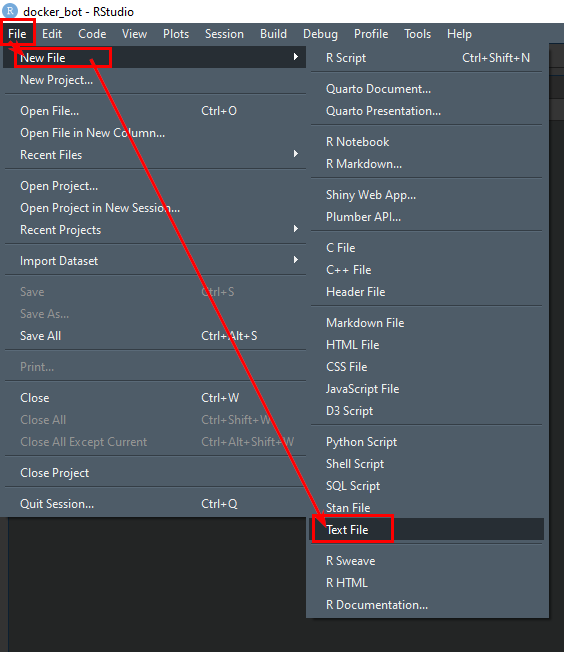
\includegraphics{img/8-4.png}

Докер файл будет содержать следующие команды:

\begin{Shaded}
\begin{Highlighting}[]
\KeywordTok{FROM}\NormalTok{ rocker/r{-}ver:4.2.1}

\KeywordTok{RUN} \FunctionTok{mkdir}\NormalTok{ /home/bot}
\KeywordTok{RUN} \FunctionTok{mkdir}\NormalTok{ /home/bot/log}

\KeywordTok{ENV}\NormalTok{ R\_TELEGRAM\_BOT\_botname ТОКЕН\_ВАШЕГО\_БОТА}

\KeywordTok{COPY}\NormalTok{ bot.R /home/bot/bot.R}

\KeywordTok{RUN} \ExtensionTok{R} \AttributeTok{{-}e} \StringTok{"install.packages(c(\textquotesingle{}telegram.bot\textquotesingle{}, \textquotesingle{}stringr\textquotesingle{}, \textquotesingle{}future\textquotesingle{}, \textquotesingle{}promises\textquotesingle{},\textquotesingle{}fastmap\textquotesingle{}, \textquotesingle{}lgr\textquotesingle{}))"}

\KeywordTok{CMD} \BuiltInTok{cd}\NormalTok{ /home/bot }\DataTypeTok{\textbackslash{}}
  \KeywordTok{\&\&}  \ExtensionTok{R} \AttributeTok{{-}e} \StringTok{"source(\textquotesingle{}/home/bot/bot.R\textquotesingle{})"}
\end{Highlighting}
\end{Shaded}

Тут давайте остановимся и разберём отдельно каждую команду:

\begin{enumerate}
\def\labelenumi{\arabic{enumi}.}
\tightlist
\item
  \texttt{FROM\ rocker/r-ver:4.2.1}, создаёт среду с установленным R 4.2.1, вы можете указать любую, нужную вам версию R.
\item
  \texttt{RUN\ mkdir\ /home/bot} и \texttt{RUN\ mkdir\ /home/bot/log} создаёт в контейнере папку \texttt{bot}, и папку \texttt{log} внутри неё.
\item
  \texttt{ENV\ R\_TELEGRAM\_BOT\_botname\ ТОКЕН\_ВАШЕГО\_БОТА} эта команда создаёт переменную среды \texttt{R\_TELEGRAM\_BOT\_botname} внутри контейнера. В данную переменную передайте токен вашего бота.
\item
  \texttt{COPY\ bot.R\ /home/bot/bot.R} копирует скрипт с кодом нашего бота в контейнер.
\item
  \texttt{RUN\ R\ -e\ "install.packages(c(\textquotesingle{}telegram.bot\textquotesingle{},\ \textquotesingle{}stringr\textquotesingle{},\ \textquotesingle{}future\textquotesingle{},\ \textquotesingle{}promises\textquotesingle{},\textquotesingle{}fastmap\textquotesingle{},\ \textquotesingle{}lgr\textquotesingle{}))"}, конструкция \texttt{RUN\ R\ -e\ "код\ на\ R"} позволяет запускать внутри контейнера R команды. В данном случае мы устанавливаем все, нужные нам пакеты.
\item
  \texttt{CMD\ cd\ /home/bot}, команда, которая переключает рабочую директорию на /home/bot. Команда \texttt{CMD} запускается каждый раз, при запуске контейнера.
\item
  \texttt{\&\&\ R\ -e\ "source(\textquotesingle{}/home/analysis/bot.R\textquotesingle{})"}, объединяется с предыдущей командой, и запускает скрипт бота.
\end{enumerate}

Если вам необходимы определённые версии используемых пакетов то вы можете заменить команду из 5 пункта на:

\begin{Shaded}
\begin{Highlighting}[]
\KeywordTok{RUN} \ExtensionTok{R} \AttributeTok{{-}e} \StringTok{"install.packages(\textquotesingle{}remotes\textquotesingle{}); }\DataTypeTok{\textbackslash{}}
\StringTok{  remotes::install\_version(\textquotesingle{}package\_name\textquotesingle{}, \textquotesingle{}0.1.2\textquotesingle{})"}
\end{Highlighting}
\end{Shaded}

Или установить пакет из снимка MRAN на определённую дату:

\begin{Shaded}
\begin{Highlighting}[]
\KeywordTok{RUN} \ExtensionTok{R} \AttributeTok{{-}e} \StringTok{"options(repos = }\DataTypeTok{\textbackslash{}}
\StringTok{  list(CRAN = \textquotesingle{}http://mran.revolutionanalytics.com/snapshot/2022{-}08{-}01/\textquotesingle{})); }\DataTypeTok{\textbackslash{}}
\StringTok{  install.packages(\textquotesingle{}package\_name\textquotesingle{})"}
\end{Highlighting}
\end{Shaded}

\section{Создание образа}\label{ux441ux43eux437ux434ux430ux43dux438ux435-ux43eux431ux440ux430ux437ux430}

Теперь нам необходимо перейти в терминал, и запустить команду создания образа \texttt{docker\ build}. Данная команда требует от вас передачи нескольких параметров:

\begin{enumerate}
\def\labelenumi{\arabic{enumi}.}
\tightlist
\item
  \texttt{-t} - позволяет задать тег вашего образа;
\item
  вторым параметром является путь к папке с \texttt{Dockerfile}, если вы создали \texttt{Dockerfile} в текущем рабочем каталоге проекта, то просто в качестве этого параметра передайте точку.
\end{enumerate}

Т.е. для создания образа перейдите в терминал (найти терминал можно на соседней вкладке с консолью в RStudio) и запустите в терминале (не в консоли RStudio, а именно в терминале!) следующую команду:

\begin{verbatim}
docker build -t rbot .
\end{verbatim}

\section{Запуск контейнера}\label{ux437ux430ux43fux443ux441ux43a-ux43aux43eux43dux442ux435ux439ux43dux435ux440ux430}

Итак, теперь у нас уже есть собранный Docker образ с нашим ботом, и нам остаётся запустить его командой \texttt{docker\ run}. При запуске контейнера вам необходимо указать следующие параметры:

\begin{enumerate}
\def\labelenumi{\arabic{enumi}.}
\tightlist
\item
  \texttt{-\/-name} позволяет задать название контейнера
\item
  \texttt{-d} флаг, который запускает контейнер в фоновом режиме, не блокируя терминал
\item
  последним параметром мы задаём имя образа, на основе которого будет запущен контейнер.
\end{enumerate}

\begin{verbatim}
docker run --name my_bot -d rbot
\end{verbatim}

Дополнительно мы могли указать флаг \texttt{-\/-rm}, который автоматически удалит контейнер после его остановки.

\begin{verbatim}
docker run --name my_bot -d --rm rbot
\end{verbatim}

\section{Прокидываем токен бота в контейнер при его запуске}\label{ux43fux440ux43eux43aux438ux434ux44bux432ux430ux435ux43c-ux442ux43eux43aux435ux43d-ux431ux43eux442ux430-ux432-ux43aux43eux43dux442ux435ux439ux43dux435ux440-ux43fux440ux438-ux435ux433ux43e-ux437ux430ux43fux443ux441ux43aux435}

В примере выше мы указывали токен нашего бота непосредственно в \texttt{Dockerfile} с помощью команды \texttt{ENV\ R\_TELEGRAM\_BOT\_botname\ ТОКЕН\_ВАШЕГО\_БОТА}. Это не всегда удобно, например, вам может понадобиться возможность указывать токен бота непосредственно при запуске контейнера и вам не хочется постоянно редактировать \texttt{Dockerfile}. В таком случае вы можете прокидывать переменные среды при запуске контейнера используя флаг \texttt{-e}.

Вы можете удалить из \texttt{Dockerfile} команду \texttt{ENV\ R\_TELEGRAM\_BOT\_botname\ ТОКЕН\_ВАШЕГО\_БОТА}, и прокинуть эту же переменную непосредственно при запуске контейнера.

\begin{verbatim}
docker run --name my_bot -d --rm -e R_TELEGRAM_BOT_botname="ТОКЕН_ВАШЕГО_БОТА" rbot
\end{verbatim}

\section{Политика перезапуска бота}\label{ux43fux43eux43bux438ux442ux438ux43aux430-ux43fux435ux440ux435ux437ux430ux43fux443ux441ux43aux430-ux431ux43eux442ux430}

В главе ``\hyperref[ux43fux43eux432ux44bux448ux430ux435ux43c-ux441ux442ux430ux431ux438ux43bux44cux43dux43eux441ux442ux44c-ux440ux430ux431ux43eux442ux44b-ux431ux43eux442ux430]{Повышаем стабильность работы бота}'' мы разобрались, как написать бота, который автоматически перезапускается в случае падения.

При запуске бота через docker контейнер, у вас есть отдельная опция \texttt{-\/-restart}, которая позволяет более гибко управлять перезапуском вашего бота. Данная опция принимает одно из следующих значений:

\begin{itemize}
\tightlist
\item
  \texttt{no} - Не перезапускать контейнер после завершения. Это значение по умолчанию.
\item
  \texttt{on-failure{[}:max-retries{]}} - Перезапускает контейнер если он завершился с не нулевым статусом (т.е. завершился с ошибкой). Опционально можно указать количество попыток перезапуска. Это наиболее подходящая опция для работы бота, т.к. вы можете добавить боту метод остановки пуллинга, и он при запуске команды остановки успешно выключиться, а в случае аварийной остановки - будет перезапущен.
\item
  \texttt{always} - Всегда перезапускает контейнер в не зависимости от статуса завершения. Когда вы выбираете данный вариант, Docker демон будет пытаться перезапустить контейнер бесконечное число раз. Также контейнер будет всегда запускаться при запуске демона, не зависимо от текущего состояния контейнера. В данном случае у вас не будет возможности остановить бота.
\item
  \texttt{unless-stopped} - Всегда перезапускает контейнер не зависимо от статуса завершения, но контейнер не будет запускаться при запуске демона, если контейнер до этого был остановлен вручную.
\end{itemize}

Т.е. следующая команда позволяет запустить бота, который автоматически будет перезапуска в случае ошибки, но при этом, вы в любой момент сможете остановить его любой командой.

\begin{verbatim}
docker run --name my_bot -d --rm -e --restart=on-failure rbot
\end{verbatim}

Давайте протестируем команду \texttt{/crush} и \texttt{/stop}, как я уже писал ранее, первая имитирует ошибку в работе бота, вторая же корректно останавливает его работу.

Из скрина видно, что даже при выполнении команды \texttt{/crush} вызывающую критическую ошибку и падение бота, сам бот автоматически перезапускается, очищает очередь команд, и продолжает работу.

Команда \texttt{/stop} при этом корректно останавливает работу бота.

\section{Просмотр списка запущенных контейнеров}\label{ux43fux440ux43eux441ux43cux43eux442ux440-ux441ux43fux438ux441ux43aux430-ux437ux430ux43fux443ux449ux435ux43dux43dux44bux445-ux43aux43eux43dux442ux435ux439ux43dux435ux440ux43eux432}

Команда \texttt{docker\ ps} позволяет посмотреть список запущенных в данный момент контейнеров.

\begin{verbatim}
docker ps
\end{verbatim}

\section{Остановка контейнера}\label{ux43eux441ux442ux430ux43dux43eux432ux43aux430-ux43aux43eux43dux442ux435ux439ux43dux435ux440ux430}

Для остановки контейнера используйте команду \texttt{docker\ stop}, передав в качестве единственного аргумента либо id, либо название контейнера, который необходимо остановить, в моём случае равнозначными будет две следующее команды:

\begin{verbatim}
docker stop my_bot
\end{verbatim}

\begin{verbatim}
docker stop d06f8cebe987
\end{verbatim}

\section{Удаление контейнера}\label{ux443ux434ux430ux43bux435ux43dux438ux435-ux43aux43eux43dux442ux435ux439ux43dux435ux440ux430}

После остановки контейнера с ботом вы можете его удалить командой \texttt{docker\ rm} передав ей имя контейнера.

\begin{verbatim}
docker rm my_bot
\end{verbatim}

\section{Публикация образа в Docker hub}\label{ux43fux443ux431ux43bux438ux43aux430ux446ux438ux44f-ux43eux431ux440ux430ux437ux430-ux432-docker-hub}

На данном этапе мы уже разобрались с тем, как устроен Docker, и узнали его основные команды. Но пока мы работали с образами, и запускали контейнеры локально, на ПК на котором мы эти образы собирали. Вся мощь Docker заключается в том, что собранные образы очень легко можно переносить на любой другой ПК, единственное требование - наличие на нём установленного Docker.

Для такого переноса удобно использовать \href{https://hub.docker.com/}{docker-hub}, для начала перейдите по ссылке и зарегистрируйтесь там.

Далее возвращаемся в терминал RStudio, логинимся в Docker-hub.

\begin{verbatim}
docker login
\end{verbatim}

Далее введите свой логин и пароль, или ключ API вместо пароля. Теперь нам необходимо добавить нужный тег нашему образу для его публикации. Команда \texttt{tag} принимает два аргумента, имя образа, которому надо присвоить тег, и сам тег. Присваиваемый тег должен иметь следующий вид \texttt{username/repository}, т.е. имя пользователя на Docker-hub и название репозитория, куда вы хотите опубликовать образ.

\begin{verbatim}
docker tag rbot username/rbot
\end{verbatim}

Следующая команда позволяет опубликовать образ на Docker-hub:

\begin{verbatim}
docker push username/rbot
\end{verbatim}

Теперь вы можете загрузить опубликованный ранее образ на любой ПК, независимо от того, какая на нём установлена операционная система, главное предварительно установите на него сам Docker. Используйте следующую команду, что бы забрать образ из Docker-hub:

\begin{verbatim}
docker pull username/rbot
\end{verbatim}

После чего образ будет загружен в ваш локальный реестр образов, убедиться в этом можно с помощью команды \texttt{docker\ images}. Процесс запуска контейнера из загруженного образа ничем не отличается от \hyperref[ux437ux430ux43fux443ux441ux43a-ux43aux43eux43dux442ux435ux439ux43dux435ux440ux430]{описанного выше} в этой главе.

\begin{quote}
Обратите внимание, если вы планируете опубликовать образ с публичным доступом, то не включайте в \texttt{Dockerfile} секретные данные, такие как токен бота или пароли. Рекомендованным способом передачи секретных данных в контейнер является прокинуть необходимые переменные с этими данными непосредственно при запуске контейнера как описано в разделе \hyperref[ux43fux440ux43eux43aux438ux434ux44bux432ux430ux435ux43c-ux442ux43eux43aux435ux43d-ux431ux43eux442ux430-ux432-ux43aux43eux43dux442ux435ux439ux43dux435ux440-ux43fux440ux438-ux435ux433ux43e-ux437ux430ux43fux443ux441ux43aux435]{Прокидываем токен бота в контейнер при его запуске}.
\end{quote}

\section{Как создать общую папку для хранения файлов}\label{ux43aux430ux43a-ux441ux43eux437ux434ux430ux442ux44c-ux43eux431ux449ux443ux44e-ux43fux430ux43fux43aux443-ux434ux43bux44f-ux445ux440ux430ux43dux435ux43dux438ux44f-ux444ux430ux439ux43bux43eux432}

По умолчанию контейнер является полностью изолированным, т.е. все файлы, которые создаются внутри контейнера, удаляются после его запуска, и все данные которые были в эти файлы записаны, также удаляются.

В ходе работы нашего бота пишется лог, сам файл лога \texttt{bot.log} создаётся внутри контейнера в папке \texttt{log}, и за пределами самого контейнера он не доступен. В коде нашего бота за создание лога отвечает следующие команды:

\begin{Shaded}
\begin{Highlighting}[]
\FunctionTok{library}\NormalTok{(lgr)}

\CommentTok{\# Включаем логгер}
\NormalTok{lg }\OtherTok{\textless{}{-}} \FunctionTok{get\_logger}\NormalTok{()}
\NormalTok{lg}\SpecialCharTok{$}\FunctionTok{set\_appenders}\NormalTok{(AppenderFile}\SpecialCharTok{$}\FunctionTok{new}\NormalTok{(}\AttributeTok{file =} \StringTok{\textquotesingle{}log/bot.log\textquotesingle{}}\NormalTok{))}
\NormalTok{lg}\SpecialCharTok{$}\FunctionTok{info}\NormalTok{(}\StringTok{\textquotesingle{}Bot start\textquotesingle{}}\NormalTok{)}
\end{Highlighting}
\end{Shaded}

\begin{quote}
Если вы до этого момента не знакомы с процессом логирования, то рекомендую либо ознакомиться со статьёй ``\href{https://habr.com/ru/post/529118/}{Логирование выполнения скриптов на языке R, пакет lgr}'', либо видео уроком ``\href{https://www.youtube.com/watch?v=xA8YGxQH1Ws}{Логирование процесса выполнения скриптов на языке R (пакеты lgr / lgrExtra)}''.
\end{quote}

В данном случае лог пишется в обычный текстовый файл. Но функционал может быть гораздо шире, чем в рассматриваемом нами примере, бот может работать с базой данных, может принимать какие-то файлы. И нам может потребоваться получить доступ к этим данным.

Для того, что бы организовать на вашем ПК общую с каким либо контейнером папку в Docker есть понятие томов - volume. Но при работе на Windows требуется некоторая предварительная подготовка.

\begin{enumerate}
\def\labelenumi{\arabic{enumi}.}
\tightlist
\item
  Вместе с \texttt{Docker\ toolbox} вы установили несколько программ, включая Oracle VM Virtual Box. Запустите её, если у вас возникает ошибка при запуске VirtualBox, то скорее всего вам необходимо перейти по \href{https://www.virtualbox.org/wiki/Downloads}{ссылке}, и скачать наиболее актуальную версию.
\item
  В Virtual Box выберите дефолтную машину и нажмите ``Настроить'':
\end{enumerate}

\begin{enumerate}
\def\labelenumi{\arabic{enumi}.}
\setcounter{enumi}{2}
\tightlist
\item
  Перейдите в меню ``Общие папки'' и создайте новую общую папку прописав ей путь и дав имя. В моём случае сама папка находится по пути \texttt{D:\textbackslash{}packlab\textbackslash{}docker\_bot\textbackslash{}log}, и имя для неё я задал \texttt{d/packlab/docker\_bot/log}:
\end{enumerate}

\begin{enumerate}
\def\labelenumi{\arabic{enumi}.}
\setcounter{enumi}{3}
\item
  Теперь вернитесь в терминал RStudio и перезапустите виртуальную машину командой \texttt{docker-machine\ restart}.
\item
  После перезагрузки, при запуске контейнера используйте флаг \texttt{-v} и укажите через двоеточие соответствие папки на локальном компьютере с папкой в контейнере. В нашем случае папка на локальном компьютере \texttt{d/packlab/docker\_bot/log} должна быть связана с папкой \texttt{/home/bot/log} в контейнере. Команда будет выглядеть следующим образом:
\end{enumerate}

\begin{verbatim}
docker run --rm --name my_bot -v //d/packlab/docker_bot/log:/home/bot/log rbot
\end{verbatim}

Обратите внимание, я указал двойной слеш \texttt{//} перед именем папки на локальном компьютере, без этого иногда при запуске контейнера возникает ошибка \texttt{invalid\ value\ "C:\textbackslash{}\textbackslash{}..."\ for\ flag\ -v:\ ...:...\ is\ not\ an\ absolute\ path}.

Сразу после запуска у меня в локальной папке \texttt{"D:\textbackslash{}packlab\textbackslash{}docker\_bot\textbackslash{}log"} создаётся файл \texttt{bot.log}, в котором в реальном времени пишется лог работы бота, давайте в этом убедимся:

Содержание локального файла \texttt{bot.log}:

Отставание на 4 часа между временем в telegram, и файлом лога объясняется тем, что в контейнере по умолчанию установлен другой часовой пояс - UTC.

\section{Полезные ссылки}\label{ux43fux43eux43bux435ux437ux43dux44bux435-ux441ux441ux44bux43bux43aux438}

Как я уже писал в начале главы, в интернете полно информации по работе с Docker, тем не менее тут я приведу небольшую подборку ссылок, которые помогут вам получше с ним разобраться:

\begin{itemize}
\tightlist
\item
  \href{https://youtu.be/QF4ZF857m44}{Основы Docker. Большой практический выпуск}
\item
  \href{https://colinfay.me/docker-r-reproducibility/}{An Introduction to Docker for R Users} (англ.)
\item
  \href{https://habr.com/ru/post/358774/}{Docker под Windows для разработки, разбор подводных камней}
\end{itemize}

\section{Заключение}\label{ux437ux430ux43aux43bux44eux447ux435ux43dux438ux435-7}

Теперь мы умеем упаковывать telegram ботов в контейнер, что даёт несколько следующих преимуществ:

\begin{itemize}
\tightlist
\item
  Вы легко можете перенести вашего бота с ноутбука на сервер, или переносить его между серверами, весь процесс займёт пару минут. Никакой предварительной настройки среды для запуска бота теперь не потребуется.
\item
  У вас появляется более гибкая возможность управления политикой перезапуска бота.
\end{itemize}

Основные команды docker и их параметры, которые вам понадобятся в ходе упаковки, запуска, публикации и загрузки бота:

\begin{itemize}
\tightlist
\item
  \texttt{docker\ build} - создать образ:

  \begin{itemize}
  \tightlist
  \item
    \texttt{-t} - тег образа;
  \item
    второй аргумент - путь к папке с \texttt{Dockerfile}.
  \end{itemize}
\item
  \texttt{docker\ run} - запуск контейнера:

  \begin{itemize}
  \tightlist
  \item
    \texttt{-\/-name} - имя контейнера;
  \item
    \texttt{-d} - запускает контейнер в фоновом режиме;
  \item
    \texttt{-\/-rm} - автоматически удаляет контейнер после его остановки;
  \item
    \texttt{-e} - создаёт переменную окружения при запуске контейнера;
  \item
    \texttt{-\/-restart} - управление политикой перезапуска контейнера;
  \item
    \texttt{-v} позволяет прикрепить к контейнеру физическую папку на вашем локальном ПК;
  \item
    последний аргумент - имя образа на основе которого будет запущен контейнер.
  \end{itemize}
\item
  \texttt{docker\ ps} - просмотр списка запущенных контейнеров:

  \begin{itemize}
  \tightlist
  \item
    \texttt{-a} выводит список всех контейнеров, включая остановленные.
  \end{itemize}
\item
  \texttt{docker\ stop} - остановка контейнера:

  \begin{itemize}
  \tightlist
  \item
    в качестве параметра необходимо передать имя или id контейнера.
  \end{itemize}
\item
  \texttt{docker\ rm} - удаление контейнера:

  \begin{itemize}
  \tightlist
  \item
    в качестве параметра необходимо передать имя или id контейнера.
  \end{itemize}
\item
  \texttt{docker\ login} - авторизация в Docker-hub.
\item
  \texttt{docker\ tag} - добавить тег образу:

  \begin{itemize}
  \tightlist
  \item
    локальное название образа, которому надо присвоить тег;
  \item
    название образа в docker-hub по шаблону username/repository.
  \end{itemize}
\item
  \texttt{docker\ push} - опубликовать образ в docker-hub:

  \begin{itemize}
  \tightlist
  \item
    название образа в docker-hub по шаблону username/repository.
  \end{itemize}
\item
  \texttt{docker\ pull} - забрать образ из docker-hub:

  \begin{itemize}
  \tightlist
  \item
    название образа в docker-hub по шаблону username/repository.
  \end{itemize}
\end{itemize}

Отличная работа по упаковке бота в Docker-контейнер! Вы научились использовать Docker для удобного управления и развертывания вашего бота. В последней главе мы развернем бота на Google Cloud Run, чтобы обеспечить его масштабируемость и доступность. Это финальный шаг в нашем путешествии, и вы скоро увидите, как все ваши знания и навыки воплотятся в рабочем облачном решении.

\chapter{Разворачиваем бота в облачных сервисах}\label{ux440ux430ux437ux432ux43eux440ux430ux447ux438ux432ux430ux435ux43c-ux431ux43eux442ux430-ux432-ux43eux431ux43bux430ux447ux43dux44bux445-ux441ux435ux440ux432ux438ux441ux430ux445}

Поздравляю с завершением предыдущих этапов! Мы подходим к финальной части нашего путешествия, и в этой главе мы сосредоточимся на важном шаге --- развертывании вашего бота на Google Cloud Run. Это позволит вашему боту работать в облаке, обеспечивая масштабируемость и надежность.

Важной частью этого процесса является настройка технологии Webhook, которая позволяет вашему боту получать обновления в реальном времени. Мы подробно рассмотрим, как настроить Webhook для вашего бота, чтобы он мог эффективно обрабатывать входящие сообщения и команды от пользователей. Эта технология обеспечивает мгновенную доставку данных и позволяет вашему боту реагировать на события практически моментально.

Мы также изучим, как использовать Google Cloud Run для размещения вашего бота, рассмотрим его настройку и управление окружением. Это обеспечит надежную работу вашего бота и упростит его масштабирование при необходимости.

В завершение главы вы будете готовы запустить своего бота в облаке, и все ваши знания и навыки будут полностью реализованы в рабочем решении.

\begin{quote}
Для того что бы повторить действия описанные в этой главе вам понадобится установить следующее ПО:

\begin{itemize}
\tightlist
\item
  \href{https://www.docker.com/products/docker-desktop/}{Docker Desktop}
\item
  \href{https://git-scm.com/downloads}{Git}
\item
  \href{https://cloud.google.com/sdk/docs/install-sdk}{Google Cloud SDK Shell}
\item
  \href{https://devcenter.heroku.com/articles/heroku-cli\#install-the-heroku-cli}{Heroku CLI}
\end{itemize}
\end{quote}

После установки Docker Desktop перезагрузите ПК,и запуститье эту программу.

\section{Google Cloud Run}\label{google-cloud-run}

\subsection{Условные обозначения}\label{ux443ux441ux43bux43eux432ux43dux44bux435-ux43eux431ux43eux437ux43dux430ux447ux435ux43dux438ux44f}

В этой главе мы много будем работать с командной сторокой, и облачными сервисами. В примерах команд, которые мы будем использовать вы увидите специальные обозначения =, они будут выделены квадратными скобками, и написаны большими буквами. Эти значения необходимо заменить на ваши:

\begin{itemize}
\tightlist
\item
  \texttt{{[}PROJECT\ ID{]}} - Id проекта в Google Cloud
\item
  \texttt{{[}IMAGE\ NAME{]}} - Название Docker образа
\item
  \texttt{{[}CONTAINER\ NAME{]}} - Название Docker контейнера
\item
  \texttt{{[}JOB\ NAME{]}} - Название задания в Google Cloud Run
\item
  \texttt{{[}SCHEDULER\ JOB\ NAME{]}} - Название триггера в Google Cloud Run Job
\item
  \texttt{{[}SERVICE\ NAME{]}} - Название сервиса в Google Cloud Run
\end{itemize}

Т.е. если вы решили назвать Docker образ ``my-bot'', а идентификатор вашего проекта в Google Cloud ``tg-bot-091276''. То следующую команду:

\begin{verbatim}
docker push gcr.io/[PROJECT ID]/[IMAGE NAME]
\end{verbatim}

Необходимо заменить на:

\begin{verbatim}
docker push gcr.io/tg-bot-091276/my-bot
\end{verbatim}

\subsection{Введение в Google Cloude Run}\label{ux432ux432ux435ux434ux435ux43dux438ux435-ux432-google-cloude-run}

Google Cloud Run --- это полностью управляемый сервис от Google Cloud, который позволяет развёртывать и масштабировать контейнерные приложения. Он предназначен для запуска HTTP-приложений и других серверных функций без необходимости управления серверной инфраструктурой. Основные преимущества Cloud Run включают автоматическое масштабирование, оплату только за фактическое использование и интеграцию с другими сервисами Google Cloud.

\subsubsection{Services и Jobs в Google Cloud Run}\label{services-ux438-jobs-ux432-google-cloud-run}

Google Cloud Run позволяет вам создать 2 типа заданий:

\textbf{Jobs (Задачи):}
Cloud Run Jobs предназначены для выполнения одноразовых или периодических задач, которые не требуют HTTP-запросов. Это может быть полезно для различных сценариев, таких как обработка данных, резервное копирование, пакетная обработка и т. д. Ключевые характеристики задач:

\begin{itemize}
\tightlist
\item
  Ограниченное выполнение: Задачи запускаются по требованию и выполняются один раз.
\item
  Асинхронные операции: Задачи могут выполняться в фоновом режиме, не требуя взаимодействия с пользователем.
\item
  Параллельные задания: Возможность запуска множества экземпляров задачи для параллельной обработки данных.
\end{itemize}

Пример использования:

\begin{itemize}
\tightlist
\item
  Ежедневное резервное копирование базы данных.
\item
  Обработка очередей задач из очереди сообщений.
\item
  Конвертация и обработка изображений по расписанию.
\end{itemize}

\textbf{Services (Сервисы)}
Cloud Run Services предназначены для обслуживания HTTP-запросов. Это означает, что они используются для развёртывания веб-приложений, API и других HTTP-сервисов. Вот некоторые ключевые характеристики сервисов:

HTTP-триггеры: Сервисы обрабатывают HTTP-запросы и возвращают HTTP-ответы.
Автоматическое масштабирование: Сервисы автоматически масштабируются в зависимости от нагрузки --- от нуля до бесконечности контейнеров.
Статическое и динамическое содержание: Могут обрабатывать как статические файлы, так и динамически генерируемые данные.
Настройка URL и доменов: Возможность привязки пользовательских доменов и маршрутизации трафика.

Пример использования:

\begin{itemize}
\tightlist
\item
  Telegram боты.
\item
  RESTful API для мобильного приложения.
\item
  Прокси-сервис для обработки и маршрутизации HTTP-запросов
\end{itemize}

То есть, с помощью Job мы можем настроить запуск скрипта по расписанию, например, уже знакомого нам по первой главе скрипта, который запрашивает курсы валют и отправляет их в Telegram. С помощью Service мы можем развернуть полноценного бота с поддержкой команд и клавиатур, который будет обрабатывать запросы пользователей. Далее разберёмся с обеими функциями Google Cloud Run.

\subsection{Как настроить запуск скрипта по рассписанию с помощью Google Cloude Run Job}\label{ux43aux430ux43a-ux43dux430ux441ux442ux440ux43eux438ux442ux44c-ux437ux430ux43fux443ux441ux43a-ux441ux43aux440ux438ux43fux442ux430-ux43fux43e-ux440ux430ux441ux441ux43fux438ux441ux430ux43dux438ux44e-ux441-ux43fux43eux43cux43eux449ux44cux44e-google-cloude-run-job}

\subsubsection{Видео}\label{ux432ux438ux434ux435ux43e}

\subsubsection{Обзор рабочего процесса}\label{ux43eux431ux437ux43eux440-ux440ux430ux431ux43eux447ux435ux433ux43e-ux43fux440ux43eux446ux435ux441ux441ux430-1}

Весь рабочий процесс по настройке запуска R-скрипта по расписанию выглядит следующим образом:

\begin{enumerate}
\def\labelenumi{\arabic{enumi}.}
\tightlist
\item
  Создайте и настройте проект в Google Cloud.
\item
  Напишите R-скрипт, который планируете запускать по расписанию.
\item
  Создайте Dockerfile для создания образа, на основе которого будет создаваться контейнер.
\item
  Проведите тестовую сборку образа и запуск контейнера.
\item
  С помощью Google Cloud SDK инициализируйте командную строку с вашим проектом в Google Cloud.
\item
  Тегируйте и загрузите Docker-образ в Google Container Registry.
\item
  Настройте Job в Google Cloud Run.
\item
  Создайте триггер для запуска созданной Job.
\end{enumerate}

Теперь давайте рассмотрим каждый из этих шагов подробнее.

\subsubsection{Настройка проекта в Google Cloud}\label{ux43dux430ux441ux442ux440ux43eux439ux43aux430-ux43fux440ux43eux435ux43aux442ux430-ux432-google-cloud}

\begin{enumerate}
\def\labelenumi{\arabic{enumi}.}
\tightlist
\item
  Переходим в \href{https://console.cloud.google.com/welcome}{Google Cloud Console}
\item
  С помощью выпадающего меню в верхнем левом углу экрана создаём новый проект
\item
  Переходим в созданный проект
\item
  Включаем в проекте необходимые API сервисы, в левом меню:

  \begin{enumerate}
  \def\labelenumii{\arabic{enumii}.}
  \tightlist
  \item
    Cloud Run Admin API
  \item
    Google Schedule API
  \item
    Artifact Registry API
  \end{enumerate}
\end{enumerate}

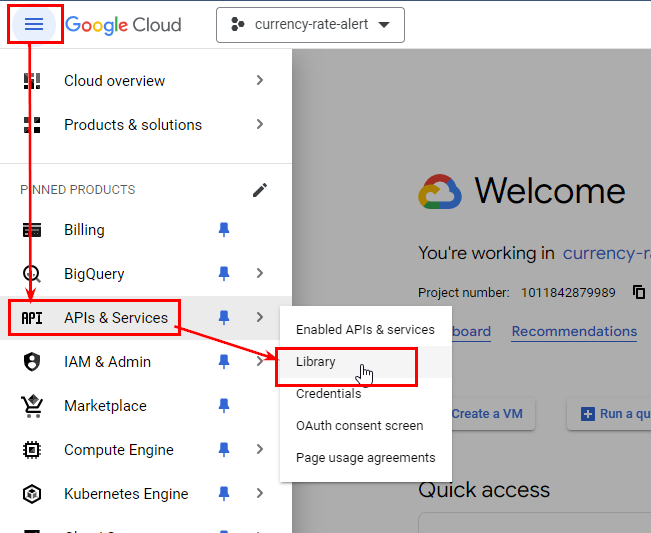
\includegraphics{img/9-1.png}

При желании активировать необходимые API вы сможете позже через Google Cloud SDK.

\subsubsection{Скрипт который будем разворачивать в Google Cloud Run}\label{ux441ux43aux440ux438ux43fux442-ux43aux43eux442ux43eux440ux44bux439-ux431ux443ux434ux435ux43c-ux440ux430ux437ux432ux43eux440ux430ux447ux438ux432ux430ux442ux44c-ux432-google-cloud-run}

Ниже приведен листинг скрипта, который мы будем запускать по расписанию:

\begin{Shaded}
\begin{Highlighting}[]
\FunctionTok{library}\NormalTok{(httr)}
\FunctionTok{library}\NormalTok{(jsonlite)}
\FunctionTok{library}\NormalTok{(telegram.bot)}
\FunctionTok{library}\NormalTok{(stringr)}

\NormalTok{get\_exchange\_rate }\OtherTok{\textless{}{-}} \ControlFlowTok{function}\NormalTok{(api\_key) \{}
\NormalTok{  url }\OtherTok{\textless{}{-}} \FunctionTok{paste0}\NormalTok{(}\StringTok{"https://api.exchangerate{-}api.com/v4/latest/USD?apikey="}\NormalTok{, api\_key)}
\NormalTok{  response }\OtherTok{\textless{}{-}} \FunctionTok{GET}\NormalTok{(url)}
\NormalTok{  data }\OtherTok{\textless{}{-}} \FunctionTok{fromJSON}\NormalTok{(}\FunctionTok{content}\NormalTok{(response, }\StringTok{"text"}\NormalTok{))}
  \FunctionTok{return}\NormalTok{(data)}
\NormalTok{\}}

\NormalTok{send\_telegram\_message }\OtherTok{\textless{}{-}} \ControlFlowTok{function}\NormalTok{(bot\_token, chat\_id, message) \{}
\NormalTok{  bot }\OtherTok{\textless{}{-}} \FunctionTok{Bot}\NormalTok{(}\AttributeTok{token =}\NormalTok{ bot\_token)}
\NormalTok{  bot}\SpecialCharTok{$}\FunctionTok{sendMessage}\NormalTok{(}\AttributeTok{chat\_id =}\NormalTok{ chat\_id, }\AttributeTok{text =}\NormalTok{ message)}
\NormalTok{\}}

\CommentTok{\# Функция для выполнения основного логики}
\NormalTok{execute\_script }\OtherTok{\textless{}{-}} \ControlFlowTok{function}\NormalTok{() \{}
\NormalTok{  api\_key   }\OtherTok{\textless{}{-}} \FunctionTok{Sys.getenv}\NormalTok{(}\StringTok{"EXCHANGE\_RATE\_API\_KEY"}\NormalTok{)}
\NormalTok{  bot\_token }\OtherTok{\textless{}{-}} \FunctionTok{Sys.getenv}\NormalTok{(}\StringTok{"TELEGRAM\_BOT\_TOKEN"}\NormalTok{)}
\NormalTok{  chat\_id   }\OtherTok{\textless{}{-}} \FunctionTok{Sys.getenv}\NormalTok{(}\StringTok{"TELEGRAM\_CHAT\_ID"}\NormalTok{)}
  
\NormalTok{  exchange\_rate }\OtherTok{\textless{}{-}} \FunctionTok{get\_exchange\_rate}\NormalTok{(api\_key)}
\NormalTok{  message }\OtherTok{\textless{}{-}} \FunctionTok{str\_glue}\NormalTok{(}
    \StringTok{"Курс валют на \{Sys.Date()\}"}\NormalTok{,}
    \StringTok{\textquotesingle{}{-}{-}{-}{-}{-}{-}{-}{-}{-}{-}{-}{-}{-}{-}{-}{-}{-}{-}{-}{-}{-}{-}{-}{-}{-}{-}{-}{-}{-}\textquotesingle{}}\NormalTok{,}
    \StringTok{"Курс EUR к USD: \{exchange\_rate$rates$EUR\}"}\NormalTok{, }
    \StringTok{"Курс GBP к USD: \{exchange\_rate$rates$GBP\}"}\NormalTok{,}
    \StringTok{"Курс UAH к USD: \{exchange\_rate$rates$UAH\}"}\NormalTok{,}
    \StringTok{"Курс EGP к USD: \{exchange\_rate$rates$EGP\}"}\NormalTok{, }
    \AttributeTok{.sep =} \StringTok{\textquotesingle{}}\SpecialCharTok{\textbackslash{}n}\StringTok{\textquotesingle{}}
\NormalTok{    )}
  
  \FunctionTok{send\_telegram\_message}\NormalTok{(bot\_token, chat\_id, message)}
\NormalTok{\}}

\CommentTok{\# Выполнение скрипта}
\FunctionTok{execute\_script}\NormalTok{()}
\end{Highlighting}
\end{Shaded}

Чтобы использовать этот же код, вам необходимо получить API-ключ на сайте exchangerate-api.com. Файл с R-кодом в данном случае называется currency\_rates\_alert.R, и это имя файла будет использоваться на следующем шаге.

\subsubsection{Создаём Dockerfile}\label{ux441ux43eux437ux434ux430ux451ux43c-dockerfile}

С Dockerfile и функционалом Docker вы познакомились в предыдущей главе \hyperref[ux443ux43fux430ux43aux43eux432ux44bux432ux430ux435ux43c-ux431ux43eux442ux430-ux432-docker-ux43aux43eux43dux442ux435ux439ux43dux435ux440]{Упаковываем бота в Docker контейнер}. Для нашего скрипта нужен следующий Dockerfile:

\begin{Shaded}
\begin{Highlighting}[]
\KeywordTok{FROM}\NormalTok{ rocker/r{-}base:latest}

\KeywordTok{SHELL}\NormalTok{ [}\StringTok{"/bin/bash"}\NormalTok{, }\StringTok{"{-}o"}\NormalTok{, }\StringTok{"pipefail"}\NormalTok{, }\StringTok{"{-}e"}\NormalTok{, }\StringTok{"{-}u"}\NormalTok{, }\StringTok{"{-}x"}\NormalTok{, }\StringTok{"{-}c"}\NormalTok{]}
\KeywordTok{USER}\NormalTok{ 0}
\KeywordTok{RUN} \ExtensionTok{apt{-}get}\NormalTok{ update }\KeywordTok{\&\&} \ExtensionTok{apt{-}get}\NormalTok{ install }\AttributeTok{{-}y}\NormalTok{ r{-}base r{-}base{-}core r{-}base{-}dev }\DataTypeTok{\textbackslash{}}
\NormalTok{    libcurl4{-}openssl{-}dev libssl{-}dev }\KeywordTok{\&\&} \DataTypeTok{\textbackslash{}}
    \FunctionTok{rm} \AttributeTok{{-}r}\NormalTok{ /var/lib/apt/lists/}\PreprocessorTok{*}

\CommentTok{\# Установка необходимых пакетов}
\KeywordTok{RUN} \ExtensionTok{R} \AttributeTok{{-}e} \StringTok{"install.packages(c(\textquotesingle{}httr\textquotesingle{}, \textquotesingle{}jsonlite\textquotesingle{}, \textquotesingle{}telegram.bot\textquotesingle{}, \textquotesingle{}stringr\textquotesingle{}), repos = \textquotesingle{}http://cran.us.r{-}project.org\textquotesingle{})"}

\CommentTok{\# Копирование R{-}скрипта в контейнер}
\KeywordTok{COPY}\NormalTok{ currency\_rates\_alert.R /app/currency\_rates\_alert.R}

\CommentTok{\# Установка переменных окружения (замените на свои значения)}
\KeywordTok{ENV}\NormalTok{ EXCHANGE\_RATE\_API\_KEY=ВАШ\_API\_КЛЮЧ\_К\_EXCHANGERATE\_API}
\KeywordTok{ENV}\NormalTok{ TELEGRAM\_BOT\_TOKEN=ТОКЕН\_ВАШЕГО\_БОТА}
\KeywordTok{ENV}\NormalTok{ TELEGRAM\_CHAT\_ID=ID\_ЧАТА\_КУДА\_НАДО\_ПРИСЛАТЬ\_СООБЩЕНИЕ}

\CommentTok{\# Запуск R{-}скрипта}
\KeywordTok{CMD}\NormalTok{ [}\StringTok{"Rscript"}\NormalTok{, }\StringTok{"/app/currency\_rates\_alert.R"}\NormalTok{]}
\end{Highlighting}
\end{Shaded}

В Dockerfile замените \texttt{ВАШ\_API\_КЛЮЧ\_К\_EXCHANGERATE\_API}, \texttt{ТОКЕН\_ВАШЕГО\_БОТА} и \texttt{ID\_ЧАТА\_КУДА\_НАДО\_ПРИСЛАТЬ\_СООБЩЕНИЕ} на ваши значения. Так же если файл с вашим R скриптом имеет другое название, то и в Dockerfile его необходимо изменить с \texttt{currency\_rates\_alert.R}.

\subsubsection{Тестовая сборка образа и запуск контейнера}\label{ux442ux435ux441ux442ux43eux432ux430ux44f-ux441ux431ux43eux440ux43aux430-ux43eux431ux440ux430ux437ux430-ux438-ux437ux430ux43fux443ux441ux43a-ux43aux43eux43dux442ux435ux439ux43dux435ux440ux430}

Когда ваш скрипт готов и вы убедились, что он работает, запустив его предварительно в интерактивном режиме RStudio, протестируйте сборку образа и запуск контейнера локально.

давайте перейдём в директорию с нашим проектом, т.е. в папку, в которой у вас хранится R скрипт и Dockerfile:

\begin{verbatim}
cd C:\Users\SAMSUNG\Documents\currency_rates_alert
\end{verbatim}

Замените путь на ваш.

Далее выполним сборку образа и запуск контейнера, для этого следующие команды:

\begin{verbatim}
docker build -t [IMAGE NAME] .
docker run --name [CONTAINER NAME] --rm [IMAGE NAME]
\end{verbatim}

Если контейнер был успешно собран и ваш скрипт выполнился, можно переходить к следующему шагу.

\begin{quote}
Подробности работы с Docker смотрите в главе \hyperref[ux443ux43fux430ux43aux43eux432ux44bux432ux430ux435ux43c-ux431ux43eux442ux430-ux432-docker-ux43aux43eux43dux442ux435ux439ux43dux435ux440]{Упаковываем бота в Docker контейнер}.
\end{quote}

\subsubsection{Инициализация Google Cloud SDK}\label{ux438ux43dux438ux446ux438ux430ux43bux438ux437ux430ux446ux438ux44f-google-cloud-sdk}

Если у вас еще не установлен Google Cloud SDK, следуйте \href{https://cloud.google.com/sdk/docs/install-sdk}{этой инструкции} для его установки. После установки запустите Google Cloud SDK и выполните инициализацию:

\begin{verbatim}
gcloud init
\end{verbatim}

Эта команда откроет веб-браузер, чтобы вы могли войти в Google Cloud и выбрать проект, который будете использовать. После завершения инициализации сохраните конфигурацию.

Далее вам необходимо настроить Docker для работы с Google Container Registry:, воспользуйтесь для этого следующей командой:

\begin{verbatim}
gcloud auth configure-docker
\end{verbatim}

Если при создании проекта вы не активировали нужные API, то на этом шаге вы можете сделать это из командной строки:

\begin{verbatim}
gcloud services enable run.googleapis.com
gcloud services enable cloudscheduler.googleapis.com
gcloud services enable artifactregistry.googleapis.com
\end{verbatim}

Проверить список активированных в проекте API можно следующей командой:

\begin{verbatim}
gcloud services list --enabled
\end{verbatim}

\subsubsection{Тегирование и загрузка Docker-образа в Google Container Registry}\label{ux442ux435ux433ux438ux440ux43eux432ux430ux43dux438ux435-ux438-ux437ux430ux433ux440ux443ux437ux43aux430-docker-ux43eux431ux440ux430ux437ux430-ux432-google-container-registry}

После успешного локального тестирования можно приступать к отравке образа и разворачиванию контейнера в Google Cloud. Но до этого образ необходимо тегорировать. Тегирование Docker-образа необходимо для его идентификации и управления версиями. В контексте работы с Google Container Registry (GCR) тегирование помогает определить, какой именно образ вы хотите загрузить, развернуть или использовать в дальнейшем.

\begin{verbatim}
docker tag [IMAGE NAME] gcr.io/[PROJECT ID]/[IMAGE NAME]
docker push gcr.io/[PROJECT ID]/[IMAGE NAME]
\end{verbatim}

\begin{quote}
Замените {[}PROJECT ID{]} на идентификатор вашего проекта в Google Cloud.
\end{quote}

\subsubsection{Настраиваем Job в Google Cloud Run}\label{ux43dux430ux441ux442ux440ux430ux438ux432ux430ux435ux43c-job-ux432-google-cloud-run}

Для удобства дальнейшей работы перейдите в веб интерфейс сервиса \href{https://console.cloud.google.com/run/jobs}{Google Cloud Run} на вкладку Jobs и нажмите кнопку ``Create Job''.

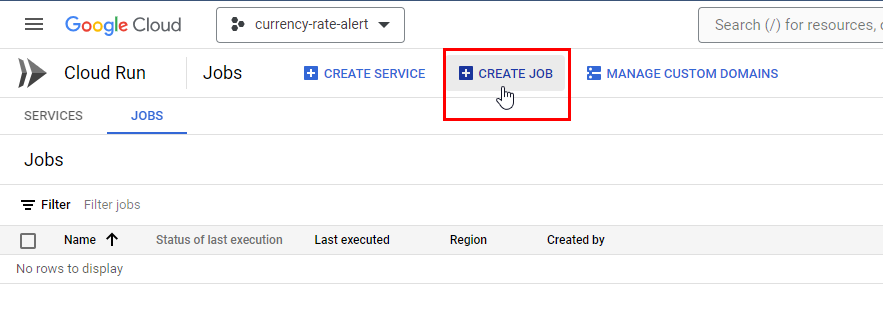
\includegraphics{img/9-3.png}

В поле ``\,'' нажмите кнопку ``Select'' и укажиет загруженный на прошлом шаге образ.

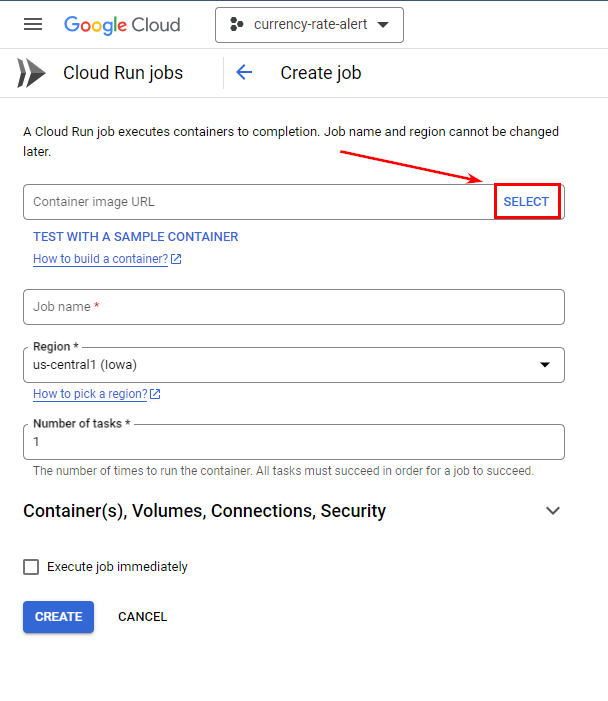
\includegraphics{img/9-4.png}
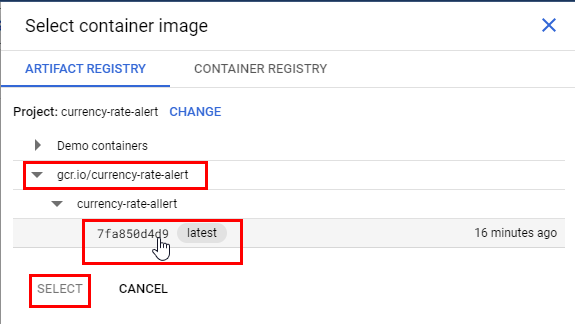
\includegraphics{img/9-5.png}

После чего можете задать произвольное имя для джобы, и нажать ``Create''.

\subsubsection{Тестирование созданной Job в Google Cloud Run}\label{ux442ux435ux441ux442ux438ux440ux43eux432ux430ux43dux438ux435-ux441ux43eux437ux434ux430ux43dux43dux43eux439-job-ux432-google-cloud-run}

Для тестирования просто откройте нужную Job и нажмите ``Execute''. Если задание успешно выполнися то можно переходить на вкладку TRIGGERS и создать расписание запуска.

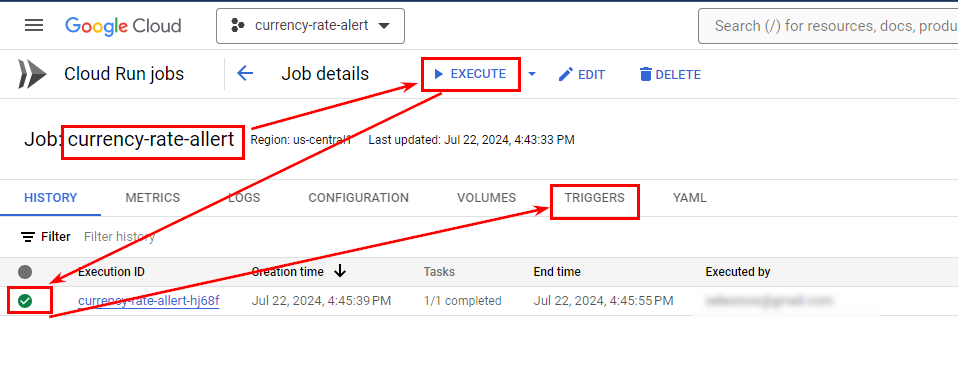
\includegraphics{img/9-6.png}

\subsubsection{Создаём тригер для запуска созданной Job}\label{ux441ux43eux437ux434ux430ux451ux43c-ux442ux440ux438ux433ux435ux440-ux434ux43bux44f-ux437ux430ux43fux443ux441ux43aux430-ux441ux43eux437ux434ux430ux43dux43dux43eux439-job}

Мы на финальном шаге, всё, что нам остаётся это создать триггер для запуска созданного задания. На вкладке ``TRIGGERS'' жмём кнопку ``ADD SCHEDULER TRRIGER''.

В открывшемся диалоговом окне,в поле ``Frequency'' вам необходимо написать CRON выражение, для создания расписания запуска задания. В первой главе мы уже сталкивались с CRON выражении в разделе \hyperref[ux43dux430ux441ux442ux440ux430ux438ux432ux430ux435ux43c-ux437ux430ux43fux443ux441ux43a-ux440ux430ux441ux43fux438ux441ux430ux43dux438ux44f-ux43eux442ux43fux440ux430ux432ux43aux438-ux441ux43eux43eux431ux449ux435ux43dux438ux44f-ux441-ux43fux43eux43cux43eux449ux44cux44e-github-actions]{Настраиваем запуск расписания отправки сообщения с помощью GitHub Actions}. Но я продублирую тут эту информацию.

CRON выражение состоит из 5 значений, любое из которых можно пропустить поставив \texttt{*}:

\begin{itemize}
\tightlist
\item
  Минуты (0-59)
\item
  Часы (0-23)
\item
  День месяца (1-31)
\item
  Месяц (1-12)
\item
  День недели (0-6, где 0 --- воскресенье)
\end{itemize}

Т.е. если мы хотим настроить запуск нашего задание в 10:15 утра каждый понедельник то CRON выражение будет \texttt{15\ 10\ *\ *\ 1}, т.е.:

\begin{itemize}
\tightlist
\item
  15 - это 15 минут
\item
  10 - это 10 часов
\item
  Далее две звезды значит что мы пропускаем месяца и день месяца, они не будут учитываться в расписании.
\item
  1 - понедельник.
\end{itemize}

Но я сейчас создам триггер для запуска скрипта в 10:15 на ежедневной основе, т.е. \texttt{15\ 10\ *\ *\ *}.

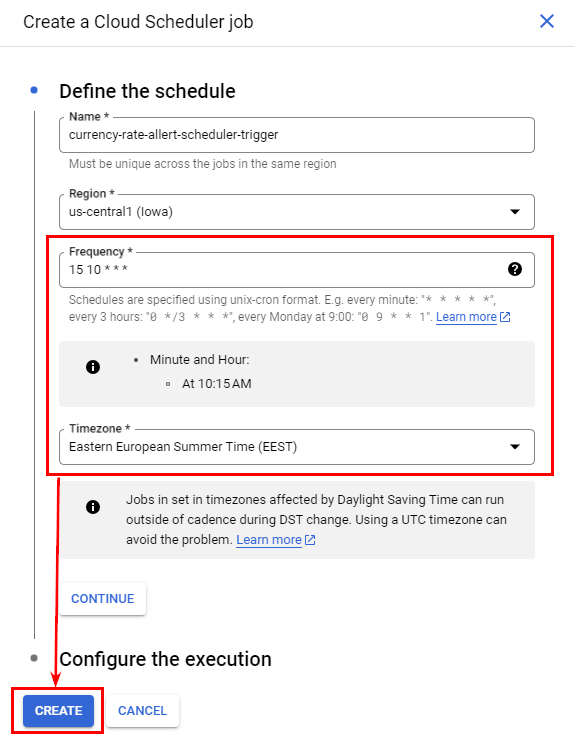
\includegraphics{img/9-7.png}

Так же вы можете нажать ``Continue'' вы можете настроить запуск задания от имени созданного вами сервисного аккаунта, но учтите что в таком случае вам необходимо для этого сервисного аккаунта в разделе IM выдать следующие разрешения:

\begin{enumerate}
\def\labelenumi{\arabic{enumi}.}
\tightlist
\item
  Откройте Google Cloud Console
\item
  Перейдите в раздел ``IAM \& Admin'' \textgreater{} ``IAM''
\item
  Найдите ваш сервисный аккаунт (\href{mailto:service-account-name@ptoj}{\nolinkurl{service-account-name@ptoj}}\_id.iam.gserviceaccount.com)
\item
  Нажмите на карандаш рядом с ним для редактирования разрешений
\item
  Добавьте следующие роли:
\end{enumerate}

\begin{itemize}
\tightlist
\item
  Cloud Run Invoker (roles/run.invoker): Эта роль позволяет сервисному аккаунту запускать Job.
\item
  Cloud Run Developer (roles/run.developer): Эта роль дает возможность создавать, обновлять и удалять Job, а также просматривать их логи.
\item
  Service Account User (roles/iam.serviceAccountUser): Эта роль нужна, если ваш Job выполняется от имени другого сервисного аккаунта.
\end{itemize}

Но, на самом деле создать Job и добавить в неё триггер можно непосредственно из самой консоли:

Создание Job:

\begin{verbatim}
gcloud run jobs create [JOB NAME] --image gcr.io/[PROJECT ID]/[IMAGE NAME] --platform managed
\end{verbatim}

Добавление триггера:

\begin{verbatim}
gcloud scheduler jobs create http [SCHEDULER JOB NAME] \
    --schedule "30 10 * * *" \
    --http-method POST \
    --uri https://YOUR_REGION-run.googleapis.com/v2/projects/YOUR_PROJECT_ID/locations/YOUR_REGION/jobs/YOUR_JOB_NAME:run \
    --oauth-service-account-email YOUR_SERVICE_ACCOUNT_EMAIL \
    --region YOUR_REGION
\end{verbatim}

Но, как по мне проще создавать Job и добавить ей триггеры через Веб интерфейс.

\subsection{Разворачиваем Telegram бота в Google Cloud Run Service}\label{ux440ux430ux437ux432ux43eux440ux430ux447ux438ux432ux430ux435ux43c-telegram-ux431ux43eux442ux430-ux432-google-cloud-run-service}

Как я уже писал в начале этой главе в сервисе Google Cloud Run есть 2 типа заданий, разовое - Job, и постоянное фоновое - Service. Для того, что бы запустить бота, который будет крутится в фоновом режиме и обрабатывать входящие запросы нам необходимо использовать именно Service.

\subsubsection{Видео}\label{ux432ux438ux434ux435ux43e-1}

\subsubsection{Рабочий процесс}\label{ux440ux430ux431ux43eux447ux438ux439-ux43fux440ux43eux446ux435ux441ux441}

При развёртывании бота в Google Cloud Run Service алгоритм ваших действий будет следующим:

\begin{enumerate}
\def\labelenumi{\arabic{enumi}.}
\tightlist
\item
  Напишите скрипт бота, которого планируете развернуть.
\item
  Создайте Dockerfile для создания образа, на основе которого будет создаваться контейнер.
\item
  Проведите тестовую сборку образа и запуск контейнера.
\item
  Создайте и настройте проект в Google Cloud.
\item
  С помощью Google Cloud SDK инициализируйте командную строку с вашим проектом в Google Cloud.
\item
  Тегируйте и загрузите Docker-образ в Google Artifact Registry.
\item
  Запустите бота в Google Cloud Run для того что бы получить Webhook URL.
\item
  Исправьте в переменных среды Webhook URL, выполните повторную сборку, отправку и развёртку вашего бота в Google Cloud Run.
\end{enumerate}

\subsubsection{Webhook вместо polling}\label{webhook-ux432ux43cux435ux441ux442ux43e-polling}

Прилшло время более подробно разобраться с тем, как устроен механизм получения ботом обновлений, и совсем немного окунутся в историю развития клиент серверных технологий.

\paragraph{Разница между механизмами polling и webhook}\label{ux440ux430ux437ux43dux438ux446ux430-ux43cux435ux436ux434ux443-ux43cux435ux445ux430ux43dux438ux437ux43cux430ux43cux438-polling-ux438-webhook}

В ранние годы веб-технологий, когда серверные технологии и базы данных только начинали развиваться, коммуникация между клиентом (в нашем случае машиной на которой работает скрипт вашего бота) и сервером (в нашем случае сервер Telegram API) была довольно простой. Клиенты периодически отправляли запросы к серверу для проверки наличия новых данных. Такой механизм получил название polling.

Polling --- это метод, при котором бот регулярно (с определённым интервалом) отправляет запросы к серверу Telegram для проверки наличия новых обновлений. Внутри класса Updater технически это реализуется так:

\begin{enumerate}
\def\labelenumi{\arabic{enumi}.}
\tightlist
\item
  Бот делает запросы к Telegram API с помощью метода \texttt{getUpdates}.
\item
  Если есть новые сообщения или обновления, сервер Telegram отправляет их боту.
\item
  Бот обрабатывает эти обновления и отвечает на них.
\end{enumerate}

До этого момента во всех примерах, которые я приводил в этой книге мы с вами использовали именно этот механиз получения обновлений. Делали мы это только потому, что его максимально просто запустить на локальной машине. Polling будет работать даже если к машине на которой вы развернули бота нет доступа из внешних ресурсов, firewall блокирует любые попытки достучатся до вашего ПК извне так как нет необходимости в открытых портах для входящих соединений, и даже если у вас динамический IP адрес.

Polling был простым и понятным методом, но с увеличением количества пользователей и данных его эффективность стала проблемой. На смену polling пришел Webhook, который был разработан для решения проблем, связанных с эффективностью и нагрузкой при использовании polling. Webhook представляет собой более современный подход к получению обновлений и был внедрён для улучшения производительности и уменьшения задержек. Работает он по следующей схеме:

\begin{enumerate}
\def\labelenumi{\arabic{enumi}.}
\tightlist
\item
  Бот регистрирует URL для webhook с помощью метода \texttt{setWebhook}.
\item
  Когда есть новое обновление, Telegram отправляет запрос на указанный URL.
\item
  Бот получает и обрабатывает обновление в реальном времени.
\end{enumerate}

Схематично сравнить эти два механизма можно следующим образом:

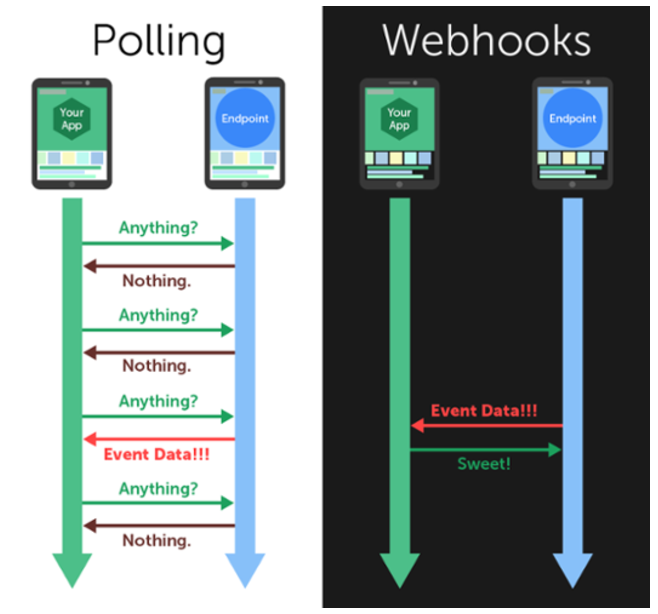
\includegraphics{img/10-pooling-webhook-infographics.png}

Если провести аналогию из реального мира, то представьте, что у вас есть старый почтовый ящик, и каждый день вы отправляетесь к нему, чтобы проверить, пришла ли новая почта. Вы открываете ящик и смотрите, есть ли что-то новое. Если нет, вы возвращаетесь домой и снова идёте проверять на следующий день. Это и есть polling. Теперь представьте, что у вас есть специальный почтальон, который приходит к вам домой каждый раз, когда приходит новая почта. Вместо того, чтобы самому ходить к почтовому ящику, почтальон вам сам звонит в дверь и приносит письмо прямо к вам. Это и есть webhook.

Так вот, запустить механизм polling легко и просто на локальной машине, т.к. от вас не требуется практически никаких дополнительных настроект, но вот облачные технологии стремятся к тому, что бы экономить выделенные ресурсы, поэтому они позволяют вам развернуть бота используя технологию Webhook, Google Cloud Run не является тут исключением. К тому же технология Webhook позволит вам экономить на использовании раздичных облачных систем для развёртования бота, т.к. зачастую вы там платите только за используемые ресурсы.

\paragraph{Реализация webhook в пакете telegram.bot}\label{ux440ux435ux430ux43bux438ux437ux430ux446ux438ux44f-webhook-ux432-ux43fux430ux43aux435ux442ux435-telegram.bot}

Изначально пакет \texttt{telegram.bot} включал в свой функционал только polling, метод обновления данных webhook в него был добавлен только в версии 3.0.0 сторонним разработчиком, но сделано это было по моей просьбе, кому интересно история добавления этого метода началась в этой \href{https://github.com/virtualstaticvoid/heroku-buildpack-r/issues/162}{ветке} на GitHub, а {[}тут{]}9https://github.com/ebeneditos/telegram.bot/pull/27) уже был добавлен класс \texttt{Webhook} в пакет.

Класс \texttt{Webhook} очень похож на \texttt{Updater}, ниже пример работы с ним:

\begin{Shaded}
\begin{Highlighting}[]
\CommentTok{\# Создаём метод start}
\NormalTok{start }\OtherTok{\textless{}{-}} \ControlFlowTok{function}\NormalTok{(bot, update) \{}
\NormalTok{ bot}\SpecialCharTok{$}\FunctionTok{sendMessage}\NormalTok{(}
   \AttributeTok{chat\_id =}\NormalTok{ update}\SpecialCharTok{$}\NormalTok{message}\SpecialCharTok{$}\NormalTok{chat\_id,}
   \AttributeTok{text =} \FunctionTok{sprintf}\NormalTok{(}
     \StringTok{"Hello \%s!"}\NormalTok{,}
\NormalTok{     update}\SpecialCharTok{$}\NormalTok{message}\SpecialCharTok{$}\NormalTok{from}\SpecialCharTok{$}\NormalTok{first\_name}
\NormalTok{   )}
\NormalTok{ )}
\NormalTok{\}}

\CommentTok{\# Инициализируем экземпляр класса Webhook}
\NormalTok{webhook }\OtherTok{\textless{}{-}} \FunctionTok{Webhook}\NormalTok{(}
  \AttributeTok{webhook\_url =} \StringTok{"https://example.com/webhook"}\NormalTok{, }
  \AttributeTok{token       =} \FunctionTok{Sys.getenv}\NormalTok{(}\StringTok{"TOKEN"}\NormalTok{), }
  \AttributeTok{verbose     =} \ConstantTok{TRUE}
\NormalTok{)}

\CommentTok{\# wire up handler}
\NormalTok{webhook }\OtherTok{\textless{}{-}}\NormalTok{ webhook }\SpecialCharTok{+} \FunctionTok{CommandHandler}\NormalTok{(}\StringTok{"start"}\NormalTok{, start)}

\CommentTok{\# start polling}
\NormalTok{webhook}\SpecialCharTok{$}\FunctionTok{start\_server}\NormalTok{(}\AttributeTok{host =} \StringTok{"0.0.0.0"}\NormalTok{, }\AttributeTok{port =} \DecValTok{8080}\NormalTok{)}

\CommentTok{\# stop polling}
\NormalTok{webhook}\SpecialCharTok{$}\FunctionTok{stop\_server}\NormalTok{()}
\end{Highlighting}
\end{Shaded}

Т.е. процесс такой же как и при создании \texttt{Updater}, но помимо токена бота вам ещё необходимо указать webhook url, на который telegram будет присылать для бота обновления. О том как его получить мы поговорим немного позже. Далее, так же как и с Updater, вы просто добавляете в Webhook все обработчики, и запускаете процесс обработки обновления методом \texttt{start\_server()}, который является аналогом \texttt{start\_polling()}.

\subsubsection{Код бота запрашивающего курсы валют}\label{ux43aux43eux434-ux431ux43eux442ux430-ux437ux430ux43fux440ux430ux448ux438ux432ux430ux44eux449ux435ux433ux43e-ux43aux443ux440ux441ux44b-ux432ux430ux43bux44eux442}

В этом разделе мы продолжим развивать тему прошлого раздела о получении информации курсов валют, но теперь мы напишем полноценного бота, которого в любой момент можно спросить курс любой валюты.

Код нашего бота:

\begin{Shaded}
\begin{Highlighting}[]
\FunctionTok{library}\NormalTok{(telegram.bot)}
\FunctionTok{library}\NormalTok{(httr)}
\FunctionTok{library}\NormalTok{(jsonlite)}

\CommentTok{\# Метод запроса курса валют}
\NormalTok{get\_cur\_rate }\OtherTok{\textless{}{-}} \ControlFlowTok{function}\NormalTok{(bot, update, args) \{}
  
\NormalTok{  currency\_code }\OtherTok{\textless{}{-}} \FunctionTok{toupper}\NormalTok{(args)}
\NormalTok{  api\_key }\OtherTok{\textless{}{-}} \FunctionTok{Sys.getenv}\NormalTok{(}\StringTok{\textquotesingle{}EXCHANGERATE\_API\_KEY\textquotesingle{}}\NormalTok{)}
\NormalTok{  url     }\OtherTok{\textless{}{-}} \FunctionTok{paste0}\NormalTok{(}\StringTok{"https://api.exchangerate{-}api.com/v4/latest/USD?apikey="}\NormalTok{, api\_key)}
  
\NormalTok{  response }\OtherTok{\textless{}{-}} \FunctionTok{GET}\NormalTok{(url)}
\NormalTok{  data }\OtherTok{\textless{}{-}} \FunctionTok{fromJSON}\NormalTok{(}\FunctionTok{content}\NormalTok{(response, }\StringTok{"text"}\NormalTok{))}
  
  \ControlFlowTok{if}\NormalTok{ (}\SpecialCharTok{!}\NormalTok{currency\_code }\SpecialCharTok{\%in\%} \FunctionTok{names}\NormalTok{(data}\SpecialCharTok{$}\NormalTok{rates)) \{}
\NormalTok{    bot}\SpecialCharTok{$}\FunctionTok{sendMessage}\NormalTok{(}\AttributeTok{chat\_id =}\NormalTok{ update}\SpecialCharTok{$}\NormalTok{message}\SpecialCharTok{$}\NormalTok{chat\_id, }\AttributeTok{text =} \FunctionTok{paste0}\NormalTok{(args, }\StringTok{" is Invalid currency code."}\NormalTok{))}
    \FunctionTok{return}\NormalTok{(}\ConstantTok{NULL}\NormalTok{)}
\NormalTok{  \}}
  
\NormalTok{  rate }\OtherTok{\textless{}{-}}\NormalTok{ data}\SpecialCharTok{$}\NormalTok{rates[[currency\_code]]}
\NormalTok{  message }\OtherTok{\textless{}{-}} \FunctionTok{sprintf}\NormalTok{(}\StringTok{"Курс \%s к USD: \%f"}\NormalTok{, currency\_code, rate)}
\NormalTok{  bot}\SpecialCharTok{$}\FunctionTok{sendMessage}\NormalTok{(}\AttributeTok{chat\_id =}\NormalTok{ update}\SpecialCharTok{$}\NormalTok{message}\SpecialCharTok{$}\NormalTok{chat\_id, }\AttributeTok{text =}\NormalTok{ message)}
  
\NormalTok{\}}

\CommentTok{\# Создаём Webhook}
\NormalTok{webhook }\OtherTok{\textless{}{-}} \FunctionTok{Webhook}\NormalTok{(}
  \AttributeTok{webhook\_url =} \FunctionTok{Sys.getenv}\NormalTok{(}\StringTok{\textquotesingle{}WEBHOOK\_URL\textquotesingle{}}\NormalTok{), }
  \AttributeTok{token       =} \FunctionTok{bot\_token}\NormalTok{(}\StringTok{\textquotesingle{}CURBOT\textquotesingle{}}\NormalTok{), }
  \AttributeTok{verbose     =} \ConstantTok{TRUE}
\NormalTok{  )}

\CommentTok{\# Добавляем обработчики}
\NormalTok{webhook }\OtherTok{\textless{}{-}}\NormalTok{ webhook }\SpecialCharTok{+} \FunctionTok{CommandHandler}\NormalTok{(}\StringTok{"get\_cur\_rate"}\NormalTok{, get\_cur\_rate, }\AttributeTok{pass\_args =}\NormalTok{ T)}

\CommentTok{\# Запускаем Webhook}
\NormalTok{webhook}\SpecialCharTok{$}\FunctionTok{start\_server}\NormalTok{(}
  \AttributeTok{host =} \StringTok{"0.0.0.0"}\NormalTok{,}
  \AttributeTok{port =} \DecValTok{8080}
\NormalTok{)}
\end{Highlighting}
\end{Shaded}

В основе метода \texttt{get\_cur\_rate} лежит логика, описанная в прошлом разделе. Бот получает сообщение в котором указан код валют, далее запрашивает курсы из exchangerate-api, парсит результат, и отправляет в ответе курс по указанной ранее валюте.

Далее мы инициализируем объект класса Webhook, и передаём в аргумент \texttt{webhook\_url} значение переменной среды \texttt{WEBHOOK\_URL}, а в аргумент \texttt{token}, значение переменной \texttt{R\_TELEGRAM\_BOT\_CURBOT}. Значения этих переменных мы будем задавать в Dockerfile.

\subsubsection{Собираем Docker образ}\label{ux441ux43eux431ux438ux440ux430ux435ux43c-docker-ux43eux431ux440ux430ux437}

Для сборки нужного Docker образа мы прописываем следующий Dockerfile:

\begin{Shaded}
\begin{Highlighting}[]
\CommentTok{\# Use the official R base image}
\KeywordTok{FROM}\NormalTok{ rocker/r{-}ver:4.1.0}

\CommentTok{\# Set the shell}
\KeywordTok{SHELL}\NormalTok{ [}\StringTok{"/bin/bash"}\NormalTok{, }\StringTok{"{-}o"}\NormalTok{, }\StringTok{"pipefail"}\NormalTok{, }\StringTok{"{-}e"}\NormalTok{, }\StringTok{"{-}u"}\NormalTok{, }\StringTok{"{-}x"}\NormalTok{, }\StringTok{"{-}c"}\NormalTok{]}

\CommentTok{\# Install necessary system dependencies}
\KeywordTok{USER}\NormalTok{ root}
\KeywordTok{RUN} \ExtensionTok{apt{-}get}\NormalTok{ update }\KeywordTok{\&\&} \ExtensionTok{apt{-}get}\NormalTok{ install }\AttributeTok{{-}y} \DataTypeTok{\textbackslash{}}
\NormalTok{    libcurl4{-}openssl{-}dev }\DataTypeTok{\textbackslash{}}
\NormalTok{    libssl{-}dev }\DataTypeTok{\textbackslash{}}
    \KeywordTok{\&\&} \FunctionTok{rm} \AttributeTok{{-}rf}\NormalTok{ /var/lib/apt/lists/}\PreprocessorTok{*}

\CommentTok{\# Install necessary R packages}
\KeywordTok{RUN} \ExtensionTok{R} \AttributeTok{{-}e} \StringTok{"install.packages(c(\textquotesingle{}httr\textquotesingle{}, \textquotesingle{}jsonlite\textquotesingle{}))"}
\KeywordTok{RUN} \ExtensionTok{R} \AttributeTok{{-}e} \StringTok{"install.packages(\textquotesingle{}telegram.bot\textquotesingle{}, repos = \textquotesingle{}http://cran.us.r{-}project.org\textquotesingle{})"}

\KeywordTok{ENV}\NormalTok{ EXCHANGERATE\_API\_KEY=[ВАШ КЛЮЧ В exchangerate{-}api.com]}
\KeywordTok{ENV}\NormalTok{ R\_TELEGRAM\_BOT\_CURBOT=[ТОКЕН ВАШЕГО БОТА]}
\KeywordTok{ENV}\NormalTok{ WEBHOOK\_URL=https://my{-}service.a.run.app/webhook}

\CommentTok{\# Copy the R script to the container}
\KeywordTok{COPY}\NormalTok{ curbot.R /app/curbot.R}

\CommentTok{\# Set the working directory}
\KeywordTok{WORKDIR}\NormalTok{ /app}

\CommentTok{\# Run the R script}
\KeywordTok{CMD}\NormalTok{ [}\StringTok{"Rscript"}\NormalTok{, }\StringTok{"/app/curbot.R"}\NormalTok{]}
\end{Highlighting}
\end{Shaded}

На данном этапе этапе мы ещё не знаем URL нашего сервиса, поэтому в переменную WEBHOOK\_URL пока что прописываем совершенно любой URL, можно даже не работающий. На второй итерации развёртки мы будем заменять значение этой переменной.

Далее выполним локальную сборку образа, и тестовый локальный запуск контейнера.

\begin{verbatim}
docker build -t [IMAGE NAME] .
docker run --name [CONTAINER NAME] --rm [IMAGE NAME]
\end{verbatim}

Если контейнер был успешно запущен на этом этапе в консоли вы увидите примерно такое сообщение:

\begin{verbatim}
Starting webhook server...
Listening on '0.0.0.0:8080'...
Configuring webhook 'https://currency-bot-xxxxxxxx-ew.a.run.app'...
Waiting for requests...
\end{verbatim}

Это говорит о том, что контейнер был успешно запущен. Теперь перейдите в Docker и остановите этот контейнер, ваш бот на этом этапе отвечать на запросы не будет.

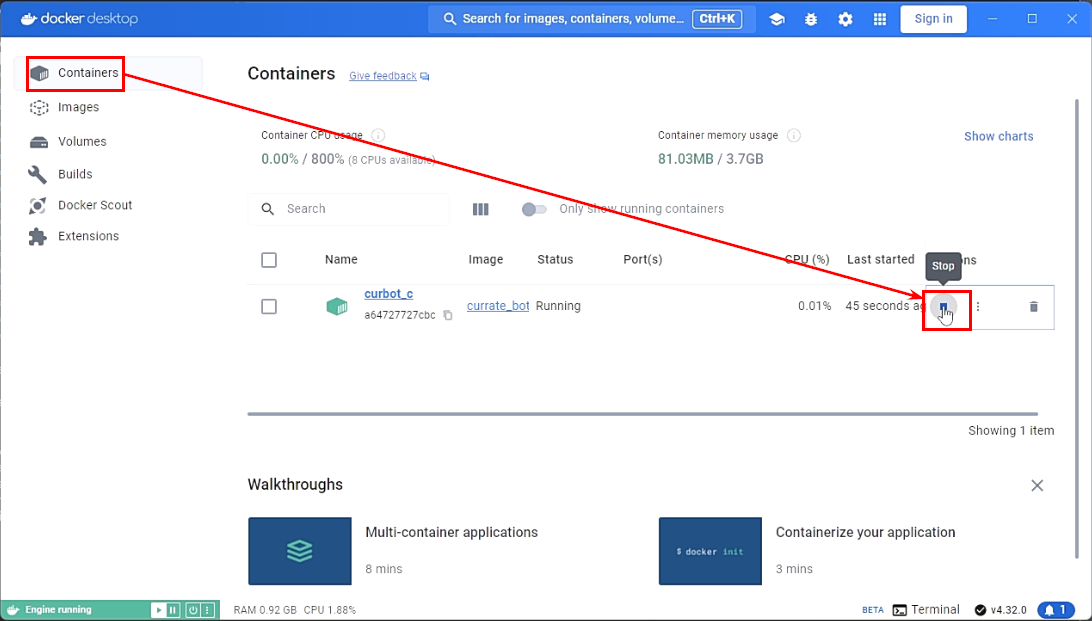
\includegraphics{img/9-8.png}

\subsubsection{Создание и настройка проекта в Google Cloud}\label{ux441ux43eux437ux434ux430ux43dux438ux435-ux438-ux43dux430ux441ux442ux440ux43eux439ux43aux430-ux43fux440ux43eux435ux43aux442ux430-ux432-google-cloud}

\begin{enumerate}
\def\labelenumi{\arabic{enumi}.}
\tightlist
\item
  Переходим в \href{https://console.cloud.google.com/welcome}{Google Cloud Console}
\item
  С помощью выпадающего меню в верхнем левом углу экрана создаём новый проект
\item
  Переходим в созданный проект
\item
  Включаем в проекте необходимые API сервисы, в левом меню:

  \begin{enumerate}
  \def\labelenumii{\arabic{enumii}.}
  \tightlist
  \item
    Cloud Run Admin API
  \item
    Artifact Registry API
  \end{enumerate}
\end{enumerate}

Включить данные API можно будет и с помощью Google Cloud SDK на следующем шаге.

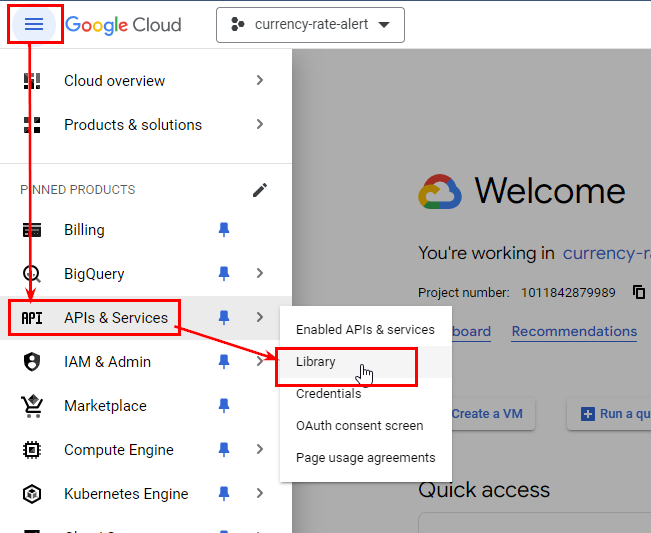
\includegraphics{img/9-1.png}

\subsubsection{Инициализация Google Cloud SDK и настройка Docker}\label{ux438ux43dux438ux446ux438ux430ux43bux438ux437ux430ux446ux438ux44f-google-cloud-sdk-ux438-ux43dux430ux441ux442ux440ux43eux439ux43aux430-docker}

Так же как и в разделе \hyperref[ux43aux430ux43a-ux43dux430ux441ux442ux440ux43eux438ux442ux44c-ux437ux430ux43fux443ux441ux43a-ux441ux43aux440ux438ux43fux442ux430-ux43fux43e-ux440ux430ux441ux441ux43fux438ux441ux430ux43dux438ux44e-ux441-ux43fux43eux43cux43eux449ux44cux44e-google-cloude-run-job]{Как настроить запуск скрипта по рассписанию с помощью Google Cloude Run Job} перед тем как что либо публиковать в Google Cloud нам необходимо там авторизоваться, и настроить Docker на работу с Google Cloud Platform, делается это двумя командами.

\begin{verbatim}
gcloud init
\end{verbatim}

Далее запуститься процесс инициализации, просто следуйте инструкциям, вам необходимо будет пройти авторизацию через браузер, выбрать нужный проект, и указать регион по умолчанию.

Далее необходимо настроить Docker для работы с Google Cloud.

\begin{verbatim}
gcloud auth configure-docker
\end{verbatim}

Если а прошлом шаге вы пропустили процесс активации необходимых API в вашем Google Cloud проекте, то на даном этапе вы можете это сделать прямо из Google Cloud SDK Shell:

\begin{verbatim}
gcloud services enable run.googleapis.com
gcloud services enable artifactregistry.googleapis.com
\end{verbatim}

\subsubsection{Отправка Docker образа в Google Cloud и первый запуск бота}\label{ux43eux442ux43fux440ux430ux432ux43aux430-docker-ux43eux431ux440ux430ux437ux430-ux432-google-cloud-ux438-ux43fux435ux440ux432ux44bux439-ux437ux430ux43fux443ux441ux43a-ux431ux43eux442ux430}

После успешного локального тестирования мы можем тегировать и отправить наш Docker образ в Google Artifact Registry, для этого выполним следующие команды.

\begin{verbatim}
docker tag curbot gcr.io/[PROJECT ID]/[IMAGE NAME]
docker push gcr.io/[PROJECT ID]/[IMAGE NAME]
\end{verbatim}

Теперь пришло время первого запуска бота, выполняем следующую команду.

\begin{verbatim}
gcloud run deploy [SERVICE NAME] --image gcr.io/[PROJECT ID]/[IMAGE NAME] --platform managed --allow-unauthenticated
\end{verbatim}

В случае успешного запуска в консоли вы увидите подобное сообщение:

\begin{verbatim}
Deploying container to Cloud Run service [SERVICE NAME] in project [PROJECT ID] region [africa-south1]
OK Deploying new service... Done.
OK Creating Revision...
OK Routing traffic...
OK Setting IAM Policy...
Done.
Service [SERVICE NAME] revision [currency-tg-bot-00001-6r2] has been deployed and is serving 100 percent of traffic.
Service URL: https://currency-tg-bot-lmgsq7kjta-bq.a.run.app
\end{verbatim}

Наш бот по прежнему не реагирует на сообщения, поскольку у него прописан неверный webhook URL. На данном этапе нам необходим было просто получить из Google Cloud Service URL нашего бота, который вы можете найти в последней строке сообщения, которое получили после успешного запуска сервиса. Останавливаем бота и копируем это URL, он нам понадобится на следующем шаге.

\begin{verbatim}
gcloud run services delete [SERVICE NAME] --platform managed
\end{verbatim}

\subsubsection{Прописываем правильный Webhook URL и перезапускаем бота}\label{ux43fux440ux43eux43fux438ux441ux44bux432ux430ux435ux43c-ux43fux440ux430ux432ux438ux43bux44cux43dux44bux439-webhook-url-ux438-ux43fux435ux440ux435ux437ux430ux43fux443ux441ux43aux430ux435ux43c-ux431ux43eux442ux430}

Итак, теперь у нас есть Service URL, полученный на прошлом шагу, в моём примере это \url{https://currency-tg-bot-lmgsq7kjta-bq.a.run.app}, для того, что бы из этого URL дслеать рабоичй Webhook URL достаточно просто добавить \texttt{/webhook}. Т.е. редактируем значение переменной \texttt{WEBHOOK\_URL} в нашем Dickorfie:

\begin{Shaded}
\begin{Highlighting}[]
\CommentTok{\# Use the official R base image}
\KeywordTok{FROM}\NormalTok{ rocker/r{-}ver:4.1.0}

\CommentTok{\# Set the shell}
\KeywordTok{SHELL}\NormalTok{ [}\StringTok{"/bin/bash"}\NormalTok{, }\StringTok{"{-}o"}\NormalTok{, }\StringTok{"pipefail"}\NormalTok{, }\StringTok{"{-}e"}\NormalTok{, }\StringTok{"{-}u"}\NormalTok{, }\StringTok{"{-}x"}\NormalTok{, }\StringTok{"{-}c"}\NormalTok{]}

\CommentTok{\# Install necessary system dependencies}
\KeywordTok{USER}\NormalTok{ root}
\KeywordTok{RUN} \ExtensionTok{apt{-}get}\NormalTok{ update }\KeywordTok{\&\&} \ExtensionTok{apt{-}get}\NormalTok{ install }\AttributeTok{{-}y} \DataTypeTok{\textbackslash{}}
\NormalTok{    libcurl4{-}openssl{-}dev }\DataTypeTok{\textbackslash{}}
\NormalTok{    libssl{-}dev }\DataTypeTok{\textbackslash{}}
    \KeywordTok{\&\&} \FunctionTok{rm} \AttributeTok{{-}rf}\NormalTok{ /var/lib/apt/lists/}\PreprocessorTok{*}

\CommentTok{\# Install necessary R packages}
\KeywordTok{RUN} \ExtensionTok{R} \AttributeTok{{-}e} \StringTok{"install.packages(c(\textquotesingle{}httr\textquotesingle{}, \textquotesingle{}jsonlite\textquotesingle{}, \textquotesingle{}httpuv\textquotesingle{}))"}
\KeywordTok{RUN} \ExtensionTok{R} \AttributeTok{{-}e} \StringTok{"install.packages(\textquotesingle{}telegram.bot\textquotesingle{}, repos = \textquotesingle{}http://cran.us.r{-}project.org\textquotesingle{})"}

\KeywordTok{ENV}\NormalTok{ EXCHANGERATE\_API\_KEY=[ВАШ КЛЮЧ В exchangerate{-}api.com]}
\KeywordTok{ENV}\NormalTok{ R\_TELEGRAM\_BOT\_CURBOT=[ТОКЕН ВАШЕГО БОТА]}
\KeywordTok{ENV}\NormalTok{ WEBHOOK\_URL=https://currency{-}tg{-}bot{-}lmgsq7kjta{-}bq.a.run.app/webhook}

\CommentTok{\# Copy the R script to the container}
\KeywordTok{COPY}\NormalTok{ curbot.R /app/curbot.R}

\CommentTok{\# Set the working directory}
\KeywordTok{WORKDIR}\NormalTok{ /app}

\CommentTok{\# Run the R script}
\KeywordTok{CMD}\NormalTok{ [}\StringTok{"Rscript"}\NormalTok{, }\StringTok{"/app/curbot.R"}\NormalTok{]}
\end{Highlighting}
\end{Shaded}

Теперь необходимо локально пересобрать образ, протегировать его, отправить новую версию образа в Google Cloud и запустить на его основе сервис.

\begin{verbatim}
docker build -t [IMAGE NAME] .
docker tag curbot gcr.io/[PROJECT ID]/[IMAGE NAME]
docker push gcr.io/[PROJECT ID]/[IMAGE NAME]
gcloud run deploy [SERVICE NAME] --image gcr.io/[PROJECT ID]/[IMAGE NAME] --platform managed --allow-unauthenticated
\end{verbatim}

Если всё прошло успешно вы вновь получите примерно следующее сообщение:

\begin{verbatim}
Deploying container to Cloud Run service [currency-tg-bot] in project [curbot-430507] region [africa-south1]
OK Deploying new service... Done.
OK Creating Revision...
OK Routing traffic...
OK Setting IAM Policy...
Done.
Service [currency-tg-bot] revision [currency-tg-bot-00001-kqg] has been deployed and is serving 100 percent of traffic.
Service URL: https://currency-tg-bot-lmgsq7kjta-bq.a.run.app
\end{verbatim}

поздравляю, теперь ваш ботразвёрнут на Google Cloud Run Service, и готов к использованию:

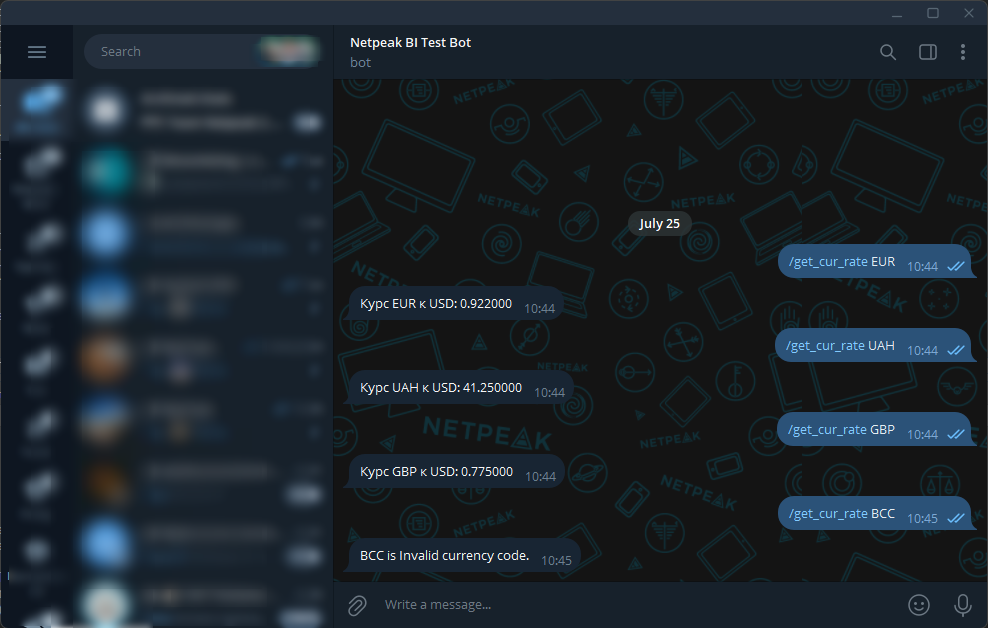
\includegraphics{img/9-9.png}

\section{Heroku}\label{heroku}

Heroku --- это облачный сервис, который помогает разрабатывать, развертывать и управлять веб-приложениями без необходимости заниматься настройкой серверов и инфраструктуры. Вы просто пишете код вашего приложения и отправляете его в Heroku, а система автоматически обрабатывает его развертывание, масштабирование и управление.

Heroku поддерживает разные языки программирования, такие как Ruby, Node.js, Python и в том числе R Она делает процесс разработки проще за счет автоматического развертывания из систем контроля версий (например, Git), управления конфигурацией через переменные среды и возможности добавления различных сервисов, таких как базы данных, через аддоны. Это позволяет разработчикам сосредоточиться на создании функционала, не тратя время на управление серверной инфраструктурой.

Эта платформа подойдёт тем, кто не хочет заморачиваться с Docker, т.к. Heroku имеет специальные buildpacks для различных языков и сред. Для R-скриптов можно использовать buildpack для R, например heroku-buildpack-r. В этом случае вы просто загружаете ваш код и указываете необходимые зависимости в файлах, таких как init.R и Procfile.

\subsection{Разворачиваем telegram бота на Heroku}\label{ux440ux430ux437ux432ux43eux440ux430ux447ux438ux432ux430ux435ux43c-telegram-ux431ux43eux442ux430-ux43dux430-heroku}

\subsubsection{Видео}\label{ux432ux438ux434ux435ux43e-2}

\subsubsection{Обзор рабочего процесса}\label{ux43eux431ux437ux43eux440-ux440ux430ux431ux43eux447ux435ux433ux43e-ux43fux440ux43eux446ux435ux441ux441ux430-2}

Рабочий процесс по развёртыванию ваших ботов на платформе Heroku выглядит следующим образом.

\begin{enumerate}
\def\labelenumi{\arabic{enumi}.}
\tightlist
\item
  Напишите код вашего бота.
\item
  Добавьте в проект остальные необходимые файлы такие как: \texttt{Procfile}, \texttt{init.R}, \texttt{app.json}.
\item
  Зарегистрируйтесь на \href{https://heroku.com}{Heroku}.
\item
  Скачайте и установите утилиту \href{https://devcenter.heroku.com/articles/heroku-cli}{Heroku CLI}.
\item
  Далее вся работа происходит в командной строке, для начала необходимо авторизоваться.
\item
  Перейдите в папку вашего проекта и инициализируйте новый репозиторий Git.
\item
  Создайте коммит со всеми изменениями.
\item
  Добавьте изменения в рабочем каталоге в индекс (или stage area), чтобы они были включены в следующий коммит.
\item
  Создайте новое приложение в Heroku.
\item
  Запросите информацию о вашем приложение, что бы получить его URL.
\item
  Создайте в приложении все необходимые перменные среды.
\item
  Установите нужный buildpack для вашего приложения.
\item
  Отправьте созданный ранее коммит на сервер Heroku и разверните приложение.
\item
  Запустите рабочий процесс приложения.
\end{enumerate}

\subsubsection{Файлы необходимые для разворачиваня бота}\label{ux444ux430ux439ux43bux44b-ux43dux435ux43eux431ux445ux43eux434ux438ux43cux44bux435-ux434ux43bux44f-ux440ux430ux437ux432ux43eux440ux430ux447ux438ux432ux430ux43dux44f-ux431ux43eux442ux430}

Для того, что бы Heroku понял, что ваш бот написан на языке R проекте должен присутствовать хотя бы один из ниже перечисленных файлов:

\begin{itemize}
\tightlist
\item
  \texttt{init.R}
\item
  \texttt{packrat/init/R}
\item
  \texttt{renv/activate.R}
\item
  \texttt{run.R}
\item
  \texttt{app.R}
\item
  \texttt{plumber.R}
\end{itemize}

Файлы app.R и plumber.R характерны соответвенно для Shiny приложений, и API написанных с помощью пакета Plumber. В нашем случае нам пондобятся следующие файлы в проекте бота:

\begin{itemize}
\tightlist
\item
  \texttt{bot.R} - код самого бота
\item
  \texttt{Procfile} - Описание процесса, который будет запускаться в нашем приложении.
\item
  \texttt{init.R} - Описание зависимостей, т.е. пакетов, которые необходимо установить для работы кода нашего бота, так же вы можете использовать более продвинутые техники управления зависимостями (пакеты \texttt{pacrat} или \texttt{renv}).
\item
  \texttt{app.json} (опционально) - Используется для автоматизации процесса развертывания и описания приложения в рамках Heroku.
\end{itemize}

Мы будем разворачивать того же бота, что и в предыдущем разделе, его код выглядит следующим образом:

\begin{Shaded}
\begin{Highlighting}[]
\FunctionTok{library}\NormalTok{(telegram.bot)}
\FunctionTok{library}\NormalTok{(httr)}
\FunctionTok{library}\NormalTok{(jsonlite)}

\CommentTok{\# Метод запроса курса валют}
\NormalTok{get\_cur\_rate }\OtherTok{\textless{}{-}} \ControlFlowTok{function}\NormalTok{(bot, update, args) \{}
  
\NormalTok{  currency\_code }\OtherTok{\textless{}{-}} \FunctionTok{toupper}\NormalTok{(args)}
\NormalTok{  api\_key }\OtherTok{\textless{}{-}} \FunctionTok{Sys.getenv}\NormalTok{(}\StringTok{\textquotesingle{}EXCHANGERATE\_API\_KEY\textquotesingle{}}\NormalTok{)}
\NormalTok{  url     }\OtherTok{\textless{}{-}} \FunctionTok{paste0}\NormalTok{(}\StringTok{"https://api.exchangerate{-}api.com/v4/latest/USD?apikey="}\NormalTok{, api\_key)}
  
\NormalTok{  response }\OtherTok{\textless{}{-}} \FunctionTok{GET}\NormalTok{(url)}
\NormalTok{  data }\OtherTok{\textless{}{-}} \FunctionTok{fromJSON}\NormalTok{(}\FunctionTok{content}\NormalTok{(response, }\StringTok{"text"}\NormalTok{))}
  
  \ControlFlowTok{if}\NormalTok{ (}\SpecialCharTok{!}\NormalTok{currency\_code }\SpecialCharTok{\%in\%} \FunctionTok{names}\NormalTok{(data}\SpecialCharTok{$}\NormalTok{rates)) \{}
\NormalTok{    bot}\SpecialCharTok{$}\FunctionTok{sendMessage}\NormalTok{(}\AttributeTok{chat\_id =}\NormalTok{ update}\SpecialCharTok{$}\NormalTok{message}\SpecialCharTok{$}\NormalTok{chat\_id, }\AttributeTok{text =} \FunctionTok{paste0}\NormalTok{(args, }\StringTok{" is Invalid currency code."}\NormalTok{))}
    \FunctionTok{return}\NormalTok{(}\ConstantTok{NULL}\NormalTok{)}
\NormalTok{  \}}
  
\NormalTok{  rate }\OtherTok{\textless{}{-}}\NormalTok{ data}\SpecialCharTok{$}\NormalTok{rates[[currency\_code]]}
\NormalTok{  message }\OtherTok{\textless{}{-}} \FunctionTok{sprintf}\NormalTok{(}\StringTok{"Курс \%s к USD: \%f"}\NormalTok{, currency\_code, rate)}
\NormalTok{  bot}\SpecialCharTok{$}\FunctionTok{sendMessage}\NormalTok{(}\AttributeTok{chat\_id =}\NormalTok{ update}\SpecialCharTok{$}\NormalTok{message}\SpecialCharTok{$}\NormalTok{chat\_id, }\AttributeTok{text =}\NormalTok{ message)}
  
\NormalTok{\}}

\CommentTok{\# Создаём Webhook}
\NormalTok{webhook }\OtherTok{\textless{}{-}} \FunctionTok{Webhook}\NormalTok{(}
  \AttributeTok{webhook\_url =} \FunctionTok{Sys.getenv}\NormalTok{(}\StringTok{\textquotesingle{}WEBHOOK\_URL\textquotesingle{}}\NormalTok{), }
  \AttributeTok{token       =} \FunctionTok{bot\_token}\NormalTok{(}\StringTok{\textquotesingle{}CURBOT\textquotesingle{}}\NormalTok{), }
  \AttributeTok{verbose     =} \ConstantTok{TRUE}
\NormalTok{  )}

\CommentTok{\# Добавляем обработчики}
\NormalTok{webhook }\OtherTok{\textless{}{-}}\NormalTok{ webhook }\SpecialCharTok{+} \FunctionTok{CommandHandler}\NormalTok{(}\StringTok{"get\_cur\_rate"}\NormalTok{, get\_cur\_rate, }\AttributeTok{pass\_args =}\NormalTok{ T)}

\CommentTok{\# Запускаем Webhook}
\NormalTok{webhook}\SpecialCharTok{$}\FunctionTok{start\_server}\NormalTok{(}
  \AttributeTok{host =} \StringTok{"0.0.0.0"}\NormalTok{,}
  \AttributeTok{port =} \FunctionTok{as.integer}\NormalTok{(}\FunctionTok{Sys.getenv}\NormalTok{(}\StringTok{"PORT"}\NormalTok{, }\DecValTok{8080}\NormalTok{))}
\NormalTok{)}
\end{Highlighting}
\end{Shaded}

Единственное отличае от кода бота приведённого в прошлом разделе это то, что порт мы получаем из переменной среды \texttt{Sys.getenv("PORT",\ 8080)}. Т.к. Heroku назначит случайный порт для вашего приложения, а Google Cloud всегда назначает вашему боту порт 8080.

\texttt{Procfile} используется Heroku для определения процесса, который будет запущен для вашего приложения. Это специальный файл, который указывает, какие команды нужно выполнять при запуске приложения.

\begin{verbatim}
web: R --file=bot.R
\end{verbatim}

\begin{itemize}
\tightlist
\item
  web --- это тип процесса. Для веб-приложений на Heroku это обычно web, и Heroku ожидает, что этот процесс будет слушать входящие HTTP-запросы.
\item
  \texttt{R\ -\/-file=bot.R} --- это команда, которая будет запущена Heroku для старта вашего приложения. Она указывает на то, что нужно выполнить скрипт из файла bot.R.
\end{itemize}

Файл \texttt{init.R} используется для установки пакетов R по мере необходимости.

\begin{quote}
ПРИМЕЧАНИЕ: Использование Packrat или renv --- лучший способ управления зависимостями пакетов и их соответствующими версиями, поэтому этот init.Rфайл не требуется, если вы используете packratили renv.
\end{quote}

Я использую следующий пример \texttt{init.R} файла:

\begin{Shaded}
\begin{Highlighting}[]
\FunctionTok{helpers.installPackages}\NormalTok{(}\StringTok{"httr"}\NormalTok{, }\StringTok{"jsonlite"}\NormalTok{, }\StringTok{"telegram.bot"}\NormalTok{, }\StringTok{"stringr"}\NormalTok{)}
\end{Highlighting}
\end{Shaded}

Вспомогательная функция \texttt{helpers.installPackages}, упрощающая установку пакетов, включена в buildpack для удобства.

Файл \texttt{app.json} используется для автоматизации процесса развертывания и описания приложения в рамках Heroku. Это полезно для использования с Heroku Review Apps и автоматическим развертыванием.

\begin{Shaded}
\begin{Highlighting}[]
\FunctionTok{\{}
  \DataTypeTok{"name"}\FunctionTok{:} \StringTok{"telegram{-}bot"}\FunctionTok{,}
  \DataTypeTok{"description"}\FunctionTok{:} \StringTok{"A Telegram bot deployed on Heroku"}\FunctionTok{,}
  \DataTypeTok{"repository"}\FunctionTok{:} \StringTok{"https://github.com/your{-}repo/your{-}bot{-}repo"}\FunctionTok{,}
  \DataTypeTok{"logo"}\FunctionTok{:} \StringTok{"https://example.com/logo.png"}\FunctionTok{,}
  \DataTypeTok{"keywords"}\FunctionTok{:} \OtherTok{[}\StringTok{"telegram"}\OtherTok{,} \StringTok{"bot"}\OtherTok{]}\FunctionTok{,}
  \DataTypeTok{"env"}\FunctionTok{:} \FunctionTok{\{}
    \DataTypeTok{"R\_TELEGRAM\_BOT\_CURBOT"}\FunctionTok{:} \FunctionTok{\{}
      \DataTypeTok{"description"}\FunctionTok{:} \StringTok{"Telegram Bot Token"}\FunctionTok{,}
      \DataTypeTok{"required"}\FunctionTok{:} \KeywordTok{true}
    \FunctionTok{\},}
    \DataTypeTok{"EXCHANGERATE\_API\_KEY"}\FunctionTok{:} \FunctionTok{\{}
      \DataTypeTok{"description"}\FunctionTok{:} \StringTok{"Exchangerate api key"}\FunctionTok{,}
      \DataTypeTok{"required"}\FunctionTok{:} \KeywordTok{true}
    \FunctionTok{\},}
    \DataTypeTok{"WEBHOOK\_URL"}\FunctionTok{:} \FunctionTok{\{}
      \DataTypeTok{"description"}\FunctionTok{:} \StringTok{"Webhook URL"}\FunctionTok{,}
      \DataTypeTok{"required"}\FunctionTok{:} \KeywordTok{true}
    \FunctionTok{\}}
  \FunctionTok{\},}
  \DataTypeTok{"buildpacks"}\FunctionTok{:} \OtherTok{[}
    \FunctionTok{\{}
      \DataTypeTok{"url"}\FunctionTok{:} \StringTok{"https://github.com/virtualstaticvoid/heroku{-}buildpack{-}r.git"}
    \FunctionTok{\}}
  \OtherTok{]}
\FunctionTok{\}}
\end{Highlighting}
\end{Shaded}

Что это означает:

\begin{itemize}
\tightlist
\item
  ``name'' --- имя вашего приложения на Heroku.
\item
  ``description'' --- краткое описание приложения.
\item
  ``repository'' --- ссылка на репозиторий с вашим кодом.
\item
  ``logo'' --- URL к логотипу вашего приложения.
\item
  ``keywords'' --- ключевые слова для поиска вашего приложения.
\item
  ``env'' --- переменные окружения, которые требуется установить для вашего приложения (например, токен для Telegram API и URL вебхука).
\item
  ``buildpacks'' --- список buildpacks, которые будут использоваться для развертывания. Здесь указан buildpack для R.
\end{itemize}

\subsubsection{Авторизация и инициализация Git репозитория}\label{ux430ux432ux442ux43eux440ux438ux437ux430ux446ux438ux44f-ux438-ux438ux43dux438ux446ux438ux430ux43bux438ux437ux430ux446ux438ux44f-git-ux440ux435ux43fux43eux437ux438ux442ux43eux440ux438ux44f}

Далее для авторизации в командной строке выполняем команду:

\begin{verbatim}
heroku login
\end{verbatim}

После чего необходимо инициализировать новый репозиторий, добавить все изменения и создать коммит.

\begin{verbatim}
git init
git add .
git commit -m "Initial commit"
\end{verbatim}

\begin{itemize}
\tightlist
\item
  \texttt{git\ init} - Эта команда инициализирует новый репозиторий Git в текущей директории. Она создаёт скрытую папку .git, которая содержит всю информацию о версии и конфигурации вашего репозитория. После выполнения этой команды текущая директория становится рабочим репозиторием Git, в котором вы можете отслеживать изменения файлов и выполнять другие операции управления версиями.
\item
  \texttt{git\ add\ .} - Команда git add добавляет изменения в рабочем каталоге в индекс (или stage area), чтобы они были включены в следующий коммит. Аргумент . указывает, что нужно добавить все изменения во всех файлах текущей директории и её поддиректориях. Это делает все текущие изменения подготовленными для следующего коммита.
\item
  \texttt{git\ commit\ -m\ "Initial\ commit"} - Эта команда создает новый коммит в репозитории, включающий все изменения, добавленные в индекс с помощью git add. Флаг -m позволяет указать сообщение коммита прямо в командной строке. Сообщение ``Initial commit'' --- это описание того, что делает этот коммит. Обычно первое сообщение коммита описывает начальную настройку репозитория или первые изменения в проекте.
\end{itemize}

\subsubsection{Создаём новое приложение и запраиваем его URL}\label{ux441ux43eux437ux434ux430ux451ux43c-ux43dux43eux432ux43eux435-ux43fux440ux438ux43bux43eux436ux435ux43dux438ux435-ux438-ux437ux430ux43fux440ux430ux438ux432ux430ux435ux43c-ux435ux433ux43e-url}

Следующая команда создаст в вашем аккаунте Heroku новое приложение:

\begin{verbatim}
heroku create your-app-name
\end{verbatim}

Замените \texttt{your-app-name} на название вашего приложения.

Теперь запросим информацию о приложении, для того что бы получить его URL:

\begin{verbatim}
heroku apps:info
\end{verbatim}

В результате вы получите следующую информацию:

\begin{verbatim}
=== your-app-name

Auto Cert Mgmt: false
Dynos:          web: 1
Git URL:        https://git.heroku.com/your-app-name.git
Owner:          your@gmail.com
Region:         us
Repo Size:      19 KB
Slug Size:      149 MB
Stack:          heroku-22
Web URL:        https://your-app-name-abcdefgh.herokuapp.com/
\end{verbatim}

Из всей этой информации нам понадобится только Web URL, т.к. добавив к его пути webhook, мы получим тот WEBHOOK URL, который нам необходимо будет установить для нашего бота.

\subsubsection{Добавляем переменные среды}\label{ux434ux43eux431ux430ux432ux43bux44fux435ux43c-ux43fux435ux440ux435ux43cux435ux43dux43dux44bux435-ux441ux440ux435ux434ux44b}

В коде нашего бота мы используем 3 переменные среды:

\begin{itemize}
\tightlist
\item
  EXCHANGERATE\_API\_KEY - API Ключ, который вам необходимо получить на сайте exchangerate-api.com
\item
  R\_TELEGRAM\_BOT\_CURBOT - API Token вашего бота, получить его можно при создании бота через \href{https://t.me/BotFather}{BotFather}
\item
  WEBHOOK\_URL - Webhook URL на который telegram будет присылать обновления для бота, берём значение из Web URL нашего приложения, и добавляем webhook, в нашем примере \url{https://your-app-name-abcdefgh.herokuapp.com/webhook}.
\end{itemize}

Теперь с помощью командной строки создадим эти переменные в приложении:

\begin{verbatim}
heroku config:set R_TELEGRAM_BOT_CURBOT=ТОКЕН ВАШЕГО БОТА
heroku config:set WEBHOOK_URL=https://your-app-name-abcdefgh.herokuapp.com/webhook
heroku config:set EXCHANGERATE_API_KEY=Exchangerate API Ключ
\end{verbatim}

\subsubsection{Установка buildpack}\label{ux443ux441ux442ux430ux43dux43eux432ux43aux430-buildpack}

Buildpack --- это инструмент, который автоматически устанавливает и настраивает необходимые зависимости для вашего приложения. Он помогает платформе как определить, как собрать и запустить ваше приложение.

Вот основные моменты, зачем и как он используется:

\begin{itemize}
\tightlist
\item
  \textbf{Автоматическая настройка среды}: Buildpack управляет установкой всех необходимых зависимостей и инструментов, таких как языковые среды (например, Ruby, Python, Node.js), библиотеки и фреймворки. Он автоматически настраивает среду, в которой будет работать ваше приложение, чтобы не нужно было вручную управлять этими процессами.
\item
  \textbf{Определение процесса сборки}: Buildpack предоставляет инструкции о том, как собрать ваше приложение. Например, он может определить, какие команды нужно выполнить для установки зависимостей или как собрать исходный код.
\item
  \textbf{Упрощение развертывания}: С помощью buildpack процесс развертывания становится проще и более автоматизированным. Вы можете просто загрузить свой код, и buildpack позаботится обо всех необходимых шагах для подготовки и запуска приложения.
\item
  \textbf{Поддержка различных языков и фреймворков}: Разные buildpack могут поддерживать разные языки программирования и фреймворки. Например, есть отдельные buildpack для Java, Python, R и других языков.
\end{itemize}

Для использования buildpack в Heroku, вы указываете его при создании или настройке приложения. Например, если вы развертываете приложение на языке R, вам нужен соответствующий buildpack, который знает, как установить R и необходимые пакеты.

Пример использования buildpack в Heroku:

\begin{itemize}
\tightlist
\item
  Установка buildpack: Команда heroku buildpacks:set \url{https://github.com/virtualstaticvoid/heroku-buildpack-r.git} устанавливает buildpack для языка R.
  ( Автоматическая установка зависимостей: При развертывании Heroku использует buildpack для установки R, необходимых библиотек и фреймворков, а затем собирает и запускает ваше приложение.
\end{itemize}

Таким образом, buildpack упрощает процесс развертывания, автоматизируя установку и настройку среды для вашего приложения.

Для установки нужного для языка R buildpack используйте следующую команду:

\begin{verbatim}
heroku buildpacks:set https://github.com/virtualstaticvoid/heroku-buildpack-r.git
\end{verbatim}

\subsubsection{Отправка данных в Heroku и запуск бота}\label{ux43eux442ux43fux440ux430ux432ux43aux430-ux434ux430ux43dux43dux44bux445-ux432-heroku-ux438-ux437ux430ux43fux443ux441ux43a-ux431ux43eux442ux430}

Последним шагом необзодимо отправить все изменения в Heroku и запустить рабочий процесс, делается жто следующими командами:

\begin{verbatim}
git push heroku master
heroku ps:scale web=1
\end{verbatim}

\begin{itemize}
\item
  \textbf{Команда git push heroku master}: Эта команда отправляет ваши файлы проекта на сервер Heroku и разворачивает приложение.
  Она обновляет код вашего приложения в Heroku и выполняет установку зависимостей, но не запускает процесс приложения.
  После выполнения этой команды ваше приложение будет развернуто на Heroku, но может еще не быть активным или не обрабатывать запросы, если не настроены нужные процессы.
\item
  \textbf{Команда heroku ps:scale web=1}: Эта команда запускает веб-процесс для вашего приложения.
  Она указывает Heroku, что нужно запустить один экземпляр веб-процесса, который будет слушать входящие HTTP-запросы.
  После выполнения этой команды ваш бот начнет принимать запросы и будет отвечать на них, если всё настроено правильно.
\end{itemize}

Таким образом, после \texttt{git\ push\ heroku\ master} ваше приложение будет развернуто, но вам нужно выполнить \texttt{heroku\ ps:scale\ web=1}, чтобы запустить его и начать обработку запросов.

Всё, ваш бот развёрнут на Heroku!

\subsubsection{Переключение между разными приложениями}\label{ux43fux435ux440ux435ux43aux43bux44eux447ux435ux43dux438ux435-ux43cux435ux436ux434ux443-ux440ux430ux437ux43dux44bux43cux438-ux43fux440ux438ux43bux43eux436ux435ux43dux438ux44fux43cux438}

В heroku у вас могут быть созданы несколько приложений, если вам необходимо будет переключаться между ними, то можете воспользоваться следующими командами:

\begin{itemize}
\tightlist
\item
  \texttt{heroku\ apps} - Эта команда покажет все ваши приложения в Heroku.
\item
  \texttt{heroku\ git:remote\ -a\ \textless{}app\_name\textgreater{}} - Для переключения между приложениями.
\end{itemize}

В некоторых командах можно указать имя приложения, используя флаг -a:

\begin{itemize}
\tightlist
\item
  \texttt{heroku\ ps\ -a\ \textless{}app\_name\textgreater{}}
\item
  \texttt{heroku\ logs\ -\/-tail\ -a\ \textless{}app\_name\textgreater{}}
\item
  \texttt{heroku\ ps:scale\ web=1\ -a\ \textless{}app\_name\textgreater{}}
\item
  \texttt{heroku\ config:set\ VAR\_NAME=value\ -a\ \textless{}app\_name\textgreater{}}
\end{itemize}

\subsubsection{Другие полезные команды Heroku cli}\label{ux434ux440ux443ux433ux438ux435-ux43fux43eux43bux435ux437ux43dux44bux435-ux43aux43eux43cux430ux43dux434ux44b-heroku-cli}

Вот ещё несколько полезных команд, доступных в Heroku CLI:

\begin{itemize}
\tightlist
\item
  \texttt{heroku\ ps} - отображения текущего состояния процессов (dynos) вашего приложения
\item
  \texttt{heroku\ config} - просмотр переменных
\item
  \texttt{heroku\ apps:info} - получить инфу о приложении, включая его url
\item
  \texttt{heroku\ logs\ -\/-tail} - покажет логи выполнения R скрипта
\end{itemize}

\subsection{Как настроить запуск R скрипта по расписанию в Heroku}\label{ux43aux430ux43a-ux43dux430ux441ux442ux440ux43eux438ux442ux44c-ux437ux430ux43fux443ux441ux43a-r-ux441ux43aux440ux438ux43fux442ux430-ux43fux43e-ux440ux430ux441ux43fux438ux441ux430ux43dux438ux44e-ux432-heroku}

На предыдущем шаге мы развернули в Heroku полноценного бота, но возможно вам необходимо просто настроить отправку какого либо сообщение в telegtam по расписанию. Алгоритм очень похож с развёртыванием бота, но всё таки он немного упрощён.

\subsubsection{Подготовка проекта}\label{ux43fux43eux434ux433ux43eux442ux43eux432ux43aux430-ux43fux440ux43eux435ux43aux442ux430}

Мы будем разворачивать тот же скрипт, отправляющий курсы валют, который рассматривали в разеделе \hyperref[ux43aux430ux43a-ux43dux430ux441ux442ux440ux43eux438ux442ux44c-ux437ux430ux43fux443ux441ux43a-ux441ux43aux440ux438ux43fux442ux430-ux43fux43e-ux440ux430ux441ux441ux43fux438ux441ux430ux43dux438ux44e-ux441-ux43fux43eux43cux43eux449ux44cux44e-google-cloude-run-job]{Как настроить запуск скрипта по рассписанию с помощью Google Cloude Run Job}:

Файл init.R:

\begin{Shaded}
\begin{Highlighting}[]
\FunctionTok{helpers.installPackages}\NormalTok{(}\StringTok{"httr"}\NormalTok{, }\StringTok{"jsonlite"}\NormalTok{, }\StringTok{"telegram.bot"}\NormalTok{, }\StringTok{"stringr"}\NormalTok{)}
\end{Highlighting}
\end{Shaded}

Файл script.R:

\begin{Shaded}
\begin{Highlighting}[]
\FunctionTok{library}\NormalTok{(httr)}
\FunctionTok{library}\NormalTok{(jsonlite)}
\FunctionTok{library}\NormalTok{(telegram.bot)}
\FunctionTok{library}\NormalTok{(stringr)}

\NormalTok{get\_exchange\_rate }\OtherTok{\textless{}{-}} \ControlFlowTok{function}\NormalTok{(api\_key) \{}
\NormalTok{  url }\OtherTok{\textless{}{-}} \FunctionTok{paste0}\NormalTok{(}\StringTok{"https://api.exchangerate{-}api.com/v4/latest/USD?apikey="}\NormalTok{, api\_key)}
\NormalTok{  response }\OtherTok{\textless{}{-}} \FunctionTok{GET}\NormalTok{(url)}
\NormalTok{  data }\OtherTok{\textless{}{-}} \FunctionTok{fromJSON}\NormalTok{(}\FunctionTok{content}\NormalTok{(response, }\StringTok{"text"}\NormalTok{))}
  \FunctionTok{return}\NormalTok{(data)}
\NormalTok{\}}

\NormalTok{send\_telegram\_message }\OtherTok{\textless{}{-}} \ControlFlowTok{function}\NormalTok{(bot\_token, chat\_id, message) \{}
\NormalTok{  bot }\OtherTok{\textless{}{-}} \FunctionTok{Bot}\NormalTok{(}\AttributeTok{token =}\NormalTok{ bot\_token)}
\NormalTok{  bot}\SpecialCharTok{$}\FunctionTok{sendMessage}\NormalTok{(}\AttributeTok{chat\_id =}\NormalTok{ chat\_id, }\AttributeTok{text =}\NormalTok{ message)}
\NormalTok{\}}

\CommentTok{\# Функция для выполнения основного логики}
\NormalTok{execute\_script }\OtherTok{\textless{}{-}} \ControlFlowTok{function}\NormalTok{() \{}
\NormalTok{  api\_key   }\OtherTok{\textless{}{-}} \FunctionTok{Sys.getenv}\NormalTok{(}\StringTok{"EXCHANGE\_RATE\_API\_KEY"}\NormalTok{)}
\NormalTok{  bot\_token }\OtherTok{\textless{}{-}} \FunctionTok{Sys.getenv}\NormalTok{(}\StringTok{"TELEGRAM\_BOT\_TOKEN"}\NormalTok{)}
\NormalTok{  chat\_id   }\OtherTok{\textless{}{-}} \FunctionTok{Sys.getenv}\NormalTok{(}\StringTok{"TELEGRAM\_CHAT\_ID"}\NormalTok{)}
  
\NormalTok{  exchange\_rate }\OtherTok{\textless{}{-}} \FunctionTok{get\_exchange\_rate}\NormalTok{(api\_key)}
\NormalTok{  message }\OtherTok{\textless{}{-}} \FunctionTok{str\_glue}\NormalTok{(}
    \StringTok{"Курс валют на \{Sys.Date()\}"}\NormalTok{,}
    \StringTok{\textquotesingle{}{-}{-}{-}{-}{-}{-}{-}{-}{-}{-}{-}{-}{-}{-}{-}{-}{-}{-}{-}{-}{-}{-}{-}{-}{-}{-}{-}{-}{-}\textquotesingle{}}\NormalTok{,}
    \StringTok{"Курс EUR к USD: \{exchange\_rate$rates$EUR\}"}\NormalTok{, }
    \StringTok{"Курс GBP к USD: \{exchange\_rate$rates$GBP\}"}\NormalTok{,}
    \StringTok{"Курс UAH к USD: \{exchange\_rate$rates$UAH\}"}\NormalTok{,}
    \StringTok{"Курс EGP к USD: \{exchange\_rate$rates$EGP\}"}\NormalTok{, }
    \AttributeTok{.sep =} \StringTok{\textquotesingle{}}\SpecialCharTok{\textbackslash{}n}\StringTok{\textquotesingle{}}
\NormalTok{  )}
  
  \FunctionTok{send\_telegram\_message}\NormalTok{(bot\_token, chat\_id, message)}
\NormalTok{\}}

\CommentTok{\# Выполнение скрипта}
\FunctionTok{execute\_script}\NormalTok{()}
\end{Highlighting}
\end{Shaded}

\subsubsection{Обзор рабочего процесса}\label{ux43eux431ux437ux43eux440-ux440ux430ux431ux43eux447ux435ux433ux43e-ux43fux440ux43eux446ux435ux441ux441ux430-3}

\begin{enumerate}
\def\labelenumi{\arabic{enumi}.}
\tightlist
\item
  В вашем приложение достаточно двух файлов:

  \begin{enumerate}
  \def\labelenumii{\arabic{enumii}.}
  \tightlist
  \item
    init.R с описанием зависимосте.
  \item
    script.R, ну или любой файл с R кодом, который вам необходимо запускать по расписанию.
  \end{enumerate}
\item
  Залогиньтесь в Heroku, и подготовьте коммит:
\end{enumerate}

\begin{verbatim}
heroku login

git init
git add .
git commit -m "Initial commit"
\end{verbatim}

\begin{enumerate}
\def\labelenumi{\arabic{enumi}.}
\setcounter{enumi}{2}
\tightlist
\item
  Создайте приложение
\end{enumerate}

\begin{verbatim}
heroku create app-name
\end{verbatim}

\begin{enumerate}
\def\labelenumi{\arabic{enumi}.}
\setcounter{enumi}{3}
\tightlist
\item
  Создайте все необходимые переменные среды:
\end{enumerate}

\begin{verbatim}
heroku config:set EXCHANGE_RATE_API_KEY=<ВАШ КЛЮЧ К exchange-rate-api>
heroku config:set TELEGRAM_BOT_TOKEN=<ТОКЕН ВАШЕГО БОТА>
heroku config:set TELEGRAM_CHAT_ID=<ID чата в который будете отправлять курсы валют>
\end{verbatim}

\begin{enumerate}
\def\labelenumi{\arabic{enumi}.}
\setcounter{enumi}{4}
\tightlist
\item
  Устновите нужный buildpack:
\end{enumerate}

\begin{verbatim}
heroku buildpacks:set https://github.com/virtualstaticvoid/heroku-buildpack-r.git
\end{verbatim}

\begin{enumerate}
\def\labelenumi{\arabic{enumi}.}
\setcounter{enumi}{5}
\tightlist
\item
  Запушьте приложение
\end{enumerate}

\begin{verbatim}
git push heroku master
\end{verbatim}

\begin{enumerate}
\def\labelenumi{\arabic{enumi}.}
\setcounter{enumi}{6}
\tightlist
\item
  Перейдите в web версию \href{https://heroku.com}{Heroku}, зайдите в созданное приложение, перейдите на вкладку Resources? и добавьте Add-on ``Heroku Scheduler'', есть и другие дополнения, которые позволяют настраивать расписание запуска ваших скриптов, но они платные:
\end{enumerate}

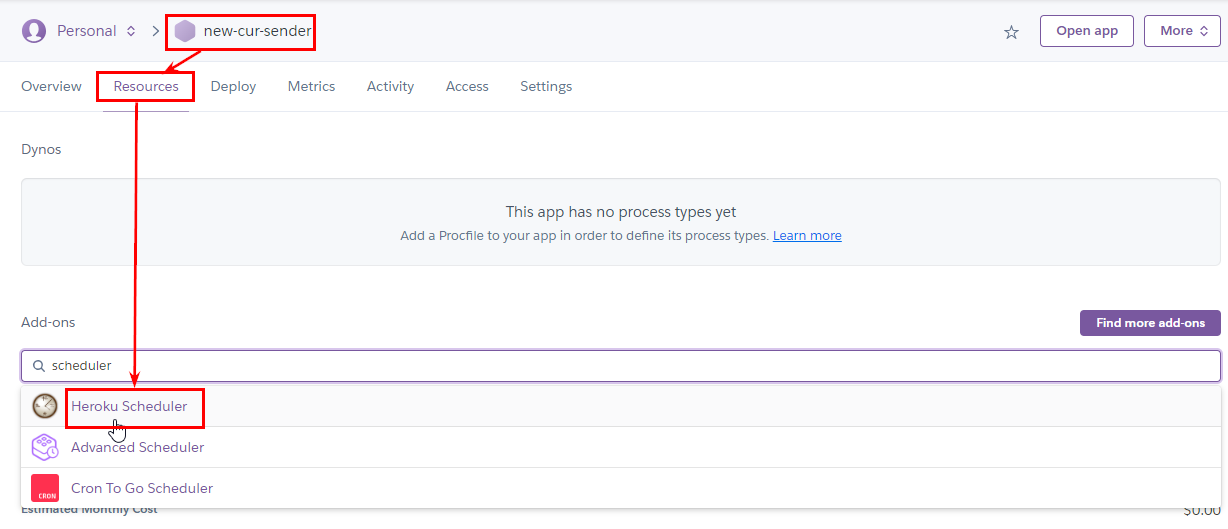
\includegraphics{img/9-10.png}

\begin{enumerate}
\def\labelenumi{\arabic{enumi}.}
\setcounter{enumi}{7}
\tightlist
\item
  Перейдите в дополннеие ``Heroku Scheduler'' и нажмите ``Create job''
\end{enumerate}

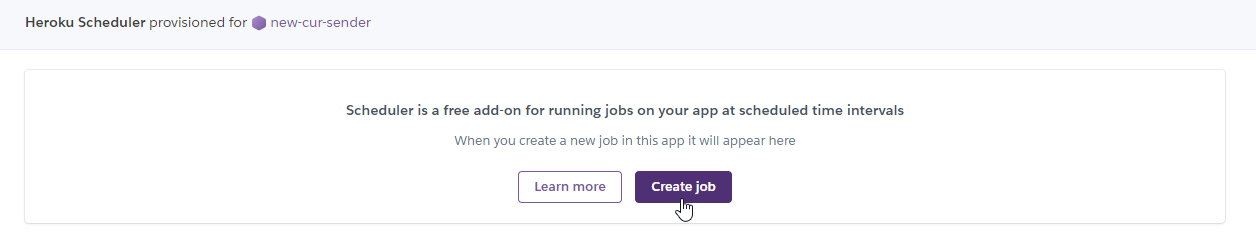
\includegraphics{img/9-11.png}

\begin{enumerate}
\def\labelenumi{\arabic{enumi}.}
\setcounter{enumi}{8}
\tightlist
\item
  Настройте расписание запуска, и укажите команду \texttt{Rscript\ script.R}:
\end{enumerate}

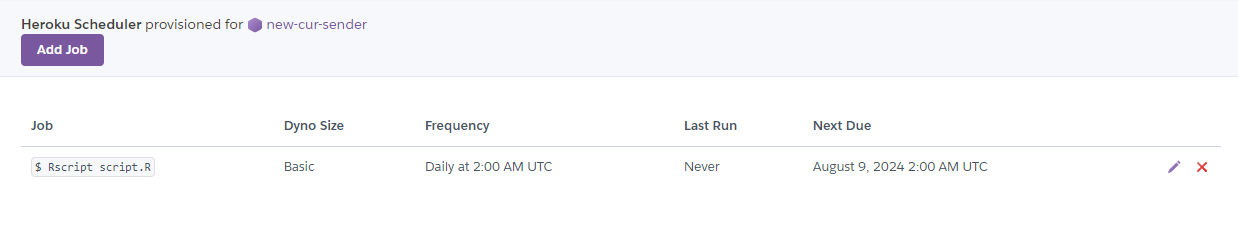
\includegraphics{img/9-12.png}

Возможности настройки расписания в дополнении ``Heroku Scheduler'' довольно примитывные, но можно настроить запуск каждый 10 минут, каждый час в определённую минуту, или каждый день в определённое время.

\section{Какую из описанных облачных платформ выбрать}\label{ux43aux430ux43aux443ux44e-ux438ux437-ux43eux43fux438ux441ux430ux43dux43dux44bux445-ux43eux431ux43bux430ux447ux43dux44bux445-ux43fux43bux430ux442ux444ux43eux440ux43c-ux432ux44bux431ux440ux430ux442ux44c}

Развёртывание бота на Heroku и Google Cloud Run имеет свои особенности и преимущества, в зависимости от ваших требований и предпочтений. Вот некоторые ключевые моменты, которые могут помочь вам определиться:

\subsection{Преимущества Heroku}\label{ux43fux440ux435ux438ux43cux443ux449ux435ux441ux442ux432ux430-heroku}

\begin{enumerate}
\def\labelenumi{\arabic{enumi}.}
\tightlist
\item
  \textbf{Простота и удобство использования:}

  \begin{itemize}
  \tightlist
  \item
    Интуитивный интерфейс: Heroku предлагает простой в использовании интерфейс и инструменты командной строки, которые облегчают развертывание и управление приложениями.
  \item
    Автоматическое масштабирование: Heroku автоматически масштабирует ваше приложение в зависимости от нагрузки, и вам не нужно заботиться о настройке серверов.
  \end{itemize}
\item
  \textbf{Широкий выбор buildpack и добавок:}

  \begin{itemize}
  \tightlist
  \item
    Buildpacks: Heroku поддерживает различные языковые среды через buildpacks, что упрощает настройку среды для вашего приложения.
  \item
    Дополнения: В магазине расширений Heroku можно найти множество сервисов для мониторинга, баз данных, очередей и других нужд.
  \end{itemize}
\item
  \textbf{Автоматическое управление зависимостями:}

  \begin{itemize}
  \tightlist
  \item
    Легкость в управлении: Heroku автоматически управляет зависимостями и настройками окружения, что упрощает развертывание.
  \end{itemize}
\item
  \textbf{Встроенные инструменты для мониторинга и логирования:}

  \begin{itemize}
  \tightlist
  \item
    Логи и мониторинг: Heroku предоставляет встроенные инструменты для мониторинга и сбора логов, что помогает отслеживать состояние вашего приложения.
  \end{itemize}
\item
  \textbf{Интеграция с Git:}

  \begin{itemize}
  \tightlist
  \item
    Git-процесс: Простая интеграция с Git позволяет использовать стандартные git-команды для развертывания и обновления приложений.
  \end{itemize}
\end{enumerate}

\subsection{Преимущества Google Cloud Run}\label{ux43fux440ux435ux438ux43cux443ux449ux435ux441ux442ux432ux430-google-cloud-run}

\begin{enumerate}
\def\labelenumi{\arabic{enumi}.}
\tightlist
\item
  \textbf{Масштабируемость и гибкость:}

  \begin{itemize}
  \tightlist
  \item
    Масштабируемость: Google Cloud Run автоматически масштабирует ваше приложение в зависимости от входящих запросов и может обрабатывать трафик от нуля до тысяч запросов в секунду.
  \item
    Гибкость: Поддержка контейнеров позволяет вам использовать любой язык программирования и фреймворк, который вы хотите.
  \end{itemize}
\item
  \textbf{Полный контроль над окружением:}

  \begin{itemize}
  \tightlist
  \item
    Контейнеры: Вы можете использовать Docker-контейнеры, что дает вам полный контроль над средой выполнения вашего приложения, включая версии зависимостей и настройки.
  \end{itemize}
\item
  \textbf{Интеграция с другими сервисами Google Cloud:}

  \begin{itemize}
  \tightlist
  \item
    Богатая экосистема: Cloud Run легко интегрируется с другими сервисами Google Cloud, такими как Cloud SQL, Pub/Sub и Cloud Storage.
  \end{itemize}
\item
  \textbf{Биллинг по запросам:}

  \begin{itemize}
  \tightlist
  \item
    Оплата за использование: Вы оплачиваете только фактическое время работы вашего приложения и количество обработанных запросов, что может быть более экономичным при низкой активности.
  \end{itemize}
\item
  \textbf{Быстрое развертывание и обновление:}

  \begin{itemize}
  \tightlist
  \item
    Контейнеры: С использованием контейнеров вы можете быстро развернуть и обновить приложение, что упрощает управление версиями и деплой.
  \end{itemize}
\end{enumerate}

\subsection{Итог}\label{ux438ux442ux43eux433}

\begin{itemize}
\tightlist
\item
  Heroku лучше подходит для разработчиков, которые ищут простоту и удобство в развертывании, особенно если вы используете стандартные языки программирования и фреймворки, поддерживаемые Heroku. Он хорош для быстрого старта и имеет много встроенных функций и добавок.
\item
  Google Cloud Run предоставит больше гибкости и масштабируемости, особенно если вам нужен полный контроль над средой выполнения или если ваше приложение должно работать в контейнерах. Это хороший выбор для масштабируемых приложений с высокой нагрузкой.
\end{itemize}

Выбор между Heroku и Google Cloud Run зависит от ваших требований к проекту и предпочтений в управлении приложением.

\section{Заключение}\label{ux437ux430ux43aux43bux44eux447ux435ux43dux438ux435-8}

Поздравляю с завершением последней главы! Вы успешно развернули своего бота на Google Cloud Run и готовы к его масштабированию и поддержке в облаке. Надеюсь, вы получили все необходимые знания и навыки для успешного управления и развития вашего бота. Спасибо за участие в этом путешествии, и я надеюсь, что вы продолжите развиваться в мире разработки и анализа данных.

\chapter*{Заключение}\label{ux437ux430ux43aux43bux44eux447ux435ux43dux438ux435-9}
\addcontentsline{toc}{chapter}{Заключение}

Поздравляю вас с завершением нашего путешествия в мир разработки Telegram-ботов с использованием языка R! Мы прошли через все этапы создания и настройки бота, от самых основ до сложных аспектов развертывания и масштабирования. Надеюсь, что вы нашли эту книгу полезной и вдохновляющей, и теперь обладаете всеми необходимыми знаниями для создания и управления собственными ботами.

В ходе этой книги мы:

\begin{enumerate}
\def\labelenumi{\arabic{enumi}.}
\tightlist
\item
  \textbf{Создали и настроили вашего первого бота}: Вы узнали, как использовать API Telegram для запуска простого бота, который может взаимодействовать с пользователями и выполнять базовые функции.
\item
  \textbf{Добавили команды и фильтры}: Мы рассмотрели, как настраивать команды для управления ботом и фильтры для обработки сообщений, чтобы бот мог эффективно выполнять задачи.
\item
  \textbf{Настроили клавиатуры}: Вы изучили, как интегрировать reply и inline клавиатуры для создания интерактивных элементов, которые облегчают взаимодействие с пользователями.
\item
  \textbf{Построили диалоги}: Мы разобрали методы создания сложных последовательностей диалогов для более естественного общения и улучшения понимания запросов пользователей.
\item
  \textbf{Управляли правами пользователей}: Вы узнали, как настраивать права доступа для различных пользователей, обеспечивая безопасность и контроль над взаимодействием с вашим ботом.
\item
  \textbf{Повысили стабильность}: Мы обсудили методы повышения надежности бота, включая обработку ошибок и оптимизацию производительности.
\item
  \textbf{Внедрили асинхронные операции}: Вы научились использовать асинхронность для повышения производительности и масштабируемости вашего бота.
\item
  \textbf{Упаковали бота в Docker}: Мы рассмотрели, как создать Docker-контейнер для удобного развертывания и управления окружением бота.
\item
  \textbf{Развернули бота на Google Cloud Run}: В завершение, мы изучили, как развернуть бота на облачной платформе для обеспечения его масштабируемости и доступности.
\end{enumerate}

Теперь, когда вы освоили все эти аспекты, у вас есть отличная база для создания и управления Telegram-ботами, которые могут выполнять сложные задачи и взаимодействовать с пользователями на высоком уровне. Ваши знания и навыки позволят вам разрабатывать ботов для различных целей, от простых автоматизаций до сложных интерактивных решений.

Не забывайте, что процесс разработки не заканчивается на развертывании. Постоянное совершенствование, тестирование и обновление --- важные части успешного проекта. Надеюсь, что вы продолжите исследовать новые возможности и применять полученные знания для создания ещё более мощных и эффективных решений.

Если вам понравилась эта книга, я буду рад, если вы подпишетесь на мой \href{https://t.me/R4marketing}{Telegram} и \href{https://www.youtube.com/R4marketing/?sub_confirmation=1}{YouTube} каналы R4marketing. На них я делюсь множеством полезных материалов по разработке и анализу данных на языке R, которые помогут вам дальше развиваться в этой области.

Кроме того, вы можете быть заинтересованы в других моих курсах, таких как:

\begin{itemize}
\tightlist
\item
  \href{https://selesnow.github.io/r4excel_users/}{Язык R для пользователей Excel}.
\item
  \href{https://selesnow.github.io/dplyr_1_0_0_course/}{Введение в dplyr 1.0.0}.
\item
  \href{https://selesnow.github.io/iterations_in_r/}{Циклы и функционалы в языке R}.
\item
  \href{https://selesnow.github.io/r_package_course/}{Разработка пакетов на языке R}.
\item
  \href{https://www.youtube.com/playlist?list=PLD2LDq8edf4o6dSZ4BIr7J08gT97nimH_}{Язык R для интернет-маркетинга}.
\end{itemize}

Спасибо, что выбрали эту книгу в качестве своего учебного пособия. Желаю вам удачи в ваших будущих проектах и не прекращайте учиться и развиваться в мире технологий!

{}

\chapter*{Обновления}\label{ux43eux431ux43dux43eux432ux43bux435ux43dux438ux44f}
\addcontentsline{toc}{chapter}{Обновления}

\section*{2025-04-27}\label{section}
\addcontentsline{toc}{section}{2025-04-27}

\begin{itemize}
\tightlist
\item
  В главе \hyperref[ux434ux43eux431ux430ux432ux43bux44fux435ux43c-ux431ux43eux442ux443-ux43fux43eux434ux434ux435ux440ux436ux43aux443-ux43aux43eux43cux430ux43dux434-ux438-ux444ux438ux43bux44cux442ux440ux44b-ux441ux43eux43eux431ux449ux435ux43dux438ux439-ux43aux43bux430ux441ux441-updater]{Добавляем боту поддержку команд и фильтры сообщений, класс Updater} расширен раздел \hyperref[ux437ux430ux43fux443ux441ux43aux430ux435ux43c-ux431ux43eux442ux430-ux432-ux444ux43eux43dux43eux432ux43eux43c-ux440ux435ux436ux438ux43cux435]{Запускаем бота в фоновом режиме}, добавил информаци про \hyperref[ux437ux430ux43fux443ux441ux43a-ux431ux43eux442ux430-ux43aux430ux43a-ux43eux442ux434ux435ux43bux44cux43dux43eux439-ux441ux43bux443ux436ux431ux44b]{Запуск бота как отдельной службы}.
\end{itemize}

\section*{2024-08-28}\label{section-1}
\addcontentsline{toc}{section}{2024-08-28}

\begin{itemize}
\tightlist
\item
  Добавлена новая глава \hyperref[ux440ux430ux437ux432ux43eux440ux430ux447ux438ux432ux430ux435ux43c-ux431ux43eux442ux430-ux432-ux43eux431ux43bux430ux447ux43dux44bux445-ux441ux435ux440ux432ux438ux441ux430ux445]{Разворачиваем бота в облачных сервисах}.
\end{itemize}

\section*{2024-08-02}\label{section-2}
\addcontentsline{toc}{section}{2024-08-02}

\begin{itemize}
\tightlist
\item
  У книги новая обложка.
\item
  В главу \hyperref[ux441ux43eux437ux434ux430ux451ux43c-ux431ux43eux442ux430-ux438-ux43eux442ux43fux440ux430ux432ux43bux44fux435ux43c-ux441-ux435ux433ux43e-ux43fux43eux43cux43eux449ux44cux44e-ux441ux43eux43eux431ux449ux435ux43dux438ux44f-ux432-telegram]{Создаём бота, и отправляем с его помощью сообщения в telegram} добавлен раздел \hyperref[ux43dux430ux441ux442ux440ux430ux438ux432ux430ux435ux43c-ux437ux430ux43fux443ux441ux43a-ux440ux430ux441ux43fux438ux441ux430ux43dux438ux44f-ux43eux442ux43fux440ux430ux432ux43aux438-ux441ux43eux43eux431ux449ux435ux43dux438ux44f-ux441-ux43fux43eux43cux43eux449ux44cux44e-github-actions]{Настраиваем запуск расписания отправки сообщения с помощью GitHub Actions}.
\item
  Во вторую главу \hyperref[ux434ux43eux431ux430ux432ux43bux44fux435ux43c-ux431ux43eux442ux443-ux43fux43eux434ux434ux435ux440ux436ux43aux443-ux43aux43eux43cux430ux43dux434-ux438-ux444ux438ux43bux44cux442ux440ux44b-ux441ux43eux43eux431ux449ux435ux43dux438ux439-ux43aux43bux430ux441ux441-updater]{Добавляем боту поддержку команд и фильтры сообщений, класс Updater} добавлен раздел \hyperref[ux43eux431ux440ux430ux431ux43eux442ux43aux430-ux433ux43eux43bux43eux441ux43eux432ux44bux445-ux441ux43eux43eux431ux449ux435ux43dux438ux439.-ux43fux435ux440ux435ux432ux43eux434ux438ux43c-ux433ux43eux43bux43eux441ux43eux432ux43eux435-ux441ux43eux43eux431ux449ux435ux43dux438ux435-ux432-ux442ux435ux43aux441ux442]{Обработка голосовых сообщений. Переводим голосовое сообщение в текст}. В которой приведён пример бота, который преобразует голосовые сообщения в текст.
\item
  Во вторую главу \hyperref[ux434ux43eux431ux430ux432ux43bux44fux435ux43c-ux431ux43eux442ux443-ux43fux43eux434ux434ux435ux440ux436ux43aux443-ux43aux43eux43cux430ux43dux434-ux438-ux444ux438ux43bux44cux442ux440ux44b-ux441ux43eux43eux431ux449ux435ux43dux438ux439-ux43aux43bux430ux441ux441-updater]{Добавляем боту поддержку команд и фильтры сообщений, класс Updater} добавлен раздел \hyperref[ux431ux43eux442-ux434ux43bux44f-ux441ux431ux43eux440ux430-ux441ux442ux430ux442ux438ux441ux442ux438ux43aux438-ux438ux437-telegram-ux447ux430ux442ux43eux432]{Бот для сбора статистики из Telegram чатов}.
\item
  К книге добавлено предисловие и заключение.
\item
  В каждой главе переписаны предисловие и заключение.
\end{itemize}

\section*{2023-02-08}\label{section-3}
\addcontentsline{toc}{section}{2023-02-08}

\begin{itemize}
\tightlist
\item
  В главе ``\hyperref[ux43aux430ux43a-ux434ux43eux431ux430ux432ux438ux442ux44c-ux431ux43eux442ux443-ux43fux43eux434ux434ux435ux440ux436ux43aux443-ux43aux43bux430ux432ux438ux430ux442ux443ux440ux44b]{Как добавить боту поддержку клавиатуры}'' переписан раздел ``\hyperref[ux43fux440ux438ux43cux435ux440-ux431ux43eux442ux430-ux43aux43eux442ux43eux440ux44bux439-ux432ux44bux432ux43eux434ux438ux442-ux441ux43fux438ux441ux43eux43a-ux441ux430ux43cux44bux445-ux441ux432ux435ux436ux438ux445-ux441ux442ux430ux442ux435ux439-ux441ux43e-ux441ux441ux44bux43bux43aux430ux43cux438-ux43fux43e-ux443ux43aux430ux437ux430ux43dux43dux43eux43cux443-ux445ux430ux431ux443-ux438ux437-habr.com]{Пример бота, который выводит список самых свежих статей со ссылками по-указанному Хабу из habr.com}''. Ранее в этом разделе приводился код, в котором для парсинга информации о статьях использовался уже не актуальный пакет \texttt{habR}, теперь данный бот работает с RRS каналом Хабра, с помощью пакета \texttt{tidyRSS}.
\end{itemize}

\section*{2023-01-20}\label{section-4}
\addcontentsline{toc}{section}{2023-01-20}

\begin{itemize}
\tightlist
\item
  В первую главу \hyperref[ux441ux43eux437ux434ux430ux451ux43c-ux431ux43eux442ux430-ux438-ux43eux442ux43fux440ux430ux432ux43bux44fux435ux43c-ux441-ux435ux433ux43e-ux43fux43eux43cux43eux449ux44cux44e-ux441ux43eux43eux431ux449ux435ux43dux438ux44f-ux432-telegram]{Создаём бота, и отправляем с его помощью сообщения в telegram}, добавлено описание всех методов бота.
\item
  Во вторую главу \hyperref[ux434ux43eux431ux430ux432ux43bux44fux435ux43c-ux431ux43eux442ux443-ux43fux43eux434ux434ux435ux440ux436ux43aux443-ux43aux43eux43cux430ux43dux434-ux438-ux444ux438ux43bux44cux442ux440ux44b-ux441ux43eux43eux431ux449ux435ux43dux438ux439-ux43aux43bux430ux441ux441-updater]{Добавляем боту поддержку команд и фильтры сообщений, класс Updater}, добавлено описание методов обновлений.
\item
  Во вторую главу \hyperref[ux434ux43eux431ux430ux432ux43bux44fux435ux43c-ux431ux43eux442ux443-ux43fux43eux434ux434ux435ux440ux436ux43aux443-ux43aux43eux43cux430ux43dux434-ux438-ux444ux438ux43bux44cux442ux440ux44b-ux441ux43eux43eux431ux449ux435ux43dux438ux439-ux43aux43bux430ux441ux441-updater]{Добавляем боту поддержку команд и фильтры сообщений, класс Updater}, добавлена информация о том, как запросить у пользователя номер телефона или локацию.
\end{itemize}

\section*{2022-09-06}\label{section-5}
\addcontentsline{toc}{section}{2022-09-06}

\begin{itemize}
\tightlist
\item
  Добавлена 8 глава ``\hyperref[ux443ux43fux430ux43aux43eux432ux44bux432ux430ux435ux43c-ux431ux43eux442ux430-ux432-docker-ux43aux43eux43dux442ux435ux439ux43dux435ux440]{Упаковываем бота в Docker контейнер}''.
\end{itemize}

\section*{2022-08-17}\label{section-6}
\addcontentsline{toc}{section}{2022-08-17}

\begin{itemize}
\tightlist
\item
  Добавлена 7 глава ``\hyperref[ux434ux43eux431ux430ux432ux43bux44fux435ux43c-ux431ux43eux442ux443-ux430ux441ux438ux43dux445ux440ux43eux43dux43dux43eux441ux442ux44c]{Добавляем боту асинхронность}''.
\end{itemize}

\section*{2022-08-09}\label{section-7}
\addcontentsline{toc}{section}{2022-08-09}

\begin{itemize}
\tightlist
\item
  Практически во все уроки добавлены видео;
\item
  Учебник переведён в формат bs4;
\item
  Добавлена странца обновлений курса;
\item
  Все ихсходники проекта учебника залиты на \href{https://github.com/selesnow/build_telegram_bot_using_r}{github}.
\end{itemize}

\chapter*{Решение задач}\label{ux440ux435ux448ux435ux43dux438ux435-ux437ux430ux434ux430ux447}
\addcontentsline{toc}{chapter}{Решение задач}

В этом разделе книги приведены решения всех, представленных в учебнике задач.

\section*{Задача 1.1}\label{ux437ux430ux434ux430ux447ux430-1.1}
\addcontentsline{toc}{section}{Задача 1.1}

\begin{enumerate}
\def\labelenumi{\arabic{enumi}.}
\tightlist
\item
  Создайте с помощью \href{http://t.me/BotFather}{BotFather} бота.
\item
  Перейдите к диалогу с ботом, и узнайте идентификатор вашего с ботом чата.
\item
  Отправьте с помощью созданного бота в telegram первые 20 строк из встроенного в R набора данных \texttt{ToothGrowth}.
\end{enumerate}

\emph{Решение:}

\begin{Shaded}
\begin{Highlighting}[]
\FunctionTok{library}\NormalTok{(purrr)}
\FunctionTok{library}\NormalTok{(tidyr)}
\FunctionTok{library}\NormalTok{(stringr)}
\FunctionTok{library}\NormalTok{(telegram.bot)}

\CommentTok{\# функция для перевода data.frame в telegram таблицу }
\NormalTok{to\_tg\_table }\OtherTok{\textless{}{-}} \ControlFlowTok{function}\NormalTok{( table, }\AttributeTok{align =} \ConstantTok{NULL}\NormalTok{, }\AttributeTok{indents =} \DecValTok{3}\NormalTok{, }\AttributeTok{parse\_mode =} \StringTok{\textquotesingle{}Markdown\textquotesingle{}}\NormalTok{ ) \{}
  
  \CommentTok{\# если выравнивание не задано то выравниваем по левому краю}
  \ControlFlowTok{if}\NormalTok{ ( }\FunctionTok{is.null}\NormalTok{(align) ) \{}
    
\NormalTok{    col\_num }\OtherTok{\textless{}{-}} \FunctionTok{length}\NormalTok{(table)}
\NormalTok{    align   }\OtherTok{\textless{}{-}} \FunctionTok{str\_c}\NormalTok{( }\FunctionTok{rep}\NormalTok{(}\StringTok{\textquotesingle{}l\textquotesingle{}}\NormalTok{, col\_num), }\AttributeTok{collapse =} \StringTok{\textquotesingle{}\textquotesingle{}}\NormalTok{ )}
    
\NormalTok{  \}}
  
  \CommentTok{\# проверяем правильно ли заданно выравнивание}
  \ControlFlowTok{if}\NormalTok{ ( }\FunctionTok{length}\NormalTok{(table) }\SpecialCharTok{!=} \FunctionTok{nchar}\NormalTok{(align) ) \{}
    
\NormalTok{    align }\OtherTok{\textless{}{-}} \ConstantTok{NULL}
    
\NormalTok{  \}}
  
  \CommentTok{\# новое выравнивание столбцов }
\NormalTok{  side }\OtherTok{\textless{}{-}} \FunctionTok{sapply}\NormalTok{(}\DecValTok{1}\SpecialCharTok{:}\FunctionTok{nchar}\NormalTok{(align), }
                 \ControlFlowTok{function}\NormalTok{(x) \{ }
\NormalTok{                   letter }\OtherTok{\textless{}{-}} \FunctionTok{substr}\NormalTok{(align, x, x)}
                   \ControlFlowTok{switch}\NormalTok{ (letter,}
                           \StringTok{\textquotesingle{}l\textquotesingle{}} \OtherTok{=} \StringTok{\textquotesingle{}right\textquotesingle{}}\NormalTok{,}
                           \StringTok{\textquotesingle{}r\textquotesingle{}} \OtherTok{=} \StringTok{\textquotesingle{}left\textquotesingle{}}\NormalTok{,}
                           \StringTok{\textquotesingle{}c\textquotesingle{}} \OtherTok{=} \StringTok{\textquotesingle{}both\textquotesingle{}}\NormalTok{,}
                           \StringTok{\textquotesingle{}left\textquotesingle{}}
\NormalTok{                   )}
\NormalTok{                 \})}
  
  \CommentTok{\# сохраняем имена}
\NormalTok{  t\_names      }\OtherTok{\textless{}{-}} \FunctionTok{names}\NormalTok{(table)}
  
  \CommentTok{\# вычисляем ширину столбцов}
\NormalTok{  names\_length }\OtherTok{\textless{}{-}} \FunctionTok{sapply}\NormalTok{(t\_names, nchar) }
\NormalTok{  value\_length }\OtherTok{\textless{}{-}} \FunctionTok{sapply}\NormalTok{(table, }\ControlFlowTok{function}\NormalTok{(x) }\FunctionTok{max}\NormalTok{(}\FunctionTok{nchar}\NormalTok{(}\FunctionTok{as.character}\NormalTok{(x))))}
\NormalTok{  max\_length   }\OtherTok{\textless{}{-}} \FunctionTok{ifelse}\NormalTok{(value\_length }\SpecialCharTok{\textgreater{}}\NormalTok{ names\_length, value\_length, names\_length)}
  
  \CommentTok{\# подгоняем размер имён столбцов под их ширину + указанное в indents к{-}во пробелов }
\NormalTok{  t\_names }\OtherTok{\textless{}{-}} \FunctionTok{mapply}\NormalTok{(str\_pad, }
                    \AttributeTok{string =}\NormalTok{ t\_names, }
                    \AttributeTok{width  =}\NormalTok{ max\_length }\SpecialCharTok{+}\NormalTok{ indents, }
                    \AttributeTok{side   =}\NormalTok{ side)}
  
  \CommentTok{\# объединяем названия столбцов}
\NormalTok{  str\_names }\OtherTok{\textless{}{-}} \FunctionTok{str\_c}\NormalTok{(t\_names, }\AttributeTok{collapse =} \StringTok{\textquotesingle{}\textquotesingle{}}\NormalTok{)}
  
  \CommentTok{\# аргументы для фукнции str\_pad}
\NormalTok{  rules }\OtherTok{\textless{}{-}} \FunctionTok{list}\NormalTok{(}\AttributeTok{string =}\NormalTok{ table, }\AttributeTok{width =}\NormalTok{ max\_length }\SpecialCharTok{+}\NormalTok{ indents, }\AttributeTok{side =}\NormalTok{ side)}
  
  \CommentTok{\# поочереди переводим каждый столбец к нужному виду}
\NormalTok{  t\_str }\OtherTok{\textless{}{-}}   \FunctionTok{pmap\_df}\NormalTok{( rules, str\_pad )}\SpecialCharTok{\%\textgreater{}\%}
    \FunctionTok{unite}\NormalTok{(}\StringTok{"data"}\NormalTok{, }\FunctionTok{everything}\NormalTok{(), }\AttributeTok{remove =} \ConstantTok{TRUE}\NormalTok{, }\AttributeTok{sep =} \StringTok{\textquotesingle{}\textquotesingle{}}\NormalTok{) }\SpecialCharTok{\%\textgreater{}\%}
    \FunctionTok{unlist}\NormalTok{(data) }\SpecialCharTok{\%\textgreater{}\%}
    \FunctionTok{str\_c}\NormalTok{(}\AttributeTok{collapse =} \StringTok{\textquotesingle{}}\SpecialCharTok{\textbackslash{}n}\StringTok{\textquotesingle{}}\NormalTok{) }
  
  \CommentTok{\# если таблица занимает более 4096 символов обрезаем её}
  \ControlFlowTok{if}\NormalTok{ ( }\FunctionTok{nchar}\NormalTok{(t\_str) }\SpecialCharTok{\textgreater{}=} \DecValTok{4021}\NormalTok{ ) \{}
    
    \FunctionTok{warning}\NormalTok{(}\StringTok{\textquotesingle{}Таблица составляет более 4096 символов!\textquotesingle{}}\NormalTok{)}
\NormalTok{    t\_str }\OtherTok{\textless{}{-}} \FunctionTok{substr}\NormalTok{(t\_str, }\DecValTok{1}\NormalTok{, }\DecValTok{4021}\NormalTok{)}
    
\NormalTok{  \}}
  
  \CommentTok{\# символы выделения блока кода согласно выбранной разметке}
\NormalTok{  code\_block }\OtherTok{\textless{}{-}} \ControlFlowTok{switch}\NormalTok{(parse\_mode, }
                       \StringTok{\textquotesingle{}Markdown\textquotesingle{}} \OtherTok{=} \FunctionTok{c}\NormalTok{(}\StringTok{\textquotesingle{}\textasciigrave{}\textasciigrave{}\textasciigrave{}\textquotesingle{}}\NormalTok{, }\StringTok{\textquotesingle{}\textasciigrave{}\textasciigrave{}\textasciigrave{}\textquotesingle{}}\NormalTok{),}
                       \StringTok{\textquotesingle{}HTML\textquotesingle{}} \OtherTok{=} \FunctionTok{c}\NormalTok{(}\StringTok{\textquotesingle{}\textless{}code\textgreater{}\textquotesingle{}}\NormalTok{, }\StringTok{\textquotesingle{}\textless{}/code\textgreater{}\textquotesingle{}}\NormalTok{))}
  
  \CommentTok{\# переводим в code}
\NormalTok{  res }\OtherTok{\textless{}{-}} \FunctionTok{str\_c}\NormalTok{(code\_block[}\DecValTok{1}\NormalTok{], str\_names, t\_str, code\_block[}\DecValTok{2}\NormalTok{], }\AttributeTok{sep =} \StringTok{\textquotesingle{}}\SpecialCharTok{\textbackslash{}n}\StringTok{\textquotesingle{}}\NormalTok{)}
  
  \FunctionTok{return}\NormalTok{(res)}
\NormalTok{\}}

\CommentTok{\# создаём экземпляр бота}
\NormalTok{bot }\OtherTok{\textless{}{-}} \FunctionTok{Bot}\NormalTok{(}\StringTok{\textquotesingle{}1165649194:AAFkDqIzQ6Wq5GV0YU7PmEZcv1gmWIFIB\_8\textquotesingle{}}\NormalTok{)}

\CommentTok{\# получаем ID чата }
\CommentTok{\# (предварительно отправьте боту любое сообщение)}
\NormalTok{chat\_id }\OtherTok{\textless{}{-}}\NormalTok{ bot}\SpecialCharTok{$}\FunctionTok{getUpdates}\NormalTok{()[[}\DecValTok{1}\NormalTok{]]}\SpecialCharTok{$}\FunctionTok{from\_chat\_id}\NormalTok{()}

\CommentTok{\# преоразуем таблицу ToothGrowth}
\NormalTok{TG }\OtherTok{\textless{}{-}} \FunctionTok{to\_tg\_table}\NormalTok{( }\FunctionTok{head}\NormalTok{(ToothGrowth, }\DecValTok{20}\NormalTok{) )}

\CommentTok{\# отправляем таблицу в Telegram}
\NormalTok{bot}\SpecialCharTok{$}\FunctionTok{sendMessage}\NormalTok{(chat\_id, }
\NormalTok{                TG,}
                \StringTok{\textquotesingle{}Markdown\textquotesingle{}}\NormalTok{)}
\end{Highlighting}
\end{Shaded}

\section*{Задача 2.1}\label{ux437ux430ux434ux430ux447ux430-2.1}
\addcontentsline{toc}{section}{Задача 2.1}

Создайте бота, который будет по команде \texttt{/sum} и переданное в качестве дополнительных параметров произвольное количество перечисленных через пробел чисел, возвращать их сумму.

\emph{Решение:}

\begin{Shaded}
\begin{Highlighting}[]
\FunctionTok{library}\NormalTok{(telegram.bot)}

\CommentTok{\# Создаём жкземпляр класса Updater}
\NormalTok{updater }\OtherTok{\textless{}{-}} \FunctionTok{Updater}\NormalTok{(}\StringTok{\textquotesingle{}ТОКЕН ВАШЕГО БОТА\textquotesingle{}}\NormalTok{)}

\CommentTok{\# Создаём функцию, которая будет суммировать переданные числа}
\NormalTok{summing }\OtherTok{\textless{}{-}} \ControlFlowTok{function}\NormalTok{(bot, update, args) \{}

  \CommentTok{\# Переводим полученный вектор параметров в числа и суммируем}
\NormalTok{  x }\OtherTok{\textless{}{-}} \FunctionTok{sum}\NormalTok{(}\FunctionTok{as.integer}\NormalTok{(args))}

  \CommentTok{\# создаём сообщение}
\NormalTok{  msg }\OtherTok{\textless{}{-}} \FunctionTok{paste0}\NormalTok{(}\StringTok{\textquotesingle{}Сумма переданных чисел: \textquotesingle{}}\NormalTok{, x)}

  \CommentTok{\# отправляем результат}
\NormalTok{  bot}\SpecialCharTok{$}\FunctionTok{sendMessage}\NormalTok{(update}\SpecialCharTok{$}\NormalTok{message}\SpecialCharTok{$}\NormalTok{chat\_id, msg, }\StringTok{\textquotesingle{}Markdown\textquotesingle{}}\NormalTok{)}

\NormalTok{\}}

\CommentTok{\# создаём обработчик}
\NormalTok{h\_sum }\OtherTok{\textless{}{-}} \FunctionTok{CommandHandler}\NormalTok{(}\StringTok{\textquotesingle{}sum\textquotesingle{}}\NormalTok{, summing, }\AttributeTok{pass\_args =} \ConstantTok{TRUE}\NormalTok{)}

\CommentTok{\# добавляем обработчик в диспетчер}
\NormalTok{updater }\OtherTok{\textless{}{-}}\NormalTok{ updater }\SpecialCharTok{+}\NormalTok{ h\_sum}

\CommentTok{\# запускаем бота}
\NormalTok{updater}\SpecialCharTok{$}\FunctionTok{start\_polling}\NormalTok{()}
\end{Highlighting}
\end{Shaded}

\section*{Задача 3.1}\label{ux437ux430ux434ux430ux447ux430-3.1}
\addcontentsline{toc}{section}{Задача 3.1}

\begin{enumerate}
\def\labelenumi{\arabic{enumi}.}
\tightlist
\item
  Создайте бота, который будет поддерживать Reply клавиатуру. На Reply клавиатуре будет всего одна кнопка ``Время''. По нажатию на неё будет появляться Inline клавиатура с выбором из 6 часовых поясов.
\end{enumerate}

\begin{itemize}
\tightlist
\item
  Africa/Cairo
\item
  America/Chicago
\item
  Europe/Moscow
\item
  Asia/Bangkok
\item
  Europe/Kiev
\item
  Australia/Sydney
\end{itemize}

Кнопки Inline клавиатуры необходимо расположить по 2 в ряд, соответвенно в три ряда.

По нажатию на одну из кнопки Inline клавиатуры бот будет запрашивать информацию по текущему времени из API \href{http://worldtimeapi.org/}{worldtimeapi.org}.

Формат запроса к API: \texttt{http://worldtimeapi.org/api/timezone/\{area\}/:\{location\}}.

Где \texttt{\{area\}} это континент, например Europe, а \texttt{\{location\}} это город, например Kiev. Дату и время надо брать в ответе из компонента \texttt{datetime}.

\emph{Решение:}

\begin{Shaded}
\begin{Highlighting}[]
\FunctionTok{library}\NormalTok{(telegram.bot)}
\FunctionTok{library}\NormalTok{(httr)}
\FunctionTok{library}\NormalTok{(stringr)}

\CommentTok{\# Создаём жкземпляр класса Updater}
\NormalTok{updater }\OtherTok{\textless{}{-}} \FunctionTok{Updater}\NormalTok{(}\StringTok{\textquotesingle{}ТОКЕН ВАШЕГО БОТА\textquotesingle{}}\NormalTok{)}

\CommentTok{\# Запуск клавиатуры}
\NormalTok{start }\OtherTok{\textless{}{-}} \ControlFlowTok{function}\NormalTok{(bot, update) \{}
  
  \CommentTok{\# строим Reply клавиатуру}
\NormalTok{  RKM }\OtherTok{\textless{}{-}} \FunctionTok{ReplyKeyboardMarkup}\NormalTok{(}
    \AttributeTok{keyboard =} \FunctionTok{list}\NormalTok{(}
      \FunctionTok{list}\NormalTok{(}
        \FunctionTok{KeyboardButton}\NormalTok{(}\StringTok{\textquotesingle{}Время\textquotesingle{}}\NormalTok{)}
\NormalTok{      )}
\NormalTok{    ))}
  
  \CommentTok{\# отпралвяем Reply клавиатуру}
\NormalTok{  bot}\SpecialCharTok{$}\FunctionTok{sendMessage}\NormalTok{(update}\SpecialCharTok{$}\NormalTok{message}\SpecialCharTok{$}\NormalTok{chat\_id, }
                  \StringTok{\textquotesingle{}Выберите команду\textquotesingle{}}\NormalTok{, }
                  \StringTok{\textquotesingle{}Markdown\textquotesingle{}}\NormalTok{,}
                  \AttributeTok{reply\_markup =}\NormalTok{ RKM)}
  
\NormalTok{\}}

\CommentTok{\# Отправляем inline клавиатуру}
\NormalTok{inline }\OtherTok{\textless{}{-}} \ControlFlowTok{function}\NormalTok{(bot, update) \{}
  
\NormalTok{  IKM }\OtherTok{\textless{}{-}} \FunctionTok{InlineKeyboardMarkup}\NormalTok{(}
              \AttributeTok{inline\_keyboard =} 
                \FunctionTok{list}\NormalTok{(}
                  \FunctionTok{list}\NormalTok{(}
                    \FunctionTok{InlineKeyboardButton}\NormalTok{(}\AttributeTok{text =} \StringTok{\textquotesingle{}Africa/Cairo\textquotesingle{}}\NormalTok{, }\AttributeTok{callback\_data =} \StringTok{\textquotesingle{}Africa/Cairo\textquotesingle{}}\NormalTok{),}
                    \FunctionTok{InlineKeyboardButton}\NormalTok{(}\AttributeTok{text =} \StringTok{\textquotesingle{}America/Chicago\textquotesingle{}}\NormalTok{, }\AttributeTok{callback\_data =} \StringTok{\textquotesingle{}America/Chicago\textquotesingle{}}\NormalTok{)}
\NormalTok{                  ),}
                  \FunctionTok{list}\NormalTok{(}
                    \FunctionTok{InlineKeyboardButton}\NormalTok{(}\AttributeTok{text =} \StringTok{\textquotesingle{}Europe/Moscow\textquotesingle{}}\NormalTok{, }\AttributeTok{callback\_data =} \StringTok{\textquotesingle{}Europe/Moscow\textquotesingle{}}\NormalTok{),}
                    \FunctionTok{InlineKeyboardButton}\NormalTok{(}\AttributeTok{text =} \StringTok{\textquotesingle{}Asia/Bangkok\textquotesingle{}}\NormalTok{, }\AttributeTok{callback\_data =} \StringTok{\textquotesingle{}Asia/Bangkok\textquotesingle{}}\NormalTok{)}
\NormalTok{                  ),}
                  \FunctionTok{list}\NormalTok{(}
                    \FunctionTok{InlineKeyboardButton}\NormalTok{(}\AttributeTok{text =} \StringTok{\textquotesingle{}Europe/Kiev\textquotesingle{}}\NormalTok{, }\AttributeTok{callback\_data =} \StringTok{\textquotesingle{}Europe/Kiev\textquotesingle{}}\NormalTok{),}
                    \FunctionTok{InlineKeyboardButton}\NormalTok{(}\AttributeTok{text =} \StringTok{\textquotesingle{}Australia/Sydney\textquotesingle{}}\NormalTok{, }\AttributeTok{callback\_data =} \StringTok{\textquotesingle{}Australia/Sydney\textquotesingle{}}\NormalTok{)}
\NormalTok{                  )}
\NormalTok{                ))}
  
  \CommentTok{\# отпралвяем Reply клавиатуру}
\NormalTok{  bot}\SpecialCharTok{$}\FunctionTok{sendMessage}\NormalTok{(update}\SpecialCharTok{$}\NormalTok{message}\SpecialCharTok{$}\NormalTok{chat\_id, }
                  \StringTok{\textquotesingle{}Выберите регион\textquotesingle{}}\NormalTok{, }
                  \StringTok{\textquotesingle{}Markdown\textquotesingle{}}\NormalTok{,}
                  \AttributeTok{reply\_markup =}\NormalTok{ IKM)}
  
\NormalTok{\}}

\CommentTok{\# обрабатываем нажатие на кнопку}
\NormalTok{curtime }\OtherTok{\textless{}{-}} \ControlFlowTok{function}\NormalTok{(bot, update) \{}
  
  \CommentTok{\# сообщаем боту, что запрос с кнопки принят}
\NormalTok{  bot}\SpecialCharTok{$}\FunctionTok{answerCallbackQuery}\NormalTok{(}\AttributeTok{callback\_query\_id =}\NormalTok{ update}\SpecialCharTok{$}\NormalTok{callback\_query}\SpecialCharTok{$}\NormalTok{id) }
  
  \CommentTok{\# данные с кнопки}
\NormalTok{  data }\OtherTok{\textless{}{-}}\NormalTok{ update}\SpecialCharTok{$}\NormalTok{callback\_query}\SpecialCharTok{$}\NormalTok{data}
  
  \CommentTok{\# разбиваем на регион и город}
\NormalTok{  geo }\OtherTok{\textless{}{-}} \FunctionTok{unlist}\NormalTok{(}\FunctionTok{strsplit}\NormalTok{(data, }\AttributeTok{split =} \StringTok{\textquotesingle{}/\textquotesingle{}}\NormalTok{))}
  
  \CommentTok{\# компонуем URL}
\NormalTok{  url }\OtherTok{\textless{}{-}} \FunctionTok{str\_glue}\NormalTok{(}\StringTok{\textquotesingle{}http://worldtimeapi.org/api/timezone/\{geo[1]\}/\{geo[2]\}\textquotesingle{}}\NormalTok{)}
  
  \CommentTok{\# запрос к API}
\NormalTok{  answer }\OtherTok{\textless{}{-}} \FunctionTok{GET}\NormalTok{(url)}
  
  \CommentTok{\# парсим ответ}
\NormalTok{  res }\OtherTok{\textless{}{-}} \FunctionTok{content}\NormalTok{(answer)}
  
  \CommentTok{\# создаём сообщение}
\NormalTok{  msg }\OtherTok{\textless{}{-}} \FunctionTok{str\_glue}\NormalTok{(}\StringTok{\textquotesingle{}Текущее время в \{data\}: \{res$datetime\}\textquotesingle{}}\NormalTok{)}
  
  \CommentTok{\# отправляем сообщение}
\NormalTok{  bot}\SpecialCharTok{$}\FunctionTok{sendMessage}\NormalTok{(update}\SpecialCharTok{$}\FunctionTok{from\_chat\_id}\NormalTok{(), }
\NormalTok{                  msg, }
                  \StringTok{\textquotesingle{}Markdown\textquotesingle{}}\NormalTok{)}
\NormalTok{\}}

\CommentTok{\# Фильтр для Reply клавиатуры}
\NormalTok{MessageFilters}\SpecialCharTok{$}\NormalTok{start }\OtherTok{\textless{}{-}} 
  \FunctionTok{BaseFilter}\NormalTok{(}
    \ControlFlowTok{function}\NormalTok{(message) \{}
\NormalTok{      message}\SpecialCharTok{$}\NormalTok{text }\SpecialCharTok{==} \StringTok{\textquotesingle{}Время\textquotesingle{}}
\NormalTok{    \}}
\NormalTok{  )}

\CommentTok{\# Обработчики}
\NormalTok{h\_start }\OtherTok{\textless{}{-}} \FunctionTok{CommandHandler}\NormalTok{(}\StringTok{\textquotesingle{}start\textquotesingle{}}\NormalTok{, start)}
\NormalTok{h\_time  }\OtherTok{\textless{}{-}} \FunctionTok{MessageHandler}\NormalTok{(inline, MessageFilters}\SpecialCharTok{$}\NormalTok{start)}
\NormalTok{h\_cb    }\OtherTok{\textless{}{-}} \FunctionTok{CallbackQueryHandler}\NormalTok{(curtime)}

\CommentTok{\# Добавляем обработчики в диспетчер}
\NormalTok{updater }\OtherTok{\textless{}{-}}\NormalTok{ updater }\SpecialCharTok{+}\NormalTok{ h\_start }\SpecialCharTok{+}\NormalTok{ h\_time }\SpecialCharTok{+}\NormalTok{ h\_cb}

\CommentTok{\# Запускаем бота}
\NormalTok{updater}\SpecialCharTok{$}\FunctionTok{start\_polling}\NormalTok{()}
\end{Highlighting}
\end{Shaded}

\section*{Задача 4.1}\label{ux437ux430ux434ux430ux447ux430-4.1}
\addcontentsline{toc}{section}{Задача 4.1}

Постройте бота который будет поддерживать игру угадай число. Т.е. по команде \texttt{/start} бот будет загадывать число от 1 до 50. Далее у вас будет 5 попыток угадать это число.

Вы по очереди в каждой из попыток вводите числа, если введённое число меньше чем то, которое загадал бот то бот пишет ``моё число больше'', иначе бот пишет ``моё число меньше''. Если вы ввели правильное число то бот пишет что вы выйграли, и переводит диалог в исходное состояние.

\emph{Решение:}

Создаём таблицу в базе данных для хранеия числа и текущей попытки.

\begin{Shaded}
\begin{Highlighting}[]
\KeywordTok{CREATE} \KeywordTok{TABLE}\NormalTok{ chat\_data (}
\NormalTok{    chat\_id BIGINT  }\KeywordTok{PRIMARY} \KeywordTok{KEY}
                    \KeywordTok{UNIQUE}\NormalTok{,}
\NormalTok{    attempt    }\DataTypeTok{INTEGER}\NormalTok{,}
    \DataTypeTok{number}     \DataTypeTok{INTEGER}
\NormalTok{);}
\end{Highlighting}
\end{Shaded}

Далее создаём функции для работы с бахой данных.

\begin{Shaded}
\begin{Highlighting}[]
\CommentTok{\# write chat data}
\CommentTok{\# write chat data}
\NormalTok{set\_chat\_data }\OtherTok{\textless{}{-}} \ControlFlowTok{function}\NormalTok{(chat\_id, field, value) \{}
  
  
\NormalTok{  con }\OtherTok{\textless{}{-}} \FunctionTok{dbConnect}\NormalTok{(}\FunctionTok{SQLite}\NormalTok{(), db)}
  
  \CommentTok{\# upsert состояние чата}
  \FunctionTok{dbExecute}\NormalTok{(con, }
            \FunctionTok{str\_interp}\NormalTok{(}\StringTok{"}
\StringTok{            INSERT INTO chat\_data (chat\_id, $\{field\})}
\StringTok{                VALUES($\{chat\_id\}, \textquotesingle{}$\{value\}\textquotesingle{}) }
\StringTok{                ON CONFLICT(chat\_id) }
\StringTok{                DO UPDATE SET $\{field\}=\textquotesingle{}$\{value\}\textquotesingle{};}
\StringTok{            "}\NormalTok{)}
\NormalTok{  )}
  
  \FunctionTok{dbDisconnect}\NormalTok{(con)}
  
\NormalTok{\}}

\CommentTok{\# read chat data}
\NormalTok{get\_chat\_data }\OtherTok{\textless{}{-}} \ControlFlowTok{function}\NormalTok{(chat\_id, field) \{}
  
  
\NormalTok{  con }\OtherTok{\textless{}{-}} \FunctionTok{dbConnect}\NormalTok{(}\FunctionTok{SQLite}\NormalTok{(), db)}
  
  \CommentTok{\# upsert состояние чата}
\NormalTok{  data }\OtherTok{\textless{}{-}} \FunctionTok{dbGetQuery}\NormalTok{(con, }
                     \FunctionTok{str\_interp}\NormalTok{(}\StringTok{"}
\StringTok{            SELECT $\{field\}}
\StringTok{            FROM chat\_data}
\StringTok{            WHERE chat\_id = $\{chat\_id\};}
\StringTok{            "}\NormalTok{)}
\NormalTok{  )}
  
  \FunctionTok{dbDisconnect}\NormalTok{(con)}
  
  \FunctionTok{return}\NormalTok{(data[[field]])}
  
\NormalTok{\}}
\end{Highlighting}
\end{Shaded}

Основной код бота выглядит так:

\begin{Shaded}
\begin{Highlighting}[]
\FunctionTok{library}\NormalTok{(RSQLite)}
\FunctionTok{library}\NormalTok{(DBI)}
\FunctionTok{library}\NormalTok{(telegram.bot)}
\FunctionTok{library}\NormalTok{(stringr)}

\CommentTok{\# Создаём жкземпляр класса Updater}
\NormalTok{updater }\OtherTok{\textless{}{-}} \FunctionTok{Updater}\NormalTok{(}\StringTok{\textquotesingle{}ТОКЕН ВАШЕГО БОТА\textquotesingle{}}\NormalTok{)}

\CommentTok{\# путь к базе}
\NormalTok{db }\OtherTok{\textless{}{-}} \StringTok{"ПУСТЬ К БАЗЕ ДАННЫХ/bot.db"}

\NormalTok{start }\OtherTok{\textless{}{-}} \ControlFlowTok{function}\NormalTok{(bot, update) \{}
  
  \CommentTok{\# бот загадывает число}
\NormalTok{  num }\OtherTok{\textless{}{-}} \FunctionTok{round}\NormalTok{(}\FunctionTok{runif}\NormalTok{(}\DecValTok{1}\NormalTok{, }\DecValTok{1}\NormalTok{, }\DecValTok{50}\NormalTok{), }\DecValTok{0}\NormalTok{)}
  
  \CommentTok{\# записываем данные в базу о начале игры}
  \FunctionTok{set\_chat\_data}\NormalTok{( update}\SpecialCharTok{$}\NormalTok{message}\SpecialCharTok{$}\NormalTok{chat\_id, }\StringTok{\textquotesingle{}number\textquotesingle{}}\NormalTok{, num)}
  \FunctionTok{set\_chat\_data}\NormalTok{( update}\SpecialCharTok{$}\NormalTok{message}\SpecialCharTok{$}\NormalTok{chat\_id, }\StringTok{\textquotesingle{}attempt\textquotesingle{}}\NormalTok{, }\DecValTok{1}\NormalTok{)}
  
  \CommentTok{\# отпралвяем Reply клавиатуру}
\NormalTok{  bot}\SpecialCharTok{$}\FunctionTok{sendMessage}\NormalTok{(update}\SpecialCharTok{$}\NormalTok{message}\SpecialCharTok{$}\NormalTok{chat\_id, }
                  \StringTok{\textquotesingle{}Число загаданно, начинаем игру, ваша первая попытка.\textquotesingle{}}\NormalTok{, }
                  \StringTok{\textquotesingle{}Markdown\textquotesingle{}}\NormalTok{)}
  
\NormalTok{\}}

\NormalTok{attempt }\OtherTok{\textless{}{-}} \ControlFlowTok{function}\NormalTok{(bot, update) \{}
  
\NormalTok{  num }\OtherTok{\textless{}{-}} \FunctionTok{get\_chat\_data}\NormalTok{(update}\SpecialCharTok{$}\NormalTok{message}\SpecialCharTok{$}\NormalTok{chat\_id, }\StringTok{\textquotesingle{}number\textquotesingle{}}\NormalTok{)}
\NormalTok{  att }\OtherTok{\textless{}{-}} \FunctionTok{get\_chat\_data}\NormalTok{(update}\SpecialCharTok{$}\NormalTok{message}\SpecialCharTok{$}\NormalTok{chat\_id, }\StringTok{\textquotesingle{}attempt\textquotesingle{}}\NormalTok{)}
  
\NormalTok{  user\_num }\OtherTok{\textless{}{-}}\NormalTok{ update}\SpecialCharTok{$}\NormalTok{message}\SpecialCharTok{$}\NormalTok{text}
  
  \ControlFlowTok{if}\NormalTok{ ( user\_num }\SpecialCharTok{\textless{}}\NormalTok{ num ) \{}
    
\NormalTok{    bot}\SpecialCharTok{$}\FunctionTok{sendMessage}\NormalTok{(update}\SpecialCharTok{$}\NormalTok{message}\SpecialCharTok{$}\NormalTok{chat\_id, }
                    \FunctionTok{paste0}\NormalTok{(}\StringTok{\textquotesingle{}Номер попытки: \textquotesingle{}}\NormalTok{, att, }\StringTok{". Моё число больше"}\NormalTok{),}
                    \StringTok{\textquotesingle{}Markdown\textquotesingle{}}\NormalTok{)}
    
\NormalTok{  \} }\ControlFlowTok{else} \ControlFlowTok{if}\NormalTok{ ( user\_num }\SpecialCharTok{\textgreater{}}\NormalTok{ num ) \{}
    
\NormalTok{    bot}\SpecialCharTok{$}\FunctionTok{sendMessage}\NormalTok{(update}\SpecialCharTok{$}\NormalTok{message}\SpecialCharTok{$}\NormalTok{chat\_id, }
                    \FunctionTok{paste0}\NormalTok{(}\StringTok{\textquotesingle{}Номер попытки: \textquotesingle{}}\NormalTok{, att, }\StringTok{". Моё число меньше"}\NormalTok{),}
                    \StringTok{\textquotesingle{}Markdown\textquotesingle{}}\NormalTok{)}
    
\NormalTok{  \} }\ControlFlowTok{else}\NormalTok{ \{}
    
\NormalTok{    bot}\SpecialCharTok{$}\FunctionTok{sendMessage}\NormalTok{(update}\SpecialCharTok{$}\NormalTok{message}\SpecialCharTok{$}\NormalTok{chat\_id, }
                    \FunctionTok{paste0}\NormalTok{(}\StringTok{\textquotesingle{}Номер попытки: \textquotesingle{}}\NormalTok{, att, }\StringTok{". Поздравляю, вы угадали число!"}\NormalTok{),}
                    \StringTok{\textquotesingle{}Markdown\textquotesingle{}}\NormalTok{)}
    
    \FunctionTok{set\_chat\_data}\NormalTok{( update}\SpecialCharTok{$}\NormalTok{message}\SpecialCharTok{$}\NormalTok{chat\_id, }\StringTok{\textquotesingle{}attempt\textquotesingle{}}\NormalTok{, }\DecValTok{0}\NormalTok{)}
    
\NormalTok{  \}}
  
  \ControlFlowTok{if}\NormalTok{ ( att }\SpecialCharTok{==} \DecValTok{5} \SpecialCharTok{\&}\NormalTok{  user\_num }\SpecialCharTok{!=}\NormalTok{ num )  \{}
    
\NormalTok{    bot}\SpecialCharTok{$}\FunctionTok{sendMessage}\NormalTok{(update}\SpecialCharTok{$}\NormalTok{message}\SpecialCharTok{$}\NormalTok{chat\_id, }
                    \FunctionTok{paste0}\NormalTok{(}\StringTok{"Вы проиграли, я загадал число "}\NormalTok{, num),}
                    \StringTok{\textquotesingle{}Markdown\textquotesingle{}}\NormalTok{)}
    \FunctionTok{set\_chat\_data}\NormalTok{( update}\SpecialCharTok{$}\NormalTok{message}\SpecialCharTok{$}\NormalTok{chat\_id, }\StringTok{\textquotesingle{}attempt\textquotesingle{}}\NormalTok{, }\DecValTok{0}\NormalTok{)}
    
\NormalTok{  \}}
  
  \FunctionTok{set\_chat\_data}\NormalTok{( update}\SpecialCharTok{$}\NormalTok{message}\SpecialCharTok{$}\NormalTok{chat\_id, }\StringTok{\textquotesingle{}attempt\textquotesingle{}}\NormalTok{, att }\SpecialCharTok{+} \DecValTok{1}\NormalTok{)}
  
\NormalTok{\}}


\CommentTok{\# фильтр сообщение в состоянии ожидания имени}
\NormalTok{MessageFilters}\SpecialCharTok{$}\NormalTok{attempt }\OtherTok{\textless{}{-}} \FunctionTok{BaseFilter}\NormalTok{(}\ControlFlowTok{function}\NormalTok{(message) \{}

\NormalTok{  att }\OtherTok{\textless{}{-}} \FunctionTok{get\_chat\_data}\NormalTok{(message}\SpecialCharTok{$}\NormalTok{chat\_id, }\StringTok{\textquotesingle{}attempt\textquotesingle{}}\NormalTok{) }
  \DecValTok{0} \SpecialCharTok{\textless{}}\NormalTok{ att }\SpecialCharTok{\&}\NormalTok{ att }\SpecialCharTok{\textless{}} \DecValTok{6}
\NormalTok{\}}
\NormalTok{)}

\CommentTok{\# обработчики}
\NormalTok{h\_start   }\OtherTok{\textless{}{-}} \FunctionTok{CommandHandler}\NormalTok{(}\StringTok{\textquotesingle{}start\textquotesingle{}}\NormalTok{, start)}
\NormalTok{h\_attempt }\OtherTok{\textless{}{-}} \FunctionTok{MessageHandler}\NormalTok{(attempt, MessageFilters}\SpecialCharTok{$}\NormalTok{attempt }\SpecialCharTok{\&} \SpecialCharTok{!}\NormalTok{MessageFilters}\SpecialCharTok{$}\NormalTok{command)}

\CommentTok{\# диспетчер}
\NormalTok{updater }\OtherTok{\textless{}{-}}\NormalTok{ updater }\SpecialCharTok{+}\NormalTok{ h\_start }\SpecialCharTok{+}\NormalTok{ h\_attempt}

\CommentTok{\# запуск}
\NormalTok{updater}\SpecialCharTok{$}\FunctionTok{start\_polling}\NormalTok{()}
\end{Highlighting}
\end{Shaded}

\section*{Задача 5.1}\label{ux437ux430ux434ux430ux447ux430-5.1}
\addcontentsline{toc}{section}{Задача 5.1}

Возьмите \href{-updater.html\#задания-1}{задачу 2.1} из второй главы, и ограничьте использование единственного метода, доступного в созданном боте, так, что бы он работал только когда его запрашиваете вы.

\emph{Решение:}

\begin{Shaded}
\begin{Highlighting}[]
\FunctionTok{library}\NormalTok{(telegram.bot)}

\CommentTok{\# Создаём жкземпляр класса Updater}
\NormalTok{updater }\OtherTok{\textless{}{-}} \FunctionTok{Updater}\NormalTok{(}\StringTok{\textquotesingle{}ТОКЕН ВАШЕГО БОТА\textquotesingle{}}\NormalTok{)}

\CommentTok{\# Создаём функцию, которая будет суммировать переданные числа}
\NormalTok{summing }\OtherTok{\textless{}{-}} \ControlFlowTok{function}\NormalTok{(bot, update, args) \{}
  
  \ControlFlowTok{if}\NormalTok{ ( update}\SpecialCharTok{$}\NormalTok{message}\SpecialCharTok{$}\NormalTok{from}\SpecialCharTok{$}\NormalTok{username }\SpecialCharTok{==} \StringTok{\textquotesingle{}YourUsername\textquotesingle{}}\NormalTok{ ) \{}

    \CommentTok{\# Переводим полученный вектор параметров в числа и суммируем}
\NormalTok{    x }\OtherTok{\textless{}{-}} \FunctionTok{sum}\NormalTok{(}\FunctionTok{as.integer}\NormalTok{(args))}
  
    \CommentTok{\# создаём сообщение}
\NormalTok{    msg }\OtherTok{\textless{}{-}} \FunctionTok{paste0}\NormalTok{(}\StringTok{\textquotesingle{}Сумма переданных чисел: \textquotesingle{}}\NormalTok{, x)}
  
    \CommentTok{\# отправляем результат}
\NormalTok{    bot}\SpecialCharTok{$}\FunctionTok{sendMessage}\NormalTok{(update}\SpecialCharTok{$}\NormalTok{message}\SpecialCharTok{$}\NormalTok{chat\_id, msg, }\StringTok{\textquotesingle{}Markdown\textquotesingle{}}\NormalTok{)}
    
\NormalTok{  \} }\ControlFlowTok{else}\NormalTok{ \{}
    
    \CommentTok{\# отправляем результат}
\NormalTok{    bot}\SpecialCharTok{$}\FunctionTok{sendMessage}\NormalTok{(update}\SpecialCharTok{$}\NormalTok{message}\SpecialCharTok{$}\NormalTok{chat\_id, }
                    \StringTok{\textquotesingle{}У вас не достаточно прав на использование этой функции бота!\textquotesingle{}}\NormalTok{, }
                    \StringTok{\textquotesingle{}Markdown\textquotesingle{}}\NormalTok{)}
    
\NormalTok{  \}}

\NormalTok{\}}

\CommentTok{\# создаём обработчик}
\NormalTok{h\_sum }\OtherTok{\textless{}{-}} \FunctionTok{CommandHandler}\NormalTok{(}\StringTok{\textquotesingle{}sum\textquotesingle{}}\NormalTok{, summing, }\AttributeTok{pass\_args =} \ConstantTok{TRUE}\NormalTok{)}

\CommentTok{\# добавляем обработчик в диспетчер}
\NormalTok{updater }\OtherTok{\textless{}{-}}\NormalTok{ updater }\SpecialCharTok{+}\NormalTok{ h\_sum}

\CommentTok{\# запускаем бота}
\NormalTok{updater}\SpecialCharTok{$}\FunctionTok{start\_polling}\NormalTok{()}
\end{Highlighting}
\end{Shaded}


  \bibliography{book.bib,packages.bib}

\end{document}
